\documentclass[11pt,fleqn,twoside]{book} % Default font size and left-justified equations

\newcommand{\booknameSimple}{PyAIML Notes V3}
\newcommand{\authornameSimple}{Rohnak Agarwal}

\newcommand{\bookname}{\href{https://www.overleaf.com/read/kxpnmgkydymz\#606c1d}{\booknameSimple}}
\newcommand{\authorname}{\href{mailto:rrka79wal@gmail.com}{\authornameSimple}}

\usepackage{fontawesome5}


\RequirePackage[hyphens]{url} 
% This package allows proper handling of URLs in the document, ensuring they are properly hyphenated if they span multiple lines.

\usepackage{amssymb} % for symbols like checkmark

\usepackage[top=2cm,bottom=2cm,left=2.2cm,right=2.2cm,headsep=10pt,a4paper]{geometry} 
% Configures the page layout with specified margins and paper size (A4), including top, bottom, left, and right margins, and the header separation.

\usepackage[dvipsnames,table]{xcolor} 
% Provides color support in the document, allowing named colors and coloring of tables and other elements.

\usepackage{mathptmx} 
% Changes the default text font to Adobe Times Roman and the math font to the Symbol, Chancery, and Computer Modern fonts for mathematical symbols.

\usepackage{mathrsfs} 
% Loads the mathrsfs package to provide a script-like math font (commonly used for calligraphic letters in mathematics).

\DeclareMathAlphabet{\mathcal}{OMS}{cmsy}{m}{n} 
% Redefines the \mathcal font to make it less curvy and more suited for mathematical characters.

\usepackage[utf8]{inputenc} 
% Specifies the input encoding of the document as UTF-8, enabling support for special characters and accented letters.

\usepackage[T1]{fontenc} 
% Ensures the use of an 8-bit font encoding that provides access to 256 glyphs, improving the document's character handling, especially for European languages.

\usepackage{amsmath} 
% Provides advanced mathematical features, including various environments and tools for handling mathematical equations and symbols.

\everymath{\displaystyle}   
% Ensures that inline math expressions are displayed in "display style," which is usually used for equations to make them larger and more readable.

\everydisplay{\displaystyle} 
% Ensures that display math (e.g., equations shown on their own line) uses the "display style" for larger symbols and better readability.

\setcounter{MaxMatrixCols}{20} 
% Increases the maximum number of columns allowed in a matrix to 20 (the default is 10), useful for large matrices in math environments.

\usepackage{mathtools} 
% Extends the functionality of the amsmath package, adding additional tools and enhancements for working with mathematical expressions.

\usepackage{float} 
% Allows better control over the placement of figures and tables, particularly with the "H" option that forces figures to appear exactly where they are in the code.

\usepackage{longtable} 
% Provides support for tables that span multiple pages, useful for large tables that need to be split across different pages.

\usepackage{tabularx}


\usepackage{multicol,multirow} 
% The multicol package allows creating multi-column text layouts, and multirow enables the merging of rows in tables.

\usepackage{graphicx} 
% Required for including graphics (images) in your document, allowing for resizing, rotation, and positioning.

\usepackage{enumitem} 
% Enhances the customization of lists (enumerated and itemized), providing control over label format, spacing, and more.
\setlist{itemsep=0.1cm, topsep=0.1cm}


\usepackage[none]{hyphenat} 
% Disables hyphenation in the document, preventing words from being broken at the end of lines.

\usepackage{bbm} 
% Provides blackboard bold math symbols (e.g., \mathbb{N} for natural numbers) used in mathematics.

\usepackage{bm} 
% Provides support for bolding mathematical symbols and expressions (e.g., \bm{a} for bold vector a).

\usepackage{nameref} 
% Allows for referencing sections, equations, figures, and tables by their names instead of numbers.

\usepackage{datetime} 
% Provides tools for working with dates and times in LaTeX, such as displaying the current date in different formats.

\usepackage{cancel} 
% Adds the ability to "cancel" or strike out parts of mathematical expressions (e.g., crossing out terms).

\usepackage{scrextend} 
% Provides additional functionality for document layout and formatting, such as custom margins and page styles.

% Import the pifont package to use special symbols like checkmarks and crosses
\usepackage{pifont}% http://ctan.org/pkg/pifont

% Define a custom command \xmark to represent a cross mark using the 'ding' symbol (code 55)
\newcommand{\xmark}{\ding{55}}

\usepackage{lipsum} % Inserts dummy text


\usepackage{wrapfig}





\usepackage[style=numeric,sortcites=true,autopunct=true,autolang=hyphen,hyperref=true,abbreviate=false,backref=false,backend=biber]{biblatex}
% The `biblatex` package is used for creating and formatting bibliographies. The options here configure how the bibliography is displayed:
% - `style=numeric`: Uses a numeric citation style (e.g., [1], [2], etc.).
% - `sortcites=true`: Sorts the citations in the order they are referenced.
% - `autopunct=true`: Automatically adds punctuation marks after citations where necessary.
% - `autolang=hyphen`: Ensures correct hyphenation rules based on the language setting.
% - `hyperref=true`: Enables hyperlinks in the bibliography and citation links.
% - `abbreviate=false`: Avoids abbreviation of publisher names.
% - `backref=false`: Disables back references, where the bibliography shows which pages a citation appears on.
% - `backend=biber`: Specifies the backend for processing the bibliography, using `biber` as the citation manager.


\addbibresource{bibliography.bib} 
% Specifies the `.bib` file (bibliography file) containing the references to be used in the document. Here, it's named `bibliography.bib`.

\DeclareSortingTemplate{sort-tmpl}{
    \sort{
        \field{type}
    }
    \sort{
        \field{title}
    }
    \sort{
        \field{year}
    }
}

% This custom sorting scheme defines how references should be sorted in the bibliography. It sorts first by title, then by year, and finally by author.

\ExecuteBibliographyOptions{sorting=sort-tmpl} 
% Applies the sorting scheme defined earlier, sorting the bibliography entries based on the `title` field.

% remove full stop at end of bib entry
\renewcommand{\finentrypunct}{}


\DeclareBibliographyDriver{book}{% 
  \usebibmacro{bibindex}%
  \usebibmacro{begentry}%
  \iffieldundef{type}{}{%
    \textsc{\printfield{type}}:
  }
  \normalfont
  \thefield{title}%
  \iffieldundef{series}{}{
    \ \textsc{Series}: \printfield{series}
  }
  \ \textsc{Author(s)}: \printnames{author}%
  \iflistundef{publisher}{}{
    \ \textsc{Publisher}: \printlist{publisher}
  }
  \iffieldundef{year}{}{
    \ \textsc{Year}: \printfield{year}
  }
  % \\\textsc{Publisher \& Year}: \printlist{publisher},%
  % \ \printfield{year}%
  \iffieldundef{url}{}{%
    \\ \textsc{url}: \url{\thefield{url}}
  }%
  \usebibmacro{finentry}%
} 


\DeclareBibliographyDriver{online}{% 
    \usebibmacro{bibindex}%
    \usebibmacro{begentry}%
    \iffieldundef{type}{}{%
        \textsc{\printfield{type}}:
      }
    \normalfont\thefield{title}%
    \iffieldundef{url}{}{%
        \\ \textsc{url}: \url{\thefield{url}}
    }%
    \usebibmacro{finentry}%
} 







\usepackage{array} 
% Provides additional tools for defining and customizing tables. It allows for more control over column formatting, alignment, and other table features.

\usepackage{pdflscape} 
% This package allows you to rotate entire pages to landscape orientation. It is useful when you have wide tables or figures that don't fit in portrait mode.

\usepackage{ragged2e} 
% Provides more flexible options for text alignment, such as ragged-right (`\RaggedRight`) and ragged-left (`\RaggedLeft`), allowing you to control the alignment of text more precisely.

\usepackage{imakeidx} 
% Simplifies the creation of an index in your document. The `\makeindex` command is used to generate an index, with options for customization.

\makeindex 
% This command enables the creation of an index, which can then be populated with terms throughout the document using `\index{}`.

\usepackage{hhline}

\usepackage{adjustbox} 
% Provides a versatile way to adjust and position content (like images or tables), including scaling, rotating, or framing, without affecting the content's layout.

\usepackage{tikz} 
% A powerful package for creating high-quality graphics, including diagrams, plots, and illustrations. The `\usetikzlibrary{arrows.meta, positioning}` enables the use of specific TikZ libraries for arrows and positioning of nodes.

\usetikzlibrary{arrows.meta, positioning, decorations.pathreplacing} 
% Loads specific TikZ libraries:
% - `arrows.meta`: Provides advanced arrow styles for creating flowcharts and diagrams.
% - `positioning`: Helps with positioning nodes relative to each other, allowing for more flexible layout in diagrams.

\usepackage{caption} 
% Customizes captions for figures, tables, and other floating objects. The `\captionsetup` command allows you to adjust settings like label font style, label name, and separator (e.g., colon after the "Fig." label).

\captionsetup[figure]{labelfont=bf, name=Fig., labelsep=colon} 
% Customizes the caption format for figures. It sets the label font to bold (`labelfont=bf`), changes the name to "Fig." instead of "Figure" (`name=Fig.`), and sets the separator between the label and caption to a colon (`labelsep=colon`).

\usepackage{changepage} 
% Allows for dynamic changes to page margins. For example, it can be used to change the width of the text block for specific parts of the document, useful for formatting long quotes or wide tables.

% \usepackage{lastpage} 
% Provides a reference to the last page in the document. It can be used in headers or footers, for example, to display "Page X of Y" by referencing the last page.





\usepackage[english]{babel} % Load the babel package with the English language option
% - `babel`: Handles language-specific conventions, hyphenation, and typography.
% - `[english]`: Specifies that the document is in English. This enables proper English hyphenation and text formatting.
% This will also ensure that any language-specific elements (like "Table of Contents", "Figure", etc.) are correctly set for English.

\usepackage{csquotes} % Load the csquotes package for correct quotation handling
% The `csquotes` package helps manage quotations according to language conventions, especially when using multiple languages.
% It is recommended when using `biblatex` with `babel` or `polyglossia` to ensure proper formatting of quotes.










% Import the fancyhdr package for customizing headers and footers
\usepackage{fancyhdr} % Required for header and footer configuration


% Customize the chapter and section headers with specific fonts and styles
\renewcommand{\chaptermark}[1]{\markboth{\sffamily\normalsize\bfseries\chaptername\ \thechapter.\ #1}{}} % Chapter text font settings
\renewcommand{\sectionmark}[1]{\markright{\sffamily\normalsize\thesection\hspace{5pt}#1}{}} % Section text font settings

% Set the page style to fancy for applying custom headers and footers
\fancypagestyle{mainmatter}{    
    % Clear all header and footer fields
    \fancyhf{}
    
    % Set the width of the header line to match the text width
    \setlength{\headwidth}{\textwidth} % Width of the header line
    
    % Configure left, center, and right header content
    \fancyhead[L]{{\bookname}} % Left side: Book title in blue
    \fancyhead[C]{\textsc{Chapter \thechapter}} % Center: Current chapter number
    \fancyhead[R]{By \textbf{\authorname}} % Right side: Author name
    
    % Configure center footer to show current page and total pages
    \fancyfoot[C]{Page \sffamily\normalsize\thepage\ of \protect\pageref*{MMLastPage}} % Footer with current and last page number
    
    % Customize the header and footer rule thickness
    \renewcommand{\headrulewidth}{0.5pt} % Width of the rule under the header
    \addtolength{\headheight}{2.5pt} % Increase the spacing around the header slightly
    \renewcommand{\footrulewidth}{0.5pt} % Removes the rule in the footer
}


\fancypagestyle{extra}{
    \fancyhf{} 
    \setlength{\headwidth}{\textwidth} % Width of the header line
    
    \fancyfoot[C]{\sffamily\normalsize\thepage}
    
    \renewcommand{\headrulewidth}{0pt} % Width of the rule under the header
    % \addtolength{\headheight}{2.5pt} % Increase the spacing around the header slightly
    \renewcommand{\footrulewidth}{0.5pt} % Removes the rule in the footer
}



\fancypagestyle{plain}{
    \fancyhead{}
    \renewcommand{\headrulewidth}{0pt}
} % Style for when a plain pagestyle is specified






% Ensure URLs in hyperlinks are broken correctly at hyphens if needed
\PassOptionsToPackage{hyphens}{url}\usepackage{hyperref} 
% Load the hyperref package with additional URL support


% Load the breakurl package for handling URL breaking in PDFs
\usepackage{breakurl} 
% Useful when compiling with DVI to PDF converters (e.g., dvipdfm)


% Configure hyperref settings using \hypersetup
\hypersetup{
    urlcolor=blue, % Set the color of URL links to blue
    linkcolor=blue, % Set the color of internal document links (e.g., sections) to blue
    citecolor=blue, % Set the color of citation links to blue
    % Backreferences to help navigate to citations and references
    backref=true, % Add back references from bibliography to citations
    pagebackref=true, % Include page numbers where citations appear
    % Additional options for improved indexing and appearance
    hyperindex=true, % Enable hyperlinking of index entries
    colorlinks=true, % Enable colored links instead of boxed links
    breaklinks=true, % Allow links to break across lines (useful for long URLs)
    bookmarks=true, % Enable PDF bookmarks for easy navigation
    bookmarksopen=true, % Automatically expand bookmarks in the PDF viewer    
    % Metadata for the PDF document
    pdftitle={\booknameSimple}, % Set the title of the PDF
    pdfauthor={\authornameSimple} % Set the author name in the PDF metadata
}


% Define a custom command to create a single clickable reference with both number and name
\newcommand*{\fullref}[1]{\hyperref[{#1}]{(\protect\ref*{#1}) \protect\nameref*{#1}}} 
% Example: \fullref{sec:example} → (1.1) Section Name
% \ref* provides the section number without a hyperlink
% \nameref* provides the section title without a hyperlink
% \hyperref combines them into one clickable link












\makeatletter % Allows the use of @ in command names, needed for low-level TeX commands

% Define how the chapter head is created
\def\@makechapterhead#1{%
  \vspace*{-20\p@}% Reduce space above chapter title (negative value moves it up)
  {\parindent \z@ \centering % No paragraph indent, center align the chapter title
    \fontsize{15}{17} % Use the normal font style
    \ifnum \c@secnumdepth >\m@ne % Check if section numbering depth is greater than -1
      \if@mainmatter % Ensure this is in the main part of the document (not frontmatter)
        %\huge\bfseries % (Commented out) Previously set large, bold text for chapter number
        \scshape % Use small caps for chapter number
        \@chapapp\space \thechapter % Display "Chapter X" where X is the chapter number
        \par\nobreak % Prevent a page break immediately after the chapter number
        \vskip 5\p@ % (Commented out) Was adding 20pt space after the chapter number
      \fi
    \fi
    % \interlinepenalty\@M % Prevent line breaks within the title (maximum penalty)
    \fontsize{30}{30} \bfseries \texorpdfstring{#1}{}\par\nobreak
    % Display the chapter title in huge, bold text
    \vskip 20\p@ % Add 40pt space below the chapter title
  }}

% Define how unnumbered chapter heads are created
\def\@schapter#1{\if@twocolumn % Check if the document is in two-column mode
       \@topnewpage[\@makeschapterhead{#1}]% Start a new page for the chapter title in two-column mode
     \else
       \@makeschapterhead{#1}% Otherwise, create the chapter title normally
       \@afterheading % Adjust spacing after the chapter heading
     \fi}
    
% Define how the chapter title is displayed for unnumbered chapters
\def\@makeschapterhead#1{%
  \vspace*{5\p@}% Add 20pt space above the chapter title
  {\parindent \z@ \centering % No indent, center align the title
    \fontsize{15}{17} % Use the normal font style
    \scshape % Use small caps for the chapter title
    % \interlinepenalty\@M % Prevent line breaks within the title
    \fontsize{30}{30} \bfseries \texorpdfstring{#1}{}\par\nobreak
    % Display the title in huge, bold text
    \vskip 20\p@ % Add 40pt space below the chapter title
  }}

%%%%%%%%%%%%%%%%%              section            %%%%%%%%%%%%%%%%%%%%%%%

% Define the \section command, checking for a star (*) to differentiate numbered and unnumbered sections
\def\section{\@ifstar\unnumberedsection\numberedsection}

% Handle numbered sections: Check for optional arguments using \@ifnextchar
\def\numberedsection{\@ifnextchar[%] 
  \numberedsectionwithtwoarguments\numberedsectionwithoneargument}

% Handle unnumbered sections: Similar to numbered sections but without numbering
\def\unnumberedsection{\@ifnextchar[%] 
  \unnumberedsectionwithtwoarguments\unnumberedsectionwithoneargument}

% Define one-argument version of numbered section by passing the same argument twice
\def\numberedsectionwithoneargument#1{\numberedsectionwithtwoarguments[#1]{#1}}

% Define one-argument version of unnumbered section by passing the same argument twice
\def\unnumberedsectionwithoneargument#1{\unnumberedsectionwithtwoarguments[#1]{#1}}

% Numbered section with two arguments: First argument is for TOC, second is the section title
\def\numberedsectionwithtwoarguments[#1]#2{%
  \ifhmode\par\fi % Ensure we are in vertical mode by breaking the current line if necessary
  \removelastskip % Remove any extra space above
  \vskip 5ex\goodbreak % Add 5ex vertical space and encourage a page break if needed
  \refstepcounter{section}% Increase the section counter and make it referencable
  \phantomsection % Create hyperlink target
  \edef\@currentlabelname{#2} % Set the section title for \nameref
  \hbox to \hsize{\hss\vbox{\advance\hsize by 1cm % Create a centered box for section heading
      \noindent % Prevent paragraph indent
      \leavevmode
      \fontsize{17pt}{17pt}\selectfont
      \bfseries\raggedright % Use large, bold, left-aligned text
      \thesection.\ \texorpdfstring{#2}{#1}\par % Display section number followed by title
      \vskip -1.5ex % Reduce space below the title
      \noindent\hrulefill % Draw a horizontal line across the page
      }}\nobreak
  \vskip 1ex\nobreak % Add 2ex space below the line and prevent a page break
  \addcontentsline{toc}{section}{%
    \protect\numberline{\thesection}% Add section number to the Table of Contents (TOC)
    #1}% Add section title to the TOC
}

% Unnumbered section with two arguments: Similar to numbered sections but without section number
\def\unnumberedsectionwithtwoarguments[#1]#2{%
  \ifhmode\par\fi % Ensure in vertical mode
  \removelastskip % Remove any extra space above
  \vskip 2ex\goodbreak % Add 5ex vertical space and allow good breakpoints
%  \refstepcounter{section}% (Commented out) No section number since it's unnumbered
  \phantomsection % Create hyperlink target
  \edef\@currentlabelname{#2} % Set the section title for \nameref
  \hbox to \hsize{\hss\vbox{\advance\hsize by 1cm % Center the title using a flexible box
      \noindent
      \leavevmode
      \fontsize{17pt}{17pt}\selectfont
      \bfseries\raggedright % Large, bold, left-aligned title
%      \thesection\ % (Commented out) Section number is not displayed
      \texorpdfstring{#2}{#1}\par % Display the section title
      \vskip -1.5ex % Reduce space below the title
      \noindent\hrulefill % Draw a horizontal line
      }}\nobreak
  \vskip 1ex\nobreak % Add 2ex space and prevent a page break
  % \addcontentsline{toc}{section}{%
%    \protect\numberline{\thesection}% (Commented out) No number in the TOC
    % #1}% Add section title to the TOC without a number
}


%%%%%%%%%%%%%%%%%              sub-section            %%%%%%%%%%%%%%%%%%%%%%%


% Define \subsection command to handle starred and unstarred subsections
\def\subsection{\@ifstar\unnumberedsubsection\numberedsubsection}
% If the \subsection command has a star (*) → Call \unnumberedsubsection
% If no star (*) → Call \numberedsubsection

% Handle numbered subsections, checking for optional arguments using \@ifnextchar
\def\numberedsubsection{\@ifnextchar[%] 
  \numberedsubsectionwithtwoarguments\numberedsubsectionwithoneargument}
% If optional argument ([...]) is present → Call \numberedsubsectionwithtwoarguments
% If no optional argument → Call \numberedsubsectionwithoneargument

% Handle unnumbered subsections similarly
\def\unnumberedsubsection{\@ifnextchar[%] 
  \unnumberedsubsectionwithtwoarguments\unnumberedsubsectionwithoneargument}

% Define single-argument version of numbered subsection
\def\numberedsubsectionwithoneargument#1{\numberedsubsectionwithtwoarguments[#1]{#1}}
% The same title is used for both display and Table of Contents (TOC)

% Define single-argument version of unnumbered subsection
\def\unnumberedsubsectionwithoneargument#1{\unnumberedsubsectionwithtwoarguments[#1]{#1}}

% Customize the appearance of numbered subsections
\def\numberedsubsectionwithtwoarguments[#1]#2{%
  \ifhmode\par\fi % Ensure the content starts in vertical mode (not in a paragraph)
  \removelastskip % Remove any unnecessary vertical space before the subsection
  \vskip 3ex\goodbreak % Add 3ex vertical space and allow a good break if necessary
  \refstepcounter{subsection}% Increment the subsection counter and make it referencable
  \phantomsection % Create hyperlink target
  \edef\@currentlabelname{#2} % Set the section title for \nameref
  \hbox to \hsize{\hss\vbox{\advance\hsize by 1cm % Create a box with extra width for aesthetics
      \noindent
      \leavevmode
      \fontsize{15pt}{15pt}\selectfont
      \bfseries\raggedright % Use large, bold, left-aligned font
      \thesubsection.\ \texorpdfstring{#2}{}\par % Display subsection number followed by the title
      \vskip -1ex % Reduce space below the title
      \noindent%\hrulefill % Draw a horizontal line below the subsection title
      }}\nobreak
  \vskip 1.5ex\nobreak % Add space below the title and prevent a page break
  \addcontentsline{toc}{subsection}{%
    \protect\numberline{\thesubsection}% Add the numbered subsection to the TOC
    #1}% The first argument (#1) is added to the TOC
}

% Customize the appearance of unnumbered subsections
\def\unnumberedsubsectionwithtwoarguments[#1]#2{%
  \ifhmode\par\fi
  \removelastskip
  \vskip 3ex\goodbreak % Add space before the subsection title
  \phantomsection % Create hyperlink target
  \edef\@currentlabelname{#2} % Set the section title for \nameref
  \hbox to \hsize{\hss\vbox{\advance\hsize by 1cm
      \noindent
      \leavevmode
      \fontsize{15pt}{15pt}\selectfont
      \bfseries\raggedright % Use large, bold, left-aligned font
      \texorpdfstring{#2}{}\par % Display only the subsection title (no number)
      \vskip -1ex
      \noindent%\hrulefill % Draw a horizontal line below the title
      }}\nobreak
  \vskip 1.5ex\nobreak
  % \addcontentsline{toc}{subsection}{%
  %   #1}% Add the subsection title to the TOC without numbering
}

%%%%%%%%%%%%%%%%%              sub-sub-section            %%%%%%%%%%%%%%%%%%%%%%%

% Define \subsubsection command, handling starred and unstarred types
\def\subsubsection{\@ifstar\unnumberedsubsubsection\numberedsubsubsection}

% Handle numbered subsubsections
\def\numberedsubsubsection{\@ifnextchar[%] 
  \numberedsubsubsectionwithtwoarguments\numberedsubsubsectionwithoneargument}

% Handle unnumbered subsubsections
\def\unnumberedsubsubsection{\@ifnextchar[%] 
  \unnumberedsubsubsectionwithtwoarguments\unnumberedsubsubsectionwithoneargument}

% Define single-argument version for numbered subsubsections
\def\numberedsubsubsectionwithoneargument#1{\numberedsubsubsectionwithtwoarguments[#1]{#1}}

% Define single-argument version for unnumbered subsubsections
\def\unnumberedsubsubsectionwithoneargument#1{\unnumberedsubsubsectionwithtwoarguments[#1]{#1}}

% Customize the appearance of numbered subsubsections
\def\numberedsubsubsectionwithtwoarguments[#1]#2{%
  \ifhmode\par\fi
  \removelastskip
  \vskip 2ex\goodbreak % Add smaller space for subsubsections
  \refstepcounter{subsubsection} % Increment the subsubsection counter
  \phantomsection % Create hyperlink target
  \edef\@currentlabelname{#2} % Set the section title for \nameref
  \hbox to \hsize{\hss\vbox{\advance\hsize by 1cm
      \noindent
      \leavevmode
      \fontsize{13pt}{15pt}\selectfont
      \bfseries\raggedright % Use normal size, bold, left-aligned text
      \thesubsubsection.\ #2\par
      \vskip -0.5ex
      \noindent%\hrulefill % Draw a thinner line below
      }}\nobreak
  \vskip 1ex\nobreak % Add small space below the title
  \addcontentsline{toc}{subsubsection}{%
    \protect\numberline{\thesubsubsection}%
    #1}% Add the subsubsection to the TOC
}

% Customize the appearance of unnumbered subsubsections
\def\unnumberedsubsubsectionwithtwoarguments[#1]#2{%
  \ifhmode\par\fi
  \removelastskip
  \vskip 2ex\goodbreak
  \phantomsection % Create hyperlink target
  \edef\@currentlabelname{#2} % Set the section title for \nameref
  \hbox to \hsize{\hss\vbox{\advance\hsize by 1cm
      \noindent
      \leavevmode
      \fontsize{13pt}{15pt}\selectfont
      \bfseries\raggedright
      #2\par
      \vskip -0.5ex
      \noindent%\hrulefill
      }}\nobreak
  \vskip 1ex\nobreak
  % \addcontentsline{toc}{subsubsection}{%
  %   #1}% Add to TOC without numbering
}

\makeatother % End of low-level commands, restoring normal @ behavior











\usepackage[ruled,vlined,linesnumbered,resetcount,algochapter]{algorithm2e} 
% This package provides a way to write algorithms in LaTeX. The options here configure the appearance of algorithms:
% - `ruled`: Adds horizontal lines at the top and bottom of the algorithm.
% - `vlined`: Adds vertical lines to separate the code blocks.
% - `linesnumbered`: Numbers each line in the algorithm.
% - `resetcount`: Resets the line numbering within each new algorithm.
% - `algochapter`: Allows for algorithm numbering to be tied to chapter numbers.

\SetKwComment{Comment}{/* }{ */} 
% This sets the style for comments within the algorithm. The comment text will be enclosed between `/*` and `*/`, and it will be formatted accordingly.




\usepackage{listings} 
% Provides tools for formatting and including source code in the document, with customizable options for syntax highlighting.


% Define custom colors for syntax highlighting
\definecolor{vscode-bg}{rgb}{0.97,0.97,0.97} % Background color (White-ish)
\definecolor{vscode-gray}{rgb}{0.5,0.5,0.5} % Line number color (Gray)
\definecolor{vscode-keyword}{rgb}{0.0,0.0,0.6} % Keywords (Blue)
\definecolor{vscode-string}{rgb}{0.627,0.126,0.941} % Strings (Purple)
\definecolor{vscode-comment}{rgb}{0.0,0.5,0.0} % Comments (Green)
\definecolor{vscode-number}{rgb}{0.098,0.098,0.439} % Numbers (Dark Blue)


% Define a custom style for Python-like code listings using the listings package
\lstdefinestyle{pystyle}{
    backgroundcolor=\color{vscode-bg},
    commentstyle=\color{vscode-comment},
    keywordstyle=\color{vscode-keyword},
    numberstyle=\tiny\color{vscode-gray},
    stringstyle=\color{vscode-string},
    basicstyle=\ttfamily,
    breakatwhitespace=true,
    breaklines=true,
    captionpos=b,
    keepspaces=true,
    numbers=left,
    numbersep=5pt,
    showspaces=false,
    showstringspaces=false,
    showtabs=true,
    tabsize=4,
    postbreak=\mbox{\textcolor{red}{$\hookrightarrow$}\space},
    columns=fullflexible,
    % literate={ }{{\textperiodcentered}}1,
    % literate={ }{{-}}1,
}

% Apply the custom style to all listings
\lstset{style=pystyle}

\newcommand{\indentrule}{\color{gray}\rlap{\smash{\hspace{6pt}\rule[-.35em]{1pt}{1.45em}}}}
\lstset{mathescape=true}


% Customize the name for code listings in captions and references
\renewcommand{\lstlistingname}{Python Snippet}
\renewcommand{\lstlistlistingname}{List of \lstlistingname s}




\setcounter{tocdepth}{5}
\setcounter{secnumdepth}{5}






\newcommand{\curlyrightarrow}{\mathrel{\leadsto}}

\newcommand{\dsum}{\displaystyle\sum}
\newcommand{\tsum}{\textstyle\sum}

\newcommand{\dprod}{\displaystyle\prod}
\newcommand{\tprod}{\textstyle\prod}

\newcommand{\dint}{\displaystyle\int}
\newcommand{\tint}{\textstyle\int}

\newcommand{\dbigcup}{\displaystyle\bigcup}
\newcommand{\tbigcup}{\textstyle\bigcup}

\newcommand{\dParenBrac}[1]{\left(#1\right)}    % () 
\newcommand{\dSquareBrac}[1]{\left[#1\right]}   % []
\newcommand{\dCurlyBrac}[1]{\left\{#1\right\}}  % {}
\DeclarePairedDelimiter{\dAngleBrac}{\langle}{\rangle}  % <>

\newcommand{\dfloor}[1]{\left \lfloor #1 \right \rfloor}
\newcommand{\dceil}[1]{\left \lceil #1 \right \rceil}
\newcommand{\dabs}[1]{\left| #1 \right|}
\newcommand{\dnorm}[1]{\left\| #1 \right\|}

% ⫫ U+2AEB DOUBLE UP TACK
\newcommand{\doubleuptack}{\perp\!\!\!\!\perp}

\newcommand{\tr}{\text{tr}}
\newcommand{\mbbR}{\mathbb{R}}





\newenvironment{customArrayStretch}[1]{
    \begingroup
    \renewcommand{\arraystretch}{#1}
}{
    \renewcommand{\arraystretch}{1}
    \endgroup
}


\newcommand{\tableitemize}[1]{%
%\tightlist%
\vspace{-5pt}
\begin{itemize}[nosep,topsep=0pt,leftmargin=*]%
#1%
\end{itemize}%
\vspace{-\baselineskip}\mbox{}}


\newcommand{\tableenumerate}[1]{%
%\tightlist%
\vspace{-0.2cm}
\begin{enumerate}[itemsep=0.1cm,topsep=-0.1cm,leftmargin=*]%
#1%
\end{enumerate}%
\vspace{-\baselineskip}\mbox{}}






\newcommand{\textbfit}[1]{\textbf{\textit{#1}}}
\newcommand{\textbfsc}[1]{\textbf{\textsc{#1}}}















% Import the titletoc package for customizing the table of contents (TOC)
\usepackage{titletoc} % Required for manipulating the table of contents


% Define a counter for partition pages
\newcounter{partitioncounter} % Create a new counter called partitioncounter
\renewcommand{\thepartitioncounter}{\Roman{partitioncounter}} % Display the counter in Roman numerals (I, II, III...)


% Remove the default margin for the table of contents entries
\contentsmargin{0cm}


% --------------------
% partition text styling
% --------------------
\titlecontents{partition}[-0.25cm] % Indent chapter titles by 1.25 cm
{\addvspace{10pt}\fontsize{19pt}{19pt}\selectfont\bfseries} % Add vertical space and set chapter titles to large, bold font
{\contentslabel[\thecontentslabel]{1cm}\color{black}} % Display chapter numbers in large size with custom color
{} % No additional text before the chapter title
{} % Display page numbers with a dotted line separator


% --------------------
% Chapter text styling
% --------------------
\titlecontents{chapter}[0.75cm] % Indent chapter titles by 1.25 cm
{\addvspace{10pt}\fontsize{17pt}{17pt}\selectfont\bfseries} % Add vertical space and set chapter titles to large, bold font
{\contentslabel[\thecontentslabel]{1cm}\color{black}} % Display chapter numbers in large size with custom color
{} % No additional text before the chapter title
{\fontsize{11pt}{11pt}\selectfont\normalfont\sffamily\;\titlerule*[.5pc]{\_}\;\thecontentspage} % Display page numbers with a dotted line separator

% --------------------
% Section text styling
% --------------------
\titlecontents{section}[0.75cm] % Indent section titles by 1.5 cm
{\addvspace{3pt}\fontsize{14pt}{14pt}\selectfont} % Add vertical space before sections
{\contentslabel[\thecontentslabel]{1.25cm}\color{black}} % Display section numbers with appropriate alignment
{} % No additional text before the section title
{\fontsize{11pt}{11pt}\selectfont\normalfont\sffamily\;\titlerule*[.5pc]{- -}\;\thecontentspage} % Display page numbers with a dotted line separator
[] % No additional customization

% ------------------------
% Subsection text styling
% ------------------------
\titlecontents{subsection}[0.75cm] % Indent subsection titles by 1.75 cm
{\addvspace{3pt}\fontsize{12pt}{12pt}\selectfont} % Add minimal vertical space before subsections
{\contentslabel[\thecontentslabel]{1.5cm}\color{black}} % Display subsection numbers with alignment
{} % No additional text before the subsection title
{\fontsize{11pt}{11pt}\selectfont\normalfont\sffamily\;\titlerule*[.5pc]{.}\;\thecontentspage} % Display page numbers with a dotted line separator
[] % No additional customization

% ----------------------------
% Subsubsection text styling
% ----------------------------
\titlecontents{subsubsection}[0.75cm] % Indent subsubsection titles by 2 cm
{\addvspace{3pt}} % Add minimal vertical space
{\contentslabel[\thecontentslabel]{1.75cm}\color{black}} % Display subsubsection numbers with alignment
{} % No additional text before the subsubsection title
{\fontsize{11pt}{11pt}\selectfont\normalfont\sffamily\;\titlerule*[.5pc]{.}\;\thecontentspage} % Display page numbers with a dotted line separator
[] % No additional customization

% --------------------
% Paragraph text styling
% --------------------
\titlecontents{paragraph}[0.75cm] % Indent paragraph titles by 2.25 cm
{\addvspace{1pt}} % Add minimal vertical space
{\contentslabel[\thecontentslabel]{2cm}\color{black}} % Display paragraph numbers with alignment
{} % No additional text before the paragraph title
{\fontsize{11pt}{11pt}\selectfont\normalfont\sffamily\;\titlerule*[.5pc]{.}\;\thecontentspage} % Display page numbers with a dotted line separator
[] % No additional customization





% Define a reusable command to create partition pages
\newcommand{\partition}[1]{ % #1 is the argument for the partition name
    \cleardoublepage % Ensure the partition starts on an odd-numbered (right-hand) page in a book
    \stepcounter{partitioncounter} % Increment the partition counter
    \thispagestyle{empty} % Remove the page number from the partition page

    \null % Ensure proper alignment by adding an invisible object
    \vfill % Push the content to the center vertically

    \begin{center}
        {
            \fontsize{45}{50}
            \selectfont 
            \textsc{\thepartitioncounter}
        } \\[0.5cm] % Display "Part I, Part II..."
        {
            \fontsize{40}{45}
            \selectfont
            \textsc{#1}
            \par
        }
    \end{center}
    
    \vfill % Add vertical space to balance the design
    \cleardoublepage % Ensure the next chapter starts on an odd-numbered page

    % Add the partition to the table of contents without making it clickable
    \addtocontents{toc}{
        \protect\contentsline{partition}{
            \fontsize{19}{19}\selectfont 
            \textsc{
                \makebox[0.1cm][r]{\thepartitioncounter}
                \hspace{0.25cm}
                #1
            }
        }{}{}
    }
}







\usepackage{amsthm}
\usepackage{thmtools}

\newtheoremstyle{normalstyle} % Name of the style
  {3pt}   % Space above
  {3pt}   % Space below
  {\normalfont}  % Body font
  {}      % Indent amount
  {\bfseries} % Theorem head font
  {.}     % Punctuation after theorem head
  {.5em}  % Space after theorem head
  {}      % Theorem head spec

\theoremstyle{normalstyle}


% \declaretheorem[
%   name=Theorem,
%   numberwithin=chapter,
%   list=theorem
% ]{theorem}

% \declaretheorem[
%   name=Definition,
%   numberwithin=chapter,
%   list=definition
% ]{definition}


\newtheorem{theorem}{Theorem}[chapter]
\newtheorem{definition}{Definition}[chapter]


\setlength{\columnseprule}{0.4pt} % adds a thin vertical line







\begin{document}


\frontmatter
\begin{titlepage}

\newgeometry{left=0cm, right=0cm, top=0cm, bottom=0cm}

\begin{tikzpicture}[remember picture, overlay]
    \draw[line width=2pt] 
        ([xshift=1cm,yshift=-1cm]current page.north west) 
        rectangle 
        ([xshift=-1cm,yshift=1cm]current page.south east);
\end{tikzpicture}


\begin{center}

    
\vspace*{2.5cm}
{\Huge \bookname} \\[0.3cm]
{\Large With \textbf{Python 3.x} implementations}

\vfill


\includegraphics[width=5cm, height=5cm, keepaspectratio]{images/logo.jpg}

% \vspace{2cm}
\vfill


\RaggedRight
\hspace{1.5cm}
{
\begin{minipage}{12cm}
{\fontsize{19}{19}\selectfont \authorname} \\[0.2cm]
\fontsize{15}{15}\selectfont 
\begin{tabular}{l l}
    \faEnvelope[regular] & 
        : \href{mailto:rrka79wal@gmail.com}{rrka79wal@gmail.com}  \\

    \faWhatsapp & 
        : \href{https://wa.me/+919658600961?text=Hello}{+91-9658600961}  \\

    \faPhone & 
        : \href{tel:+919658600961}{+91-9658600961}/ 
            \href{tel:+917978928490}{+91-7978928490} \\

\end{tabular}
\end{minipage}
}

\vspace{1cm}
\centering
{
    \fontsize{14}{14}\selectfont  
    This PDF was generated on \textit{\today} at \textbf{\currenttime\ IST}
}

\vspace{1cm}


\end{center}



\restoregeometry

\end{titlepage}

\chapter*{Preface \& Disclaimer}

\begin{enumerate}[itemsep=0.3cm]
    \item The minimum level of implementation uses \texttt{NumPy} and Python’s built-in libraries, rather than building everything from scratch. Such implementations are commonly found in Python textbooks and instructional resources.

    \item Some algorithms are implemented at a slightly lower level than highly optimized external libraries (e.g., \texttt{PyTorch}, \texttt{TensorFlow}) to help illustrate the underlying mechanics and core ideas more transparently.

    \item All necessary citations have been provided to the best of our knowledge. Any missing references are unintentional and will be promptly addressed upon notification at \href{mailto:rrka79wal@gmail.com}{rrka79wal@gmail.com}.

    \item The wordings/ phrasing of the citations may have been improvised to fit the context/ time of this book.

\end{enumerate}

\vspace{1cm}

- Rohnak Agarwal











\chapter*{Subject List}

\begin{center}
(According to BITS Pilani Syllabus)
\end{center}

.\hfill STATUS

\section*{Semester 1}
\begin{enumerate}
    \item[ACI] Artificial and Computational Intelligence (ACI)
        \begin{enumerate}
            \item \fullcite{ai/book/Artificial-Intelligence-A-Modern-Approach/Russell-Norvig} 
            \hfill WIP (142/1153)
        \end{enumerate}

    \item Introduction to Statistical Methods (ISM)    
        \begin{enumerate}
            \item \fullcite{statistics/book/Statistics-for-Data-Scientists/Maurits-Kaptein} 
            \hfill WIP (164/341)
        \end{enumerate}

    \item Machine Learning (ML)
        \begin{enumerate}
            \item \fullcite{ml/book/Machine-Learning/Tom-M-Mitchell} 
            \hfill WIP (19/421)
        \end{enumerate}
        
    \item Mathematical Foundations for Machine Learning (MFML)
        \begin{enumerate}
            \item \fullcite{mfml/book/mml/Deisenroth-Faisal-Ong}
            \hfill WIP (135/417)
        \end{enumerate}
\end{enumerate}


\section*{Semester 2}

\begin{enumerate}
    \item AI and ML techniques for Cyber Security (CYB)
    \item Data Management for Machine Learning (DMML)
    \item Deep Neural Networks (DNN)
    \item Deep Reinforcement Learning (DRL)
    \item Fair, Accountable, Transparent Machine Learning (FATML)
    \item Information Retrieval (IR)
    \item ML System Optimization (MLSO)
    \item Natural Language Processing (NLP)
    \item Probabilistic Graphical Models (PGM)
\end{enumerate}


\section*{Semester 3}

\begin{enumerate}
    \item Advanced Deep learning (ADL)
    \item Computer Vision (CV)
    \item Conversational AI (CAI)
    \item Distributed Machine Learning (DML)
    \item Graph Neural Networks (GNN)
    \item MLOps
    \item NLP Applications (NLPA)
    \item Social Media Analytics (SMA)
    \item Video Analytics (VA)
\end{enumerate}









%------------------------------
%	  TABLE OF CONTENTS
%------------------------------

\tableofcontents

\cleardoublepage
\listoffigures

\cleardoublepage
\listoftables

\cleardoublepage
\listofalgorithms

\cleardoublepage
\lstlistoflistings

\cleardoublepage
\renewcommand{\listtheoremname}{List of Theorems}
\listoftheorems[ignoreall,show={theorem}]

\cleardoublepage
\renewcommand{\listtheoremname}{List of Definitions}
\listoftheorems[ignoreall,show={definition}]


\cleardoublepage
\chapter*{List of Symbols}



\section*{Common Set Symbols}

\begin{customArrayStretch}{1.2}
\begin{longtable}{| c | p{2cm} | p{6cm} | p{6cm} |}


\hline
\textbf{Symbol} & \textbf{Set Name} & \textbf{Description / Meaning} & \textbf{Typical Elements / Range} \\
\hline
\endfirsthead

\hline
\textbf{Symbol} & \textbf{Set Name} & \textbf{Description / Meaning} & \textbf{Typical Elements / Range} \\
\hline
\endhead


\hline\endfoot
\hline\endlastfoot


$\mathbb{N}$ & Natural Numbers & Positive integers (sometimes includes 0 depending on context) & $\{1, 2, 3, \cdots\}$ or $\{0, 1, 2, \cdots\}$ \\ \cline{2-4}

$\mathbb{Z}$ & Integers & All whole numbers, positive, negative, and zero & $\{\cdots, -3, -2, -1, 0, 1, 2, 3, \cdots\}$ \\ \cline{2-4}

$\mathbb{Q}$ & Rational Numbers & Numbers expressible as a fraction of two integers & $\left\{\dfrac{a}{b} : a \in \mathbb{Z}, b \in \mathbb{Z}, b \neq 0 \right\}$ \\ \cline{2-4}

$\mathbb{R}$ & Real Numbers & All rational and irrational numbers (all points on the number line) & Includes $\pi, \sqrt{2}, -5, 0, 1.25, \cdots$ \\ \cline{2-4}

$\mathbb{C}$ & Complex Numbers & Numbers of the form $a + bi$, where $a, b \in \mathbb{R}$, and $i^2 = -1$ & $\{a + bi : a, b \in \mathbb{R}\}$ \\ \cline{2-4}



\end{longtable}
\end{customArrayStretch}





\section*{Common Stats Symbols}

\begin{customArrayStretch}{1.2}
\begin{longtable}{| c | l |}


\hline
\textbf{Symbol} & \textbf{Description / Meaning} \\
\hline
\endfirsthead

\hline
\textbf{Symbol} & \textbf{Description / Meaning} \\
\hline
\endhead


\hline\endfoot
\hline\endlastfoot


$\mbbE[\cdot]$ & Expected Value \\ \hline

$\mbbV[\cdot]$ & Variance/ Var/ VAR \\ \hline


\end{longtable}
\end{customArrayStretch}









\cleardoublepage % Forces the first chapter to start on an odd page so it's on the right



%----------------
%	CHAPTERs
%----------------
\pagestyle{mainmatter} % Print headers again
\cleardoublepage

\mainmatter
\pagenumbering{arabic}
\cleardoublepage



\partition{Foundation}
\chapter{Basic Functions}\label{Basic Functions}


\section{Absolute Value function/ Modulus Function ( $\dabs{x}$ ) \cite{wiki/Absolute-value}}\label{Basic Functions/Absolute Value function or Modulus Function}

\begin{table}[H]
    \begin{minipage}{0.35\linewidth}
        $
            f(x) 
            = \dabs{x}
            = \begin{dcases}
                x   & \text{ if } x \geq 0 \\
                -x  & \text{ if } x < 0
            \end{dcases}
        $
    \end{minipage}
    \begin{minipage}{0.55\linewidth}
        \begin{figure}[H]
            \centering
            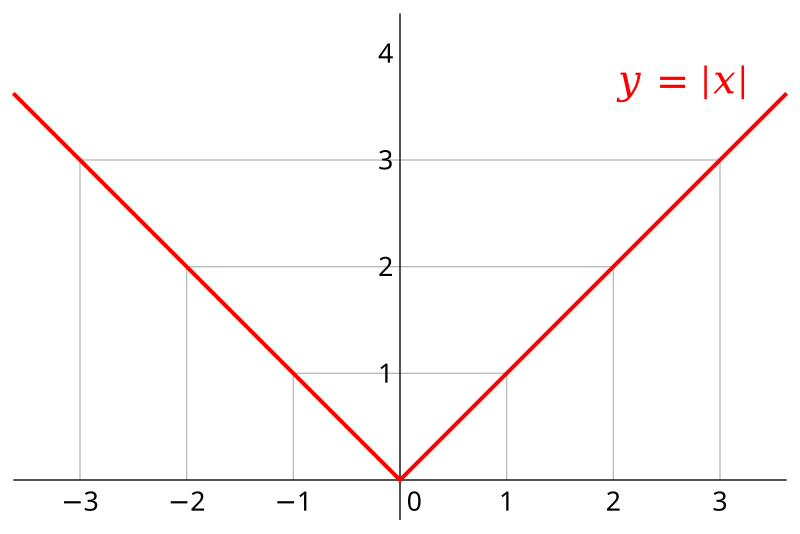
\includegraphics[width=0.5\linewidth, height=5cm, keepaspectratio]{images/basic_math/Absolute_value.svg.png}
            \caption{Absolute Value function/ Modulus Function \cite{wiki/Absolute-value}}
        \end{figure}
    \end{minipage}
\end{table}

\begin{lstlisting}[
    language=Python, 
    caption=Absolute value function
]
def get_absolute_value(val):
    if val >= 0:
        return val
    else:
        return -1 * val
\end{lstlisting}

\subsection*{Properties}

\subsubsection*{Fundamental properties \cite{wiki/Absolute-value}} \label{Basic Functions/Absolute Value function or Modulus Function/Fundamental properties}

\begin{customArrayStretch}{1.2}
\begin{tabular}{r l l}
     1. & ${\displaystyle |a|\geq 0}$ & Non-negativity \\
     
     2. & ${\displaystyle |a|=0\iff a=0}$ & Positive-definiteness \\
     
     3. & ${\displaystyle |ab|=\left|a\right|\left|b\right|}$ & 	Multiplicativity \\
     
     4. & ${\displaystyle |a+b|\leq |a|+|b|}$ & 	Subadditivity, specifically the triangle inequality \\
\end{tabular}
\end{customArrayStretch}

\subsubsection*{Additional useful properties \cite{wiki/Absolute-value}} \label{Basic Functions/Absolute Value function or Modulus Function/Additional useful properties}

\begin{customArrayStretch}{1.5}
\begin{tabular}{r l p{13cm}}
     1. & ${\displaystyle {\bigl |}\left|a\right|{\bigr |}=|a|}$ & 	Idempotence (the absolute value of the absolute value is the absolute value) \\
     
     2. & ${\displaystyle \left|-a\right|=|a|}$ & Evenness (reflection symmetry of the graph) \\
     
     3. & ${\displaystyle |a-b|=0\iff a=b}$ & 	Identity of indiscernibles (equivalent to positive-definiteness) \\
     
     4. & ${\displaystyle |a-b|\leq |a-c|+|c-b|}$ & 	Triangle inequality (equivalent to subadditivity) \\
     
     5. & ${\displaystyle \left|{\frac {a}{b}}\right|={\frac {|a|}{|b|}}\ }$ (if ${\displaystyle b\neq 0}$) & 	Preservation of division (equivalent to multiplicativity) \\
     
     6. & ${\displaystyle |a-b|\geq {\bigl |}\left|a\right|-\left|b\right|{\bigr |}}$ & 	Reverse triangle inequality (equivalent to subadditivity) \\
\end{tabular}
\end{customArrayStretch}

\subsection*{Inequalities} \label{Basic Functions/Absolute Value function or Modulus Function/Inequalities}

\begin{enumerate}
    \item ${\displaystyle |a|\leq b\iff -b\leq a\leq b}$

    \item ${\displaystyle |a|\geq b\iff b\leq a\leq -b\ }$

\end{enumerate}

\subsection*{Derivative} \label{Basic Functions/Absolute Value function or Modulus Function/Derivative}

\begin{enumerate}
    \item $
        {\displaystyle {\frac {d\left|x\right|}{dx}}={\frac {x}{|x|}}={\begin{cases}-1&x<0\\1&x>0\end{cases}}}
    $

    \item $
        {\displaystyle {d \over dx}f(|x|)={x \over |x|}(f'(|x|))}
    $ \hfill (discontinuous at $x=0$)

    \item $
        {\displaystyle {d \over dx}|f(x)|={f(x) \over |f(x)|}f'(x)}
    $ \hfill (discontinuous at $f(x)=0$)
\end{enumerate}


\subsection*{Anti-derivative/ Integral} \label{Basic Functions/Absolute Value function or Modulus Function/Anti-derivative or Integral}

$
    {\displaystyle \dint \left|x\right|dx={\dfrac {x\left|x\right|}{2}}+C}
$






\partition{Data}
\chapter{Data}

\section{Measurement Levels \cite{statistics/book/Statistics-for-Data-Scientists/Maurits-Kaptein}}\label{Data/Measurement-Levels}

\subsection{Nominal, Ordinal, Interval and Ratio \cite{statistics/book/Statistics-for-Data-Scientists/Maurits-Kaptein}}\label{Data/Measurement-Levels/Nominal, Ordinal, Interval and Ratio}

\label{Data/Measurement-Levels/Nominal, Ordinal, Interval and Ratio/Categorical Data}
\label{Data/Measurement-Levels/Nominal, Ordinal, Interval and Ratio/Numerical Data}
\label{Data/Measurement-Levels/Nominal, Ordinal, Interval and Ratio/Nominal}
\label{Data/Measurement-Levels/Nominal, Ordinal, Interval and Ratio/Ordinal}
\label{Data/Measurement-Levels/Nominal, Ordinal, Interval and Ratio/Interval}
\label{Data/Measurement-Levels/Nominal, Ordinal, Interval and Ratio/Ratio}

\begin{table}[H]
    \hfill
    \begin{minipage}[H]{0.25\linewidth}
        \textbf{Levels}: \cite{statistics/book/Statistics-for-Data-Scientists/Maurits-Kaptein}
        \begin{enumerate}
            \item Nominal
            \item Ordinal
            \item Interval
            \item Ratio
        \end{enumerate}
    \end{minipage}
    \hfill
    \begin{minipage}[H]{0.65\linewidth}
        \begin{table}[H]
            \centering
            \begin{tabular}{|p{5cm}|c|c|c|c|}
                \hline
                & \multicolumn{2}{c|}{\textbf{Categorical Data}} & \multicolumn{2}{c|}{\textbf{Numerical Data}} \\ 
                
                \hline
                & \textbf{Nominal} & \textbf{Ordinal} & \textbf{Interval} & \textbf{Ratio} \\ \hline
                
                Distinction between groups / individuals & \checkmark & \checkmark & \checkmark & \checkmark \\ \hline
                
                Imposes logical Order & \xmark & \checkmark & \checkmark & \checkmark \\ \hline
                
                Provides a magnitude of the differences in some unit & \xmark & \xmark & \checkmark & \checkmark \\ \hline
                
                A clear reference point or "0" & \xmark & \xmark & \xmark & \checkmark \\ \hline
            \end{tabular}
            \caption{Data: Measurement Levels: Nominal, Ordinal, Interval and Ratio \cite{statistics/book/Statistics-for-Data-Scientists/Maurits-Kaptein}}
        \end{table}
    \end{minipage}
    \hfill
\end{table}

\vspace{0.3cm}

\textbf{Note}:
\begin{enumerate}
    \item Each consecutive measurement level contains as much "information" - in a fairly loose sense of the word - as the previous one and more. \cite{statistics/book/Statistics-for-Data-Scientists/Maurits-Kaptein}
\end{enumerate}


\subsection{Continuous vs Discrete numerical data \cite{statistics/book/Statistics-for-Data-Scientists/Maurits-Kaptein}}\label{Data/Measurement-Levels/Continuous vs Discrete numerical data}

\label{Data/Measurement-Levels/Continuous vs Discrete numerical data/Continuous numerical data}
\label{Data/Measurement-Levels/Continuous vs Discrete numerical data/Discrete numerical data}

\begin{enumerate}
    \item Continuous variables can assume any value.\\
    This means that the continuous variable can attain any value between two different values, no matter how close the two values are.\\
    \textbf{Example}: temperature, weight, and age

    \item Discrete variables cannot assume any value between 2 values\\
    \textbf{Example}: number of text messages, accidents, microorganisms, students, etc.
\end{enumerate}


\subsection{Outliers \cite{statistics/book/Statistics-for-Data-Scientists/Maurits-Kaptein}}\label{Data/Measurement-Levels/Outliers}

\begin{enumerate}
    \item An outlier is a data point that significantly deviates from other observations in a dataset. \cite{common/online/chatgpt}

    \item Caused by Natural variability in the data or measurement errors. \cite{common/online/chatgpt}

    \item Typically identified using statistical methods like the IQR (Interquartile Range), Z-score, or visualization techniques (e.g., box plots). \cite{common/online/chatgpt}

    \item Outliers are not necessarily incorrect; they may represent rare but valid observations. \cite{common/online/chatgpt}
    
\end{enumerate}


\vspace{0.3cm}

\textbf{Examples}:
\begin{enumerate}
    \item In a dataset of human heights, a person measuring 250 cm might be an outlier but not necessarily unrealistic if it’s a rare case of gigantism. \cite{common/online/chatgpt}
\end{enumerate}


\vspace{0.3cm}
\textbf{Handling/ Dealing with Outliers}:
\begin{enumerate}
    \item Ignore these abnormalities and go ahead with the data. \cite{statistics/book/Statistics-for-Data-Scientists/Maurits-Kaptein}

    \item Delete/ remove the suspected records/ entries. \cite{statistics/book/Statistics-for-Data-Scientists/Maurits-Kaptein}

    \item Substitute them, using statistical methods, with a more plausible alternative. (aka \textbf{imputation}) \cite{statistics/book/Statistics-for-Data-Scientists/Maurits-Kaptein}\label{Data/Outliers/imputation}
\end{enumerate}




\subsection{Unrealistic Values \cite{statistics/book/Statistics-for-Data-Scientists/Maurits-Kaptein}}\label{Data/Measurement-Levels/Unrealistic Values}

\begin{enumerate}
    \item An unrealistic value is a data point that is not plausible within the context of the dataset, often due to data entry errors or faulty sensors. \cite{common/online/chatgpt}

    \item Caused by Human error, sensor malfunction, or corruption during data transmission. \cite{common/online/chatgpt}

    \item Typically identified using domain knowledge or logical constraints. \cite{common/online/chatgpt}

    \item Unlike outliers, unrealistic values are generally not useful and need correction or removal. \cite{common/online/chatgpt}

\end{enumerate}

\vspace{0.3cm}

\textbf{Examples}:
\begin{enumerate}
    \item A recorded body temperature of 200°C for a human is unrealistic, as it’s physically impossible for a person to survive at that temperature. \cite{common/online/chatgpt}

    \item Negative age of a person \cite{common/online/chatgpt}

    \item Missing values \cite{statistics/book/Statistics-for-Data-Scientists/Maurits-Kaptein}

    \item Incorrect datatype of value \cite{statistics/book/Statistics-for-Data-Scientists/Maurits-Kaptein}
\end{enumerate}

\vspace{0.3cm}
\textbf{Handling/ Dealing with Unrealistic values}:
\begin{enumerate}
    \item Delete/ remove the suspected records/ entries. \cite{statistics/book/Statistics-for-Data-Scientists/Maurits-Kaptein}
    
\end{enumerate}





\section{Describing Data \cite{statistics/book/Statistics-for-Data-Scientists/Maurits-Kaptein}} \label{Data/Describing Data}

Some \textbf{descriptive statistics}\label{Data/Describing Data/descriptive statistics} (or just \textbf{descriptives}\label{Data/Describing Data/descriptives}) that we introduce are often used for data of a certain measurement level. \cite{statistics/book/Statistics-for-Data-Scientists/Maurits-Kaptein}

\subsection{Frequency/ Frequency table \cite{statistics/book/Statistics-for-Data-Scientists/Maurits-Kaptein}}\label{Data/Describing Data/Frequency or Frequency table}

\textbf{Measurement levels}: Nominal and ordinal data

\vspace{0.3cm}

\begin{enumerate}
    \item Frequencies are often uninformative for interval or ratio variables. \cite{statistics/book/Statistics-for-Data-Scientists/Maurits-Kaptein}\\
        if there are lots and lots of different possible values, all of them will have a count of just one. \cite{statistics/book/Statistics-for-Data-Scientists/Maurits-Kaptein}\\
        This is often tackled by discretizing (or "\textbf{binning}”\label{Data/Describing Data/Frequency or Frequency table/binning}) the variable (which, note, effectively "throws away” some of the information in the data). \cite{statistics/book/Statistics-for-Data-Scientists/Maurits-Kaptein}

    
\end{enumerate}


\subsubsection{(Absolute) Frequency/ (Absolute) Frequency table \cite{statistics/book/Statistics-for-Data-Scientists/Maurits-Kaptein}}\label{Data/Describing Data/Frequency or Frequency table/Absolute}

\begin{enumerate}
    \item It refers to the count of occurrences of a particular value or category in a dataset. \cite{common/online/chatgpt}

    \item Simple count, no further processing. \cite{common/online/chatgpt}

    \item \textbf{Use Case}: Helpful in creating bar charts or histograms. \cite{common/online/chatgpt}
\end{enumerate}



\subsubsection{Cumulative Frequency/ Cumulative Frequency table \cite{statistics/book/Statistics-for-Data-Scientists/Maurits-Kaptein}}\label{Data/Describing Data/Frequency or Frequency table/Cumulative}

\begin{enumerate}
    \item It is the running total of frequencies up to a certain value or class. \cite{common/online/chatgpt}

    \item Each cumulative frequency includes its own frequency plus all previous frequencies. \cite{common/online/chatgpt}

    \item \textbf{Use Case}: Useful in percentile calculations and ogive graphs. \cite{common/online/chatgpt}

    \item The cumulative frequency makes more sense for ordinal data than for nominal data, since ordinal data can be ordered in size, which is not possible for nominal data. \cite{statistics/book/Statistics-for-Data-Scientists/Maurits-Kaptein}
\end{enumerate}

\begin{table}[H]
    \begin{minipage}[H]{0.3\linewidth}
    $
        \begin{aligned}
            CF_i 
                &= CF_{i-1} + F_{i} \\
                &= \sum_{k=1}^{i} F_{k}
        \end{aligned}
    $
    \end{minipage}
    \begin{minipage}[H]{0.65\linewidth}
        \begin{table}[H]
            \begin{tabular}{l l}
                $CF_i$ & Cumulative Frequency at the current value \\ 
                $CF_{i-1}$ & Cumulative Frequency at the previous value \\ 
                $F_i$ & Frequency at the current value \\ 
            \end{tabular}
            \caption*{Notations}
        \end{table}
    \end{minipage}
\end{table}


\subsubsection{Relative Frequency/ Relative Frequency table \cite{statistics/book/Statistics-for-Data-Scientists/Maurits-Kaptein}}\label{Data/Describing Data/Frequency or Frequency table/Relative}

\begin{enumerate}
    \item It shows the proportion of each category relative to the total number of observations. \cite{common/online/chatgpt}

    \item Expressed as a fraction, decimal, or percentage. \cite{common/online/chatgpt}

    \item \textbf{Use Case}: Ideal for creating pie charts and understanding distribution proportions. \cite{common/online/chatgpt}
\end{enumerate}


\begin{table}[H]
    \begin{minipage}{0.3\linewidth}
        \[
            \begin{aligned}
                RF_i 
                    &= \dfrac{F_{i}}{\dsum_{k=1}^{N} F_{k}}
            \end{aligned}
        \]
    \end{minipage}
    \begin{minipage}{0.65\linewidth}
        \begin{table}[H]
            \begin{tabular}{l l}
                $RF_i$ & Relative Frequency \\
                $F_i$ & Frequency of the value \\ 
                $N$ & Total number of observations \\ 
            \end{tabular}
            \caption*{Notations}
        \end{table}
    \end{minipage}
\end{table}




\subsubsection{Cumulative Relative Frequency/ Cumulative Relative Frequency table \cite{statistics/book/Statistics-for-Data-Scientists/Maurits-Kaptein}}\label{Data/Describing Data/Frequency or Frequency table/Cumulative Relative}

\begin{enumerate}
    \item Cumulative relative frequency is the accumulation of the relative frequencies of data points up to a certain value. \cite{common/online/chatgpt}

    \item It indicates the proportion of data points that are less than or equal to a particular value. \cite{common/online/chatgpt}

    \item \textbf{Use Cases}:
    \begin{enumerate}
        \item Identifying percentiles and median.

        \item Visualizing with a cumulative relative frequency graph (Ogive).

        \item Understanding data distribution by determining the proportion of values below a specific threshold.
    \end{enumerate}
\end{enumerate}



\begin{table}[H]
    \begin{minipage}{0.3\linewidth}
        \[
            \begin{aligned}
                CRF_i 
                    &= \dfrac{\dsum_{k=1}^{i} F_{k}}{\dsum_{k=1}^{N} F_{k}}
            \end{aligned}
        \]
    \end{minipage}
    \begin{minipage}{0.65\linewidth}
        \begin{table}[H]
            \begin{tabular}{l l}
                $CRF_i$ & Cumulative Relative Frequency \\
                $F_i$ & Frequency of the value \\ 
                $N$ & Total number of observations \\ 
            \end{tabular}
            \caption*{Notations}
        \end{table}
    \end{minipage}
\end{table}





\subsection{Central Tendency \cite{statistics/book/Statistics-for-Data-Scientists/Maurits-Kaptein}}\label{Data/Describing Data/Central Tendency}

\begin{enumerate}
     \item When we work with numerical data, we often want to know something about the "central value" or "middle value" of the variable, also referred to as the \textbf{location}\label{Data/Describing Data/Central Tendency/location} of the data. \cite{statistics/book/Statistics-for-Data-Scientists/Maurits-Kaptein}
\end{enumerate}


\subsubsection{(Arithmetic) mean/ average \cite{statistics/book/Statistics-for-Data-Scientists/Maurits-Kaptein}} \label{Data/Describing Data/Central Tendency/(Arithmetic) mean or average}

\begin{table}[H]
    \begin{minipage}{0.3\linewidth}
        $
            \bar{x} = \dfrac{1}{n} \dsum_{i=1}^{n} x_i
        $
    \end{minipage}
    \begin{minipage}{0.65\linewidth}
        \begin{table}[H]
            \begin{tabular}{l l}
                $\bar{x}$ & mean \\
                $x_i$ & item \\
                $n$ & number of items \\
            \end{tabular}
            \caption*{Notations}
        \end{table}
    \end{minipage}
\end{table}



\subsubsection{Mode \cite{statistics/book/Statistics-for-Data-Scientists/Maurits-Kaptein}} \label{Data/Describing Data/Central Tendency/Mode}

\begin{enumerate}
    \item The mode is merely the most frequently occurring value. \cite{statistics/book/Statistics-for-Data-Scientists/Maurits-Kaptein}

    \item There might be multiple modes. \cite{statistics/book/Statistics-for-Data-Scientists/Maurits-Kaptein}
    
\end{enumerate}



\subsubsection{Median \cite{statistics/book/Statistics-for-Data-Scientists/Maurits-Kaptein}} \label{Data/Describing Data/Central Tendency/Median}

\begin{enumerate}
    \item The median is a value that divides the ordered data from small to large (or large to small) into two equal parts: 50\% of the data is below the median and 50\% is above. \cite{statistics/book/Statistics-for-Data-Scientists/Maurits-Kaptein}

    \item The median is not necessarily a value that is present in the data. \cite{statistics/book/Statistics-for-Data-Scientists/Maurits-Kaptein}
\end{enumerate}


\vspace{0.3cm}
\textbf{Steps}:
\begin{enumerate}
    \item sort the data

    \item choose the middle-most value when $n$ is \textbf{odd}\\
        average of the two middle values when $n$ is \textbf{even}
\end{enumerate}



\subsubsection{Quantiles \cite{statistics/book/Statistics-for-Data-Scientists/Maurits-Kaptein}} \label{Data/Describing Data/Central Tendency/Quantiles}

\begin{enumerate}
    \item A quantile $x_q$ is a value that splits the ordered data of a variable $x$ into two parts: \cite{statistics/book/Statistics-for-Data-Scientists/Maurits-Kaptein}
    \begin{enumerate}
        \item $q \cdot 100\%$ of the data is below the value $x_q$

        \item $(1 - q) \cdot 100\%$ of the data is above the value $x_q$
    \end{enumerate}
    
    \item The parameter $q$ can take any value in the interval $[0, 1]$. \cite{statistics/book/Statistics-for-Data-Scientists/Maurits-Kaptein}

    \item Quantiles can be calculated in different ways, depending on the way we "interpolate" between two values. \cite{statistics/book/Statistics-for-Data-Scientists/Maurits-Kaptein} \\
    We could map the ordered values \textit{equally spaced} on the interval $(0, 1)$, where the \textit{i}th ordered value of the data is positioned at the level $q_i = {i}/{(n + 1)}$ in the interval $(0, 1)$, with $n$ being the number of data points. \cite{statistics/book/Statistics-for-Data-Scientists/Maurits-Kaptein} \\
    R uses $q_i = (i - 1)/(n - 1)$ for quantiles. \cite{statistics/book/Statistics-for-Data-Scientists/Maurits-Kaptein} \\
    \textbf{Example}: \cite{statistics/book/Statistics-for-Data-Scientists/Maurits-Kaptein}
    \begin{enumerate}
        \item Data points: $\dCurlyBrac{2, 5, 6, 4}$ ($n=4$)
        \item Sorted Data points: $\dCurlyBrac{2, 4, 5, 6}$ ($n=4$)
        \item Quantiles:\\[0.2cm]
        \begin{tabular}{|l|c|c|c|}
            \hline
            $i$ & $x_i$ & $q_i = i/(n+1) = i/5$ & $q_i = (i-1)/(n-1) = (i-1)/3$ \\ [0.1cm]
            \hline
            $1$ & $2$ & $1/5 = 0.2$ & $0$ \\
            $2$ & $4$ & $2/5 = 0.4$ & $1/3$ \\
            $3$ & $5$ & $3/5 = 0.6$ & $2/3$ \\
            $4$ & $6$ & $4/5 = 0.8$ & $1$ \\
            \hline
        \end{tabular}\\

        \item If $x_i = 3 \Rightarrow q_i = 0.3$
    \end{enumerate}
\end{enumerate}




\subsubsection{Quartiles \cite{statistics/book/Statistics-for-Data-Scientists/Maurits-Kaptein}} \label{Data/Describing Data/Central Tendency/Quartiles}

\begin{enumerate}
    \item When $q = 0.25$, $q = 0.50$, and $q = 0.75$ the quantiles are referred to as the first, second, and third quartiles, respectively. \cite{statistics/book/Statistics-for-Data-Scientists/Maurits-Kaptein}
    \label{Data/Describing Data/Central Tendency/Quartiles/first quartile}
    \label{Data/Describing Data/Central Tendency/Quartiles/second quartile}
    \label{Data/Describing Data/Central Tendency/Quartiles/third quartile}

    \item Splits: \\
    \begin{tabular}{r l l l} % Right-align first column, left-align second column
        1. & $q = 0$ & to & $q = 0.25$ \\
        2. & $q = 0.25$ & to & $q = 0.5$ \\
        3. & $q = 0.5$ & to & $q = 0.75$ \\
        4. & $q = 0.75$ & to & $q = 1$ \\
    \end{tabular}
\end{enumerate}



\subsubsection{Deciles \cite{statistics/book/Statistics-for-Data-Scientists/Maurits-Kaptein}} \label{Data/Describing Data/Central Tendency/Deciles}

\begin{enumerate}
    \item We call quantiles deciles when $q$ is restricted to the set $\dCurlyBrac{0.1, 0.2,\cdots, 0.9}$

    \item Splits: \\
    \begin{tabular}{r l l l} % Right-align first column, left-align second column
        1. & $q = 0$ & to & $q = 0.1$ \\
        2. & $q = 0.1$ & to & $q = 0.2$ \\
        && \vdots & \\
        9. & $q = 0.8$ & to & $q = 0.9$ \\
        10. & $q = 0.9$ & to & $q = 1$ \\
    \end{tabular}
\end{enumerate}



\subsubsection{Percentiles \cite{statistics/book/Statistics-for-Data-Scientists/Maurits-Kaptein}} \label{Data/Describing Data/Central Tendency/Percentiles}

\begin{enumerate}
    \item We call quantiles percentiles when $q$ is restricted to the set $\dCurlyBrac{0.01, 0.02,\cdots, 0.99}$

    \item Splits: \\
    \begin{tabular}{r l l l} % Right-align first column, left-align second column
        1. & $q = 0$ & to & $q = 0.01$ \\
        2. & $q = 0.01$ & to & $q = 0.02$ \\
        & & \vdots & \\
        99. & $q = 0.98$ & to & $q = 0.99$ \\
        100. & $q = 0.99$ & to & $q = 1$ \\
    \end{tabular}
\end{enumerate}









\chapter{Visualizing Data} \label{Visualizing Data}

\begin{enumerate}
    \item Visualization, when done well, can make large and even high-dimensional datasets (relatively) easy to interpret. \hfill \cite{statistics/book/Statistics-for-Data-Scientists/Maurits-Kaptein}

    
\end{enumerate}


\begin{lstlisting}[
    language=Python
]
import random
import faker                    # to generate fake data
import numpy as np
import pandas as pd
from tqdm import tqdm           # progress bar

# plotting libraries
import seaborn as sns           
import matplotlib.pyplot as plt

random.seed(0)
np.random.seed(0)
faker.Faker.seed(0)

fake = faker.Faker()
\end{lstlisting}


\clearpage
\section{Box and Whiskers Plot/ Box Plot \cite{data/online/seaborn.boxplot, data/online/matplotlib.pyplot.boxplot}} \label{Visualizing Data/Box and Whiskers Plot or Box Plot}

\begin{lstlisting}[numbers=none]

                     Q1-1.5IQR   Q1   median  Q3   Q3+1.5IQR
                                  |-----:-----|
                  o      |--------|     :     |--------|    o  o
                                  |-----:-----|
                flier             <----------->            fliers
                                       IQR

\end{lstlisting}

\vspace{0.5cm}

\begin{table}[H]
\begin{minipage}[t]{0.35\linewidth}
\begin{figure}[H]
    \centering
    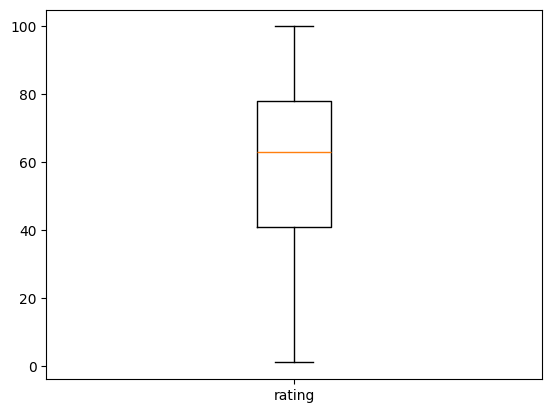
\includegraphics[width=0.9\linewidth, height=10cm, keepaspectratio]{images/data/__visualizations__/plt-box-rating-face-data.png}
    \caption{Box and Whiskers plot (py-plt) output (face\_data.csv)}
\end{figure}
\end{minipage}
\hspace{0.2cm}
\vrule width 1pt
\hspace{0.5cm}
\begin{minipage}[t]{0.57\linewidth}
\begin{lstlisting}[
    language=Python,
    caption=Box and Whiskers Plot: py-plt: face\_data.csv
]
_col = "rating"

plt.boxplot(df[_col])
plt.xticks([1], [_col])
plt.show()
\end{lstlisting}
\end{minipage}
\end{table}



\begin{table}[H]
\begin{minipage}[t]{0.35\linewidth}
\begin{figure}[H]
    \centering
    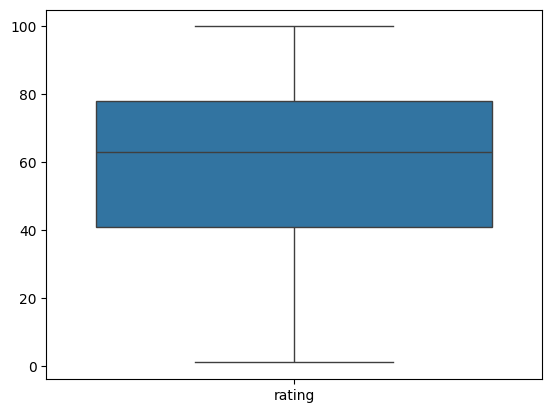
\includegraphics[width=0.9\linewidth, height=10cm, keepaspectratio]{images/data/__visualizations__/sns-box-rating-face-data.png}
    \caption{Box and Whiskers plot (py-sns) output (face\_data.csv)}
\end{figure}
\end{minipage}
\hspace{0.2cm}
\vrule width 1pt
\hspace{0.5cm}
\begin{minipage}[t]{0.57\linewidth}
\begin{lstlisting}[
    language=Python,
    caption=Box and Whiskers Plot: py-sns: face\_data.csv
]
_col = "rating"

sns.boxplot(df[_col])
plt.ylabel("")
plt.xticks([0], [_col])
plt.show()
\end{lstlisting}
\end{minipage}
\end{table}




\begin{enumerate}
    \item A box plot (or box-and-whisker plot) shows the distribution of quantitative data in a way that facilitates comparisons between variables or across levels of a categorical variable.  \hfill \cite{data/online/seaborn.boxplot}
    
    \item The box shows the quartiles of the dataset while the whiskers extend to show the rest of the distribution, except for points that are determined to be “outliers” using a method that is a function of the inter-quartile range. \hfill \cite{data/online/seaborn.boxplot}
\end{enumerate}





\clearpage
\section{Count Plot \cite{data/online/seaborn.countplot}} \label{Visualizing Data/Count Plot}


\begin{table}[H]
\begin{minipage}[t]{0.35\linewidth}
\begin{figure}[H]
    \centering
    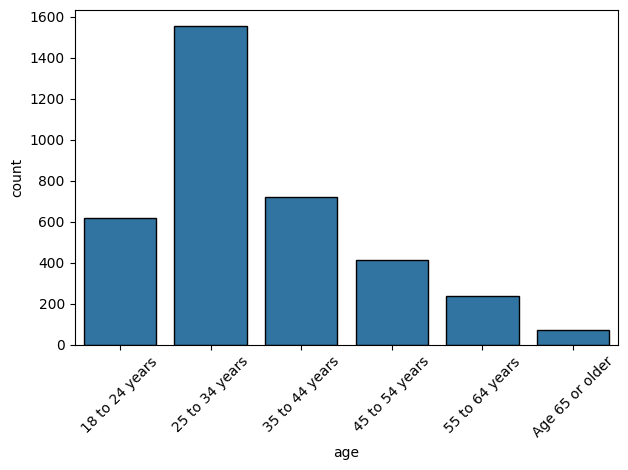
\includegraphics[width=0.9\linewidth, height=10cm, keepaspectratio]{images/data/__visualizations__/sns-countplot-face-data.png}
    \caption{Count plot (py-sns) output (face\_data.csv)}
\end{figure}
\end{minipage}
\hspace{0.2cm}
\vrule width 1pt
\hspace{0.5cm}
\begin{minipage}[t]{0.57\linewidth}
\begin{lstlisting}[
    language=Python,
    caption=Count Plot: py-sns: face\_data.csv
]
vals = df[df["age"] != " "].copy()

sns.countplot(
    x='age', 
    data=vals, 
    order=sorted(vals['age'].unique()), 
    edgecolor='black',
)

plt.xticks(rotation=45)
plt.tight_layout()
plt.show()
\end{lstlisting}
\end{minipage}
\end{table}

\vspace{0.3cm}

\begin{enumerate}
    \item Show the counts of observations in each categorical bin using bars.

    
\end{enumerate}



% \clearpage
\section{Density Plot \cite{data/online/seaborn.displot}} \label{Visualizing Data/Density Plot}

\begin{table}[H]
\begin{minipage}[t]{0.35\linewidth}
\begin{figure}[H]
    \centering
    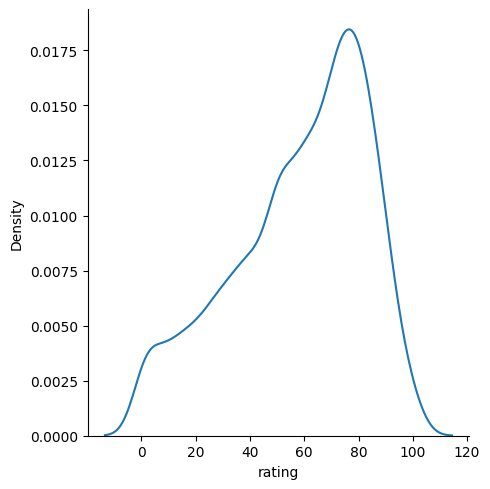
\includegraphics[width=0.9\linewidth, height=10cm, keepaspectratio]{images/data/__visualizations__/sns-density-kde-rating-face-data.png}
    \caption{Density plot (py-sns) output (face\_data.csv)}
\end{figure}
\end{minipage}
\hspace{0.2cm}
\vrule width 1pt
\hspace{0.5cm}
\begin{minipage}[t]{0.57\linewidth}
\begin{lstlisting}[
    language=Python,
    caption=Density Plot: py-sns: face\_data.csv
]
sns.displot(df["rating"], kind="kde")

plt.show()
\end{lstlisting}

\vspace{0.2cm}

\begin{enumerate}
    \item A density plot - at least in this setting - can be considered a “continuous approximation” of a histogram. \hfill \cite{statistics/book/Statistics-for-Data-Scientists/Maurits-Kaptein} \\
    SEE: \fullref{Visualizing Data/Histogram}

    \item It gives per range of values of the continuous variable the probability of observing a value within that range. \hfill \cite{statistics/book/Statistics-for-Data-Scientists/Maurits-Kaptein}


\end{enumerate}

\end{minipage}
\end{table}







\clearpage
\section{Histogram \cite{data/online/seaborn.histplot}} \label{Visualizing Data/Histogram}


\begin{table}[H]
\begin{minipage}[t]{0.35\linewidth}
\begin{figure}[H]
    \centering
    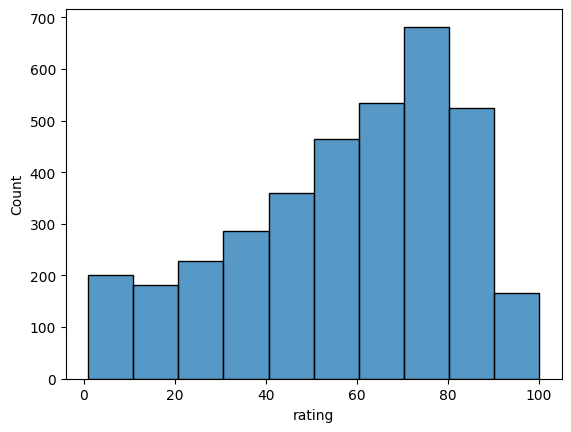
\includegraphics[width=0.9\linewidth, height=10cm, keepaspectratio]{images/data/__visualizations__/sns-hist-rating-face-data.png}
    \caption{Histogram (py-sns) output (face\_data.csv)}
\end{figure}
\end{minipage}
\hspace{0.2cm}
\vrule width 1pt
\hspace{0.5cm}
\begin{minipage}[t]{0.57\linewidth}
\begin{lstlisting}[
    language=Python,
    caption=Histogram: py-sns: face\_data.csv
]
sns.histplot(df["rating"], binwidth=10)
plt.show()
\end{lstlisting}

\vspace{0.2cm}

\begin{enumerate}
    \item A histogram is a classic visualization tool that represents the distribution of one or more variables by counting the number of observations that fall within discrete bins. \hfill \cite{data/online/seaborn.histplot}

    \item A histogram “bins” the data (discretizes it), and subsequently shows the frequency of occurrence in each bin. \hfill \cite{statistics/book/Statistics-for-Data-Scientists/Maurits-Kaptein}
    
    \item It is the continuous variant of the bar chart. \hfill \cite{statistics/book/Statistics-for-Data-Scientists/Maurits-Kaptein}\\
    SEE: \fullref{Visualizing Data/Box and Whiskers Plot or Box Plot}
    
    \item The number of bins selected makes a big difference in the visualization: too few bins obscure the patterns in the data, but too many bins lead to counts of exactly one for each value. \hfill \cite{statistics/book/Statistics-for-Data-Scientists/Maurits-Kaptein}
\end{enumerate}

\end{minipage}
\end{table}


% \clearpage
\section{Pairwise Plot \cite{statistics/book/Statistics-for-Data-Scientists/Maurits-Kaptein, data/online/seaborn.pairplot}} \label{Visualizing Data/Pairwise Plot}


\begin{table}[H]
\begin{minipage}[t]{0.35\linewidth}
\begin{figure}[H]
    \centering
    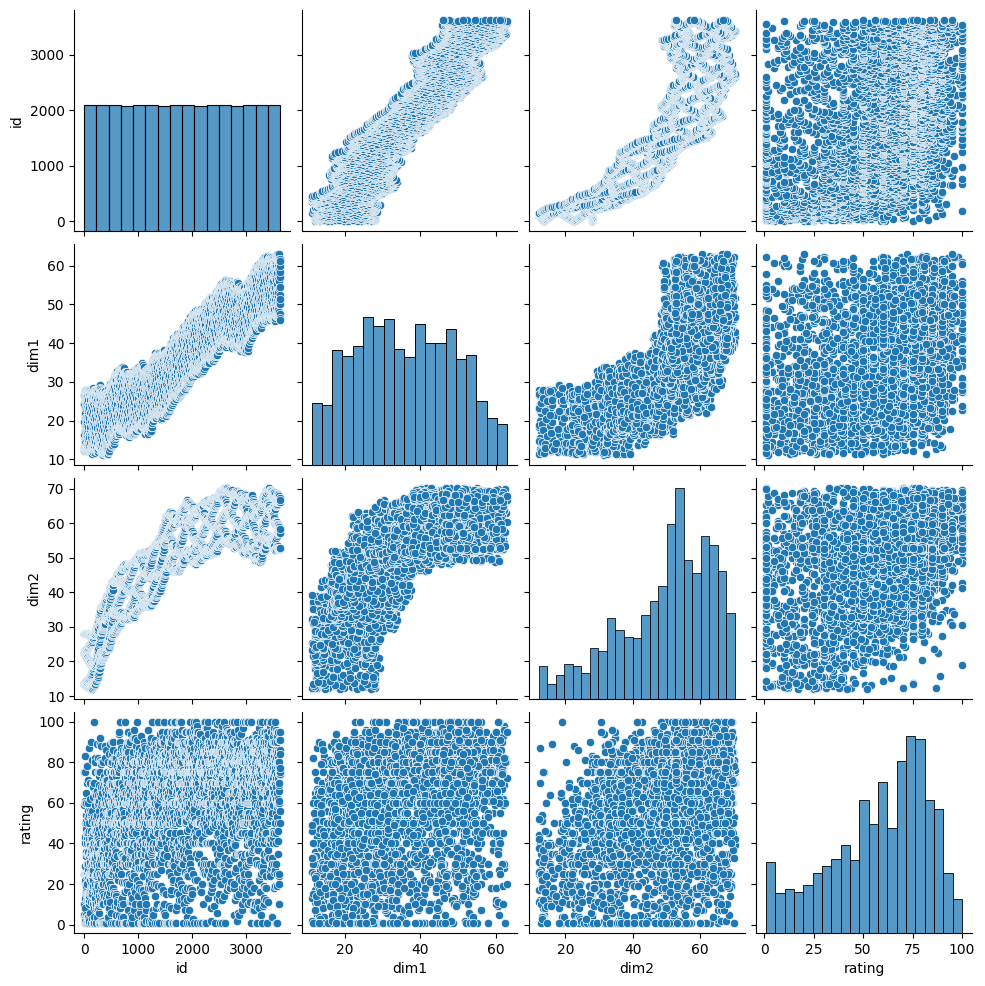
\includegraphics[width=0.9\linewidth, height=10cm, keepaspectratio]{images/data/__visualizations__/sns-pairplot-face-data.png}
    \caption{Pairwise plot (py-sns) output (face\_data.csv)}
\end{figure}
\end{minipage}
\hspace{0.2cm}
\vrule width 1pt
\hspace{0.5cm}
\begin{minipage}[t]{0.57\linewidth}
\begin{lstlisting}[
    language=Python,
    caption=Pairwise Plot: py-sns: face\_data.csv
]
df = pd.read_csv("face_data.csv")
sns.pairplot(df)
\end{lstlisting}

\vspace{0.3cm}

\begin{enumerate}
    \item Plot pairwise relationships in a dataset. \hfill \cite{data/online/seaborn.pairplot}

    \item By default, this is a grid of Axes such that each numeric variable in data will by shared across the y-axes across a single row and the x-axes across a single column. \hfill \cite{data/online/seaborn.pairplot}
    
    \item The diagonal plots are treated differently: a univariate distribution plot is drawn to show the marginal distribution of the data in each column. \hfill \cite{data/online/seaborn.pairplot}
\end{enumerate}
\end{minipage}
\end{table}











\clearpage
\section{Pie Chart \cite{data/online/matplotlib.pyplot.pie}} \label{Visualizing Data/Pie Chart}


\begin{table}[H]
\begin{minipage}[t]{0.35\linewidth}
\begin{figure}[H]
    \centering
    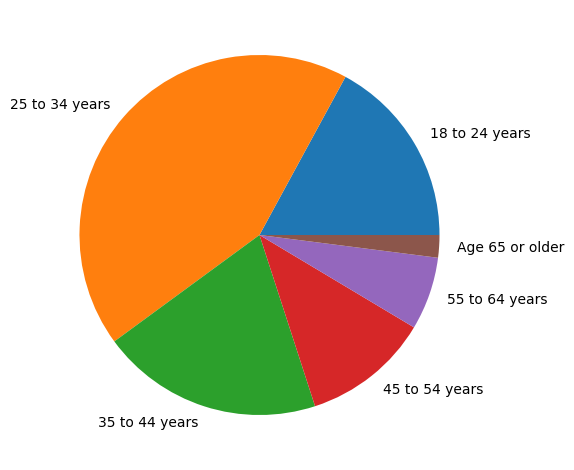
\includegraphics[width=0.9\linewidth, height=10cm, keepaspectratio]{images/data/__visualizations__/plt-pie-age-face-data.png}
    \caption{Pie chart (py-plt) output (face\_data.csv)}
\end{figure}
\end{minipage}
\hspace{0.2cm}
\vrule width 1pt
\hspace{0.5cm}
\begin{minipage}[t]{0.57\linewidth}
\begin{lstlisting}[
    language=Python,
    caption=Pie Chart: py-plt: face\_data.csv
]
vals = df[df["age"] != " "].copy()

labels, counts = np.unique(
    vals['age'],
    return_counts=True
)

plt.pie(counts, labels=labels)

plt.tight_layout()
plt.show()
\end{lstlisting}
\end{minipage}
\end{table}



\clearpage
\section{Scatter Plot \cite{data/online/seaborn.scatterplot, data/online/seaborn.scatterplot, data/online/wiki/Scatter_plot}} \label{Visualizing Data/Scatter Plot}


\begin{table}[H]
\begin{minipage}[t]{0.35\linewidth}
\begin{figure}[H]
    \centering
    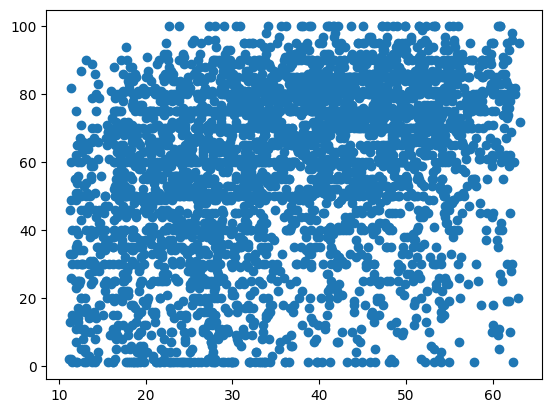
\includegraphics[width=0.9\linewidth, height=10cm, keepaspectratio]{images/data/__visualizations__/plt-scatter-dim1-rating-face-data.png}
    \caption{Scatter Plot (py-plt) output (face\_data.csv)}
\end{figure}
\end{minipage}
\hspace{0.2cm}
\vrule width 1pt
\hspace{0.5cm}
\begin{minipage}[t]{0.57\linewidth}
\begin{lstlisting}[
    language=Python,
    caption=Scatter Plot: py-plt: face\_data.csv
]
plt.scatter(df["dim1"], df["rating"])

plt.show()
\end{lstlisting}
\end{minipage}
\end{table}

\begin{table}[H]
\begin{minipage}[t]{0.35\linewidth}
\begin{figure}[H]
    \centering
    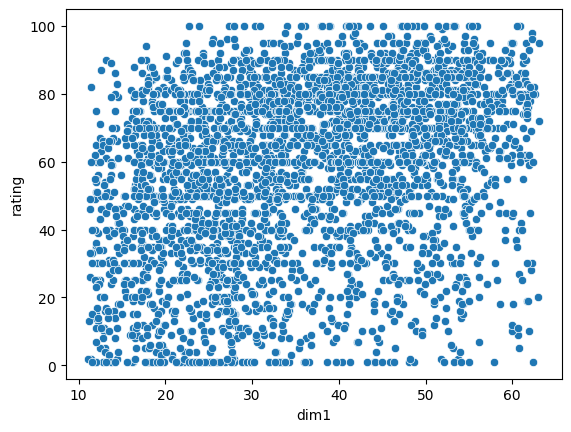
\includegraphics[width=0.9\linewidth, height=10cm, keepaspectratio]{images/data/__visualizations__/sns-scatter-dim1-rating-face-data.png}
    \caption{Scatter Plot (py-sns) output (face\_data.csv)}
\end{figure}
\end{minipage}
\hspace{0.2cm}
\vrule width 1pt
\hspace{0.5cm}
\begin{minipage}[t]{0.57\linewidth}
\begin{lstlisting}[
    language=Python,
    caption=Scatter Plot: py-sns: face\_data.csv
]
sns.scatterplot(df, x="dim1", y="rating")

plt.show()
\end{lstlisting}
\end{minipage}
\end{table}





\begin{enumerate}
    \item A scatter plot, also called a \textbf{scatterplot}, \textbf{scatter graph}\label{Visualizing Data/scatter graph}, \textbf{scatter chart}\label{Visualizing Data/scatter chart}, \textbf{scattergram}\label{Visualizing Data/scattergram}, or \textbf{scatter diagram}\label{Visualizing Data/scatter diagram}, is a type of plot or mathematical diagram using Cartesian coordinates to display values for typically two variables for a set of data. \hfill \cite{data/online/wiki/Scatter_plot}
    
    \item If the points are coded (color/shape/size), one additional variable can be displayed. \hfill \cite{data/online/wiki/Scatter_plot}
    
    \item The data are displayed as a collection of points, each having the value of one variable determining the position on the horizontal axis and the value of the other variable determining the position on the vertical axis. \hfill \cite{data/online/wiki/Scatter_plot}
\end{enumerate}











\partition{Mathematics: Statistics}
\chapter{Sampling Plans}\label{Sampling Plans}


\begin{figure}[H]
    \centering
    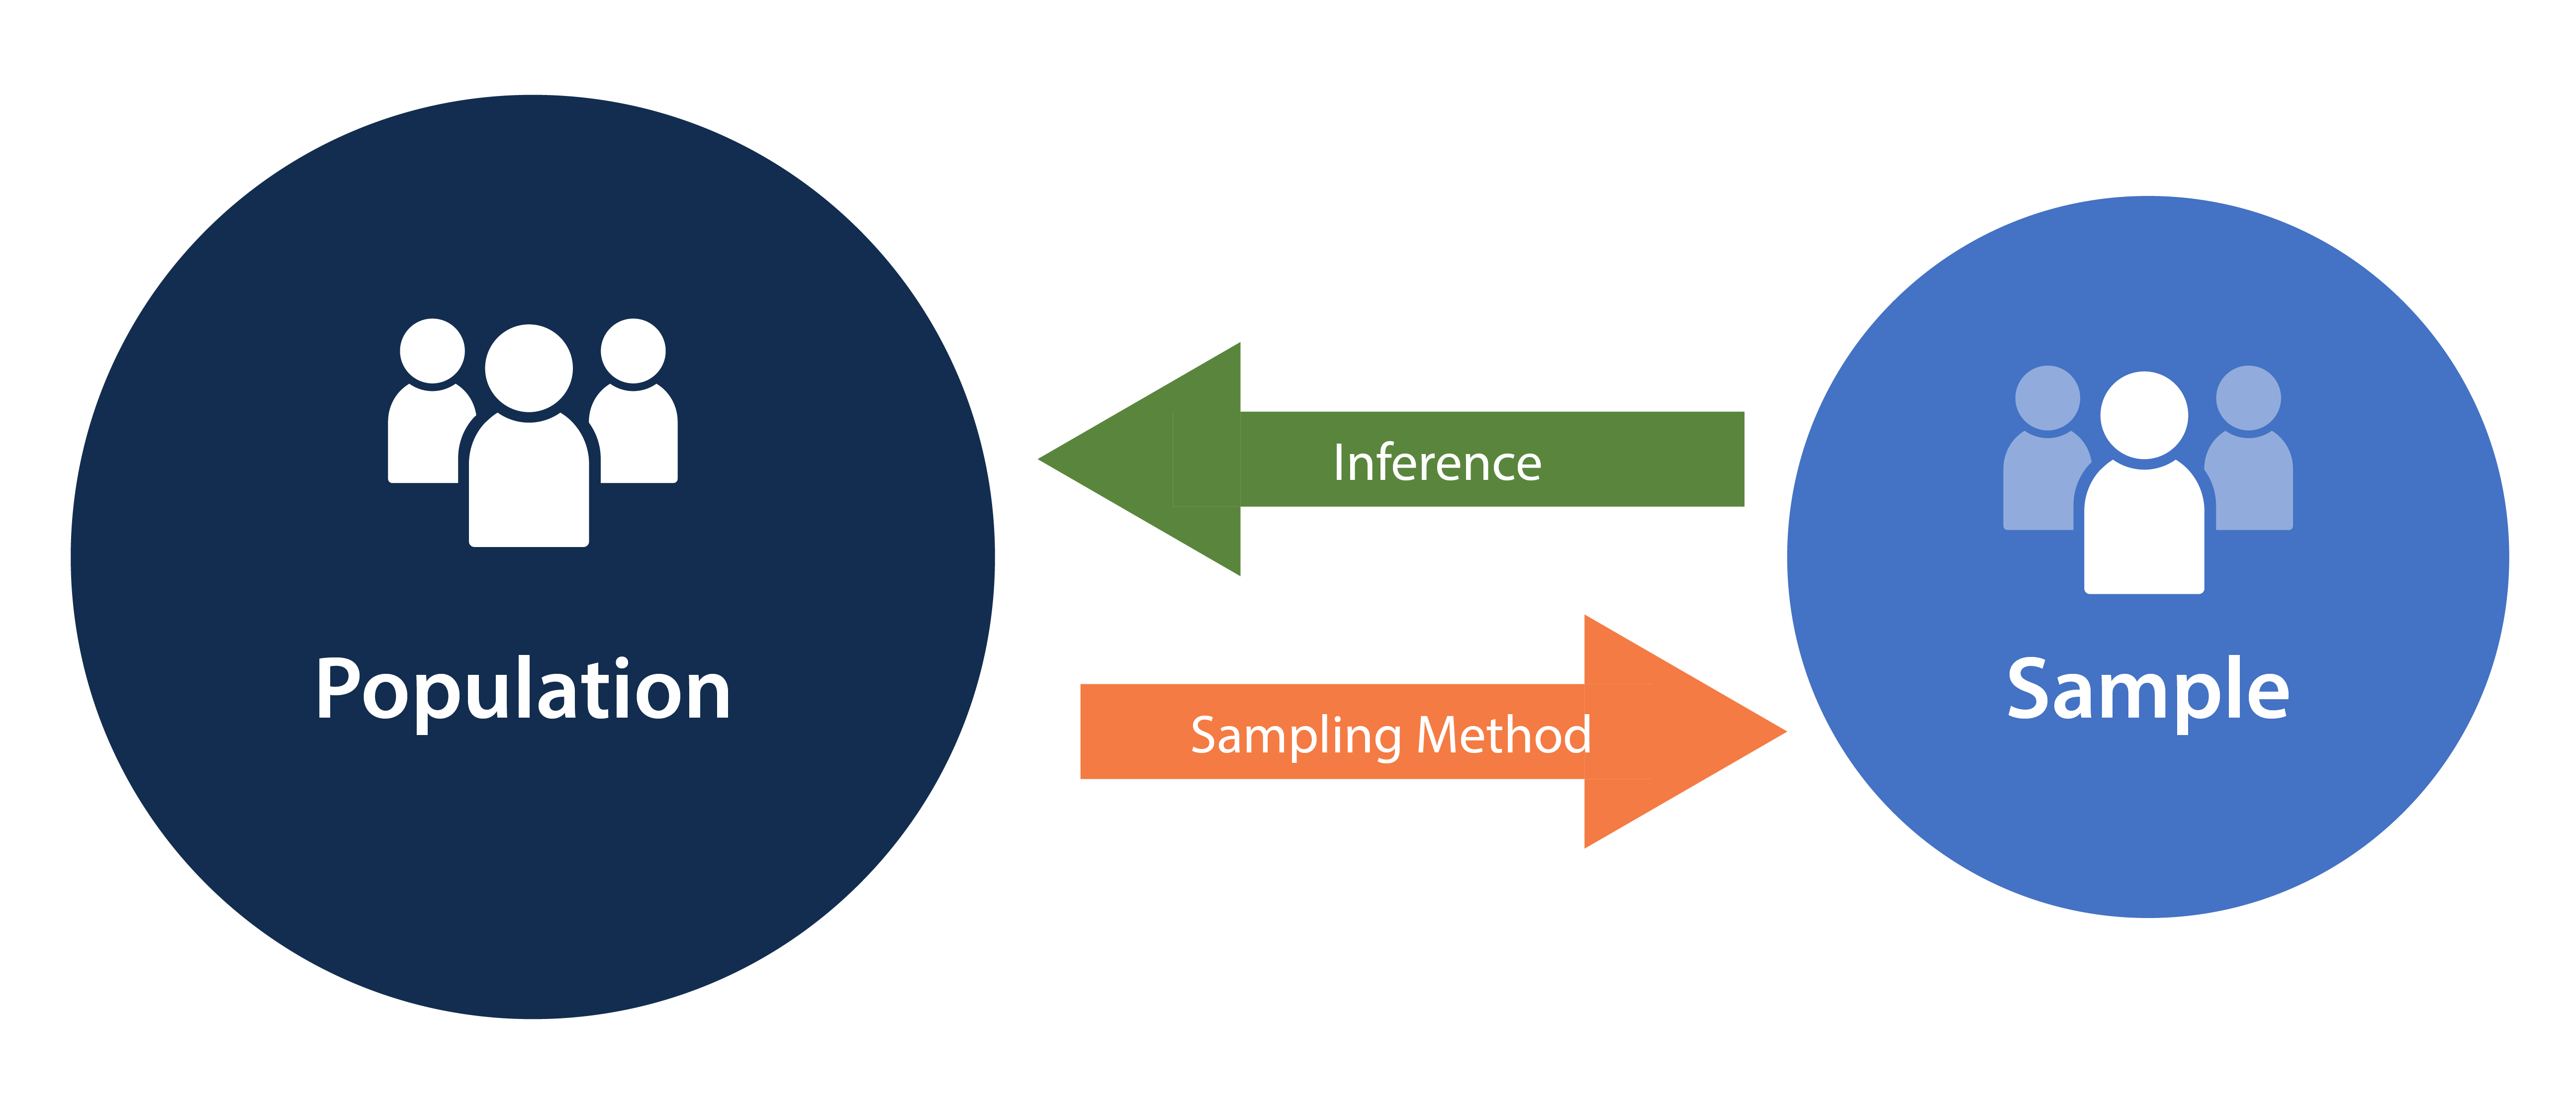
\includegraphics[
        width=0.5\linewidth,
        height=5cm,
        keepaspectratio
    ]{images/statistics/sampling-plan.png}

    \caption{Sampling Plan: Relation between Population and Sample}
\end{figure}


\begin{enumerate}
    \item \textbf{Statistical Inference}\label{Sampling Plans/Statistical Inference}: To extend your conclusions beyond the observed data.
    The field of \textbf{inferential statistics} tries to use the information from a sample to make statements or decisions about the population of interest.
    It takes into account the uncertainty that the information is coming from sampling and does not perfectly represent the population, since another sample would give different outcomes.
    An important aspect of inferential statistics is estimation of the population parameters of interest.
    \hfill \cite{statistics/book/Statistics-for-Data-Scientists/Maurits-Kaptein}

    \item Sampling procedures are formal \textit{probabilistic approaches} to help collect units from the population for the sample.
    \hfill \cite{statistics/book/Statistics-for-Data-Scientists/Maurits-Kaptein}

    \item \textbf{Population}\label{Sampling Plans/Population}: The complete set of units that we would like to say something about is called the (target) population.
    \hfill \cite{statistics/book/Statistics-for-Data-Scientists/Maurits-Kaptein}
    \\
    In principle we would expect that a population is \textbf{always finite}, since an infinite number of units does not exist in real life. However, populations are often treated as infinite. One reason is that populations can be really really large.
    \hfill \cite{statistics/book/Statistics-for-Data-Scientists/Maurits-Kaptein}
    \\
    It is mathematically often more convenient (as we will see later) to assume that such a population is infinite.
    \hfill \cite{statistics/book/Statistics-for-Data-Scientists/Maurits-Kaptein}
    \\
    Properly defining or describing a population can be difficult. Furthermore, even if the population is established, measuring all units is often impossible or too elaborate. This means that information about the population can only be obtained by considering a subset of the population.
    \hfill \cite{statistics/book/Statistics-for-Data-Scientists/Maurits-Kaptein}

    \item \textbf{Sample}\label{Sampling Plans/Sample}: The set of units for which we have obtained data is referred to as the sample.
    \hfill \cite{statistics/book/Statistics-for-Data-Scientists/Maurits-Kaptein}
    \\
    The sample is typically a subset of the population, although in theory the sample can form the whole population or the sample can contain units that are not from the target population.
    \hfill \cite{statistics/book/Statistics-for-Data-Scientists/Maurits-Kaptein}

    \item \textbf{Representative Sample}\label{Sampling Plans/Representative Sample}:  A representative sample can be intuitively defined as a sample of units that has approximately the same distribution of characteristics as the population from which it was drawn.
    \hfill \cite{statistics/book/Statistics-for-Data-Scientists/Maurits-Kaptein}
    \\
    Representative sampling is also referred to as random or probability sampling.
    \hfill \cite{statistics/book/Statistics-for-Data-Scientists/Maurits-Kaptein}

    \item \textbf{Unit}\label{Sampling Plans/Unit}: A unit is usually a concrete or physical thing for which we would like to measure its characteristics.
    \hfill \cite{statistics/book/Statistics-for-Data-Scientists/Maurits-Kaptein}

    \item \textbf{Estimates}\label{Sampling Plans/Estimates}: In terms of statistical inference, the calculations on the sample data are referred to as estimates for the theoretical value in the whole population.
    \hfill \cite{statistics/book/Statistics-for-Data-Scientists/Maurits-Kaptein}

    \item \textbf{Estimators}\label{Sampling Plans/Estimators}: quantities that we compute using the data in our sample to say something about the population.
    \hfill \cite{statistics/book/Statistics-for-Data-Scientists/Maurits-Kaptein}

    \item \textbf{Realization}\label{Sampling Plans/realization}: The values in the sample are referred to as a realization from the population.
    \hfill \cite{statistics/book/Statistics-for-Data-Scientists/Maurits-Kaptein}

    %%%%%%%%%%%%%%%%%%%%%%%%%%%%%%%%%%%%%%%%%%%%%%%%%%%%%%%%%%%%%%%%%%%%%%%%%%%%%%
    \vspace{0.5cm}

    \item Reasons for sample instead of population:
    \begin{enumerate}
        \item In many applications we really can’t measure the complete population. For instance, one of the tests applied to aircraft engines is the “frozen bird test”.
        \hfill \cite{statistics/book/Statistics-for-Data-Scientists/Maurits-Kaptein}

        \item Time, space, or budget restrictions often do not allow us to measure all units from a population.
        \hfill \cite{statistics/book/Statistics-for-Data-Scientists/Maurits-Kaptein}

        \item  Big data itself may be an argument for sampling. If we have a very large sample or we have been able to measure all units from the population, the resulting dataset can be so large that it becomes impossible to analyze the full data at one computer.
        \hfill \cite{statistics/book/Statistics-for-Data-Scientists/Maurits-Kaptein}
    \end{enumerate}

    \item A non-representative sample implies that we do not know the exact process by which units in the population became part of the sample.
    \hfill \cite{statistics/book/Statistics-for-Data-Scientists/Maurits-Kaptein}

    \item If we know which sampling procedure was applied to collect the units for the sample, we would also know how close the calculations or statistics would be to the theoretical value in the whole population.
    \hfill \cite{statistics/book/Statistics-for-Data-Scientists/Maurits-Kaptein}
    \\
    Thus the sampling procedure and the choice of calculation on the sample data (\\
    \nameref{Data/Describing Data/Central Tendency/(Arithmetic) mean or average}, \\
    \nameref{Data/Describing Data/Central Tendency/Median},\\
    \nameref{Data/Describing Data/Central Tendency/Quartiles/first quartile}, \\
    \nameref{Data/Describing Data/Central Tendency/Standard Deviation}\\
    etc.) would make statistical inference mathematically precise and it would therefore help us when making statements beyond the sample data.
    \hfill \cite{statistics/book/Statistics-for-Data-Scientists/Maurits-Kaptein}


\end{enumerate}

\section{Generic Formulation \cite{statistics/book/Statistics-for-Data-Scientists/Maurits-Kaptein}}

\begin{customArrayStretch}{1.3}
\begin{longtable}{>{\RaggedRight\arraybackslash}p{4cm} >{\centering\arraybackslash}p{0.5cm} p{10.5cm}}

\hhline{=:=:=} \endfirsthead
\hhline{=:=:=} \endhead
\hhline{=:=:=} \endfoot
\hhline{=:=:=} \endlastfoot


\textbf{Population Size} &
    $N$ &
    \hfill \cite{statistics/book/Statistics-for-Data-Scientists/Maurits-Kaptein}
    \\ \hline

\textbf{Sample Size} &
    $n$ &
    \begin{minipage}{10.3cm}
        \vspace{0.15cm}
        \begin{enumerate}
            \item $n \leq N$
            \hfill \cite{statistics/book/Statistics-for-Data-Scientists/Maurits-Kaptein}

        \end{enumerate}
        \vspace{0.15cm}
    \end{minipage}
    \\ \hline

\textbf{Number of Possible Samples} &
    $K$ &
    \begin{minipage}{10.3cm}
        \vspace{0.15cm}
        \begin{enumerate}
            \item exact value of $K$ depends on the sampling plan
            \hfill \cite{statistics/book/Statistics-for-Data-Scientists/Maurits-Kaptein}

        \end{enumerate}
        \vspace{0.15cm}
    \end{minipage}
    \\ \hline

\textbf{Population} &
    $\Omega$ &
    \begin{minipage}{10.3cm}
        \vspace{0.15cm}
        \begin{enumerate}
            \item $\Omega = \dCurlyBrac{1,2,\cdots,N}$
            \hfill \cite{statistics/book/Statistics-for-Data-Scientists/Maurits-Kaptein}

            \item $\Omega = \dbigcup_{k=1}^K S_k$
            \hfill \cite{statistics/book/Statistics-for-Data-Scientists/Maurits-Kaptein}
        \end{enumerate}
        \vspace{0.15cm}
    \end{minipage}
    \\ \hline


\textbf{Sample} &
    $S_k$ &
    \begin{minipage}{10.3cm}
        \vspace{0.15cm}
        \begin{enumerate}
            \item Subset of Population
            \hfill \cite{statistics/book/Statistics-for-Data-Scientists/Maurits-Kaptein}

            \item $k \in \dCurlyBrac{1,2,\cdots, K}$
            \hfill \cite{statistics/book/Statistics-for-Data-Scientists/Maurits-Kaptein}

            \item $S_k = \dCurlyBrac{i_1,i_2,\cdots,i_n}$  ($i_h \in \dParenBrac{1,\cdots,N}$)
            \hfill \cite{statistics/book/Statistics-for-Data-Scientists/Maurits-Kaptein}
            \\
            ($n$ unique units, $h \neq l \Rightarrow i_h \neq i_l$)
            \hfill \cite{statistics/book/Statistics-for-Data-Scientists/Maurits-Kaptein}

            \item $S_k \subset \Omega \hspace{2cm} \forall\  k \in \dParenBrac{1,\cdots,K}$
            \hfill \cite{statistics/book/Statistics-for-Data-Scientists/Maurits-Kaptein}


            \item Each subset is unique: $k\neq l \Rightarrow S_k \neq S_l$
            \hfill \cite{statistics/book/Statistics-for-Data-Scientists/Maurits-Kaptein}

            \item Subsets may overlap: $S_k \ \cap\ S_l \neq \phi$
            \hfill \cite{statistics/book/Statistics-for-Data-Scientists/Maurits-Kaptein}
        \end{enumerate}
        \vspace{0.15cm}
    \end{minipage}
    \\ \hline


\textbf{Unit} &
    $i$ &
    \hfill \cite{statistics/book/Statistics-for-Data-Scientists/Maurits-Kaptein}
    \\ \hline

\textbf{Unit's  theoretical value} &
    $x_i$ &
    \hfill \cite{statistics/book/Statistics-for-Data-Scientists/Maurits-Kaptein}
    \\ \hline

\textbf{Sample probability} &
    $\pi_k$ &
    \begin{minipage}{10.3cm}
        \vspace{0.15cm}
        \begin{enumerate}
            \item each subset $S_k$ is attached a probability $\pi_k$
            \hfill \cite{statistics/book/Statistics-for-Data-Scientists/Maurits-Kaptein}

            \item $\pi_k > 0 \hspace{2cm}  k \in \dCurlyBrac{1,\cdots,K}$
            \hfill \cite{statistics/book/Statistics-for-Data-Scientists/Maurits-Kaptein}

            \item $\dsum_{k=1}^K \pi_k = 1$
            \hfill \cite{statistics/book/Statistics-for-Data-Scientists/Maurits-Kaptein}
        \end{enumerate}
        \vspace{0.15cm}
    \end{minipage}
    \\ \hline


\textbf{Unit Probability} &
    $p_i$ &
    \begin{minipage}{10.3cm}
        \vspace{0.15cm}
        \begin{enumerate}
            \item Probability of each unit in population
            \hfill \cite{statistics/book/Statistics-for-Data-Scientists/Maurits-Kaptein}

            \item $p_i > 0 \hspace{2cm} \ i \in \dCurlyBrac{1,\cdots,N}$
            \hfill \cite{statistics/book/Statistics-for-Data-Scientists/Maurits-Kaptein}

            \item $\dsum_{i=1}^N p_i \neq 1$ since samples overlap
            \hfill \cite{statistics/book/Statistics-for-Data-Scientists/Maurits-Kaptein}

            \item the probabilities are \textbf{not} always the same for each unit.
            \hfill \cite{statistics/book/Statistics-for-Data-Scientists/Maurits-Kaptein}

        \end{enumerate}
        \vspace{0.15cm}
    \end{minipage}
    \\ \hline


\textbf{Population Parameter} &
    $\theta$ &
    \begin{minipage}{10.3cm}
        \vspace{0.15cm}
        \begin{enumerate}
            \item $\theta \equiv \theta(\mathbf{x})$ where $\mathbf{x} = \dParenBrac{x_1, x_2, \cdots, x_N}$
            \hfill \cite{statistics/book/Statistics-for-Data-Scientists/Maurits-Kaptein}

        \end{enumerate}
        \vspace{0.15cm}
    \end{minipage}
    \\ \hline


\textbf{Observations} &
    $\mathbf{x}_k^\top$ &
    \begin{minipage}{10.3cm}
        \vspace{0.15cm}
        \begin{enumerate}
            \item $\mathbf{x}_k^\top = \dParenBrac{x_{i_1}, x_{i_2}, \cdots, x_{i_n}}$
            \hfill \cite{statistics/book/Statistics-for-Data-Scientists/Maurits-Kaptein}

            \item Observed with every sample $S_k$
            \hfill \cite{statistics/book/Statistics-for-Data-Scientists/Maurits-Kaptein}
        \end{enumerate}
        \vspace{0.15cm}
    \end{minipage}
    \\ \hline

\textbf{Descriptive Statistic/ Estimate} &
    $\hat{\theta}_k$ &
    \begin{minipage}{10.3cm}
        \vspace{0.15cm}
        \begin{enumerate}
            \item $\hat{\theta}_k = T(\mathbf{x}_k)$
            \hfill \cite{statistics/book/Statistics-for-Data-Scientists/Maurits-Kaptein}

            \item Computed based on the observed data.
            \hfill \cite{statistics/book/Statistics-for-Data-Scientists/Maurits-Kaptein}

            \item used as an \textit{estimate} for the population parameter $\theta$
            \hfill \cite{statistics/book/Statistics-for-Data-Scientists/Maurits-Kaptein}

        \end{enumerate}
        \vspace{0.15cm}
    \end{minipage}
    \\ \hline

\textbf{Estimator} &
    $T(\cdot)$ &
    \begin{minipage}{10.3cm}
        \vspace{0.15cm}
        \begin{enumerate}
            \item It is a function applied to the observed data (i.e., some calculation procedure).
            \hfill \cite{statistics/book/Statistics-for-Data-Scientists/Maurits-Kaptein}

            \item In many cases the function $T$ is identical to the calculation $\theta$ at the population level, but alternative functions may be used depending on the sampling plan.
            \hfill \cite{statistics/book/Statistics-for-Data-Scientists/Maurits-Kaptein}

            \item \textbf{Example}: For estimating population mean, $\bar{x}_k$ can be used as $T$
            \hfill \cite{statistics/book/Statistics-for-Data-Scientists/Maurits-Kaptein}
        \end{enumerate}
        \vspace{0.15cm}
    \end{minipage}
    \\ \hline

\textbf{Expected Population Parameter} &
    $\mathbb{E}(T)$ &
    \begin{minipage}{10.3cm}
        \vspace{0.15cm}
        \begin{enumerate}
            \item $
                \mathbb{E}(T)
                = \dsum_{k=1}^{K} \hat{\theta}_k \pi_k
            $
            \hfill \cite{statistics/book/Statistics-for-Data-Scientists/Maurits-Kaptein}

            \item $
                \mathbb{E}(cT) = c\ \mathbb{E}(T)
                \hspace{1cm} \forall\  c \in \mbbR
            $
            \hfill \cite{statistics/book/Statistics-for-Data-Scientists/Maurits-Kaptein}

        \end{enumerate}
        \vspace{0.15cm}
    \end{minipage}
    \\ \hline


\textbf{Weighted Average} &
    $\bar{x}_{w,k}$ &
    \begin{minipage}{10.3cm}
        \vspace{0.15cm}
        \begin{enumerate}
            \item $
                \bar{x}_{w,k}
                = \dsum_{i \in S_k} w_{ik}x_i
            $
            \hfill \cite{statistics/book/Statistics-for-Data-Scientists/Maurits-Kaptein}

            \item $
                \dsum_{i \in S_k} w_{ik} = 1
            $
            \hfill \cite{statistics/book/Statistics-for-Data-Scientists/Maurits-Kaptein}

            \item If every observation has the same weight, we obtain the arithmetic average $\bar{x}_k = \dfrac{1}{n} \dsum_{i \in S_k} x_i$
            \hfill \cite{statistics/book/Statistics-for-Data-Scientists/Maurits-Kaptein}

        \end{enumerate}
        \vspace{0.15cm}
    \end{minipage}
    \\ \hline


\end{longtable}
\end{customArrayStretch}


\begin{enumerate}
    \item The set of samples $S_1, S_2,\cdots, S_K$ with their probabilities $\pi_1, \pi_2, \pi_3,\cdots,\pi_K$ is referred to as a \textbf{sampling plan}.
    \hfill \cite{statistics/book/Statistics-for-Data-Scientists/Maurits-Kaptein}

    \item The sampling plan contains all the information necessary to analyze the quality of a sampling procedure.
    \hfill \cite{statistics/book/Statistics-for-Data-Scientists/Maurits-Kaptein}

    \item \textbf{Population Mean}: \hspace{2cm} $
        \mu
        = \dfrac{1}{N}\dsum_{i=1}^N x_i
    $
    \hfill \cite{statistics/book/Statistics-for-Data-Scientists/Maurits-Kaptein}

    \item \textbf{Population Variance}: \hspace{2cm} $
        \sigma^2
        = \dfrac{1}{N}\dsum_{i=1}^N (x_i - \mu)^2
    $
    \hfill \cite{statistics/book/Statistics-for-Data-Scientists/Maurits-Kaptein}

    \item In general, the value $\hat{\theta}_k$ can be considered an estimate of the population parameter $\theta$ when sample $S_k$ would be collected.
    \hfill \cite{statistics/book/Statistics-for-Data-Scientists/Maurits-Kaptein}

    \item The estimate $\hat{\theta}_k$ will most likely be different from the population parameter $\theta$, because the sample is just a subset of the population.
    \hfill \cite{statistics/book/Statistics-for-Data-Scientists/Maurits-Kaptein}


\end{enumerate}
















\clearpage
\section{Measures of closeness}\label{Sampling Plans/Measures of closeness}


\begin{figure}[H]
    \centering
    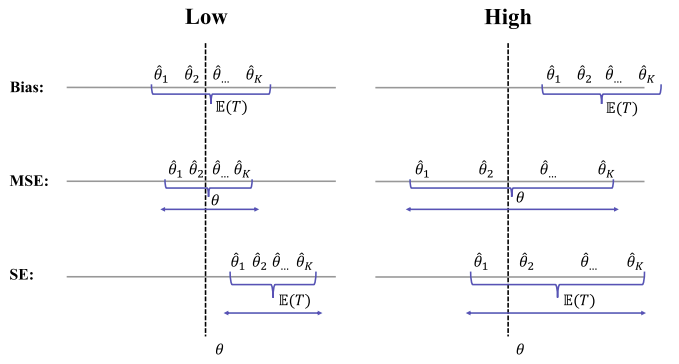
\includegraphics[
        width=0.7\linewidth,
        height=6cm,
        keepaspectratio,
    ]{images/statistics/bias-se-mse-visual.png}
    \caption{Visual Representation of Bias, MSE and SE}
\end{figure}


\subsection{Bias}\label{Sampling Plans/Measures of closeness/Bias}

\hfill
$
    bias
    = \dParenBrac{\dsum_{k=1}^{K} \hat{\theta}_k \pi_k} - \theta
    = \mathbb{E}(T) - \theta
$
\hfill \cite{statistics/book/Statistics-for-Data-Scientists/Maurits-Kaptein}

\vspace{0.5cm}

\begin{enumerate}
    \item The bias is the difference between the weighted average - over all possible $K$ samples - of the sample estimate $\hat{\theta}_k$'s and the true population parameter $\theta$.
    \hfill \cite{statistics/book/Statistics-for-Data-Scientists/Maurits-Kaptein}

    \item The weights in this weighted average are provided by the probabilities $\pi_k$.
    \hfill \cite{statistics/book/Statistics-for-Data-Scientists/Maurits-Kaptein}

    \item  If the bias of an estimator is \textbf{zero}, this means that, if we repeatedly take samples using our sampling plan and repeatedly compute our statistic of interest, the average over all of those statistics is equal to the true population parameter.
    \hfill \cite{statistics/book/Statistics-for-Data-Scientists/Maurits-Kaptein}
    \\
    If the bias is \textbf{zero}, the estimator, under the sampling plan that is being evaluated, is said to be \textbf{unbiased}.
    \hfill \cite{statistics/book/Statistics-for-Data-Scientists/Maurits-Kaptein}

    \item The bias of an estimator is thus the difference between this estimator’s expected value and the true population value.
    \hfill \cite{statistics/book/Statistics-for-Data-Scientists/Maurits-Kaptein}

    \item A small bias of an estimator under a sampling plan does \textbf{not} guarantee that individual sample results $\hat{\theta}_k$ are actually close to the population parameter $\theta$; it just states that they are close on average, if we were to sample over and over again.
    \hfill \cite{statistics/book/Statistics-for-Data-Scientists/Maurits-Kaptein}

    \item If the bias is small, $\mathbb{E}(T)$ is close to the parameter value $\theta$.\\
    If the bias is large, $\mathbb{E}(T)$ is \textbf{not} close to $\theta$
    \hfill \cite{statistics/book/Statistics-for-Data-Scientists/Maurits-Kaptein}

    \item If the sampling plan is unbiased and thus $\mathbb{E}(T) = \theta$, the RMSE and the SE are identical.
    \hfill \cite{statistics/book/Statistics-for-Data-Scientists/Maurits-Kaptein}


\end{enumerate}









\subsection{Mean Square Error (MSE)}\label{Sampling Plans/Measures of closeness/Mean Square Error (MSE)}

\hfill
$
    MSE
    = \dsum_{k=1}^{K} \dParenBrac{\hat{\theta}_k - \theta}^2 \pi_k
$
\hfill \cite{statistics/book/Statistics-for-Data-Scientists/Maurits-Kaptein}


\begin{enumerate}
    \item To capture the variability in the sample results $\hat{\theta}_1, \hat{\theta}_2,..., \hat{\theta}_K$ with respect to the true value $\theta$, we use the so-called mean squared error (MSE).
    \hfill \cite{statistics/book/Statistics-for-Data-Scientists/Maurits-Kaptein}

    \item The MSE measures the weighted average squared distance of the sample results $\hat{\theta}_1, \hat{\theta}_2,..., \hat{\theta}_K$ from the population parameter $\theta$.
    \hfill \cite{statistics/book/Statistics-for-Data-Scientists/Maurits-Kaptein}

    \item The weights are determined by the sampling probabilities.
    \hfill \cite{statistics/book/Statistics-for-Data-Scientists/Maurits-Kaptein}

    \item The smaller the MSE the better the sampling plan.
    \hfill \cite{statistics/book/Statistics-for-Data-Scientists/Maurits-Kaptein}

    \item If the MSE is small, the variability of the $\hat{\theta}_k$'s around $\theta$ is small, \\
    while if the MSE is large, the variability around $\theta$ is large.
    \hfill \cite{statistics/book/Statistics-for-Data-Scientists/Maurits-Kaptein}
\end{enumerate}







\subsection{Root Mean Square Error (RMSE)}\label{Sampling Plans/Measures of closeness/Root Mean Square Error (RMSE)}


\hfill
$
    RMSE
    = \sqrt{MSE}
    = \sqrt{{SE}^2 + \dParenBrac{\mathbb{E}(T) - \theta}^2}
$
\hfill \cite{statistics/book/Statistics-for-Data-Scientists/Maurits-Kaptein}






\subsection{Standard Error (SE)}\label{Sampling Plans/Measures of closeness/Standard Error (SE)}


\hfill
$
    SE = \sqrt{
        \dsum_{k=1}^{K} \dParenBrac{
            \hat{\theta}_k - \mathbb{E}(T)
        }^2
        \pi_k
    }
$
\hfill \cite{statistics/book/Statistics-for-Data-Scientists/Maurits-Kaptein}


\begin{enumerate}
    \item It represents the variability of the sampling plan with respect to the expected population parameter $\mathbb{E}(T)$ instead of using the true population parameter $\theta$.
    \hfill \cite{statistics/book/Statistics-for-Data-Scientists/Maurits-Kaptein}

    \item Standard error of an estimator is used as a measure to represent our uncertainty regarding an estimate.
    \hfill \cite{statistics/book/Statistics-for-Data-Scientists/Maurits-Kaptein}

    \item If the SE is small, the variability of the $\hat{\theta}_k$’s around $\mathbb{E}(T)$ is small.
    \hfill \cite{statistics/book/Statistics-for-Data-Scientists/Maurits-Kaptein}

    \item $SE(cT ) = c\ SE(T) \hspace{2cm} \forall\  c \in \mbbR$
    \hfill \cite{statistics/book/Statistics-for-Data-Scientists/Maurits-Kaptein}
\end{enumerate}








\section{Types of Samplings}

\begin{enumerate}

\item \textbf{Non-representative Sampling} \label{Sampling Plans/Non-representative Sampling}
\hfill \cite{statistics/book/Statistics-for-Data-Scientists/Maurits-Kaptein}

    \begin{enumerate}
        \item Although these sampling methods are frequently in use, it is strongly recommended not to apply these methods, unless knowledge is available on how to adjust or correct the sample for inferential purposes.
        \hfill \cite{statistics/book/Statistics-for-Data-Scientists/Maurits-Kaptein}

        \item These have the risk that some units are much more likely to be included in the sample than others, which can make statistics computed on the sample data bad estimates for the population parameters of interest.
        \hfill \cite{statistics/book/Statistics-for-Data-Scientists/Maurits-Kaptein}

        \item With non-representative sampling some units are not only more likely to be included in the sample, we also do not actually know how likely units were included.
        \hfill \cite{statistics/book/Statistics-for-Data-Scientists/Maurits-Kaptein}

        \item Even if we wanted to, we could not control for these systematic differences between units.
        \hfill \cite{statistics/book/Statistics-for-Data-Scientists/Maurits-Kaptein}
    \end{enumerate}

    \vspace{0.2cm}
    \textbf{SEE}:
    \begin{enumerate}
        \item \fullref{Sampling Plans/Non-representative Sampling/Convenience Sampling}
        \item \fullref{Sampling Plans/Non-representative Sampling/Haphazard Sampling}
        \item \fullref{Sampling Plans/Non-representative Sampling/Purposive Sampling or Judgmental Sampling}
    \end{enumerate}


\item \textbf{Representative Sampling} \label{Sampling Plans/Representative Sampling}
\hfill \cite{statistics/book/Statistics-for-Data-Scientists/Maurits-Kaptein}
    \begin{enumerate}
        \item We sample units in such a way that we do know how likely units are to be included in the sample (even if they will be different from unit to unit).
        \hfill \cite{statistics/book/Statistics-for-Data-Scientists/Maurits-Kaptein}

        \item Random sampling is a sampling method that uses a random mechanism.
        \hfill \cite{statistics/book/Statistics-for-Data-Scientists/Maurits-Kaptein}

        \begin{enumerate}
            \item The probability of each unit in the population of becoming part of the sample is both positive and known.
            \hfill \cite{statistics/book/Statistics-for-Data-Scientists/Maurits-Kaptein}
        \end{enumerate}
    \end{enumerate}

    \vspace{0.2cm}
    \textbf{SEE}:
    \begin{enumerate}
        \item \fullref{Sampling Plans/Representative Sampling/Simple Random Sampling}
        \item \fullref{Sampling Plans/Representative Sampling/Systematic Sampling}
        \item \fullref{Sampling Plans/Representative Sampling/Stratified Sampling}
        \item \fullref{Sampling Plans/Representative Sampling/Cluster Sampling}
    \end{enumerate}
\end{enumerate}

\clearpage
\section{Convenience Sampling \cite{statistics/book/Statistics-for-Data-Scientists/Maurits-Kaptein}}\label{Sampling Plans/Non-representative Sampling/Convenience Sampling}

\begin{enumerate}
    \item Convenience sampling collects only units from the population that can be easily obtained.
    \hfill \cite{statistics/book/Statistics-for-Data-Scientists/Maurits-Kaptein}

    \item This may provide a biased sample, as it represents only one small part or time window of the whole processing window for a batch of products. The term \textbf{bias}\label{Sampling Plans/Non-representative Sampling/Convenience Sampling/bias} indicates that we obtain the value of interest with a systematic mistake.
    \hfill \cite{statistics/book/Statistics-for-Data-Scientists/Maurits-Kaptein}

    \item  Convenience sampling is often justified by using the argument of population homogeneity. This insinuates that either the population units are not truly different or the process produces the population of units in random order. 
    \hfill \cite{statistics/book/Statistics-for-Data-Scientists/Maurits-Kaptein}
\end{enumerate}


\section{Haphazard Sampling \cite{statistics/book/Statistics-for-Data-Scientists/Maurits-Kaptein}}\label{Sampling Plans/Non-representative Sampling/Haphazard Sampling}

\begin{enumerate}
    \item Haphazard sampling is often believed to be an excellent way of collecting samples, because it gives a feeling or the impression that each unit was collected completely at random.
    \hfill \cite{statistics/book/Statistics-for-Data-Scientists/Maurits-Kaptein}

    \item Despite the feeling of randomness when performing haphazard sampling, often the resulting sample is not truly random.
    \hfill \cite{statistics/book/Statistics-for-Data-Scientists/Maurits-Kaptein}
\end{enumerate}

\section{Purposive Sampling/ Judgmental Sampling \cite{statistics/book/Statistics-for-Data-Scientists/Maurits-Kaptein}}\label{Sampling Plans/Non-representative Sampling/Purposive Sampling or Judgmental Sampling}

\begin{enumerate}
    \item Purposive sampling or judgmental sampling tries to sample units for a specific purpose.
    \hfill \cite{statistics/book/Statistics-for-Data-Scientists/Maurits-Kaptein}

    \item This means that the collection of units is focused on one or more particular characteristics and hence it implies that only units that are more alike are sampled.
    \hfill \cite{statistics/book/Statistics-for-Data-Scientists/Maurits-Kaptein}

    \item This way of sampling is strongly related to the definition of the population, since deliberately excluding units from the sample is analogous to limiting the population of interest.
    \hfill \cite{statistics/book/Statistics-for-Data-Scientists/Maurits-Kaptein}

    \item Purposive sampling may be useful, but it is limited since it does not allow us in general to make statements about the whole population, and at best only about a limited part of the population (although we may not be sure either).
    \hfill \cite{statistics/book/Statistics-for-Data-Scientists/Maurits-Kaptein}

    \item It does most likely produce a biased sample with respect to the complete population.
    \hfill \cite{statistics/book/Statistics-for-Data-Scientists/Maurits-Kaptein}
\end{enumerate}


\clearpage
\section{Simple Random Sampling \cite{statistics/book/Statistics-for-Data-Scientists/Maurits-Kaptein}}\label{Sampling Plans/Representative Sampling/Simple Random Sampling}

\begin{table}[H]
    \centering
    \begin{tabular}{l l}
        $N$ & population size \\
        $n$ & sample size \\
        $K$ & number of possible samples \\
        $k$ & sample index ($ k \in \dParenBrac{1,\cdots,K}$) \\
        $S_k$ & sample\\
    \end{tabular}
\end{table}

\begin{enumerate}
    \item Implicitly assume that there is no particular group structure present in the population.
    \hfill \cite{statistics/book/Statistics-for-Data-Scientists/Maurits-Kaptein}

    \item Simple random sampling is a way of collecting samples such that each unit from the population has the exact same probability of becoming part of the sample.
    \hfill \cite{statistics/book/Statistics-for-Data-Scientists/Maurits-Kaptein}


    \item Simple random sampling is a conceptually easy method of forming random samples but it can prove hard in practice.
    \hfill \cite{statistics/book/Statistics-for-Data-Scientists/Maurits-Kaptein}

    \item Simple random sampling is frequently combined with other choices or settings (see stratified and cluster sampling).
    \hfill \cite{statistics/book/Statistics-for-Data-Scientists/Maurits-Kaptein}

    \item Number of unique samples $
        = K
        = \dfrac{N!}{n!(N-n)!}
    $
    \hfill \cite{statistics/book/Statistics-for-Data-Scientists/Maurits-Kaptein}

    \item the probability of collecting sample $S_k$, using sequential sampling $
        = \dfrac{1}{K}
        = \dfrac{n!(N-n)!}{N!}
    $
    \hfill \cite{statistics/book/Statistics-for-Data-Scientists/Maurits-Kaptein}

    \item The probability that a specific unit is part of the sample $
        = \dfrac{n}{N}
    $
    \hfill \cite{statistics/book/Statistics-for-Data-Scientists/Maurits-Kaptein}

    \item The probability that a specific unit is \textbf{not} contained in the sample $
        = 1 - \dfrac{n}{N}
        = \dfrac{N-n}{N}
    $
    \hfill \cite{statistics/book/Statistics-for-Data-Scientists/Maurits-Kaptein}

    \item The number of samples that does \textbf{not} contain a specific unit $
        = \dfrac{(N - 1)!}{n!(N - 1 - n)!}
    $
    \hfill \cite{statistics/book/Statistics-for-Data-Scientists/Maurits-Kaptein}

    \item Number of samples that contain certain unit $i$ = $\dfrac{nK}{N}$
    \hfill \cite{statistics/book/Statistics-for-Data-Scientists/Maurits-Kaptein}
    \\
    $
        \Rightarrow
        \dsum_{k=1}^{K}\ \dsum_{i \in S_k} x_i
        = \dfrac{nK}{N}\dsum_{i=1}^{N} x_i
    $
    \hfill \cite{statistics/book/Statistics-for-Data-Scientists/Maurits-Kaptein}

    \item Population Variance: $
        \sigma^2
        = \dfrac{1}{N} \dsum_{i=1}^N (x_i-\mu)^2
    $
    \hfill \cite{statistics/book/Statistics-for-Data-Scientists/Maurits-Kaptein}

    \item \textbf{Disadvantage}: When the numbers of units across these subpopulations are (substantially) different, simple random may not collect units from each subgroup.
    \hfill \cite{statistics/book/Statistics-for-Data-Scientists/Maurits-Kaptein}

\end{enumerate}

\vspace{0.5cm}
\textbf{Example}:
\begin{enumerate}
    \item[] $N = 20,\ n = 5$

    \item[] $K = \dfrac{20!}{5!\cdot 15!}=15504$


\end{enumerate}


\subsection{Estimation for population mean}
\begin{enumerate}
    \item Estimator: $
        T
        = \bar{x}
        = \dfrac{1}{n} \dsum_{i=1}^n x_i
    $
    \hfill \cite{statistics/book/Statistics-for-Data-Scientists/Maurits-Kaptein}

    \item Bias: $0$
    \hfill \cite{statistics/book/Statistics-for-Data-Scientists/Maurits-Kaptein}

    \item $
        MSE(\bar{x}_k)
        = \dfrac{\sigma^2 }{n}
        \dParenBrac{\dfrac{N}{N-1}}
        \dParenBrac{1-\dfrac{n}{N}}
        = \dfrac{\sigma^2\ (N-n)}{n\ (N-1)}
    $
    \hfill \cite{statistics/book/Statistics-for-Data-Scientists/Maurits-Kaptein}
    \\
    MSE shows that it becomes equal to zero when the sample size $n$ becomes equal to the population size $N$.
    \hfill \cite{statistics/book/Statistics-for-Data-Scientists/Maurits-Kaptein}
    \\
    The MSE will not become zero when the estimator is biased, even if the sample size is equal to the population size.
    \hfill \cite{statistics/book/Statistics-for-Data-Scientists/Maurits-Kaptein}


    \item $
        \mathbb{E}[T]
        = \dfrac{1}{K}\dsum_{k=1}^{K} \bar{x}_k
        = \dfrac{1}{nK}\dsum_{k=1}^{K}\ \dsum_{i \in S_k} x_i
        = \dfrac{1}{N}\dsum_{i=1}^{N} x_i
        = \mu
    $
    \hfill \cite{statistics/book/Statistics-for-Data-Scientists/Maurits-Kaptein}
\end{enumerate}


\subsection{Estimation of the sample MSE}

\begin{enumerate}
    \item unbiased estimator for $\sigma^2$: \\
    $
       \hat{\sigma}^2 = \dfrac{N - 1}{N}\ s^2_k
    $
    \hfill
    $
        \dParenBrac{\
            s^2_k = \dfrac{1}{n - 1} \dsum_{i\ \in\ S_k} (x_i - \bar{x}_k )^2
        \ }
    $
    \hfill \cite{statistics/book/Statistics-for-Data-Scientists/Maurits-Kaptein}

    \item $
        \hat{MSE}(\bar{x}_k)
        = \dfrac{N - n}{N n}\ s^2_k
    $
    \hfill \cite{statistics/book/Statistics-for-Data-Scientists/Maurits-Kaptein}

    \item This is an unbiased estimator of the MSE of the arithmetic average in $MSE(\bar{x}_k)$ and it may also be used when the observations are binary.
    \hfill \cite{statistics/book/Statistics-for-Data-Scientists/Maurits-Kaptein}


\end{enumerate}




\subsection{Sample Statistics ($T_n$)}

\begin{enumerate}
    \item We can view a sample $X_1 , X_2 , \cdots, X _n$ of size $n$ from a population as a set of random variables (and $x_1 , x_2, \cdots , x _n$ as the set of realizations) all coming from the same distribution function $F$.
    Let $X_1 , X_2, \cdots , X _n$ be i.i.d. with $X _i \sim F$
    \hfill \cite{statistics/book/Statistics-for-Data-Scientists/Maurits-Kaptein}

    \item A sample statistic $T_n \in \mbbR$ is now defined as any function $T_n \equiv T (X_1, X_2, \cdots , X _n )$ that is applied to the sample $X_1 , X_2, \cdots , X _n$.
    As $T_n$ is a function of random variables, it is itself a random variable.
    \hfill \cite{statistics/book/Statistics-for-Data-Scientists/Maurits-Kaptein}

    \item realization for the sample statistic $T_n$: $t _n = T (x_1, x_2, \cdots , x _n )$
    \hfill \cite{statistics/book/Statistics-for-Data-Scientists/Maurits-Kaptein}

    \item \textbf{Sample average}: $T_n = \bar{X} = \dfrac{1}{n}\dsum^n _{i=1} X _i$
    \hfill \cite{statistics/book/Statistics-for-Data-Scientists/Maurits-Kaptein}

    \item \textbf{Sample variance}: $T_n = S^2 = \dfrac{1}{n - 1} \dsum^n _{i=1}(X _i - \bar{X})^2$
    \hfill \cite{statistics/book/Statistics-for-Data-Scientists/Maurits-Kaptein}

    \item \textbf{Sample standard deviation}: $T_n = S^2 = \sqrt{\dfrac{1}{n - 1} \dsum^n _{i=1}(X _i - \bar{X})^2}$
    \hfill \cite{statistics/book/Statistics-for-Data-Scientists/Maurits-Kaptein}

    \item \textbf{Sample skewness}: $T_n = b_1 = \dfrac{1}{n S^3} \dsum^n _{i=1} (X _i - \bar{X})^3$
    \hfill \cite{statistics/book/Statistics-for-Data-Scientists/Maurits-Kaptein}

    \item \textbf{Sample excess kurtosis}: $T_n = b_2 = \dParenBrac{\dfrac{1}{n S^4} \dsum^n _{i=1} (X _i - \bar{X})^4} - 3$
    \hfill \cite{statistics/book/Statistics-for-Data-Scientists/Maurits-Kaptein}

    \item \textbf{Sample minimum}: $T_n = X_{(1)} = \min \dCurlyBrac{X_1, X_2, \cdots, X _n }$
    \hfill \cite{statistics/book/Statistics-for-Data-Scientists/Maurits-Kaptein}

    \item \textbf{Sample maximum}: $T_n = X_{(n)} = \max \dCurlyBrac{X_1, X_2, \cdots, X _n }$
    \hfill \cite{statistics/book/Statistics-for-Data-Scientists/Maurits-Kaptein}

    \item \textbf{quantile}:
    \begin{enumerate}
        \item If $np \in \mathbb{N}$ is an integer, the quantile $x _p$ is estimated by the average of two sequential order statistics: $q _p = \dfrac{[X_{(np)} + X_{(1+np)}]}{2}$.
        \hfill \cite{statistics/book/Statistics-for-Data-Scientists/Maurits-Kaptein}

        \item If $np \notin \mathbb{N}$ is not an integer, we take the smallest integer value that is larger than or equal to $np$, which is denoted by $\dceil{np}$.
        \hfill \cite{statistics/book/Statistics-for-Data-Scientists/Maurits-Kaptein}
    \end{enumerate}
\end{enumerate}




\clearpage
\section{Systematic Sampling \cite{statistics/book/Statistics-for-Data-Scientists/Maurits-Kaptein}}\label{Sampling Plans/Representative Sampling/Systematic Sampling}

\begin{table}[H]
    \centering
    \begin{tabular}{l l l}
        $N$ & population size & $N=nm$\\
        $n$ & number of groups & = sample size \\
        $m$ & number of units in each group & = number of possible samples\\
        $k$ & sample index & $k \in \dParenBrac{1,\cdots,m}$ \\
        $S_k$ & sample & \\
    \end{tabular}
\end{table}

\begin{enumerate}
    \item Implicitly assume that there is no particular group structure present in the population.
    \hfill \cite{statistics/book/Statistics-for-Data-Scientists/Maurits-Kaptein}

    \item Steps:
    \hfill \cite{statistics/book/Statistics-for-Data-Scientists/Maurits-Kaptein}
    \begin{enumerate}
        \item First the population should be divided into $n$ groups and the order of the units (if Some order exists) should be maintained (or otherwise fix the order).\\
        Each group consists of $m$ units ordered from $1$ to $m$ in each group.

        \item Collect $p$th unit ($p \in \dParenBrac{1,\cdots,m}$) from all $n$ groups with probability of $\dfrac{1}{m}$\\
        (each unit in the population still has the same probability of being collected)\\
        $S_k = \dCurlyBrac{k, k + m, k + 2m, \cdots , k + (n - 1)m}$ 
        \hfill
        (Total units collected $= n$) 
        \hfill \cite{statistics/book/Statistics-for-Data-Scientists/Maurits-Kaptein} \\
        So, total number of samples $= m$ only

    \end{enumerate}

    \item The possible samples from systematic sampling are quite different from the set of samples that can be obtained with simple random sampling.
    \hfill \cite{statistics/book/Statistics-for-Data-Scientists/Maurits-Kaptein}

    \item population mean: $
        \mu 
        = \dfrac{1}{N}\ \dsum^m_{h=1} \ \dsum^n_{i=1} x_{\ k+m(i-1)}
    $
    \hfill \cite{statistics/book/Statistics-for-Data-Scientists/Maurits-Kaptein}

    \item population variance: $
        \sigma^2 
        = \dfrac{1}{N}\ \dsum^m_{k=1} \ \dsum^n_{i=1} (x_{\ k+m(i-1)} - \mu)^2
    $
    \hfill \cite{statistics/book/Statistics-for-Data-Scientists/Maurits-Kaptein}
    
    \item sample average for sample $S_k$: $
        \bar{x}_k 
        = \dfrac{1}{n}\ \dsum^n_{i=1} x_{\ k+m(i-1)}
    $
    \hfill \cite{statistics/book/Statistics-for-Data-Scientists/Maurits-Kaptein}

    \item Systematic sampling can be more efficient than simple random sampling, in particular when the variance in the systematic samples is larger than the population variance (which is impossible to verify in practice).
    \hfill \cite{statistics/book/Statistics-for-Data-Scientists/Maurits-Kaptein}

    \item The most important \textbf{advantage} of systematic sampling over simple random sampling is the ease with which the sample may be collected.
    \hfill \cite{statistics/book/Statistics-for-Data-Scientists/Maurits-Kaptein}

    \item A clear \textbf{disadvantage} of systematic sampling is that the “period” for systematic sampling may coincide with particular patterns in the process or population.
    \hfill \cite{statistics/book/Statistics-for-Data-Scientists/Maurits-Kaptein}

    \item \textbf{Disadvantage}: When the numbers of units across these subpopulations are (substantially) different, systematic sampling may not collect units from each subgroup.
    \hfill \cite{statistics/book/Statistics-for-Data-Scientists/Maurits-Kaptein}

    \item TODO? Systematic Sampling samples ($S_1,\cdots,S_m$) are subset of Simple Random Sampling samples ($S_1,\cdots,S_K$).
\end{enumerate}

\vspace{0.5cm}
\textbf{Example}:
\begin{enumerate}
    \item[] $N = 20,\ n = 5$

    \item[] $m = \dfrac{20}{5}=4$

    
\end{enumerate}



\subsection{Estimation for population mean}
\begin{enumerate}
    \item Estimator: $
        \dfrac{1}{n} \dsum_{i=1}^n x_i
    $
    \hfill \cite{statistics/book/Statistics-for-Data-Scientists/Maurits-Kaptein}
    \\
    if population can be perfectly split up into $n$ groups of $m$ units:\\
    Unbiased Estimator: $\bar{x}_k$
    
    \item Bias: $0$
    \hfill \cite{statistics/book/Statistics-for-Data-Scientists/Maurits-Kaptein}

    \item MSE: $
        \sigma^2 -
        \dfrac{1}{N}
        \dsum_{h=1}^{n}
        \dsum_{i=1}^{m}
        (x_{h+m(i-1)} - \bar{x}_h)^2
    $
    \hfill \cite{statistics/book/Statistics-for-Data-Scientists/Maurits-Kaptein}

\end{enumerate}



\subsection{Estimation of the MSE}

\begin{enumerate}
    \item In the general setting for systematic sampling, an unbiased estimation of the MSE is \textbf{not possible}.
    \hfill \cite{statistics/book/Statistics-for-Data-Scientists/Maurits-Kaptein}

    \item Given that there is no systematic difference between units based on their position in the groups (and the ratio of sample and population size is an integer), the MSE of the sample average under systematic sampling becomes equal to the MSE of the sample average under simple random sampling.
    \hfill \cite{statistics/book/Statistics-for-Data-Scientists/Maurits-Kaptein}
    
    \item unbiased estimator: $
        \dfrac{N - 1}{N}\ s^2_k
    $
    \hfill
    $
        s^2_k = \dfrac{1}{n - 1} \dsum^n_{i=1} (x_{k+m(i-1)} - \bar{x}_k )^2
    $
    \hfill \cite{statistics/book/Statistics-for-Data-Scientists/Maurits-Kaptein}
\end{enumerate}






\clearpage
\section{Stratified Sampling \cite{statistics/book/Statistics-for-Data-Scientists/Maurits-Kaptein}}\label{Sampling Plans/Representative Sampling/Stratified Sampling}

\begin{customArrayStretch}{1.3}
\begin{longtable}{>{\centering\arraybackslash}p{1.5cm} p{9cm} p{3.5cm}}

\hline\endfirsthead
\hline\endhead
\hline\endfoot
\hline\endlastfoot

$N$ & total population size & \\ \hline

$n$ & total sample size & \\ \hline

$M$ & number of sub-populations & \\ \hline

$N_h$ & $k$th sub-population size & $\tsum_{h=1}^{M} N_h = N$ \\ \hline

$n_h$ & sample size from $k$th sub-population & $\tsum_{h=1}^{M} n_h = n$ \\ \hline

$h$ & Stratum index & $h \in \dCurlyBrac{1, \cdots, M}$ \\ \hline

$k$ & Stratum index & $k \in \dCurlyBrac{1, \cdots, K_S}$ \\ \hline

$K_h$ & The number of possible samples that can be drawn from stratum $h$ \\ \hline

$K_S$ & total number of possible samples \\ \hline

$(h, i)$ & index of unit & \begin{minipage}{3.2cm}
    \vspace{0.1cm}
    $i \in \dCurlyBrac{1, 2,\cdots, N_h }$ \\
    and $h \in \dCurlyBrac{1, 2,..., M}$
    \vspace{0.1cm}
\end{minipage}  \\ \hline

$x_{hi}$ & unit $i$ in stratum $h$ \\ \hline

$w_{h}$ &
    weight of strata $h$ while sampling &
    \begin{minipage}{3.2cm}
        \vspace{0.1cm}
        $w_{h} = \dfrac{N_h}{N}$
        \vspace{0.1cm}
    \end{minipage}
    \\ \hline

$f_{h}$ &
    sample fraction in stratum $h$ &
    \begin{minipage}{3.2cm}
        \vspace{0.1cm}
        $f_{h} = \dfrac{n_h}{N_h}$
        \vspace{0.1cm}
    \end{minipage}
    \\ \hline

$S_{h,k}$ &
\multicolumn{2}{l}{
    \begin{minipage}{11cm}
        \vspace{0.1cm}
        $S_{h,k}$ is the collected sample in stratum $h$ \\
        The $k$-th possible sample from stratum $h$ \\
        (e.g., $S_{2,3}$ is the $3$rd possible sample from stratum $2$) \\
        focuses on one stratum
        \vspace{0.1cm}
    \end{minipage}
} \\ \hline

$S_k$ &
\multicolumn{2}{l}{
    \begin{minipage}{11cm}
        \vspace{0.1cm}
        The $k$-th possible full stratified sample (i.e., across all strata). \\
        Each $S_k$ includes one selected sample from each stratum.\\
        focuses on a complete sample (all strata combined)
        \vspace{0.1cm}
    \end{minipage}
} \\ \hline

\end{longtable}
\end{customArrayStretch}

\begin{enumerate}
    \item Stratified sampling is used to accommodate the issue of missing out on sub-populations during sampling by setting the sample size for each subpopulation (often called \textbf{strata}\label{Sampling Plans/Representative Sampling/Stratified Sampling/strata}) to a fixed percentage of the number of units of the subpopulation.
    \hfill \cite{statistics/book/Statistics-for-Data-Scientists/Maurits-Kaptein}

    \item Steps:
    \hfill \cite{statistics/book/Statistics-for-Data-Scientists/Maurits-Kaptein}
    \begin{enumerate}
        \item The population is then divided into $n$ groups such that the order in units is maintained.

        \item From $k$th group/ strata one unit is randomly collected with probability $\dfrac{n_h}{N_h}$, when each group contains $n_h$ units.\\
        Unlike systematic sampling, random unit is collected instead of $p$th unit.
    \end{enumerate}

    \item This form of stratified sampling is not identical to systematic sampling (although this method of stratified sampling is sometimes referred to as systematic sampling).
    \hfill \cite{statistics/book/Statistics-for-Data-Scientists/Maurits-Kaptein}

    \item Stratified sampling may lead to samples that are not possible with systematic sampling, but it does not produce all possible samples from simple random sampling.
    \hfill \cite{statistics/book/Statistics-for-Data-Scientists/Maurits-Kaptein}

    \item $
        K_h = \binom{N_h}{n_h} = \dfrac{N_h!}{n_h!(N_h-n_h)!}
    $
    \hfill \cite{statistics/book/Statistics-for-Data-Scientists/Maurits-Kaptein}

    \item The number of possible samples: $
        K_S
        = \dprod_{h=1}^{M} \dfrac{N_h!}{n_h!(N_h-n_h)!}
        = \dprod_{h=1}^{M} K_h
    $
    \hfill \cite{statistics/book/Statistics-for-Data-Scientists/Maurits-Kaptein}

    \item The probability of collecting any of the $K_S$ samples $
        = \dfrac{1}{K_S}
    $
    \hfill \cite{statistics/book/Statistics-for-Data-Scientists/Maurits-Kaptein}

    \item The probability of collecting a unit now depends on the stratum the unit is part of.
    \hfill \cite{statistics/book/Statistics-for-Data-Scientists/Maurits-Kaptein}

    \item If $
        \dfrac{n_i}{N_i} = \dfrac{n_j}{N_j}
        \hspace{0.3cm}
        \forall
        \hspace{0.3cm}
        i,j \in \dParenBrac{1,\cdots,M}
    $, then its called \textbf{Proportional Stratified Sampling}.\label{Sampling Plans/Representative Sampling/Stratified Sampling/Proportional Stratified Sampling}
    \hfill \cite{statistics/book/Statistics-for-Data-Scientists/Maurits-Kaptein}

\end{enumerate}


\vspace{0.5cm}\hspace{0cm}
\textbf{Example}: sample $10\%$ from each sub-population


\subsection{population stratum}
\begin{enumerate}
    \item population stratum mean: $
        \mu_h = \dfrac{1}{N_h} \ \dsum_{i=1}^{N_h} \ x_{hi}
    $
    \hfill \cite{statistics/book/Statistics-for-Data-Scientists/Maurits-Kaptein}

    \item population stratum variance: $
        \sigma^2_h = \dfrac{1}{N_h} \ \dsum_{i=1}^{N_h} \ (x_{hi} - \mu_h)^2
    $
    \hfill \cite{statistics/book/Statistics-for-Data-Scientists/Maurits-Kaptein}

\end{enumerate}



\subsection{population}
\begin{enumerate}
    \item population mean: $
        \mu
        = \dfrac{1}{N} \ \dsum_{h=1}^M \ \dsum_{i=1}^n\  x_{hi}
        = \dsum_{h=1}^M \ w_h\mu_h
    $
    \hfill \cite{statistics/book/Statistics-for-Data-Scientists/Maurits-Kaptein}
    \begin{enumerate}
        \item $w_h = \dfrac{N_h}{N}$
        \hfill \cite{statistics/book/Statistics-for-Data-Scientists/Maurits-Kaptein}

        \item $\dsum_{h=1}^M \ w_h = 1$
        \hfill \cite{statistics/book/Statistics-for-Data-Scientists/Maurits-Kaptein}
    \end{enumerate}


    \item population variance: $
        \sigma^2
        \equiv \dfrac{1}{N} \ \dsum_{h=1}^M \ \dsum_{i=1}^{N_h} (x_{hi} - \mu)^2
        = \dsum_{h=1}^M w_h \sigma_h^2 + \dsum_{h=1}^M w_h (\mu_h - \mu)^2
    $
    \hfill \cite{statistics/book/Statistics-for-Data-Scientists/Maurits-Kaptein}
    \vspace{0.15cm}
    \begin{enumerate}
        \item \textbf{within (strata) variances}: the first part represents a weighted mean of the within strata variances

        \item \textbf{between (strata) variances}: the second part represents a weighted mean of the squared distances of the strata means to the population mean
    \end{enumerate}

\end{enumerate}


\subsubsection{Estimation for population mean}
\begin{enumerate}
    \item Estimator: $
        \dsum_{h=1}^{M}
        \dfrac{N_h}{N}
        \dParenBrac{\dfrac{1}{n_h} \dsum_{i=1}^{n_h} x_{hi}}
        =
        \dsum_{h=1}^{M} \ w_h \ \bar{x}_{h,k}
    $
    \hfill \cite{statistics/book/Statistics-for-Data-Scientists/Maurits-Kaptein}

    \item Bias: $0$
    \hfill \cite{statistics/book/Statistics-for-Data-Scientists/Maurits-Kaptein}

    \item MSE: $
        \dsum_{h=1}^{M}
        \dSquareBrac{
            \dParenBrac{
                \dfrac{
                    N_h^2\ (N_h - n_h)
                }{
                    n_h\ (N_h-1)\ N^2
                }
            } \sigma_h^2
        }
    $
    \hfill \cite{statistics/book/Statistics-for-Data-Scientists/Maurits-Kaptein}
\end{enumerate}




\subsection{sample stratum}
\begin{enumerate}
    \item sample stratum mean: $
        \bar{x}_{h,k} = \dfrac{1}{n_h} \ \dsum_{i \ \in \ S_{h,k}} \ x_{hi}
    $
    \hfill \cite{statistics/book/Statistics-for-Data-Scientists/Maurits-Kaptein}

    \item sample stratum variance: $
        s^2_{h,k} = \dfrac{1}{n_h-1} \ \dsum_{i \ \in \ S_{h,k}} \ (x_{hi} - \bar{x}_{h,k})^2
    $
    \hfill \cite{statistics/book/Statistics-for-Data-Scientists/Maurits-Kaptein}

    \item MSE for unbiased estimator:
    $
        MSE(\bar{x}_{h,k}) = \tVar[\bar{x}_{h,k}] = SE^2(\bar{x}_{h,k})
    $
    \hfill \cite{common/online/chatgpt}

    \item The bias and standard error within each stratum $h$ now follow the theory of simple random sampling.
    \hfill \cite{statistics/book/Statistics-for-Data-Scientists/Maurits-Kaptein}

    \item bias of $\bar{x}_{h,k}$ = 0 in stratum $h$ is zero for the stratum mean $\mu_h$

\end{enumerate}


\subsubsection{Estimation for sample stratum SE}
\begin{enumerate}
    \item $
        \hat{SE}(\bar{x}_{h,k})
        = \sqrt{\dfrac{1 - f_h}{n_h}} s_{h,k}
    $
    \hfill
    $f_h = \dfrac{n_h}{N_h}$
    \hfill \cite{statistics/book/Statistics-for-Data-Scientists/Maurits-Kaptein}
\end{enumerate}



\subsection{sample}
\begin{enumerate}
    \item Sample average: $
        \bar{x}_k = \dsum^M_{h=1} w_h\ \bar{x}_{h,k}
    $
    \hfill \cite{statistics/book/Statistics-for-Data-Scientists/Maurits-Kaptein}

    \item the \textit{simple random samples} from the different strata are completely \textbf{unrelated}, which implies that the sum of the squared standard errors of $w_h \ \bar{x}_{h,k}$ form the squared standard error of the sample average $\bar{x}_k$.
    \hfill \cite{statistics/book/Statistics-for-Data-Scientists/Maurits-Kaptein}
    \\
    $
        \tVar[\bar{x}_k] = \dsum_{h=1}^M w_h^2 \cdot \tVar[\bar{x}_{h,k}]
    $
    \hfill \cite{common/online/chatgpt}


    \item squared standard error of $\bar{x}_k$:
    $
        SE^2(\bar{x}_k) = \dsum_{h=1}^M w_h^2 \cdot SE^2(\bar{x}_{h,k})
    $
    \hfill \cite{common/online/chatgpt}

    \item $
        MSE(\bar{x}_k )
        = \dsum^M_{h=1} w^2_h \cdot MSE(\bar{x}_{h,k} )
        = \dsum^M_{h=1} \dfrac{N_h}{(N_h - 1)n_h} \ (1 - f_h)\ w^2_h\ \sigma^2_h$
    \hfill \cite{statistics/book/Statistics-for-Data-Scientists/Maurits-Kaptein}

\end{enumerate}


\subsubsection{Estimation of the sample MSE}

$
    \hat{MSE} (\bar{x}_k )
    = \dsum^M_{h=1} \dfrac{1 - f_h}{n_h} \ w^2_h\ s^2_{h,k}.
$
\hfill \cite{statistics/book/Statistics-for-Data-Scientists/Maurits-Kaptein}

SEE: \url{https://chatgpt.com/share/680251af-c100-800a-a533-c26a0001b651}

\subsubsection{Estimation of the sample SE}

An estimate of the standard error of $\bar{x}_k$ is now obtained by taking the square root of
the estimated MSE:
\hfill \cite{statistics/book/Statistics-for-Data-Scientists/Maurits-Kaptein}
\\
$
    \hat{SE}(\bar{x}_k) = \sqrt{\hat{MSE} (\bar{x}_k )}
$














\clearpage
\section{Cluster Sampling \cite{statistics/book/Statistics-for-Data-Scientists/Maurits-Kaptein}}\label{Sampling Plans/Representative Sampling/Cluster Sampling}

\begin{enumerate}[itemsep=0.2cm]
    \item Cluster sampling involves random sampling of groups or clusters of units in the population.
    \hfill \cite{statistics/book/Statistics-for-Data-Scientists/Maurits-Kaptein}

    \item Cluster sampling can be less representative than sampling units directly.
    \hfill \cite{statistics/book/Statistics-for-Data-Scientists/Maurits-Kaptein}

    \item Cluster sampling introduces a specific structure in the sample which should also be addressed when the data is being analyzed. 
    \hfill \cite{statistics/book/Statistics-for-Data-Scientists/Maurits-Kaptein}
    
    \item The cluster structure introduces two sources of variation in the data being collected. These sources of variation need to be quantified to make proper statements on the population of interest.
    \hfill \cite{statistics/book/Statistics-for-Data-Scientists/Maurits-Kaptein}
    \begin{enumerate}[itemsep=0.1cm]
        \item \textbf{Within-Cluster Variation}:\label{Sampling Plans/Representative Sampling/Cluster Sampling/Within-Cluster Variation}
        \hfill \cite{common/online/chatgpt}
        \begin{enumerate}
            \item This refers to the differences among units within the same cluster.
            \hfill \cite{common/online/chatgpt}

            \item This variation is often smaller compared to between-cluster variation because individuals within a cluster tend to be more similar.
            \hfill \cite{common/online/chatgpt}

        \end{enumerate}

        \item \textbf{Between-Cluster Variation}:\label{Sampling Plans/Representative Sampling/Cluster Sampling/Between-Cluster Variation}
        \hfill \cite{common/online/chatgpt}
        \begin{enumerate}
            \item This refers to the differences between clusters.
            \hfill \cite{common/online/chatgpt}

            \item This variation is often larger in cluster sampling because different clusters may have distinct characteristics.
            \hfill \cite{common/online/chatgpt}

        \end{enumerate}
        
    \end{enumerate}

    \item The sampling units for the \textit{first stage} are referred to as \textbf{primary cluster units}\label{Sampling Plans/Representative Sampling/Cluster Sampling/primary cluster units}.
    \hfill \cite{statistics/book/Statistics-for-Data-Scientists/Maurits-Kaptein}

    \item Sampling these different levels of clusters can be performed using simple random sampling, systematic sampling, or even stratified sampling, if certain cluster are put together on certain criteria.
    \hfill \cite{statistics/book/Statistics-for-Data-Scientists/Maurits-Kaptein}

    \item Cluster sampling is in a way related to stratified sampling (clusters may be viewed as strata).
    \hfill \cite{statistics/book/Statistics-for-Data-Scientists/Maurits-Kaptein}

    \item Since we deal with multiple levels of hierarchical clusters, the calculation of the probability of collecting one unit from the population and the probability of collecting one of the many sample sets are complex.
    \hfill \cite{statistics/book/Statistics-for-Data-Scientists/Maurits-Kaptein}
\end{enumerate}




\subsection{Single-Stage Cluster Sampling}\label{Sampling Plans/Representative Sampling/Cluster Sampling/Single-Stage Cluster Sampling}

A single-stage cluster sample uses a random sample of the clusters and then all units from these clusters are selected. 
\hfill \cite{statistics/book/Statistics-for-Data-Scientists/Maurits-Kaptein}

\subsubsection{cluster sizes are not all equal}
    
Estimator for population mean: $
    \dsum_{h=1}^{m}
    \dParenBrac{
        \dfrac{N_h}{
            \tsum_{h=1}^{m} N_h
        }
    }
    \bar{x}_h
$
\hfill \cite{statistics/book/Statistics-for-Data-Scientists/Maurits-Kaptein}

\begin{enumerate}[itemsep=0.25cm]
    \item Bias: $\geq 0$ (bias is close to zero but positive)
    \hfill \cite{statistics/book/Statistics-for-Data-Scientists/Maurits-Kaptein}

    \item MSE: $
        \sim 
        \dfrac{M^2}{m\ (M-1)\ N^2}
        \dParenBrac{1 - \dfrac{m}{M}}
        \dsum_{h=1}^M N_h^2\ (\mu_h - \mu)^2
    $
    \hfill \cite{statistics/book/Statistics-for-Data-Scientists/Maurits-Kaptein}
\end{enumerate}


\subsubsection{cluster sizes are all equal}

Estimator for population mean: $
    \dfrac{M}{m\ N}
    \dsum_{h=1}^{m}
    N_h \bar{x}_h
$
\hfill \cite{statistics/book/Statistics-for-Data-Scientists/Maurits-Kaptein}

\begin{enumerate}[itemsep=0.25cm]
    \item Bias: $0$
    \hfill \cite{statistics/book/Statistics-for-Data-Scientists/Maurits-Kaptein}

    \item MSE: $
        \dfrac{M^2}{m\ (M-1)\ N^2}
        \dParenBrac{1 - \dfrac{m}{M}}
        \dsum_{h=1}^M \dParenBrac{N_h\mu_h - \dfrac{N\mu}{M}}^2
    $
    \hfill \cite{statistics/book/Statistics-for-Data-Scientists/Maurits-Kaptein}
\end{enumerate}



\subsection{Two-Stage Cluster Sampling}\label{Sampling Plans/Representative Sampling/Cluster Sampling/Two-Stage Cluster Sampling}

In a two-stage cluster sample, the units from the sampled clusters are also randomly sampled instead of taking all units from the cluster.
\hfill \cite{statistics/book/Statistics-for-Data-Scientists/Maurits-Kaptein}

\subsubsection{cluster sizes are not all equal}
Estimator for population mean: $
    \dsum_{h=1}^{m}
    \dParenBrac{
        \dfrac{N_h}{
            \tsum_{h=1}^{m} N_h
        }
    }
    \bar{x}_h
$

\hfill \cite{statistics/book/Statistics-for-Data-Scientists/Maurits-Kaptein}
\begin{enumerate}[itemsep=0.25cm]
    \item Bias: $\geq 0$ (bias is close to zero but positive)
    \hfill \cite{statistics/book/Statistics-for-Data-Scientists/Maurits-Kaptein}

    \item MSE: $
        \sim 
        \dfrac{M}{m\ N^2}
        \dSquareBrac{
            \dParenBrac{1 - \dfrac{m}{M}}
            \dfrac{1}{M-1}
            \dsum_{h=1}^{M} N_h^2\ (\mu_h - \mu)^2
            + \dsum_{h=1}^{M} \dParenBrac{
                \dfrac{N_h^2\ (N_h-n_h)}{n_h\ (N_h-1)}
                \sigma_h^2
            }
        }
    $
    \hfill \cite{statistics/book/Statistics-for-Data-Scientists/Maurits-Kaptein}
\end{enumerate}


\subsubsection{cluster sizes are all equal}
Estimator for population mean: $
    \dfrac{M}{m\ N}
    \dsum_{h=1}^{m}
    N_h \bar{x}_h
$
\hfill \cite{statistics/book/Statistics-for-Data-Scientists/Maurits-Kaptein}

\begin{enumerate}[itemsep=0.25cm]
    \item Bias: $0$
    \hfill \cite{statistics/book/Statistics-for-Data-Scientists/Maurits-Kaptein}

    \item MSE: $
        \dfrac{M}{m\ N^2}
        \dSquareBrac{
            \dParenBrac{1 - \dfrac{m}{M}}
            \dfrac{1}{M-1}
            \dsum_{h=1}^{M} \dParenBrac{N_h\mu_h - \dfrac{N\mu}{M}}^2
            + \dsum_{h=1}^{M} \dParenBrac{
                \dfrac{N_h^2\ (N_h-n_h)}{n_h\ (N_h-1)}
            \sigma_h^2
            }
        }
    $
    \hfill \cite{statistics/book/Statistics-for-Data-Scientists/Maurits-Kaptein}
\end{enumerate}


\subsection{Multi-Stage Cluster Sampling}\label{Sampling Plans/Representative Sampling/Cluster Sampling/Multi-Stage Cluster Sampling}
It is similar to two-stage cluster sampling, but multiple number of stages based on the application.
\hfill \cite{statistics/book/Statistics-for-Data-Scientists/Maurits-Kaptein}








\clearpage
\section{Cross-Sectional Study (population-based)}

SEE: \fullref{statistics/probability-theory/Conditional Probability}

\begin{enumerate}
    \item a \textbf{simple random sample} of size $n$ is taken from the population
    \hfill \cite{statistics/book/Statistics-for-Data-Scientists/Maurits-Kaptein}

    \item For each unit in the sample both the exposure and outcome are being observed and the units are then summarized into the four cells $(E, D)$, $(E, D^c)$, $(E^c, D)$, and $(E^c, D^c)$.
    The $2 \times 2$ contingency table would then contain the number of units in each cell.
    \hfill \cite{statistics/book/Statistics-for-Data-Scientists/Maurits-Kaptein}

    \item This way of sampling implies that the proportions in the last row ($P(D)$ and $P(Dc)$) and the proportions in the last column ($P(E)$ and $P(Ec)$) of contingency table would be unknown before sampling and they are being determined by the probability of outcome and exposure in the population.
    \hfill \cite{statistics/book/Statistics-for-Data-Scientists/Maurits-Kaptein}

    \item the observed probabilities in Table \fullref{statistics/probability-theory/Conditional Probability/Conditional-probabilities-contingency-table} obtained from the sample represent unbiased estimates of the population probabilities.
    \hfill \cite{statistics/book/Statistics-for-Data-Scientists/Maurits-Kaptein}

    \item we apply the theory of simple random sampling for estimation of a population proportion.
    \hfill \cite{statistics/book/Statistics-for-Data-Scientists/Maurits-Kaptein}
    \begin{enumerate}
        \item if we define the binary variable $x_i$ by $1$ if unit $i$ has both events $E$ and $D$ (thus $E \cap D$) and it is zero otherwise, the estimate of the population proportion $P(E \cap D)$ would be the sample average of this binary variable.

        \item This sample average is equal to the number of units in cell $(E, D)$ divided by the total sample size $n$
    \end{enumerate}
    \hfill \cite{statistics/book/Statistics-for-Data-Scientists/Maurits-Kaptein}

    \item calculation of the risk difference, the relative risk, and the odds ratio are all appropriate for cross-sectional studies.
    \hfill \cite{statistics/book/Statistics-for-Data-Scientists/Maurits-Kaptein}
\end{enumerate}
















\section{Cohort Study (exposure-based)}

\begin{enumerate}
    \item a simple random sample is taken from the population of units who are exposed and another simple random sample is taken from the population of units who are unexposed.
    Thus this way of sampling relates directly to \textbf{stratified sampling} with the strata being the group of exposed ($E$) and the group of unexposed ($E^c$).
    \hfill \cite{statistics/book/Statistics-for-Data-Scientists/Maurits-Kaptein}

    \item In each sample or stratum the outcome D is noted and the contingency table in Table \fullref{statistics/probability-theory/Conditional Probability/Conditional-probabilities-contingency-table} is filled.
    \hfill \cite{statistics/book/Statistics-for-Data-Scientists/Maurits-Kaptein}

    \item In this setting, the probabilities $P (E)$ and $P (E^c)$ are preselected before sampling and are fixed in the sample, whatever they are in the population.
    Thus the sample and the population may have very different probabilities.
    \hfill \cite{statistics/book/Statistics-for-Data-Scientists/Maurits-Kaptein}

    \item the probabilities in the cells of the contingency tables are no longer appropriate estimates for the population probabilities, since we have destroyed the ratio in probabilities for $E$ and $E^c$.
    \hfill \cite{statistics/book/Statistics-for-Data-Scientists/Maurits-Kaptein}

    \item Despite the fact that we cannot use the joint probabilities in the contingency table as estimates for the population probabilities, the risk difference, the relative risk, and the odds ratio in the sample are all appropriate estimates for the population when a cohort study is used.
    The reason is that these measures use the conditional probabilities only, where conditioning is done on the exposure. The $P (D|E)$ and $P (D|E^c)$ in the sample do represent the conditional population probabilities.
    \hfill \cite{statistics/book/Statistics-for-Data-Scientists/Maurits-Kaptein}
\end{enumerate}









\section{Case-Control Study (disease-based)}

\begin{enumerate}
    \item  a simple random sample is taken from the population of units having the outcome and from the population of units without the outcome.
    \hfill \cite{statistics/book/Statistics-for-Data-Scientists/Maurits-Kaptein}

    \item this way of sampling relates also directly to stratified sampling with the strata being the group with outcome ($D$) and the group without outcome ($D^c$).
    \hfill \cite{statistics/book/Statistics-for-Data-Scientists/Maurits-Kaptein}

    \item In each sample or stratum the exposure of each unit is noted.
    \hfill \cite{statistics/book/Statistics-for-Data-Scientists/Maurits-Kaptein}

    \item the probabilities $P (D)$ and $P (D^c)$ are known before sampling and are fixed in the sample.
    \hfill \cite{statistics/book/Statistics-for-Data-Scientists/Maurits-Kaptein}

    \item the observed probabilities in the sample are inappropriate as estimates for the same probabilities in the population. 
    \hfill \cite{statistics/book/Statistics-for-Data-Scientists/Maurits-Kaptein}
    \begin{enumerate}
        \item we cannot estimate how many units in the population have the outcome.
        \hfill \cite{statistics/book/Statistics-for-Data-Scientists/Maurits-Kaptein}

        \item we cannot estimate the joint probabilities $P (D \cap E)$, $P (D \cap Ec)$, $P (D \cap E)$, and $P (D \cap E)$ in the population from the sample.
        \hfill \cite{statistics/book/Statistics-for-Data-Scientists/Maurits-Kaptein}
    \end{enumerate}

    \item The problem with case-control studies is that the conditional probabilities $P (D|E)$ and $P (D|E^c)$ cannot be determined either.
    \hfill \cite{statistics/book/Statistics-for-Data-Scientists/Maurits-Kaptein}
\end{enumerate}
























\clearpage
\section{Important Notes}

\subsection{Haphazard Sampling VS Random Sampling \cite{common/online/chatgpt}}\label{Sampling Plans/Important Notes/Haphazard Sampling VS Random Sampling}

\begin{customArrayStretch}{1.3}
\begin{longtable}{|p{3cm}|p{6cm}|p{6cm}|}

\hline
\textbf{Aspect} & \textbf{Haphazard Sampling} & \textbf{Random Sampling} \\ \hline
\endfirsthead

\hline
\textbf{Aspect} & \textbf{Haphazard Sampling} & \textbf{Random Sampling} \\ \hline
\endhead

\hline\endlastfoot
\hline\endfoot



\textbf{Method} &
    Non-systematic, no clear plan &
    Systematic, with equal chances for all \\ \hline

\textbf{Bias} &
    High due to human judgment &
    Low, minimal bias \\ \hline

\textbf{Reproducibility} &
    Difficult to reproduce &
    Easy to reproduce \\ \hline

\textbf{Accuracy} &
    Low accuracy and reliability &
    High accuracy and reliability \\ \hline

\textbf{Use Case} &
    Informal or exploratory research &
    Formal research, clinical trials \\ \hline



\end{longtable}
\end{customArrayStretch}











\partition{Mathematics: Linear Algebra}
\chapter{Group Theory}




\section{Groups}

\begin{enumerate}
    \item \textbf{Definition}: Consider a set $\mathcal{G}$ and an (inner) operation $\otimes : \mathcal{G} \times \mathcal{G} \to \mathcal{G}$ group defined on $G$. Then $G := (\mathcal{G}, \otimes)$ is called a group if the following hold:
    \hfill \cite{mfml/book/mml/Deisenroth-Faisal-Ong}
    \begin{enumerate}
        \item Closure of $\mathcal{G}$ under $\otimes$: $\forall x, y \in \mathcal{G} : x \otimes y \in \mathcal{G}$
        \hfill \cite{mfml/book/mml/Deisenroth-Faisal-Ong}

        \item Associativity: $\forall x, y, z \in  \mathcal{G} : (x \otimes  y) \otimes  z = x \otimes  (y \otimes  z)$
        \hfill \cite{mfml/book/mml/Deisenroth-Faisal-Ong}

        \item Neutral element: $\exists e \in  \mathcal{G} \forall x \in  \mathcal{G} : x \otimes  e = x and e \otimes  x = x$
        \hfill \cite{mfml/book/mml/Deisenroth-Faisal-Ong}

        \item Inverse element: $\forall x \in  \mathcal{G} \exists y \in  \mathcal{G}$ : $x \otimes  y = e$ and $y \otimes  x = e$, where $e$ is the neutral element. We often write $x^{-1}$ to denote the inverse element of $x$.
        \hfill \cite{mfml/book/mml/Deisenroth-Faisal-Ong}
    \end{enumerate}

    \item The inverse element is defined with respect to the operation $\otimes$ and does not necessarily mean $\dfrac{1}{x}$.
    \hfill \cite{mfml/book/mml/Deisenroth-Faisal-Ong}

    \item Group allows only inner operation $\otimes$, means the operands \textbf{must be} elements from $\mathcal{G}$.

    \item Examples:
    \begin{enumerate}
        \item $(\mathbb{N}_0, +)$ is \textbf{not} a group: Although $(\mathbb{N}_0, +)$ possesses a neutral element ($0$), the inverse elements are missing.
        \hfill $\mathbb{N}_0 := \mathbb{N} \cup \dCurlyBrac{0}$
        \hfill \cite{mfml/book/mml/Deisenroth-Faisal-Ong}

        \item $(\mathbb{Z}, \cdot)$ is not a group: Although $(\mathbb{Z}, \cdot)$ contains a neutral element ($1$), the inverse elements for any $z \in \mathbb{Z}, z \neq \pm1$, are missing.
        \hfill \cite{mfml/book/mml/Deisenroth-Faisal-Ong}

        \item $(\mathbb{R}, \cdot)$ is not a group since $0$ does not possess an inverse element.
        \hfill \cite{mfml/book/mml/Deisenroth-Faisal-Ong}

        
    \end{enumerate}
\end{enumerate}






\section{Abelian Group}

\begin{enumerate}
    \item \textbf{Definition}: A group $G = (\mathcal{G}, \otimes)$ is called Abelian group if $\forall x, y \in \mathcal{G} : x \otimes y = y \otimes x$ (commutative)
    \hfill \cite{mfml/book/mml/Deisenroth-Faisal-Ong}

    \item Examples:
    \begin{enumerate}
        \item $(\mathbb{Z}, +)$ is an Abelian group
        \hfill \cite{mfml/book/mml/Deisenroth-Faisal-Ong}

        \item $( \mathbb{R} \backslash \dCurlyBrac{0}, \cdot)$ is Abelian
        \hfill \cite{mfml/book/mml/Deisenroth-Faisal-Ong}

        \item $(\mathbb{R}^n, +),(\mathbb{Z}^n, +), n \in \mathbb{N}$ are Abelian if + is defined component-wise:
        \\
        $
            (x_1, \cdots , x_n) + (y_1, \cdots , y_n) = (x_1 + y_1, \cdots , x_n + y_n)
        $
        \\
        Then, $(x_1, \cdots , x_n)^{-1} := (-x_1, \cdots , -x_n)$ is the inverse element and $e = (0, \cdots , 0)$ is the neutral element.

        \item $(\mathbb{R}^{m\times n} , +)$, the set of $m \times n$-matrices is Abelian  (with component-wise addition)

        
    \end{enumerate}
\end{enumerate}





\section{General Linear Group}

\begin{enumerate}
    \item \textbf{Definition}: The set of regular (invertible) matrices $A \in \mathbb{R}^{n\times n}$ is a group with respect to matrix multiplication and is called general linear group $GL(n, \mathbb{R})$. 
    
    \item However, since matrix multiplication is not commutative, the group is not Abelian.

    
\end{enumerate}


\chapter{Matrices}

\begin{enumerate}[itemsep=0.3cm]
    \item With $m, n \in \mathbb{N}$ a real-valued $(m, n)$ matrix $A$ is an $m\cdot n$-tuple of elements $a_{ij}$, $i = 1, \cdots , m$, $j = 1, \cdots , n$, which is ordered according to a rectangular scheme consisting of $m$ rows and $n$ columns:
    \\[0.2cm]
    $
        A
        = 
        \begin{bmatrix}
            a_{11} & a_{12} & \cdots & a_{1n} \\
            a_{21} & a_{22} & \cdots & a_{2n} \\
            \vdots & \vdots & \ddots & \vdots \\
            a_{m1} & a_{m2} & \cdots & a_{mn} \\
        \end{bmatrix}
        \hfill
        (\ a_{ij} \in \mathbb{R} \ )
    $
    \hfill \cite{mfml/book/mml/Deisenroth-Faisal-Ong}

    \item $\mathbb{R}^{m\times n}$ is the set of all real-valued $(m, n)$-matrices. $A \in \mathbb{R}^{m\times n}$ can be equivalently represented as $a \in \mathbb{R}^{mn}$ by stacking all $n$ columns of the matrix into a long vector.
    \hfill \cite{mfml/book/mml/Deisenroth-Faisal-Ong}

    \vspace{0.5cm}

    \item They can be used to compactly represent systems of linear equations, but they also represent linear functions (linear mappings).
    \hfill \cite{mfml/book/mml/Deisenroth-Faisal-Ong}
\end{enumerate}


\section{Matrix Operations}
\subsection{Matrix Addition ( $A+B$ ) \cite{mfml/book/mml/Deisenroth-Faisal-Ong}}

The sum of two matrices $A \in \mathbb{R}^{m\times n}$, $B \in \mathbb{R}^{m\times n}$ is defined as the element-wise sum:\\
. \hfill
\begin{customArrayStretch}{2}
$
    A + B
    := \begin{bmatrix}
        a_{11} + b_{11} &   \cdots  &  a_{1n} + b_{1n} \\
        \vdots          &   \ddots  &   \vdots  \\
        a_{m1} + b_{m1} &   \cdots  &  a_{mn} + b_{mn} \\
    \end{bmatrix}
    \in \mathbb{R}^{m\times n}
$
\end{customArrayStretch}
\hfill \cite{mfml/book/mml/Deisenroth-Faisal-Ong}







\begin{lstlisting}[
    language=Python,
    caption=Matrix Addition - numPy
]
import numpy as np

m,n = 4,3

A = np.random.randint(-10, 10, size=(m,n))
B = np.random.randint(-10, 10, size=(m,n))

C = A + B

print("A:\n", A)
print("B:\n", B)
print("C:\n", C)
\end{lstlisting}










\clearpage
\subsection{Matrix Multiplication ( $AB$ OR $@$ OR $\cdot$ ) \cite{mfml/book/mml/Deisenroth-Faisal-Ong}}

For matrices $\matname{A} \in \mathbb{R}^{m\times n}$, $\matname{B} \in \mathbb{R}^{n\times k}$, the elements $c_{ij}$ of the product matrices. $\matname{C} = \matname{AB} \in \mathbb{R}^{m\times k}$ are computed as:

\vspace{0.5cm}
\hfill
$
    c_{ij} = \dsum_{l=1}^n a_{il}\ b_{lj}
$
\hfill
$
    i = 1,\cdots,m
    \hspace{1cm}
    j = 1,\cdots,k
$
\hfill \cite{mfml/book/mml/Deisenroth-Faisal-Ong}





\begin{lstlisting}[
    language=Python,
    caption=Matrix Multiplication - numPy
]
import numpy as np

m,n,k = 4,3,5

A = np.random.randint(-10, 10, size=(m, n))
B = np.random.randint(-10, 10, size=(n, k))

C1 = A @ B
C2 = np.matmul(A, B)
C3 = np.dot(A, B)

print("A:\n", A)
print("B:\n", B)
print("C1:\n", C1)
print("C2:\n", C2)
print("C3:\n", C3)
print(np.all(C1 == C2), np.all(C1 == C3))
\end{lstlisting}




\vspace{0.5cm}

\begin{enumerate}
    \item To compute element $c_{ij}$ we multiply the elements of the $i$th row of $\matname{A}$ with the $j$th column of $\matname{B}$ and sum them up.
    \hfill \cite{mfml/book/mml/Deisenroth-Faisal-Ong}

    \item Matrices can only be multiplied if their “neighboring” dimensions match.
    \hfill \cite{mfml/book/mml/Deisenroth-Faisal-Ong}
    \\
    \hfill
    $
        \underset{n\times k}{\underbrace{\matname{A}}}\
        \underset{k\times m}{\underbrace{\matname{B}}}
        =
        \underset{n\times m}{\underbrace{\matname{C}}}
    $
    \hfill \cite{mfml/book/mml/Deisenroth-Faisal-Ong}
    \\
    The product $\matname{BA}$ is not defined if $m \neq n$ since the neighboring dimensions do not match.

    \item Matrix multiplication is \textbf{not} defined as an element-wise operation on matrix elements, i.e., 
    \\
    $c_{ij} \neq a_{ij}\ b_{ij}$ (even if the size of $\matname{A}$, $\matname{B}$ was chosen appropriately).
    \hfill \cite{mfml/book/mml/Deisenroth-Faisal-Ong}
\end{enumerate}


\subsubsection{Properties}

\begin{enumerate}
    \item matrix multiplication is \textbf{not} commutative: $\matname{AB} \neq \matname{BA}$
    \hfill \cite{mfml/book/mml/Deisenroth-Faisal-Ong}

    \item \textbf{Associativity}: 
    $
        \forall 
        \matname{A} \in \mathbb{R}^{m\times n},\ 
        \matname{B} \in \mathbb{R}^{n\times p},\ 
        \matname{C} \in \mathbb{R}^{p\times q}
    $:
    
        \begin{enumerate}
            \item $\matname{ABC} = (\matname{AB})\ \matname{C} = \matname{A}\ (\matname{BC})$
            \hfill \cite{mfml/book/mml/Deisenroth-Faisal-Ong}
        \end{enumerate}

    \item \textbf{Distributivity}: 
    $
        \forall 
        \matname{A},\ \matname{B}\in \mathbb{R}^{m\times n},\ 
        \matname{C},\ \matname{D}\in \mathbb{R}^{n\times p}
    $:

        \begin{enumerate}
            \item $(\matname{A} + \matname{B})\ \matname{C} = \matname{AC} + \matname{BC}$
            \hfill \cite{mfml/book/mml/Deisenroth-Faisal-Ong}
            
            \item $\matname{A}\ (\matname{C} + \matname{D}) = \matname{AC} + \matname{AD}$
            \hfill \cite{mfml/book/mml/Deisenroth-Faisal-Ong}
        \end{enumerate}

    \item Multiplication with the identity matrix: 
    $
        \forall 
        \matname{A},\ \matname{B}\in \mathbb{R}^{m\times n}
    $:
        \begin{enumerate}
            \item $\matname{I}_m\matname{A} = \matname{AI}_n = \matname{A}$
            \hfill $m\neq n \Rightarrow \matname{I}_m \neq \matname{I}_n$
            \hfill \cite{mfml/book/mml/Deisenroth-Faisal-Ong}
        \end{enumerate}
\end{enumerate}

















\clearpage
\subsection{Hadamard product ( $A \circ B$ OR $A \ast B$ ) \cite{mfml/book/mml/Deisenroth-Faisal-Ong}}

element-wise multiplication: For $A,B \in \mathbb{R}^{m\times n}$
\\
\ 
\hfill
$
    C = A \circ B \in \mathbb{R}^{m\times n}
$
\hfill
$
    c_{ij} = a_{ij}\ b_{ij}
$
\hfill
\ 













\begin{lstlisting}[
    language=Python,
    caption=Hadamard product - numPy
]
import numpy as np

m,n = 4,3

A = np.random.randint(-10, 10, size=(m,n))
B = np.random.randint(-10, 10, size=(m,n))

C = A * B

print("A:\n", A)
print("B:\n", B)
print("C:\n", C)
\end{lstlisting}












\clearpage
% \subsection{Matrix Inverse ( $A^{-1}$ ) \cite{mfml/book/mml/Deisenroth-Faisal-Ong}}
\subsection{Matrix Inverse \cite{mfml/book/mml/Deisenroth-Faisal-Ong}}

Consider a square matrix $\bm{A} \in \mathbb{R}^{n\times n}$. 
Let matrix $\bm{B} \in \mathbb{R}^{n\times n}$ have the property that $\bm{A}\bm{B} = \bm{I}_n = \bm{B}\bm{A}$. 
$\bm{B}$ is called the inverse of $\bm{A}$ and denoted by $\bm{A}^{-1}$.
\hfill \cite{mfml/book/mml/Deisenroth-Faisal-Ong}





\begin{lstlisting}[
    language=Python,
    caption=Matrix Inverse - numPy
]
import numpy as np

n = 4

A = np.random.randint(-10, 10, size=(n,n)).astype(float)
A_inv = np.linalg.inv(A)

print("A:\n", A)
print("A_inv:\n", A_inv)
print(A @ A_inv)
print(np.allclose((A @ A_inv) , np.eye(n, n)))
\end{lstlisting}






\begin{enumerate}
    \item \textbf{Not} every matrix $\bm{A}$ possesses an inverse $\bm{A}^{-1}$.
    \hfill \cite{mfml/book/mml/Deisenroth-Faisal-Ong}

    \item Only square matrices might have inverse. Non-square matrices \textbf{don't} have inverse.

    \item When the matrix inverse exists, it is \textbf{unique}.
    \hfill \cite{mfml/book/mml/Deisenroth-Faisal-Ong}

    \item $
        \bm{A} = \begin{bmatrix}
            a_{11} & a_{12} \\
            a_{21} & a_{22} \\
        \end{bmatrix} 
        \in \mathbb{R}^{2\times 2}
    $
    \hspace{1cm} and \hspace{1cm}
    $a_{11}\ a_{22} - a_{12}\ a_{21} \neq 0$ (determinant of $A$)\\[0.4cm] 
    $\Rightarrow$
    $
        \bm{A}^{-1} = 
        \dfrac{1}{a_{11}\ a_{22} - a_{12}\ a_{21}}
        \begin{bmatrix}
            a_{22} & -a_{12} \\
            -a_{21} & a_{11} \\
        \end{bmatrix}
    $
    \hfill \cite{mfml/book/mml/Deisenroth-Faisal-Ong}

\end{enumerate}



\subsubsection{Matrix Inverse using Gaussian Elimination}

\begin{enumerate}
    \item Given a matrix $\bm{A} \in \mathbb{R}^{n\times n}$, we need to find $\bm{X} = \bm{A}^{-1}$ such that $\bm{A}\bm{X} = \bm{I}_n$
    \hfill \cite{mfml/book/mml/Deisenroth-Faisal-Ong}
    
    \item We can write this down as a set of simultaneous linear equations $\bm{A}\bm{X} = \bm{I}_n$, where we solve for $\bm{X} = [\bm{x}_1| \cdots |\bm{x}_n]$. 
    \hfill \cite{mfml/book/mml/Deisenroth-Faisal-Ong}

    \item augmented matrix notation for a compact representation of this set of systems of linear equations:
    \hfill \cite{mfml/book/mml/Deisenroth-Faisal-Ong}
    \\
    .\hfill
    $
        [\bm{A}|\bm{I}_n] 
        \curlyrightarrow \cdots \curlyrightarrow 
        [\bm{I}_n|\bm{A}^{-1}]
    $
    \hfill \cite{mfml/book/mml/Deisenroth-Faisal-Ong}

    
\end{enumerate}




\subsubsection{Moore-Penrose pseudo-inverse}

$
    \begin{aligned}
                         & \bm{A}\bm{X} = \bm{I} \\
        \Leftrightarrow\ & \bm{A}^\top \bm{A}\bm{X} = \bm{A}^\top \\
        \Leftrightarrow\ & \bm{X} = (\bm{A}^\top \bm{A})^{-1} \bm{A}^\top \\
    \end{aligned}
$
\hfill \cite{mfml/book/mml/Deisenroth-Faisal-Ong}


\vspace{0.2cm}

\begin{enumerate}
    \item Disadvantages:
    \begin{enumerate}
        \item requires many computations for the matrix-matrix product and computing the inverse of $\bm{A}^\top \bm{A}$. 
        \hfill \cite{mfml/book/mml/Deisenroth-Faisal-Ong}

        \item for reasons of numerical precision it is generally not recommended
        \hfill \cite{mfml/book/mml/Deisenroth-Faisal-Ong}
    \end{enumerate}
\end{enumerate}





\subsubsection{Properties}

\begin{multicols}{2}
\begin{enumerate}
    \item $\bm{A}\bm{A}^{-1} = \bm{I} = \bm{A}^{-1}\bm{A}$
    \hfill \cite{mfml/book/mml/Deisenroth-Faisal-Ong}

    \item $(\bm{A}\bm{B})^{-1} = \bm{B}^{-1}\ \bm{A}^{-1}$
    \hfill \cite{mfml/book/mml/Deisenroth-Faisal-Ong}

    \item $(\bm{A} + \bm{B})^{-1} \neq \bm{A}^{-1} + \bm{B}^{-1}$
    \hfill \cite{mfml/book/mml/Deisenroth-Faisal-Ong}

    \item $(\bm{A}^{-1})^\top = (\bm{A}^\top)^{-1} =: \bm{A}^{-\top}$
    \hfill \cite{mfml/book/mml/Deisenroth-Faisal-Ong}

    \item $(\bm{A}^{-1})^{-1} =  \bm{A}$
    
\end{enumerate}
\end{multicols}
















\clearpage
\section{Types of matrices}
\subsection{Identity Matrix ( $I_n$ )}

In $\mbbR^{n\times n}$, we define the identity matrix:\\
\vspace{0.5cm}
\hfill
$
    \bm{I}_n
    := \begin{bmatrix}
        1 & 0 & \cdots & 0 & \cdots & 0 \\
        0 & 1 & \cdots & 0 & \cdots & 0 \\
        \vdots & \vdots & \ddots & \vdots & \ddots & \vdots \\
        0 & 0 & \cdots & 1 & \cdots & 0 \\
        \vdots & \vdots & \ddots & \vdots & \ddots & \vdots \\
        0 & 0 & \cdots & 0 & \cdots & 1 \\
    \end{bmatrix}
    \in \mbbR^{n\times n}
$
\hfill \cite{mfml/book/mml/Deisenroth-Faisal-Ong}
\\
as the $n \times n$-matrix containing $1$ on the diagonal and $0$ everywhere else.







\begin{lstlisting}[
    language=Python,
    caption=Identity Matrix - numPy
]
import numpy as np

n = 4

print(np.eye(n,n))
\end{lstlisting}









\subsection{regular/invertible/non-singular matrix}

A matrix $A$ is called regular/invertible/non-singular if $A^{-1}$ exists.






\subsection{singular/non-invertible matrix}

A matrix $A$ is called singular/non-invertible if $A^{-1}$ \textbf{doesn't} exists.













\chapter{Vector Spaces}


\section{Vector Space}

\begin{enumerate}
    \item \textbf{Definition}: A real-valued vector space $V = (\mathcal{V}, +, \cdot)$ is a set $\mathcal{V}$ with two operations:
    \hfill \cite{mfml/book/mml/Deisenroth-Faisal-Ong}
    \begin{enumerate}
        \item[] $+ :  \mathcal{V} \times \mathcal{V} \to \mathcal{V}$
        \hfill \cite{mfml/book/mml/Deisenroth-Faisal-Ong}

        \item[] $\cdot: \mathbb{R} \times \mathcal{V} \to \mathcal{V}$ 
        \hfill \cite{mfml/book/mml/Deisenroth-Faisal-Ong}
    \end{enumerate}


    \item addition ($+$) is inner operation: both operands must be from $\mathcal{V}$
    \hfill \cite{mfml/book/mml/Deisenroth-Faisal-Ong}

    \item multiplication by scalars ($\cdot$) is outer operation: one operand is from $\mathcal{V}$, another from $\mathbb{R}$
    \hfill \cite{mfml/book/mml/Deisenroth-Faisal-Ong}

    \item The elements $\bm{x} \in \mathcal{V}$ are called \textbf{vectors}.
    \hfill \cite{mfml/book/mml/Deisenroth-Faisal-Ong}
\end{enumerate}


\subsection{Properties of a vector Space}

\begin{enumerate}
    \item $(\mathcal{V}, +)$ is an Abelian group
    \hfill \cite{mfml/book/mml/Deisenroth-Faisal-Ong}

    \item Distributivity:
    \begin{enumerate}
        \item $\forall \lambda  \in  \mathbb{R}, \bm{x}, \bm{y} \in  \mathcal{V} : \lambda  \cdot  (\bm{x} + \bm{y}) = \lambda  \cdot  \bm{x} + \lambda  \cdot  \bm{y}$
        \hfill \cite{mfml/book/mml/Deisenroth-Faisal-Ong}

        \item $\forall \lambda , \psi  \in  \mathbb{R}, \bm{x} \in  \mathcal{V} : (\lambda  + \psi ) \cdot  \bm{x} = \lambda  \cdot  \bm{x} + \psi  \cdot  \bm{x}$
        \hfill \cite{mfml/book/mml/Deisenroth-Faisal-Ong}
    \end{enumerate}

    \item Associativity (outer operation): $\forall \lambda , \psi  \in  \mathbb{R}, \bm{x} \in  \mathcal{V} : \lambda \cdot (\psi \cdot x) = (\lambda \psi )\cdot \bm{x}$
    \hfill \cite{mfml/book/mml/Deisenroth-Faisal-Ong}

    \item Neutral element with respect to the outer operation: $\forall \bm{x} \in  \mathcal{V} : 1\cdot \bm{x} = \bm{x}$
    \hfill \cite{mfml/book/mml/Deisenroth-Faisal-Ong}

    \item The neutral element of $(\mathcal{V}, +)$ is the zero vector $\bm{0} = [0, \cdots , 0]^\top$
    \hfill \cite{mfml/book/mml/Deisenroth-Faisal-Ong}

    \item A “vector multiplication” $\bm{ab}, \bm{a}, \bm{b} \in \mathbb{R}^n$, is \textbf{not defined}.
    \hfill \cite{mfml/book/mml/Deisenroth-Faisal-Ong}
\end{enumerate}


\subsection{Dimension of a vector Space}


\begin{enumerate}
    \item the dimension of $V$ is the number of basis vectors of $V$ , and we write $\dim(V)$.
    \hfill \cite{mfml/book/mml/Deisenroth-Faisal-Ong}

    \item The dimension of a vector space corresponds to the number of its basis vectors.
    \hfill \cite{mfml/book/mml/Deisenroth-Faisal-Ong}

    \item Intuitively, the dimension of a vector space can be thought of as the number of independent directions in this vector space.
    \hfill \cite{mfml/book/mml/Deisenroth-Faisal-Ong}

    \item The dimension of a vector space is not necessarily the number of elements in a vector. 
    For instance, the vector space $V = \text{span}[\begin{bmatrix}0 \\ 1\end{bmatrix}]$ is one-dimensional, although the basis vector possesses two elements.
    \hfill \cite{mfml/book/mml/Deisenroth-Faisal-Ong}
\end{enumerate}


\subsection{Norm}

\begin{enumerate}
    \item \textbf{Definition}: A norm on a vector space $V$ is a function
    \hfill \cite{mfml/book/mml/Deisenroth-Faisal-Ong}
    \\
    .\hfill
    $\dnorm{\cdot}: V \to \mathbb{R}$ such that $\bm{x} \mapsto \dnorm{\bm{x}}$
    \hfill \cite{mfml/book/mml/Deisenroth-Faisal-Ong}
    \\
    which assigns each vector $\bm{x}$ its length $\dnorm{\bm{x}} \in \mathbb{R}$, such that for all $\lambda \in \mathbb{R}$ and $\bm{x}, \bm{y} \in V$ the following hold:
    \hfill \cite{mfml/book/mml/Deisenroth-Faisal-Ong}
    \begin{enumerate}
        \item Absolutely homogeneous: $\dnorm{\lambda \bm{x}} = \dabs{\lambda} \dnorm{\bm{x}}$
        \hfill \cite{mfml/book/mml/Deisenroth-Faisal-Ong}

        \item Triangle inequality: $\dnorm{\bm{x} + \bm{y}} \leq \dnorm{\bm{x}} + \dnorm{\bm{y}}$
        \hfill \cite{mfml/book/mml/Deisenroth-Faisal-Ong}
        \\
        In geometric terms, the triangle inequality states that for any triangle, the sum of the lengths of any two sides must be greater than or equal to the length of the remaining side.
        

        \item Positive definite: $\dnorm{\bm{x}} \geq 0$ and $\dnorm{\bm{x}} = 0 \Leftrightarrow \bm{x} = \bm{0}$
        \hfill \cite{mfml/book/mml/Deisenroth-Faisal-Ong}
    \end{enumerate}
\end{enumerate}




\subsection{Inner Product Space}

\begin{enumerate}
    \item Let $V$ be a vector space and $\Omega  : V \times  V \to  \mathbb{R}$ be a bilinear mapping that takes two vectors and maps them onto a real number. 
    Then the pair $(V, \dAngleBrac{\cdot, \cdot})$ is called an \textbf{inner product space} or \textbf{(real) vector space with inner product}.
\end{enumerate}




\subsection{Euclidean vector space}

\begin{enumerate}
    \item Let $V$ be a vector space and $\Omega : V \times V \to \mathbb{R}$ be a bilinear mapping that takes two vectors and maps them onto a real number. Then if we use the dot product, we call $(V,\dAngleBrac{\cdot, \cdot})$ a Euclidean vector space.
\end{enumerate}



\subsection{Lengths}

\begin{enumerate}
    \item Inner products and norms are closely related in the sense that any inner product induces a norm
    \hfill \cite{mfml/book/mml/Deisenroth-Faisal-Ong}
    \\
    .\hfill
    $\dnorm{\bm{x}} := \sqrt{\dAngleBrac{\bm{x}, \bm{x}}}$
    \hfill \cite{mfml/book/mml/Deisenroth-Faisal-Ong}
    \\
    in a natural way, such that we can compute lengths of vectors using the inner product.
    \hfill \cite{mfml/book/mml/Deisenroth-Faisal-Ong}

    \item length = norm
    \hfill \cite{common/online/chatgpt}
    \\
    different norms lead to different lengths
    \hfill \cite{common/online/chatgpt}

    \item Not every norm is induced by an inner product (eg: Manhattan norm).
    \hfill \cite{mfml/book/mml/Deisenroth-Faisal-Ong}

    \item \textbf{Cauchy-Schwarz Inequality}: For an inner product vector space $(V,\dAngleBrac{\cdot, \cdot})$ the induced norm $\dnorm{\cdot}$ satisfies the Cauchy-Schwarz inequality
    \hfill \cite{mfml/book/mml/Deisenroth-Faisal-Ong}
    \\
    .\hfill
    $\dabs{\dAngleBrac{\bm{x}, \bm{y}}} \leq \dnorm{\bm{x}} \dnorm{\bm{y}}$
    \hfill \cite{mfml/book/mml/Deisenroth-Faisal-Ong}

    \item Transformations by orthogonal matrices are special because the length of a vector $\bm{x}$ is not changed when transforming it using an orthogonal matrix $\bm{A}$. 
    For the dot product, we obtain
    \hfill \cite{mfml/book/mml/Deisenroth-Faisal-Ong}
    \\
    .\hfill
    $
        \dnorm{\bm{Ax}}^2 
        = (\bm{Ax})^\top (\bm{Ax})
        = \bm{x}^\top \bm{A}^\top \bm{Ax}
        = \bm{x}^\top \bm{Ix}
        = \bm{x}^\top \bm{x}
        = \dnorm{\bm{x}}^2
    $
    \hfill \cite{mfml/book/mml/Deisenroth-Faisal-Ong}
\end{enumerate}





\subsection{Distance}

\begin{enumerate}
    \item Consider an inner product space $(V,\dAngleBrac{\cdot, \cdot})$. 
    Then
    \hfill \cite{mfml/book/mml/Deisenroth-Faisal-Ong}
    \\
    .\hfill
    $
        d(\bm{x}, \bm{y})
        := \dnorm{\bm{x} - \bm{y}}
        = \sqrt{\dAngleBrac{\bm{x} - \bm{y}, \bm{x} - \bm{y}}}
    $
    \hfill \cite{mfml/book/mml/Deisenroth-Faisal-Ong}
    \\
    is called the distance between $\bm{x}$ and $\bm{y}$ for $\bm{x}, \bm{y} \in V$ .
    \hfill \cite{mfml/book/mml/Deisenroth-Faisal-Ong}

    \item If we use the dot product as the inner product, then the distance is called \textbf{Euclidean distance}.
    \hfill \cite{mfml/book/mml/Deisenroth-Faisal-Ong}

    \item Similar to the length of a vector, the distance between vectors does not require an inner product: a norm is sufficient.
    If we have a norm induced by an inner product, the distance may vary depending on the choice of the inner product. 
    \hfill \cite{mfml/book/mml/Deisenroth-Faisal-Ong}

    \item Every distance is a metric, but not every metric is necessarily defined as a distance using a norm or inner product.
    \hfill \cite{common/online/chatgpt}

    \item \item Transformations with orthogonal matrices preserve distances.
    \hfill \cite{mfml/book/mml/Deisenroth-Faisal-Ong}
\end{enumerate}




\subsection{Metric}

\begin{enumerate}
    \item \textbf{Definition}: The mapping $d : V \times V \to \mathbb{R}$, $(\bm{x}, \bm{y}) \mapsto d(\bm{x}, \bm{y})$ is called a \textbf{metric}.
    \hfill \cite{mfml/book/mml/Deisenroth-Faisal-Ong}

    \item A metric $d$ satisfies the following:
    \hfill \cite{mfml/book/mml/Deisenroth-Faisal-Ong}
    \begin{enumerate}
        \item $d$ is \textbf{positive definite}, i.e., $d(\bm{x}, \bm{y}) \geq 0$ for all $\bm{x}, \bm{y} \in V$ and $d(\bm{x}, \bm{y}) = 0 \Leftrightarrow \bm{x} = \bm{y}$ .
        \hfill \cite{mfml/book/mml/Deisenroth-Faisal-Ong}

        \item $d$ is \textbf{symmetric}, i.e., $d(\bm{x}, \bm{y}) = d(\bm{y}, \bm{x})$ for all $\bm{x}, \bm{y} \in V$ .
        \hfill \cite{mfml/book/mml/Deisenroth-Faisal-Ong}

        \item \textbf{Triangle inequality}: $d(\bm{x}, \bm{z}) \leq d(\bm{x}, \bm{y}) + d(\bm{y}, \bm{z})$ for all $\bm{x}, \bm{y}, \bm{z} \in V$ .
        \hfill \cite{mfml/book/mml/Deisenroth-Faisal-Ong}
    \end{enumerate}
\end{enumerate}



\subsection{Inner Product VS Metric}

\begin{enumerate}
    \item the lists of properties of inner products and metrics look very similar. 
    \hfill \cite{mfml/book/mml/Deisenroth-Faisal-Ong}

    \item $\dAngleBrac{\bm{x}, \bm{y}}$ and $d(\bm{x}, \bm{y})$ behave in opposite directions.
    \hfill \cite{mfml/book/mml/Deisenroth-Faisal-Ong}

    \item Very similar $\bm{x}$ and $\bm{y}$ will result in a large value for the inner product and a small value for the metric.
    \hfill \cite{mfml/book/mml/Deisenroth-Faisal-Ong}
\end{enumerate}




\subsection{Angles}

\begin{enumerate}
    \item We use the Cauchy-Schwarz inequality to define angles $\omega$ in inner product spaces between two vectors $\bm{x}, \bm{y}$, and this notion coincides with our intuition in $\mathbb{R}^2$ and $\mathbb{R}^3$. 
    Assume that $\bm{x} \neq \bm{0}$, $\bm{y} \neq \bm{0}$. 
    Then
    $
        -1 \leq \dfrac{\dAngleBrac{\bm{x}, \bm{y}}}{\dnorm{\bm{x}} \dnorm{\bm{y}}} \leq 1
    $. 
    Therefore, there exists a unique $\omega \in [0, \pi]$ with 
    $
        \cos(\omega) = \dfrac{\dAngleBrac{\bm{x}, \bm{y}}}{\dnorm{\bm{x}} \dnorm{\bm{y}}}
    $
    \hfill \cite{mfml/book/mml/Deisenroth-Faisal-Ong}

    \item The number $\omega$ is the angle between the vectors $\bm{x}$ and $\bm{y}$.
    \hfill \cite{mfml/book/mml/Deisenroth-Faisal-Ong}

    \item Intuitively, the angle between two vectors tells us how similar their orientations are.
    \hfill \cite{mfml/book/mml/Deisenroth-Faisal-Ong}

    \item Transformations with orthogonal matrices preserve angles.
    \hfill \cite{mfml/book/mml/Deisenroth-Faisal-Ong}
    \\
    The angle between any two vectors $\bm{x}, \bm{y}$, as measured by their inner product, is also unchanged when transforming both of them using an orthogonal matrix $\bm{A}$. 
    Assuming the dot product as the inner product, the angle of the images $\bm{Ax}$ and $\bm{Ay}$ is given as
    \hfill \cite{mfml/book/mml/Deisenroth-Faisal-Ong}
    \\
    .\hfill
    $
        \cos \omega
        = \dfrac{(\bm{Ax})^\top (\bm{Ax})}{\dnorm{\bm{Ax}} \dnorm{\bm{Ax}}}
        = \dfrac{\bm{x}^\top \bm{A}^\top\bm{Ay}}{\sqrt{\bm{x}^\top \bm{A}^\top\bm{Ax} \bm{y}^\top \bm{A}^\top\bm{Ay}}}
        = \dfrac{\bm{x}^\top \bm{y}}{\dnorm{\bm{x}} \dnorm{\bm{y}}}
    $
    \hfill \cite{mfml/book/mml/Deisenroth-Faisal-Ong}
    \\
    which gives exactly the angle between $\bm{x}$ and $\bm{y}$.
\end{enumerate}

\begin{customArrayStretch}{1.3}
\begin{table}[H]
    \centering
    \begin{tabular}{|l|l|l|}
        \hline
        $\omega$ & $\cos(\omega)$ & Interpretation \\
        \hline
        $0$ & $1$ & orientation is same \\
        ${\pi}/{2}$ & $0$ & perpendicular \\
        $\pi$ & $-1$ & opposite direction \\
        \hline
    \end{tabular}
\end{table}
\end{customArrayStretch}




















\section{Vector Subspace/ linear subspace}


\begin{enumerate}
    \item \textbf{Definition}: Let $V = (\mathcal{V}, +, \cdot )$ be a vector space and $\mathcal{U} \subseteq \mathcal{V}, \mathcal{U} \neq \phi$. 
    Then $U = (\mathcal{U}, +, \cdot )$ is called vector subspace of $V$ (or linear subspace) if $U$ is a vector space with the vector space operations $+$ and $\cdot$  restricted to $\mathcal{U} \times \mathcal{U}$ and $\mathbb{R} \times \mathcal{U}$. 
    We write $U \subseteq V$ to denote a subspace $U$ of $V$.
    \hfill \cite{mfml/book/mml/Deisenroth-Faisal-Ong}

    \item Intuitively, they are sets contained in the original vector space with the property that when we perform vector space operations on elements within this subspace, we will never leave it. 
    In this sense, they are “closed”.
    \hfill \cite{mfml/book/mml/Deisenroth-Faisal-Ong}

    \item If $\mathcal{U} \subseteq \mathcal{V}$ and $V$ is a vector space, then $U$ naturally inherits many properties directly from $V$ because they hold for all $\bm{x} \in \mathcal{V}$, and in particular for all $\bm{x} \in \mathcal{U} \subseteq \mathcal{V}$. 
    This includes the Abelian group properties, the distributivity, the associativity and the neutral element.
    \hfill \cite{mfml/book/mml/Deisenroth-Faisal-Ong}

    \item To determine whether $(\mathcal{U}, +, \cdot)$ is a subspace of V we still do need to show:
    \begin{enumerate}
        \item $\mathcal{U} \neq \phi$, in particular: $\bm{0} \in \mathcal{U}$
        \hfill \cite{mfml/book/mml/Deisenroth-Faisal-Ong}

        \item Closure of $U$:
        \begin{enumerate}
            \item With respect to the outer operation: $\forall \lambda  \in  \mathbb{R} \forall \bm{x} \in  \mathcal{U} : \lambda \bm{x} \in  \mathcal{U}$.
            \hfill \cite{mfml/book/mml/Deisenroth-Faisal-Ong}
            
            \item With respect to the inner operation: $\forall \bm{x}, \bm{y} \in  \mathcal{U} : \bm{x} + \bm{y} \in  \mathcal{U}$.
            \hfill \cite{mfml/book/mml/Deisenroth-Faisal-Ong}
        \end{enumerate}
    \end{enumerate}

\end{enumerate}


\subsection{Dimension of a Vector Subspace}

\begin{enumerate}
    \item If $U \subseteq V$ is a subspace of $V$ , then $\dim(U) \leq \dim(V )$ and $\dim(U) = \dim(V )$ if and only if $U = V$ .
    \hfill \cite{mfml/book/mml/Deisenroth-Faisal-Ong}
\end{enumerate}



\subsection{Basis of a Vector Subspace}

\begin{enumerate}
    \item A basis of a subspace $U = \text{span}[\bm{x}_1, \cdots , \bm{x}_m] \subseteq \mathbb{R}^n$ can be found by executing the following steps:
    \hfill \cite{mfml/book/mml/Deisenroth-Faisal-Ong}
    \begin{enumerate}
        \item Write the spanning vectors as columns of a matrix $\bm{A}$
        \hfill \cite{mfml/book/mml/Deisenroth-Faisal-Ong}

        \item Determine the row-echelon form (REF) of $\bm{A}$.
        \hfill \cite{mfml/book/mml/Deisenroth-Faisal-Ong}

        \item The spanning vectors associated with the pivot columns are a basis of $U$.
        \hfill \cite{mfml/book/mml/Deisenroth-Faisal-Ong}
    \end{enumerate}
\end{enumerate}
























\section{Vector}

\begin{enumerate}
    \item In general, vectors are special objects that can be added together and multiplied by scalars to produce another object of the same kind. From an abstract mathematical viewpoint, any object that satisfies these two properties can be considered a vector. 
    \hfill \cite{mfml/book/mml/Deisenroth-Faisal-Ong}

    \item By convention $(1, n)$-matrices are called rows and $(m, 1)$-matrices are called row columns. 
    These special matrices are also called row/ column vectors.
    \hfill \cite{mfml/book/mml/Deisenroth-Faisal-Ong}

    \item Geometric vectors directed line segments that start at the origin, then intuitively the length of a vector is the distance of the “end” of this directed line segment from the origin.
    \hfill \cite{mfml/book/mml/Deisenroth-Faisal-Ong}
\end{enumerate}




\subsection{Types of vectors}

\begin{enumerate}
    \item $\mathbb{R}^n$ or $\mathbb{R}^{n\times 1}$ : column vectors: 
    $
        \bm{x} = 
        \begin{bmatrix}
            x_1\\ \vdots \\ x_n
        \end{bmatrix}
    $
    \hfill \cite{mfml/book/mml/Deisenroth-Faisal-Ong}

    \item $\mathbb{R}^{1\times n}$ : row vectors: 
    $
        \bm{x}^\top = \begin{bmatrix}x_1 & \cdots & x_n\end{bmatrix}
    $
    \hfill \cite{mfml/book/mml/Deisenroth-Faisal-Ong}
\end{enumerate}






\subsection{Manhattan Norm/ $\ell_1$ Norm}

\begin{enumerate}
    \item The Manhattan norm on $\mathbb{R}^n$ is defined for $\bm{x} \in \mathbb{R}^n$ as
    \hfill \cite{mfml/book/mml/Deisenroth-Faisal-Ong}
    \\
    .\hfill
    $
        \dnorm{\bm{x}}_1 := \dsum^n_{i=1} \dabs{x_i}
    $
    \hfill \cite{mfml/book/mml/Deisenroth-Faisal-Ong}
    \\
    where $\dabs{\cdot}$ is the absolute value.
    \hfill \cite{mfml/book/mml/Deisenroth-Faisal-Ong}
\end{enumerate}



\subsection{Euclidean Norm/ $\ell_2$ Norm}

\begin{enumerate}
    \item The Euclidean norm of $\bm{x} \in \mathbb{R}^n$ is defined as
    \hfill \cite{mfml/book/mml/Deisenroth-Faisal-Ong}
    \\
    .\hfill
    $
        \dnorm{\bm{x}}_2 := \sqrt{ \dsum^n_{i=1} x_i^2 } = \sqrt{\bm{x}^\top\bm{x}}
    $
    \hfill \cite{mfml/book/mml/Deisenroth-Faisal-Ong}
    \\
    and computes the Euclidean distance of $\bm{x}$ from the origin.
    \hfill \cite{mfml/book/mml/Deisenroth-Faisal-Ong}

    \item default "norm", if not stated otherwise.
    \hfill \cite{mfml/book/mml/Deisenroth-Faisal-Ong}
\end{enumerate}



\subsection{Outer Product ($ab^\top$) }

\begin{enumerate}
    \item $\forall \bm{a}, \bm{b} \in \mathbb{R}^n, \bm{ab}^\top \in \mathbb{R}^{n\times n}$
    \hfill \cite{mfml/book/mml/Deisenroth-Faisal-Ong}
    
\end{enumerate}



\subsection{General Inner Product ( $\Omega(a, b)$ )}

\begin{enumerate}
    \item A bilinear mapping $\Omega$ is a mapping with two arguments, and it is linear in each argument, i.e., when we look at a vector space $V$ then it holds that for all $\bm{x}, \bm{y}, \bm{z} \in V, \lambda , \psi  \in \mathbb{R}$ that
    \hfill \cite{mfml/book/mml/Deisenroth-Faisal-Ong}
    \\
    .\hfill
    $\Omega(\lambda \bm{x} + \psi \bm{y}, \bm{z}) = \lambda \Omega(\bm{x}, \bm{z}) + \psi \Omega(\bm{y}, \bm{z})$
    \hfill \cite{mfml/book/mml/Deisenroth-Faisal-Ong}
    \\
    .\hfill
    $\Omega(\bm{x}, \lambda \bm{y} + \psi \bm{z}) = \lambda \Omega(\bm{x}, \bm{y}) + \psi \Omega(\bm{x}, \bm{z})$.
    \hfill \cite{mfml/book/mml/Deisenroth-Faisal-Ong}

    \item Let $V$ be a vector space and $\Omega : V \times  V \to \mathbb{R}$ be a bilinear mapping that takes two vectors and maps them onto a real number. Then
    \hfill \cite{mfml/book/mml/Deisenroth-Faisal-Ong}
    \begin{enumerate}
        \item $\Omega$ is called \textbf{symmetric} if $\Omega(\bm{x}, \bm{y}) = \Omega(\bm{y}, \bm{x})$ for all $\bm{x}, \bm{y} \in  V$ , i.e., the order of the arguments does not matter.
        \hfill \cite{mfml/book/mml/Deisenroth-Faisal-Ong}

        \item $\Omega$ is called \textbf{positive definite} if $\forall \bm{x} \in  V \backslash \dCurlyBrac{\bm{0}} : \Omega(\bm{x}, \bm{x}) > 0 , \Omega(\bm{0}, \bm{0}) = 0$.
        \hfill \cite{mfml/book/mml/Deisenroth-Faisal-Ong}
    \end{enumerate}

\end{enumerate}





\subsection{Inner Product ( $<x, y>$ )}

\begin{enumerate}
    \item Let $V$ be a vector space and $\Omega  : V \times  V \to  \mathbb{R}$ be a bilinear mapping that takes two vectors and maps them onto a real number. Then
    \begin{enumerate}
        \item A positive definite, symmetric bilinear mapping $\Omega  : V \times  V \to  \mathbb{R}$ is called an inner product on $V$ . 
        We typically write $\dAngleBrac{x, y}$ instead of $\Omega (x, y)$.        
    \end{enumerate}
\end{enumerate}





\subsection{Scalar/dot product ($a^\top b$)}


\begin{enumerate}
    \item $
        \forall \bm{a}, \bm{b} \in \mathbb{R}^n, 
        \bm{a}^\top \bm{b} = \dsum^n_{i=1} a_i b_i \in \mathbb{R}    
    $
    \hfill \cite{mfml/book/mml/Deisenroth-Faisal-Ong}
    
\end{enumerate}



\subsection{Orthogonal ( $x \perp y$ ) \& orthonormal vectors}

\begin{enumerate}
    \item \textbf{Definition}: Two vectors $\bm{x}$ and $\bm{y}$ are orthogonal if and only if $\dAngleBrac{\bm{x}, \bm{y}} = 0$, and we write $\bm{x} \perp \bm{y}$. 
    \hfill \cite{mfml/book/mml/Deisenroth-Faisal-Ong}
    
    \item If additionally $\dnorm{\bm{x}} = 1 = \dnorm{\bm{y}}$, i.e., the vectors are unit vectors, then $\bm{x}$ and $\bm{y}$ are orthonormal.
    \hfill \cite{mfml/book/mml/Deisenroth-Faisal-Ong}

    \item $\bm{0}$-vector is orthogonal to every vector in the vector space.
    \hfill \cite{mfml/book/mml/Deisenroth-Faisal-Ong}

    \item Orthogonality is the generalization of the concept of perpendicularity to bilinear forms that do not have to be the dot product.
    \hfill \cite{mfml/book/mml/Deisenroth-Faisal-Ong}
\end{enumerate}



























\section{Linear Combination}

\begin{enumerate}
    \item \textbf{Definition}: Consider a vector space $V$ and a finite number of vectors $\bm{x}_1, \cdots , \bm{x}_k \in V$ . 
    Then, every $\bm{v} \in V$ of the form:
    \\
    .\hfill
    $
        \bm{v} 
        = \lambda _1 \bm{x}_1 + \cdots + \lambda _k \bm{x}_k
        = \dsum_{i=1}^k \lambda _i \bm{x}_i
        \in V
    $
    \hfill.
    \\
    with $\lambda _1, \cdots , \lambda _k \in \mathbb{R}$ is a linear combination of the vectors $\bm{x}_1, \cdots , \bm{x}_k$.
    \hfill \cite{mfml/book/mml/Deisenroth-Faisal-Ong}

    \item The $\bm{0}$-vector can always be written as the linear combination of $k$ vectors $\bm{x}_1, \cdots , \bm{x}_k$ because $\bm{0} = \dsum ^k _{i=1} 0 \bm{x}_i$ is always true.
    \hfill \cite{mfml/book/mml/Deisenroth-Faisal-Ong}

    
\end{enumerate}







\section{Affine Subspaces}

\begin{enumerate}
    \item \textbf{Definition}: Let $V$ be a vector space, $\bm{x}_0 \in V$ and $U \subseteq V$ a subspace. 
    Then the subset 
    \hfill \cite{mfml/book/mml/Deisenroth-Faisal-Ong}
    \\
    .\hfill
    $
        L 
        = \bm{x}_0 + U 
        := \dCurlyBrac{\bm{x}_0 + \bm{u} : \bm{u} \in  U}
        = \dCurlyBrac{\bm{v} \in  V | \exists \bm{u} \in  U : \bm{v} = \bm{x}_0 + \bm{u}} \subseteq V
    $
    \hfill \cite{mfml/book/mml/Deisenroth-Faisal-Ong}
    \\
    is called \textbf{affine subspace} or \textbf{linear manifold} of $V$.
    $U$ is called \textbf{direction} or \textbf{direction space}, and $\bm{x}_0$ is called \textbf{support point}.
    $L$ is also known as \textbf{hyperplane}.
    \hfill \cite{mfml/book/mml/Deisenroth-Faisal-Ong}

    \item Note that the definition of an affine subspace excludes $\bm{0}$ if $\bm{x}_0 \notin U$.
    Therefore, an affine subspace is not a (linear) subspace (vector subspace) of $V$ for $\bm{x}_0 \notin U$.
    \hfill \cite{mfml/book/mml/Deisenroth-Faisal-Ong}

    \item Consider two affine subspaces $L = \bm{x}_0 + U$ and $\tilde{L} = \tilde{\bm{x}}_0 + \tilde{U}$ of a vector space $V$ . 
    Then, $L \subseteq \tilde{L}$ if and only if $U \subseteq \tilde{U}$ and $\bm{x}_0 - \tilde{\bm{x}}_0 \in \tilde{U}$.
    \hfill \cite{mfml/book/mml/Deisenroth-Faisal-Ong}

    \item Affine subspaces are often described by parameters: Consider a $k$-dimensional affine space $L = \bm{x}_0 + U$ of $V$ . 
    If $(\bm{b}_1, \cdots , \bm{b}_k)$ is an ordered basis of $U$, then every element $\bm{x} \in L$ can be uniquely described as
    \hfill \cite{mfml/book/mml/Deisenroth-Faisal-Ong}
    \\
    .\hfill
    $
        \bm{x} = \bm{x}_0 + \lambda _1 \bm{b}_1 + \cdots + \lambda _k \bm{b}_k
    $
    \hfill \cite{mfml/book/mml/Deisenroth-Faisal-Ong}
    \\
    where $\lambda _1, \cdots , \lambda _k \in \mathbb{R}$. 
    This representation is called parametric equation of $L$ with directional vectors $\bm{b}_1, \cdots , \bm{b}_k$ and parameters $\lambda _1, \cdots , \lambda _k$.
    \hfill \cite{mfml/book/mml/Deisenroth-Faisal-Ong}

    \item One-dimensional affine subspaces are called \textbf{lines} and can be written as $\bm{y} = \bm{x}_0 + \lambda \bm{b}_1$, where $\lambda  \in \mathbb{R}$ and $U = \text{span}[\bm{b}_1] \subseteq \mathbb{R}^n$ is a one-dimensional subspace of $\mathbb{R}^n$ . 
    This means that a line is defined by a support point $\bm{x}_0$ and a vector $\bm{b}_1$ that defines the direction.
    \hfill \cite{mfml/book/mml/Deisenroth-Faisal-Ong}

    \item Two-dimensional affine subspaces of $\bm{R}^n$ are called \textbf{planes}. 
    The parametric equation for planes is $\bm{y} = \bm{x}_0 + \lambda _1 \bm{b}_1 + \lambda _2 \bm{b}_2$, where $\lambda _1, \lambda _2 \in \mathbb{R}$ and $U = \text{span}[\bm{b}_1, \bm{b}_2] \subseteq \mathbb{R}^n$ . 
    This means that a plane is defined by a support point $\bm{x}_0$ and two linearly independent vectors $\bm{b}_1, \bm{b}_2$ that span the direction space.
    \hfill \cite{mfml/book/mml/Deisenroth-Faisal-Ong}

    \item In $\mathbb{R}^n$, the $(n - 1)$-dimensional affine subspaces are called \textbf{hyperplanes}, and the corresponding parametric equation is $\bm{y} = \bm{x}_0 + \dsum^ {n-1} _{i=1} \lambda_i \bm{b}_i$ , where $\bm{b}_1, \cdots , \bm{b}_{n-1}$ form a basis of an $(n - 1)$-dimensional subspace $U$ of $\mathbb{R}^n$ . 
    This means that a hyperplane is defined by a support point $\bm{x}_0$ and $(n - 1)$ linearly independent vectors $\bm{b}_1, \cdots , \bm{b}_{n-1}$ that span the direction space. 
    In $\mathbb{R}^2$ , a line is also a hyperplane. 
    In $\mathbb{R}^3$ , a plane is also a hyperplane.
    \hfill \cite{mfml/book/mml/Deisenroth-Faisal-Ong}

    
\end{enumerate}

















\section{Linear (In)dependence}

\begin{enumerate}
    \item \textbf{Definition}: Let us consider a vector space $V$ with $k \in \mathbb{N}$ and $\bm{x}_1, \cdots , \bm{x}_k \in V$ . 
    If there is a non-trivial linear combination, such that $\bm{0} = \dsum ^k _{i=1} \lambda_i \bm{x}_i$ with at least one $\lambda _i \neq 0$, the vectors  $\bm{x}_1, \cdots , \bm{x}_k$ are linearly dependent. 
    \hfill \cite{mfml/book/mml/Deisenroth-Faisal-Ong}
    
    \item If only the trivial solution exists, i.e., $\lambda _1 = \cdots = \lambda _k = 0$ the vectors $\bm{x}_1, \cdots , \bm{x}_k$ are linearly independent.
    \hfill \cite{mfml/book/mml/Deisenroth-Faisal-Ong}

    \item Intuitively, a set of linearly independent vectors consists of vectors that have no redundancy, i.e., if we remove any of those vectors from the set, we will lose something.
    \hfill \cite{mfml/book/mml/Deisenroth-Faisal-Ong}
\end{enumerate}


\subsection{Properties of Linear (In)dependence}
\begin{enumerate}
    \item $k$ vectors are either linearly dependent or linearly independent. There is no third option.
    \hfill \cite{mfml/book/mml/Deisenroth-Faisal-Ong}

    \item If at least one of the vectors $\bm{x}_1, \cdots , \bm{x}_k$ is $\bm{0}$ then they are linearly dependent. 
    The same holds if two vectors are identical.
    \hfill \cite{mfml/book/mml/Deisenroth-Faisal-Ong}

    \item The vectors $\dCurlyBrac{\bm{x}_1, \cdots , \bm{x}_k : \bm{x}_i \neq 0, i = 1, \cdots , k}$, $k \geq 2$, are linearly dependent if and only if (at least) one of them is a linear combination of the others. 
    In particular, if one vector is a multiple of another vector, i.e., $\bm{x}_i = \lambda \bm{x}_j , \lambda \in \mathbb{R}$ then the set $\dCurlyBrac{\bm{x}_1, \cdots , \bm{x}_k : \bm{x}_i \neq \bm{0}, i = 1, \cdots , k}$ is linearly dependent.
    \hfill \cite{mfml/book/mml/Deisenroth-Faisal-Ong}

    \item A practical way of checking whether vectors $\bm{x}_1, \cdots , \bm{x}_k \in V$ are linearly independent is to use Gaussian elimination: 
    Write all vectors as columns of a matrix $A$ and perform Gaussian elimination until the matrix is in row echelon form (the reduced row-echelon form is unnecessary here):
    \hfill \cite{mfml/book/mml/Deisenroth-Faisal-Ong}
    \begin{enumerate}
        \item The pivot columns indicate the vectors, which are linearly independent of the vectors on the left. Note that there is an ordering of vectors when the matrix is built.
        \hfill \cite{mfml/book/mml/Deisenroth-Faisal-Ong}

        \item The non-pivot columns can be expressed as linear combinations of the pivot columns on their left.
        \hfill \cite{mfml/book/mml/Deisenroth-Faisal-Ong}
    \end{enumerate}

    All column vectors are linearly independent if and only if all columns are pivot columns. If there is at least one non-pivot column, the columns (and, therefore, the corresponding vectors) are linearly dependent.
    \hfill \cite{mfml/book/mml/Deisenroth-Faisal-Ong}

    \item Consider a vector space $V$ with $k$ linearly independent vectors $\bm{b}_1, \cdots , \bm{b}_k$ and $m$ linear combinations:
    \hfill \cite{mfml/book/mml/Deisenroth-Faisal-Ong}
    \\
    .\hfill
    $
        \bm{x}_1 
        = \dsum_{i=1}^k \lambda_{il} \bm{b}_i,
        \hspace{1cm}
        \cdots,
        \hspace{1cm}
        \bm{x}_m = \dsum_{i=1}^k \lambda_{im} \bm{b}_i
    $
    \hfill.
    \hfill \cite{mfml/book/mml/Deisenroth-Faisal-Ong}
    \\
    \vspace{0.2cm}
    Defining $\bm{B} = [\bm{b}_1, \cdots , \bm{b}_k]$ as the matrix whose columns are the linearly independent vectors $\bm{b}_1, \cdots , \bm{b}_k$, we can write:
    \hfill \cite{mfml/book/mml/Deisenroth-Faisal-Ong}
    \\
    .\hfill
    $
        \bm{x}_j = \bm{B}\lambda_j, 
        \hspace{1cm}
        \lambda_j = \begin{bmatrix}\lambda_{1j} \\ \vdots \\ \lambda_{kj}\end{bmatrix},
        \hspace{1cm}
        j=1,\cdots,m
    $
    \hfill.
    \hfill \cite{mfml/book/mml/Deisenroth-Faisal-Ong}
    \\
    in a more compact form.
    \hfill \cite{mfml/book/mml/Deisenroth-Faisal-Ong}

    \begin{enumerate}
        \item to test whether $\bm{x}_1, \cdots , \bm{x}_m$ are linearly independent:
        \hfill \cite{mfml/book/mml/Deisenroth-Faisal-Ong}
        \begin{enumerate}
            \item general approach of testing: $\dsum^m_{j=1} \psi_j \bm{x}_j = 0$
            \hfill \cite{mfml/book/mml/Deisenroth-Faisal-Ong}

            \item $
                    \dsum^m_{j=1} \psi_j \bm{x}_j = 0
                    \hspace{1cm}
                    \Rightarrow \dsum^m_{j=1} \psi_j \bm{B} \lambda_j = 0
                    \hspace{1cm}
                    \Rightarrow \bm{B} \dsum^m_{j=1} \psi_j \lambda_j = 0
            $
            \hfill \cite{mfml/book/mml/Deisenroth-Faisal-Ong}

            \item This means that $\dCurlyBrac{\bm{x}_1, \cdots , \bm{x}_m}$ are linearly independent if and only if the column vectors $\dCurlyBrac{\lambda_1, . . . , \lambda_m}$ are linearly independent.
            \hfill \cite{mfml/book/mml/Deisenroth-Faisal-Ong}
        \end{enumerate}

        \item In a vector space $V$ , $m$ linear combinations of $k$ vectors $\bm{x}_1, \cdots , \bm{x}_k$ are linearly dependent if $m > k$.
        \hfill \cite{mfml/book/mml/Deisenroth-Faisal-Ong}
    \end{enumerate}
\end{enumerate}





\section{Generating Set}

\begin{enumerate}
    \item \textbf{Definition}: Consider a vector space $V = (\mathcal{V}, +, \cdot)$ and set of vectors $\mathcal{A} = \dCurlyBrac{\bm{x}_1, \cdots , \bm{x}_k} \subseteq \mathcal{V}$. 
    If every vector $\bm{v} \in \mathcal{V}$ can be expressed as a linear combination of $\bm{x}_1, \cdots , \bm{x}_k$, $\mathcal{A}$ is called a generating set generating set of $V$.
    \hfill \cite{mfml/book/mml/Deisenroth-Faisal-Ong}

    \item Generating sets are sets of vectors that span vector (sub)spaces, i.e., every vector can be represented as a linear combination of the vectors in the generating set.
    \hfill \cite{mfml/book/mml/Deisenroth-Faisal-Ong}
\end{enumerate}








\section{Span}

\begin{enumerate}
    \item \textbf{Definition}: Consider a vector space $V = (\mathcal{V}, +, \cdot)$ and set of vectors $\mathcal{A} = \dCurlyBrac{\bm{x}_1, \cdots , \bm{x}_k} \subseteq \mathcal{V}$. 
    The set of all linear combinations of vectors in $\mathcal{A}$ is span called the span of $\mathcal{A}$.
    \hfill \cite{mfml/book/mml/Deisenroth-Faisal-Ong}

    \item If $\mathcal{A}$ spans the vector space $V$ , we write $V = \text{span}[\mathcal{A}]$ or $V = \text{span}[\bm{x}_1, \cdots , \bm{x}_k]$.
    \hfill \cite{mfml/book/mml/Deisenroth-Faisal-Ong}
\end{enumerate}





\section{Basis}

\begin{enumerate}
    \item \textbf{Definition}: Consider a vector space $V = (\mathcal{V}, +, \cdot)$ and $\mathcal{A} \subseteq  \mathcal{V}$. 
    A generating set $\mathcal{A}$ of $V$ is called minimal if there exists no smaller set $\tilde{\mathcal{A}} \subsetneq \mathcal{A} \subseteq \mathcal{V}$ that spans $V$ . 
    Every linearly independent generating set of $V$ is minimal and is called a basis of $V$ .
    \hfill \cite{mfml/book/mml/Deisenroth-Faisal-Ong}

    \item Let $V = (\mathcal{V}, +, \cdot)$ be a vector space and $\mathcal{B} \subseteq \mathcal{V}, \mathcal{B} \neq \phi$. Then, the following statements are equivalent:
    \hfill \cite{mfml/book/mml/Deisenroth-Faisal-Ong}
    \begin{enumerate}
        \item $\mathcal{B}$ is a basis of $V$ .
        \hfill \cite{mfml/book/mml/Deisenroth-Faisal-Ong}

        \item $\mathcal{B}$ is a minimal generating set.
        \hfill \cite{mfml/book/mml/Deisenroth-Faisal-Ong}

        \item $\mathcal{B}$ is a maximal linearly independent set of vectors in $V$ , i.e., adding any other vector to this set will make it linearly dependent.
        \hfill \cite{mfml/book/mml/Deisenroth-Faisal-Ong}

        \item Every vector $\bm{x} \in V$ is a linear combination of vectors from $\mathcal{B}$, and every linear combination is unique, i.e., with
        \\
        $
            \bm{x} 
            = \dsum_{i=1}^k \lambda_i \bm{b}_i
            = \dsum_{i=1}^k \psi_i \bm{b}_i
        $
        \\
        and $\lambda_i , \psi_i \in \mathbb{R}, \bm{b}_i \in \mathcal{B}$ it follows that $\lambda_i = \psi_i , i = 1, \cdots , k$.
        \hfill \cite{mfml/book/mml/Deisenroth-Faisal-Ong}
    \end{enumerate}

    \item Every vector space $V$ possesses a basis $\mathcal{B}$.
    \hfill \cite{mfml/book/mml/Deisenroth-Faisal-Ong}

    \item There can be many bases of a vector space $V$ , i.e., there is \textbf{no unique basis}. 
    However, all bases possess the same number of elements, the \textbf{basis vectors}. 
    \hfill \cite{mfml/book/mml/Deisenroth-Faisal-Ong}

    \item Unordered basis: $\mathcal{B} = \dCurlyBrac{\bm{b}_1, \cdots, \bm{b}_n}$
    \hfill \cite{mfml/book/mml/Deisenroth-Faisal-Ong}

    \item Ordered basis: $B = (\bm{b}_1, \cdots, \bm{b}_n)$
    \hfill \cite{mfml/book/mml/Deisenroth-Faisal-Ong}

    \item matrix whose columns are the vectors $\bm{b}_1, \cdots, \bm{b}_n$: $\bm{B} = [\bm{b}_1, \cdots, \bm{b}_n]$
    \hfill \cite{mfml/book/mml/Deisenroth-Faisal-Ong}
\end{enumerate}




\subsection{Basis Change}

\begin{figure}[H]
    \centering
    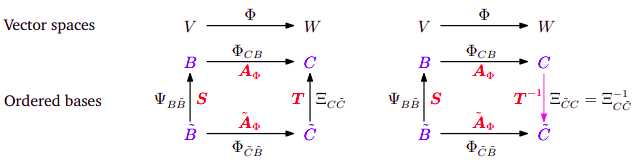
\includegraphics[
        width=\linewidth, 
        height=4cm,
        keepaspectratio,
    ]{images/maths-for-ml/basis-change.png}
    \caption*{
        For a homomorphism $\Phi  : V \to  W$ and ordered bases $B, \tilde{B}$ of $V$ and $C, \tilde{C}$ of $W$ (marked in \textcolor{blue}{blue}), we can express the mapping $\Phi _{\tilde{C} \tilde{B}}$ with respect to the bases $\tilde{B}, \tilde{C}$ equivalently as a composition of the homomorphisms $\Phi _{\tilde{C} \tilde{B}} = \Xi _{\tilde{C}C} \circ \Phi _{CB} \circ \Psi _{B\tilde{B}}$ with respect to the bases in the subscripts. 
        \\
        The corresponding transformation matrices are in \textcolor{red}{red}.
        \\
        We use $\Psi_{B\tilde{B}} = \text{id}_V$ and $\Xi _{C\tilde{C}} = \text{id}_W$ , i.e., the identity mappings that map vectors onto themselves, but with respect to a different basis.
        \hfill \cite{mfml/book/mml/Deisenroth-Faisal-Ong}
    }
\end{figure}


\begin{enumerate}
    \item \textbf{Theorem}: For a linear mapping $\Phi : V \to W$, ordered bases
    \hfill \cite{mfml/book/mml/Deisenroth-Faisal-Ong}
    \\
    .\hfill
    $
        B = (\bm{b}_1, \cdots , \bm{b}_n), \ 
        \tilde{B} = (\tilde{\bm{b}}_1, \cdots , \tilde{\bm{b}}_n)
    $
    \hfill \cite{mfml/book/mml/Deisenroth-Faisal-Ong}
    \\
    of $V$ and
    \hfill \cite{mfml/book/mml/Deisenroth-Faisal-Ong}
    \\
    .\hfill
    $
        C = (\bm{c}_1, \cdots , \bm{c}_n), \ 
        \tilde{C} = (\tilde{\bm{c}}_1, \cdots , \tilde{\bm{c}}_n)
    $
    \hfill \cite{mfml/book/mml/Deisenroth-Faisal-Ong}
    \\
    of $W$, and a transformation matrix $\bm{A}_\Phi$ of $\Phi$ with respect to $B$ and $C$, the corresponding transformation matrix $\tilde{\bm{A}} _\Phi$ with respect to the bases $\tilde{B}$ and $\tilde{C}$ is given as
    $
        \tilde{\bm{A}} \Phi = \bm{T}^{-1}\bm{A}_\Phi \bm{S}
    $.
    \hfill \cite{mfml/book/mml/Deisenroth-Faisal-Ong}
    \\
    Here, $\bm{S} \in \mathbb{R}^{n\times n}$ is the transformation matrix of $\text{id}_V$ that maps coordinates with respect to $\tilde{B}$ onto coordinates with respect to $B$, \ 
    and $\bm{T} \in \mathbb{R}^{m\times m}$ is the transformation matrix of $\text{id}_W$ that maps coordinates with respect to $\tilde{C}$ onto coordinates with respect to $C$.
    \hfill \cite{mfml/book/mml/Deisenroth-Faisal-Ong}

    \item \textbf{Proof}: we can write the vectors of the new basis $\tilde{B}$ of $V$ as a linear combination of the basis vectors of $B$, such that:
    \hfill \cite{mfml/book/mml/Deisenroth-Faisal-Ong}
    \\
    .\hfill
    $
        \tilde{\bm{b}}_j 
        = s_{1j} \bm{b}_1 + \cdots + s_{nj} \bm{b}_n 
        = \dsum^n _{i=1} s_{ij} \bm{b}_i 
        , j = 1, \cdots , n
    $
    \hfill \cite{mfml/book/mml/Deisenroth-Faisal-Ong}
    \\
    Similarly, we write the new basis vectors $\tilde{C}$ of $W$ as a linear combination of the basis vectors of $C$, which yields
    \hfill \cite{mfml/book/mml/Deisenroth-Faisal-Ong}
    \\
    .\hfill
    $
        \tilde{\bm{c}}_k 
        = t_{1k} \bm{c}_1 + \cdots + t_{mk} \bm{c}_m 
        = \dsum^m _{l=1} t_{lk} \bm{c}_l 
        , k = 1, \cdots , m
    $
    \hfill \cite{mfml/book/mml/Deisenroth-Faisal-Ong}
    \\
    We define $\bm{S} = ((s_{ij} )) \in \mathbb{R}^{n\times n}$ as the transformation matrix that maps coordinates with respect to $\tilde{B}$ onto coordinates with respect to $B$ and $\bm{T} = ((t_{lk})) \in R^{m\times m}$ as the transformation matrix that maps coordinates with respect to $\tilde{C}$ onto coordinates with respect to $C$. 
    In particular, the $j$-th column of $\bm{S}$ is the coordinate representation of $\tilde{\bm{b}}_j$ with respect to $B$ and the $k$-th column of $\bm{T}$ is the coordinate representation of $\tilde{\bm{c}}_k$ with respect to $C$. 
    Note that both $\bm{S}$ and $\bm{T}$ are regular.
    \hfill \cite{mfml/book/mml/Deisenroth-Faisal-Ong}
    \\
    We are going to look at $\Phi(\tilde{\bm{b}}_j )$ from two perspectives.
    \hfill \cite{mfml/book/mml/Deisenroth-Faisal-Ong}
    \begin{enumerate}
        \item Applying the mapping $\Phi$, we get that for all $j = 1, \cdots , n$
        \hfill \cite{mfml/book/mml/Deisenroth-Faisal-Ong}
        \\
        .\hfill
        $
            \Phi(\tilde{\bm{b}}_j )
            = \dsum^m_{k=1} \underset{\displaystyle \in W}{
                \underbrace{\tilde{a}_{kj} \textcolor{blue}{\tilde{\bm{c}}_k}}
            }
            = \dsum^m_{k=1} \tilde{a}_{kj} \textcolor{blue}{
                \dsum^m_{l=1} t_{lk} \bm{c}_l
            }
            = \dsum^m_{l=1} \dParenBrac{
                \textcolor{PineGreen}{\dsum^m_{k=1} t_{lk} \tilde{a}_{kj}} 
            }  \bm{c}_l
        $
        \hfill \cite{mfml/book/mml/Deisenroth-Faisal-Ong}
        \\
        where we first expressed the new basis vectors $\tilde{\bm{c}}_k \in W$ as linear combinations of the basis vectors $\bm{c}_l \in W$ and then swapped the order of summation.
        \hfill \cite{mfml/book/mml/Deisenroth-Faisal-Ong}


        \item when we express the $\tilde{\bm{b}}_j \in V$ as linear combinations of $\bm{b}_j \in V$ , we arrive at ($j = 1,\cdots, n$) :
        \hfill \cite{mfml/book/mml/Deisenroth-Faisal-Ong}
        \\
        .\hfill
        $
            \Phi (\tilde{\bm{b}}_j ) 
            = \Phi  \dParenBrac{ \textcolor{blue}{\dsum ^n _{i=1} s_{ij} \bm{b}_i}}
            = \dsum ^n _{i=1} s_{ij} \textcolor{red}{\Phi (\bm{b}_i)} 
            = \dsum^n _{i=1} s_{ij} \textcolor{red}{\dsum ^m _{l=1} a_{li} \bm{c}_l}
            = \dsum ^m _{l=1} \dParenBrac{ \textcolor{PineGreen}{\dsum^n _{i=1} s_{ij} a_{li}} } \bm{c}_l
        $
        \hfill \cite{mfml/book/mml/Deisenroth-Faisal-Ong}

        \item $
            \begin{aligned}
                \dsum^m_{k=1} t_{lk} \tilde{a}_{kj} = \dsum^n _{i=1} s_{ij} a_{li}
                \hspace{1cm}
                \Rightarrow 
                \bm{T} \tilde{\bm{A}}_\Phi = \bm{A}_\Phi \bm{S} 
                \in \mathbb{R}^{m\times n}
                \hspace{1cm}
                \Rightarrow 
                \tilde{\bm{A}}_\Phi = \bm{T}^{-1} \bm{A}_\Phi \bm{S}
            \end{aligned}
        $
        \hfill \cite{mfml/book/mml/Deisenroth-Faisal-Ong}        
    \end{enumerate}

    
\end{enumerate}






\subsection{Orthonormal Basis}


\begin{enumerate}
    \item 
\end{enumerate}




























\section{Linear Mappings}


\begin{figure}[H]
    \centering
    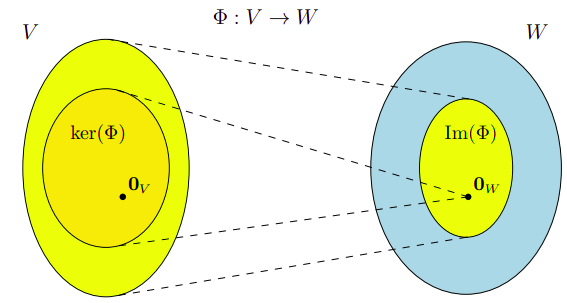
\includegraphics[
        width=\linewidth,
        height=4cm,
        keepaspectratio,
    ]{images/maths-for-ml/image-kernel-linear-mapping.png}
\end{figure}

\begin{enumerate}
    \item \textbf{Definition}: For vector spaces $V, W$, a mapping $\Phi : V \to W$ is called a linear mapping (or vector space homomorphism/ linear transformation) if
    \hfill \cite{mfml/book/mml/Deisenroth-Faisal-Ong}
    \\
    .\hfill
    $
        \forall \bm{x}, \bm{y} \in V \forall \lambda , \psi  \in \mathbb{R} : 
        \Phi(\lambda \bm{x} + \psi \bm{y}) = \lambda \Phi(\bm{x}) + \psi \Phi(\bm{y})
    $
    \hfill \cite{mfml/book/mml/Deisenroth-Faisal-Ong}

    \item we can represent linear mappings as matrices
    \hfill \cite{mfml/book/mml/Deisenroth-Faisal-Ong}

    \item For linear mappings $\Phi : V \to W$ and $\Psi : W \to X$, the mapping $\Psi \circ \Phi : V \to X$ is also linear.
    \hfill \cite{mfml/book/mml/Deisenroth-Faisal-Ong}

    \item If $\Phi : V \to W, \Psi : V \to W$ are linear, then $\Phi + \Psi$ and $\lambda\Phi, \lambda \in \mathbb{R}$, are linear, too.
    \hfill \cite{mfml/book/mml/Deisenroth-Faisal-Ong}
\end{enumerate}



\subsection{Matrix Representation of Linear Mappings}

\begin{enumerate}
    \item Any $n$-dimensional vector space is isomorphic to $\mathbb{R}^n$.
    \hfill \cite{mfml/book/mml/Deisenroth-Faisal-Ong}

    \item We consider a basis $\dCurlyBrac{\bm{b}_1, \cdots , \bm{b}_n}$ of an $n$-dimensional vector space $V$ .
    \hfill \cite{mfml/book/mml/Deisenroth-Faisal-Ong}
\end{enumerate}




\subsection{Image/Range \& Kernel/Null space}

\begin{enumerate}
    \item \textbf{Definition}: For $\Phi  : V \to W$, we define the image/range
    \hfill \cite{mfml/book/mml/Deisenroth-Faisal-Ong}
    \\
    .\hfill
    $
        \text{Im}(\Phi ) 
        := \Phi (V ) 
        = \dCurlyBrac{\bm{w} \in W|\exists \bm{v} \in V : \Phi (\bm{v}) = \bm{w}}
    $
    \hfill \cite{mfml/book/mml/Deisenroth-Faisal-Ong}

    \item \textbf{Definition}: For $\Phi  : V \to W$, we define the kernel/null space
    \hfill \cite{mfml/book/mml/Deisenroth-Faisal-Ong}
    \\
    .\hfill
    $
        \ker(\Phi ) 
        := \Phi ^{-1} (\bm{0}_W ) 
        = \dCurlyBrac{\bm{v} \in V : \Phi (\bm{v}) = \bm{0}_W }
    $
    \hfill \cite{mfml/book/mml/Deisenroth-Faisal-Ong}


    \item We also call $V$ and $W$ also the \textbf{domain} and \textbf{codomain} of $\Phi$, respectively.
    \hfill \cite{mfml/book/mml/Deisenroth-Faisal-Ong}

    \item The image is the set of vectors $\bm{w} \in W$ that can be “reached” by $\Phi$ from any vector in $V$ .
    \hfill \cite{mfml/book/mml/Deisenroth-Faisal-Ong}

    \item Intuitively, the kernel is the set of vectors $\bm{v} \in V$ that $\Phi$ maps onto the neutral element $\bm{0}_W \in W$.
    \hfill \cite{mfml/book/mml/Deisenroth-Faisal-Ong}

    \item It always holds that $\Phi(\bm{0}_V ) = \bm{0}_W$ and, therefore, $\bm{0}_V \in \ker(\Phi)$. 
    In particular, the null space is never empty.
    \hfill \cite{mfml/book/mml/Deisenroth-Faisal-Ong}

    \item $Im(\Phi) \subseteq W$ is a subspace of $W$, and $\ker(\Phi) \subseteq V$ is a subspace of $V$ .
    \hfill \cite{mfml/book/mml/Deisenroth-Faisal-Ong}

    \item $\Phi$ is injective (one-to-one) if and only if $\ker(\Phi) = \dCurlyBrac{\bm{0}}$.
    \hfill \cite{mfml/book/mml/Deisenroth-Faisal-Ong}

    \item \textbf{Rank-Nullity Theorem}: For vector spaces $V, W$ and a linear mapping $\Phi : V \to W$ it holds that $\dim(\ker(\Phi)) + \dim(\text{Im}(\Phi)) = \dim(V )$.
    \hfill \cite{mfml/book/mml/Deisenroth-Faisal-Ong}
    \begin{enumerate}
        \item The rank-nullity theorem is also referred to as the \textbf{fundamental theorem of linear mappings}
        \hfill \cite{mfml/book/mml/Deisenroth-Faisal-Ong}

        \item If $\dim(\text{Im}(\Phi )) < \dim(V )$, then $\ker(\Phi)$ is non-trivial, i.e., the kernel contains more than $\bm{0}_V$ and $\dim(\ker(\Phi)) \geq 1$.
        \hfill \cite{mfml/book/mml/Deisenroth-Faisal-Ong}

        \item If $\bm{A}_\Phi $ is the transformation matrix of $\Phi$  with respect to an ordered basis and $\dim(\text{Im}(\Phi )) < \dim(V )$, then the system of linear equations $\bm{A}_\Phi \bm{x} = \bm{0}$ has infinitely many solutions.
        \hfill \cite{mfml/book/mml/Deisenroth-Faisal-Ong}

        \item If $\dim(V ) = \dim(W)$, then the following three-way equivalence holds:
        \begin{enumerate}
            \item $\Phi$ is injective
            \item $\Phi$ is surjective
            \item $\Phi$ is bijective
        \end{enumerate}
        since $\text{Im}(\Phi) \subseteq W$.
    \end{enumerate}
\end{enumerate}













\section{Affine Mapping}

\begin{enumerate}
    \item \textbf{Definition}: For two vector spaces $V, W$, a linear mapping $\Phi : V \to W$, and $\bm{a} \in W$, the mapping:
    \hfill \cite{mfml/book/mml/Deisenroth-Faisal-Ong}
    \\
    .\hfill
    $ \phi : V \to W $ such that $ \bm{x} \mapsto \bm{a} + \Phi(\bm{x}) $
    \hfill \cite{mfml/book/mml/Deisenroth-Faisal-Ong}
    \\
    is an affine mapping from $V$ to $W$. 
    The vector a is called the \textbf{translation vector} of $\phi$.
    \hfill \cite{mfml/book/mml/Deisenroth-Faisal-Ong}

    \item Every affine mapping $\phi  : V \to W$ is also the composition of a linear mapping $\phi  : V \to W$ and a translation $\tau : W \to W$ in $W$, such that $\phi  = \tau \circ \phi $. 
    The mappings $\phi $ and $\tau$ are uniquely determined.
    \hfill \cite{mfml/book/mml/Deisenroth-Faisal-Ong}

    \item The composition $\phi ^\prime \circ \phi $ of affine mappings $\phi  : V \to W, \phi ^\prime: W \to X$ is affine.
    \hfill \cite{mfml/book/mml/Deisenroth-Faisal-Ong}

    \item Affine mappings keep the geometric structure invariant. 
    They also preserve the dimension and parallelism.
    \hfill \cite{mfml/book/mml/Deisenroth-Faisal-Ong}
\end{enumerate}



























\section{Injective, Surjective, Bijective Mappings}

\textbf{Definition}: Consider a mapping $\Phi : \mathcal{V} \to \mathcal{W}$, where $\mathcal{V}, \mathcal{W}$ can be arbitrary sets. 
Then $\Phi$ is called:
\hfill \cite{mfml/book/mml/Deisenroth-Faisal-Ong}

\begin{enumerate}
    \item \textbf{Injective} if $\forall \bm{x}, \bm{y} \in \mathcal{V} : \Phi(\bm{x}) = \Phi(\bm{y}) \Rightarrow \bm{x} = \bm{y}$
    \hfill \cite{mfml/book/mml/Deisenroth-Faisal-Ong}

    \item \textbf{Surjective} if $\Phi(\mathcal{V}) = \mathcal{W}$
    \hfill \cite{mfml/book/mml/Deisenroth-Faisal-Ong}
    \begin{enumerate}
        \item If $\Phi$ is surjective, then every element in $\mathcal{W}$ can be “reached” from $\mathcal{V}$ using $\Phi$.
        \hfill \cite{mfml/book/mml/Deisenroth-Faisal-Ong}
    \end{enumerate}
    
    \item \textbf{Bijective} if it is injective and surjective
    \hfill \cite{mfml/book/mml/Deisenroth-Faisal-Ong}
    \begin{enumerate}
        \item A bijective $\Phi$ can be “undone”, i.e., there exists a mapping $\Psi : W \to V$ so that $\Psi \circ \Phi(\bm{x}) = \bm{x}$.
        \hfill \cite{mfml/book/mml/Deisenroth-Faisal-Ong}

        \item This mapping $\Psi$ is then called the inverse of $\Phi$ and normally denoted by $\Phi^{-1}$.
        \hfill \cite{mfml/book/mml/Deisenroth-Faisal-Ong}
    \end{enumerate}    

\end{enumerate}


















\section{Special cases of Linear mappings}

\textbf{Definition}: Consider a mapping $\Phi : V \to W$, where $V, W$ can be arbitrary vector spaces. 
Then:
\hfill \cite{mfml/book/mml/Deisenroth-Faisal-Ong}

\begin{enumerate}
    \item \textbf{Isomorphism}: $\Phi : V \to W$ linear and bijective
    \hfill \cite{mfml/book/mml/Deisenroth-Faisal-Ong}
    \begin{enumerate}
        \item \textbf{Theorem}: Finite-dimensional vector spaces $V$ and $W$ are isomorphic if and only if $\dim(V ) = \dim(W)$.
        \hfill \cite{mfml/book/mml/Deisenroth-Faisal-Ong}

        \item there exists a linear, bijective mapping between two vector spaces of the same dimension.
        Intuitively, this means that vector spaces of the same dimension are kind of the same thing, as they can be transformed into each other without incurring any loss.
        \hfill \cite{mfml/book/mml/Deisenroth-Faisal-Ong}

        \item It gives the justification to treat $\mathbb{R}^{m\times n}$ (the vector space of $m \times n$-matrices) and $\mathbb{R}^{mn}$ (the vector space of vectors of length $mn$) the same, as their dimensions are $mn$, and there exists a linear, bijective mapping that transforms one into the other.
        \hfill \cite{mfml/book/mml/Deisenroth-Faisal-Ong}

        \item If $\Phi : V \to W$ is an isomorphism, then $\Phi ^{-1} : W \to V$ is an isomorphism, too.
        \hfill \cite{mfml/book/mml/Deisenroth-Faisal-Ong}
    \end{enumerate}

    \item \textbf{Endomorphism}: $\Phi : V \to V$ linear
    \hfill \cite{mfml/book/mml/Deisenroth-Faisal-Ong}

    \item \textbf{Automorphism}: $\Phi : V \to V$ linear and bijective
    \hfill \cite{mfml/book/mml/Deisenroth-Faisal-Ong}

    \item \textbf{identity mapping} or \textbf{identity automorphism}: $id_V : V \to V , \bm{x} \mapsto \bm{x}$
    \hfill \cite{mfml/book/mml/Deisenroth-Faisal-Ong}
\end{enumerate}



















\section{Transformation Matrix ( $A_\Phi$ )}

\begin{enumerate}
    \item \textbf{Definition}: Consider vector spaces $V$, $W$ with corresponding (ordered) bases $B = (\bm{b}_1, \cdots , \bm{b}_n)$ and $C = (\bm{c}_1, \cdots , \bm{c}_m)$. 
    Moreover, we consider a linear mapping $\Phi : V \to W$. 
    For $j \in \dCurlyBrac{1, \cdots , n}$,
    \hfill \cite{mfml/book/mml/Deisenroth-Faisal-Ong}
    \\
    .\hfill
    $
        \Phi(\bm{b}_j ) = \alpha _{1j} \bm{c}_1 + \cdots + \alpha _{mj} \bm{c}_m 
        = \dsum^m_{i=1} \alpha _{ij} \bm{c}_i
    $
    \hfill \cite{mfml/book/mml/Deisenroth-Faisal-Ong}
    \\
    is the unique representation of $\Phi(\bm{b}_j )$ with respect to $C$. 
    Then, we call the $m \times n$-matrix $\bm{A}_\Phi$, whose elements are given by $\bm{A}_\Phi(i, j) = \alpha_{ij}$ the transformation matrix of $\Phi$ (with respect to the ordered bases $B$ of $V$ and $C$ of $W$  ).
    \hfill \cite{mfml/book/mml/Deisenroth-Faisal-Ong}

    \item The transformation matrix can be used to map coordinates with respect to an ordered basis in $V$ to coordinates with respect to an ordered basis in $W$.
    \hfill \cite{mfml/book/mml/Deisenroth-Faisal-Ong}

    \item Consider vector spaces $V, W, X$. 
    We already know that for linear mappings $\Phi  : V \to  W$ and $\Psi : W \to  X$ the mapping $\Psi \circ \Phi  : V \to  X$ is also linear. 
    With transformation matrices $\bm{A}_\Phi$  and $\bm{A}_\Psi$ of the corresponding mappings, the overall transformation matrix is $\bm{A}_{\Psi\circ\Phi}  = \bm{A}_\Psi \bm{A}_\Phi$ .
    \hfill \cite{mfml/book/mml/Deisenroth-Faisal-Ong}

    \item 
    $\bm{A}_\Phi$  is the transformation matrix of a linear mapping $\Phi _{CB} : V \to  W$ with respect to the bases $B, C$.
    \hfill \cite{mfml/book/mml/Deisenroth-Faisal-Ong}
    \\[0.2cm]
    $\tilde{\bm{A}}_\Phi$  is the transformation matrix of the linear mapping $\Phi_ {\tilde{C}\tilde{B}} : V \to  W$ with respect to the bases $\tilde{B}, \tilde{C}$.
    \hfill \cite{mfml/book/mml/Deisenroth-Faisal-Ong}
    \\[0.2cm]
    $\bm{S}$ is the transformation matrix of a linear mapping $\Psi _{B\tilde{B}} : V \to  V$ (automorphism) that represents $\tilde{B}$ in terms of $B$. Normally, $\Psi  = \text{id}_V$ is the identity mapping in $V$ .
    \hfill \cite{mfml/book/mml/Deisenroth-Faisal-Ong}
    \\[0.2cm]
    $\bm{T}$ is the transformation matrix of a linear mapping $\Xi _{C\tilde{C}} : W \to  W$ (automorphism) that represents $\tilde{C}$ in terms of $C$. Normally, $\Xi  = \text{id}_W$ is the identity mapping in $W$.
    \hfill \cite{mfml/book/mml/Deisenroth-Faisal-Ong}
    \\[0.2cm]
    If we (informally) write down the transformations just in terms of bases, then $\bm{A}_\Phi  : B \to  C$, $\tilde{\bm{A}}_\Phi  : \tilde{B} \to  \tilde{C}$, $\bm{S} : \tilde{B} \to  B$, $\bm{T} : \tilde{C} \to  C$ and $\bm{T}^{-1} : C \to  \bm{C}$, and
    \hfill \cite{mfml/book/mml/Deisenroth-Faisal-Ong}
    \\[0.2cm]
    .\hfill
    $
        \tilde{B} \to  \tilde{C} = \textcolor{blue}{\tilde{B} \to  B} \textcolor{red}{\to  C} \to  \tilde{C} 
        \Rightarrow
        \tilde{\bm{A}}_\Phi  = \bm{T}^{-1} \textcolor{red}{\bm{A}_\Phi} \textcolor{blue}{\bm{S}}
    $
    \hfill \cite{mfml/book/mml/Deisenroth-Faisal-Ong}
    \\[0.2cm]
    Note that the execution order is from \textbf{right to left} because vectors are multiplied at the right-hand side so that 
    \hfill \cite{mfml/book/mml/Deisenroth-Faisal-Ong}
    \\[0.2cm]
    .\hfill
    $\bm{x} \mapsto  \bm{Sx} \mapsto  \bm{A}_\Phi (\bm{Sx}) \mapsto \bm{T}^{-1}(\bm{A}_\Phi (\bm{Sx})) = \tilde{\bm{A}}_\Phi \bm{x}$.
    \hfill \cite{mfml/book/mml/Deisenroth-Faisal-Ong}

    \item  Orthogonal matrices define transformations that are rotations (with the possibility of flips).
    \hfill \cite{mfml/book/mml/Deisenroth-Faisal-Ong}
\end{enumerate}






\section{Coordinates}

\begin{enumerate}
    \item Consider a vector space $V$ and an ordered basis $B = (\bm{b}_1, \cdots , \bm{b}_n)$ of $V$ . 
    For any $\bm{x} \in V$ we obtain a unique representation (linear combination):
    \hfill \cite{mfml/book/mml/Deisenroth-Faisal-Ong}
    \\
    .\hfill
    $
        \bm{x} = \alpha_1 \bm{b}_1 + \cdots + \alpha_n \bm{b}_n
    $
    \hfill \cite{mfml/book/mml/Deisenroth-Faisal-Ong}
    \\
    of $\bm{x}$ with respect to $B$. 
    Then $\alpha_1, \cdots , \alpha_n$ are the coordinates of $\bm{x}$ with respect to $B$, and the vector:
    \hfill \cite{mfml/book/mml/Deisenroth-Faisal-Ong}
    \\
    .\hfill
    $
        \bm{\alpha} = \begin{bmatrix}
            \alpha_1 \\
            \vdots \\
            \alpha_n
        \end{bmatrix}
        \in \mathbb{R}^n
    $
    \hfill \cite{mfml/book/mml/Deisenroth-Faisal-Ong}
    \\
    is the \textbf{coordinate vector/ coordinate} representation of $\bm{x}$ with respect to the ordered basis $B$.
    \hfill \cite{mfml/book/mml/Deisenroth-Faisal-Ong}

    \item A basis effectively defines a coordinate system.
    \hfill \cite{mfml/book/mml/Deisenroth-Faisal-Ong}

    \item For an $n$-dimensional vector space $V$ and an ordered basis $B$ of $V$ , the mapping $\Phi : \mathbb{R}^n \to V , \Phi(\bm{e}_i) = \bm{b}_i , i = 1, \cdots , n$, is linear, where $(\bm{e}_1, \cdots , \bm{e}_n)$ is the standard basis of $\mathbb{R}^n$.
    \hfill \cite{mfml/book/mml/Deisenroth-Faisal-Ong}

    \item The coordinates of $\Phi(\bm{b}_j )$ with respect to the ordered basis $C$ of $W$ are the $j$-th column of $\bm{A}_\Phi$.
    \hfill \cite{mfml/book/mml/Deisenroth-Faisal-Ong}
    \hfill \cite{mfml/book/mml/Deisenroth-Faisal-Ong}
    \begin{enumerate}
        \item Consider (finite-dimensional) vector spaces $V$, $W$ with ordered bases $B$, $C$ and a linear mapping $\Phi : V \to W$ with transformation matrix $\bm{A}_\Phi$.
        \hfill \cite{mfml/book/mml/Deisenroth-Faisal-Ong}

        \item If $\hat{\bm{x}}$ is the coordinate vector of $\bm{x} \in V$ with respect to $B$ and $\hat{\bm{y}}$ the coordinate vector of $\bm{y} = \Phi(\bm{x}) \in W$ with respect to $C$, then $\hat{\bm{y}} = \bm{A}_\Phi \hat{\bm{x}}$.
        \hfill \cite{mfml/book/mml/Deisenroth-Faisal-Ong}
    \end{enumerate}    
\end{enumerate}




























\chapter{Systems of Linear Equations}

% \begin{enumerate}
%     \item \textbf{Algebra} is constructing a set of objects (symbols) and a set of rules to manipulate these objects.
%     \hfill \cite{mfml/book/mml/Deisenroth-Faisal-Ong}

%     \item \textbf{Linear algebra} is the study of vectors and certain rules to manipulate vectors.
%     \hfill \cite{mfml/book/mml/Deisenroth-Faisal-Ong}
% \end{enumerate}


\begin{customArrayStretch}{1.3}
\begin{table}[H]
    \centering
    \begin{tabular}{| l | l  l |}
        \hline

        coefficients & $a_{ij}$    & $\in \mbbR$ \\ \hline

        constants & $b_{i}$     & $\in \mbbR$ \\ \hline

        unknowns & $x_{i}$     & $\in \mbbR$ \\ \hline

    \end{tabular}
    \caption*{Notations}
\end{table}
\end{customArrayStretch}


\vspace{0.5cm}


\begin{enumerate}
    \item \textbf{general form} of a system of linear equations:
    \\
    .\hfill
    $
        \begin{aligned}
            a_{11}x_1\  & +\ & \cdots\ & +\ & a_{1n}x_n\ & =\ & b_1 \\
            & & & \vdots \\
            a_{m1}x_1\  & +\ & \cdots\ & +\ & a_{mn}x_n\ & =\ & b_m
        \end{aligned}
    $
    \hfill \cite{mfml/book/mml/Deisenroth-Faisal-Ong}
    \vspace{0.2cm}
    \begin{enumerate}
        \item $x_1, \cdots , x_n$ are the \textbf{unknowns} of this system.

        \item Every $n$-tuple $(x_1, \cdots , x_n) \in \mbbR^n$ that satisfies this system is a \textbf{solution} of the linear equation system.
    \end{enumerate}


    \item \textbf{compact notation}:
    \\[0.2cm]
    $
        \begin{bmatrix}a_{11}\\ \vdots\\ a_{m1}\end{bmatrix} \bm{x}_1 +
        \begin{bmatrix}a_{12}\\ \vdots\\ a_{m2}\end{bmatrix} \bm{x}_2 +
        \cdots +
        \begin{bmatrix}a_{1n}\\ \vdots\\ a_{mn}\end{bmatrix} \bm{x}_n =
        \begin{bmatrix}b_{1}\\ \vdots\\ b_{m}\end{bmatrix}
    \Longleftrightarrow
        \underset{\displaystyle\bm{A}}{\underbrace{\begin{bmatrix}
            a_{11} & \cdots & a_{1n} \\
            \vdots & \ddots & \vdots \\
            a_{m1} & \cdots & a_{mn}
        \end{bmatrix}}} \
        \underset{\displaystyle\bm{x}}{\underbrace{\begin{bmatrix} x_{1} \\ \vdots \\ x_{n} \end{bmatrix}}}
        =
        \underset{\displaystyle\bm{b}}{\underbrace{\begin{bmatrix} b_{1} \\ \vdots \\ b_{m} \end{bmatrix}}}
    $
    \hfill \cite{mfml/book/mml/Deisenroth-Faisal-Ong}



\end{enumerate}


\vspace{0.5cm}
\textbf{Note}:
\begin{enumerate}
    \item In general, for a real-valued system of linear equations we obtain either no, exactly one, or infinitely many solutions.
    \hfill \cite{mfml/book/mml/Deisenroth-Faisal-Ong}

    \item \textbf{Geometric Interpretation of Systems of Linear Equations}:
    In a system of linear equations with two variables $x_1$, $x_2$, each linear equation defines a line on the $x_1x_2$-plane. Since a solution to a system of linear equations must satisfy all equations simultaneously, the solution set is the intersection of these lines. This intersection set can be a line (if the linear equations describe the same line), a point, or empty (when the lines are parallel).
    \hfill \cite{mfml/book/mml/Deisenroth-Faisal-Ong}
    \\
    Similarly, for three variables, each linear equation determines a plane in three-dimensional space. When we intersect these planes, i.e., satisfy all linear equations at the same time, we can obtain a solution set that is a plane, a line, a point or empty (when the planes have no common intersection).
    \hfill \cite{mfml/book/mml/Deisenroth-Faisal-Ong}

    \item the product $Ax$ is a (linear) combination of the columns of $A$
    \hfill \cite{mfml/book/mml/Deisenroth-Faisal-Ong}

    \item \textbf{Augmented Matrix} ( $\dSquareBrac{\bm{A}|\bm{b}}$ ):
    \\[0.2cm]
    $
        \left[
        \begin{array}{ccc|c}
            a_{11} & \cdots & a_{1n} & b_{1}\\
            \vdots & \ddots & \vdots & \vdots \\
            a_{m1} & \cdots & a_{mn} & b_{m}
        \end{array}
        \right]
    $

    \item The solution set of a homogeneous system of linear equations $\bm{Ax} = \bm{0}$ with $n$ unknowns $\bm{x} = [x_1, \cdots , x_n]^\top$ is a subspace of $\mbbR^n$.
    \hfill \cite{mfml/book/mml/Deisenroth-Faisal-Ong}

    \item Every subspace $U \subseteq (\mbbR^n , +, \cdot)$ is the solution space of a homogeneous system of linear equations $\bm{Ax} = \bm{0}$ for $\bm{x} \in \mbbR^n$.
    \hfill \cite{mfml/book/mml/Deisenroth-Faisal-Ong}

    \item The solution of an inhomogeneous system of linear equations $\bm{Ax} = \bm{b}, \bm{b} \neq \bm{0}$ is not a subspace of $\mbbR^n$.
    \hfill \cite{mfml/book/mml/Deisenroth-Faisal-Ong}


\end{enumerate}








\section{Types of Solutions}

\begin{enumerate}

\item \textbf{Unique Solution}:
\begin{enumerate}
    \item The system has exactly one solution.
    \hfill \cite{common/online/chatgpt}

    \item \textbf{Graphically}: The lines (or planes) intersect at a single point.
    \hfill \cite{common/online/chatgpt}

    \item \textbf{Algebraically}: The equations are independent and consistent.
    \hfill \cite{common/online/chatgpt}
\end{enumerate}

\item \textbf{Infinite Solutions}:
\begin{enumerate}
    \item The system has infinitely many solutions.
    \hfill \cite{common/online/chatgpt}

    \item \textbf{Graphically}: The lines (or planes) are exactly the same (i.e., they overlap).
    \hfill \cite{common/online/chatgpt}

    \item \textbf{Algebraically}: The equations are dependent and consistent.
    \hfill \cite{common/online/chatgpt}
\end{enumerate}

\item \textbf{No Solution}:
\begin{enumerate}
    \item The system has no common solution.
    \hfill \cite{common/online/chatgpt}

    \item \textbf{Graphically}: The lines are parallel (in 2D) and never meet.
    \hfill \cite{common/online/chatgpt}

    \item \textbf{Algebraically}: The system is inconsistent.
    \hfill \cite{common/online/chatgpt}
\end{enumerate}

\end{enumerate}


\section{Finding Solutions using Matrix Inverse}

\begin{enumerate}
    \item if $\bm{A}$ is a square matrix and invertible (strict conditions): $\bm{x} = \bm{A}^{-1}\bm{b}$
    \hfill \cite{mfml/book/mml/Deisenroth-Faisal-Ong}

    \item if $\bm{A}$ has linearly independent columns (mild assumptions): $\bm{x} = (\bm{A}^\top  \bm{A})^{-1}\bm{A}^\top \bm{b}$
    \hfill \cite{mfml/book/mml/Deisenroth-Faisal-Ong}

    \item for reasons of numerical precision it is generally not recommended to compute the inverse or pseudo-inverse
    \hfill \cite{mfml/book/mml/Deisenroth-Faisal-Ong}
\end{enumerate}


\section{Finding Solutions using Elementary Transformations}

\begin{enumerate}
    \item keep the solution set the same, but that transform the equation system into a simpler form
    \hfill \cite{mfml/book/mml/Deisenroth-Faisal-Ong}

    \item Operations:
    \begin{enumerate}
        \item Exchange of two equations (rows in the matrix representing the system of equations)
        \hfill \cite{mfml/book/mml/Deisenroth-Faisal-Ong}

        \item Multiplication of an equation (row) with a constant $\lambda \in \mbbR \backslash \dCurlyBrac{0}$
        \hfill \cite{mfml/book/mml/Deisenroth-Faisal-Ong}

        \item Addition of two equations (rows)
        \hfill \cite{mfml/book/mml/Deisenroth-Faisal-Ong}
    \end{enumerate}

    \item Disadvantages:
    \begin{enumerate}
        \item for systems with millions of variables, it is impractical as the required number of arithmetic operations scales cubically in the number of simultaneous equations.
        \hfill \cite{mfml/book/mml/Deisenroth-Faisal-Ong}
    \end{enumerate}
\end{enumerate}



\subsection{Row-Echelon Form (REF)}

\begin{enumerate}
    \item
    \begin{definition}[REF: pivot]
        The leading coefficient of a row (first nonzero number from the left) is called the pivot and is always strictly to the right of the pivot of the row above it.
        \hfill \cite{mfml/book/mml/Deisenroth-Faisal-Ong}
    \end{definition}

    \item any equation system in row-echelon form always has a “staircase” structure
    \hfill \cite{mfml/book/mml/Deisenroth-Faisal-Ong}

    \item A matrix is in row-echelon form if
    \begin{enumerate}
        \item All rows that contain only zeros are at the bottom of the matrix; correspondingly, all rows that contain at least one nonzero element are on top of rows that contain only zeros.
        \hfill \cite{mfml/book/mml/Deisenroth-Faisal-Ong}

        \item Looking at nonzero rows only, the first nonzero number from the left (also called the \textbf{pivot} or the \textbf{leading coefficient}) is always strictly to the right of the pivot of the row above it.
        \hfill \cite{mfml/book/mml/Deisenroth-Faisal-Ong}
    \end{enumerate}

    \item The variables corresponding to the pivots in the row-echelon form are called basic variables and the other variables are free variables.
    \hfill \cite{mfml/book/mml/Deisenroth-Faisal-Ong}

    \item we express the right-hand side of the equation system using the pivot columns, such that $\bm{b} = \dsum^P_{i=1} \lambda_i\ \bm{p}_i$, where $\bm{p}_i$ , $i = 1, \cdots , P$, are the pivot columns.
    \\
    The $\lambda_i$ are determined easiest if we start with the rightmost pivot column and work our way to the left.
    \hfill \cite{mfml/book/mml/Deisenroth-Faisal-Ong}


\end{enumerate}



\subsection{Reduced Row-Echelon Form (RREF)/ row-reduced echelon form/ row canonical form \cite{mfml/book/mml/Deisenroth-Faisal-Ong}}

\begin{enumerate}
    \item An equation system is in reduced reduced row-echelon form if:
    \begin{enumerate}
        \item It is in row-echelon form.
        \hfill \cite{mfml/book/mml/Deisenroth-Faisal-Ong}

        \item Every pivot is $1$.
        \hfill \cite{mfml/book/mml/Deisenroth-Faisal-Ong}

        \item The pivot is the only non-zero entry in its column.
        \hfill \cite{mfml/book/mml/Deisenroth-Faisal-Ong}
    \end{enumerate}

    \item Gaussian elimination is an algorithm that performs elementary transformations to bring a system of linear equations into reduced row-echelon form.
    \hfill \cite{mfml/book/mml/Deisenroth-Faisal-Ong}
\end{enumerate}



\subsection{Particular Solution/ Special solution}

\begin{customArrayStretch}{1.3}
\begin{table}[H]
    \centering
    \begin{tabular}{|l|l|l|}
        \hline
        \textbf{Term} &
            \textbf{Scope} &
            \textbf{Context} \\ \hline \hline

        \textbf{Unique Solution} &
            One and only one solution &
            Systems of equations \\ \hline

        \textbf{Particular Solution} &
            One of possibly many solutions &
            Differential equations, infinite solution systems \\ \hline

    \end{tabular}
    \caption*{Unique Solution VS Particular Solution \cite{common/online/chatgpt}}
\end{table}
\end{customArrayStretch}


\begin{enumerate}
    \item this is not the only solution of this system of linear equations.
    \hfill \cite{mfml/book/mml/Deisenroth-Faisal-Ong}

    \item To capture all the other solutions, we need to be creative in generating $0$ in a non-trivial way using the columns of the matrix: Adding $0$ to our special solution \textbf{does not} change the special solution.
    \hfill \cite{mfml/book/mml/Deisenroth-Faisal-Ong}


\end{enumerate}




\subsection{Finding Solutions to $Ax=0$: Minus-$1$ Trick \cite{mfml/book/mml/Deisenroth-Faisal-Ong}}

Let $\bm{A}$ is in reduced row-echelon form without any rows that just contain zeros:\\
.\hfill
$
    \bm{A}
    =
    \begin{bmatrix}
        0 & \cdots & 0 & \mathbf{1} & * & \cdots & * & 0 & * & \cdots & * & 0 & * & \cdots & * \\
        \vdots & & \vdots & 0 & 0 & \cdots & 0 & \mathbf{1} & * & \cdots & * & \vdots & \vdots & & \vdots\\
        \vdots & & \vdots & \vdots & \vdots &  & \vdots & 0 & \vdots & & \vdots & \vdots & \vdots & & \vdots\\
        \vdots & & \vdots & \vdots & \vdots &  & \vdots & \vdots & \vdots & & \vdots & 0 & \vdots & & \vdots\\
        0 & \cdots & 0 & 0 & 0 & \cdots & 0 & 0 & 0 & \cdots & 0 & \mathbf{1} & * & \cdots & *
    \end{bmatrix}
    \in \mbbR^{k\times n}
$
\hfill \cite{mfml/book/mml/Deisenroth-Faisal-Ong}

\vspace{0.2cm}

\begin{enumerate}
    \item $*$ can be an arbitrary real number
    \hfill \cite{mfml/book/mml/Deisenroth-Faisal-Ong}

    \item constraints:
    \begin{enumerate}
        \item first nonzero entry per row must be $1$
        \hfill \cite{mfml/book/mml/Deisenroth-Faisal-Ong}

        \item all other entries in the corresponding column must be $0$
        \hfill \cite{mfml/book/mml/Deisenroth-Faisal-Ong}
    \end{enumerate}

    \item The columns $j_1, \cdots , j_k$ with the pivots (marked in \textbf{bold}) are the standard unit vectors $e_1, \cdots , e_k \in \mbbR^k$.
    \hfill \cite{mfml/book/mml/Deisenroth-Faisal-Ong}

    \item We extend this matrix to an $n \times n$-matrix $\tilde{\bm{A}}$ by adding $n - k$ rows of the form
    $
        \begin{bmatrix}
            0 & \cdots & 0 & -1 & 0 & \cdots & 0
        \end{bmatrix}
    $
    so that the diagonal of the augmented matrix $\tilde{\bm{A}}$ contains either $1$ or $-1$.
    \hfill \cite{mfml/book/mml/Deisenroth-Faisal-Ong}

    \item columns of $\tilde{\bm{A}}$ that contain the $-1$ as pivots are solutions of the homogeneous equation system $Ax = 0$.
    \hfill \cite{mfml/book/mml/Deisenroth-Faisal-Ong}

    \item To be more precise, these columns form a basis of the solution space of $\bm{Ax} = \bm{0}$, called the kernel or null space.
    \hfill \cite{mfml/book/mml/Deisenroth-Faisal-Ong}
\end{enumerate}





\subsection{General Solution (= Particular Solution + Solutions to $Ax=0$)}

\begin{customArrayStretch}{1.3}
\begin{table}[H]
    \centering
    \begin{tabular}{|l|l|l|}
        \hline
        \textbf{Term} &
            \textbf{What it tells you} &
            \textbf{Context} \\ \hline

        \textbf{Infinite Solutions} &
            The quantity of solutions &
            Systems of equations \\ \hline

        \textbf{General Solution} &
            A formula for all solutions &
            Differential equations, algebra \\ \hline

    \end{tabular}
    \caption*{Infinite Solutions VS General Solution \cite{common/online/chatgpt}}
\end{table}
\end{customArrayStretch}


\begin{enumerate}
    \item The general approach we followed consisted of the following three steps:
    \begin{enumerate}
        \item Find a particular solution to $\bm{Ax} = \bm{b}$
        \hfill \cite{mfml/book/mml/Deisenroth-Faisal-Ong}

        \item Find all solutions to $\bm{Ax} = \bm{0}$
        \hfill \cite{mfml/book/mml/Deisenroth-Faisal-Ong}

        \item Combine the solutions from steps 1. and 2. to the general solution.
        \hfill \cite{mfml/book/mml/Deisenroth-Faisal-Ong}
    \end{enumerate}


\end{enumerate}









\section{Approximate Solution}

\begin{enumerate}
    \item Projections allow us to look at situations where we have a linear system $\bm{Ax} = \bm{b}$ without a solution.
    This means that b does not lie in the span of $\bm{A}$, i.e., the vector $\bm{b}$ does not lie in the subspace spanned by the columns of $\bm{A}$.
    \hfill \cite{mfml/book/mml/Deisenroth-Faisal-Ong}

    \item The idea is to find the vector in the subspace spanned by the columns of $\bm{A}$ that is closest to $\bm{b}$, i.e., we compute the orthogonal projection of $\bm{b}$ onto the subspace spanned by the columns of $\bm{A}$.
    This problem arises often in practice, and the solution is called the \textbf{least-squares solution} (assuming the dot product as the inner product) of an overdetermined system.
    \hfill \cite{mfml/book/mml/Deisenroth-Faisal-Ong}
\end{enumerate}











\section{Finding Solutions using stationary iterative methods - TODO}

\begin{enumerate}
    \item Let $\bm{x}_\ast$ be a solution of $\bm{Ax} = \bm{b}$.
    \hfill \cite{mfml/book/mml/Deisenroth-Faisal-Ong}

    \item The key idea of these iterative methods is to set up an iteration of the form
    $
        \bm{x}^{(k+1)} = C\bm{x}^{(k)} + d
    $
    for suitable $C$ and $d$ that reduces the residual error $\dnorm{\bm{x}^{(k+1)} - \bm{x}_\ast}$ in every iteration and converges to $\bm{x}_\ast$.
    \hfill \cite{mfml/book/mml/Deisenroth-Faisal-Ong}

\end{enumerate}


\subsection{Richardson method - TODO}


\subsection{Jacobi method - TODO}


\subsection{Gauß-Seidel method - TODO}


\subsection{successive over-relaxation method - TODO}


\section{Finding Solutions using Krylov subspace methods - TODO}


\subsection{conjugate gradients - TODO}


\subsection{generalized minimal residual - TODO}


\subsection{biconjugate gradients - TODO}





































\partition{Artificial Intelligence (AI)}
\chapter{AI: Introduction}\label{Artificial Intelligence: Introduction}

\begin{enumerate}
    \item The field of artificial intelligence, or AI, attempts not just to \textbf{understand} but also to \textbf{build} intelligent entities.
    \hfill \cite{ai/book/Artificial-Intelligence-A-Modern-Approach/Russell-Norvig}

    \item AI currently encompasses a huge variety of subfields, ranging from the general (learning and perception) to the specific, such as playing chess, proving mathematical theorems, writing poetry, driving a car on a crowded street, and diagnosing diseases.
    \hfill \cite{ai/book/Artificial-Intelligence-A-Modern-Approach/Russell-Norvig}

    \item AI is relevant to any intellectual task; it is truly a universal field.
    \hfill \cite{ai/book/Artificial-Intelligence-A-Modern-Approach/Russell-Norvig}

    \item A system is \textbf{rational} if it does the “right thing,” given what it knows.
    \hfill \cite{ai/book/Artificial-Intelligence-A-Modern-Approach/Russell-Norvig}
\end{enumerate}






\section{Approaches to AI}\label{Artificial Intelligence: Introduction/Approaches to AI}

\subsection{Acting humanly: The Turing Test approach}\label{Artificial Intelligence: Introduction/Approaches to AI/Acting humanly: The Turing Test approach}


\begin{enumerate}
    \item The \textbf{Turing Test}\label{Artificial Intelligence: Introduction/Approaches to AI/Acting humanly: The Turing Test approach/Turing Test}, proposed by \textbf{Alan Turing} (1950), was designed to provide a satisfactory operational definition of intelligence.
    \hfill \cite{ai/book/Artificial-Intelligence-A-Modern-Approach/Russell-Norvig}

    \item A computer passes the test if a human interrogator, after posing some written questions, cannot tell whether the written responses come from a person or from a computer.
    \hfill \cite{ai/book/Artificial-Intelligence-A-Modern-Approach/Russell-Norvig}

    \item The computer would need to possess the following capabilities:
    \hfill \cite{ai/book/Artificial-Intelligence-A-Modern-Approach/Russell-Norvig}
    \begin{enumerate}
        \item \textbf{Natural Language Processing} to enable it to communicate successfully in English

        \item \textbf{Knowledge Representation} to store what it knows or hears

        \item \textbf{Automated Reasoning} to use the stored information to answer questions and to draw new conclusions

        \item \textbf{Machine Learning} to adapt to new circumstances and to detect and extrapolate patterns

    \end{enumerate}

    \item Turing’s test deliberately \textit{avoided direct physical} interaction between the interrogator and the computer, because physical simulation of a person is unnecessary for intelligence.
    \hfill \cite{ai/book/Artificial-Intelligence-A-Modern-Approach/Russell-Norvig}

    \item \textbf{Total Turing Test}\label{Artificial Intelligence: Introduction/Approaches to AI/Acting humanly: The Turing Test approach/Total Turing Test} includes a video signal so that the interrogator can test the subject’s perceptual abilities, as well as the opportunity for the interrogator to pass physical objects “through the hatch”. To pass the total Turing Test, the computer will additionally need:
    \hfill \cite{ai/book/Artificial-Intelligence-A-Modern-Approach/Russell-Norvig}
    \begin{enumerate}
        \item \textbf{computer vision} to perceive objects

        \item \textbf{robotics} to manipulate objects and move about
    \end{enumerate}
\end{enumerate}









\subsection{Thinking humanly: The cognitive modeling approach}\label{Artificial Intelligence: Introduction/Approaches to AI/Thinking humanly: The cognitive modeling approach}

\begin{enumerate}
    \item Knowing the actual workings of human minds:
    \begin{enumerate}
        \item \textbf{through introspection}: trying to catch our own thoughts as they go by
        \hfill \cite{ai/book/Artificial-Intelligence-A-Modern-Approach/Russell-Norvig}

        \item \textbf{through psychological experiments}: observing a person in action
        \hfill \cite{ai/book/Artificial-Intelligence-A-Modern-Approach/Russell-Norvig}

        \item \textbf{through brain imaging}: observing the brain in action
        \hfill \cite{ai/book/Artificial-Intelligence-A-Modern-Approach/Russell-Norvig}
    \end{enumerate}

    \item  If the program’s input–output behavior matches corresponding human behavior, that is evidence that some of the program’s mechanisms could also be operating in humans.
    \hfill \cite{ai/book/Artificial-Intelligence-A-Modern-Approach/Russell-Norvig}

    \item The interdisciplinary field of \textbf{cognitive science}\label{Artificial Intelligence: Introduction/Approaches to AI/Thinking humanly: The cognitive modeling approach/cognitive science} brings together computer models from AI and experimental techniques from psychology to construct precise and testable theories of the human mind.
    \hfill \cite{ai/book/Artificial-Intelligence-A-Modern-Approach/Russell-Norvig}
\end{enumerate}







\subsection{Thinking rationally: The “laws of thought” approach}\label{Artificial Intelligence Introduction/Approaches to AI/Thinking rationally The laws of thought approach}

\begin{enumerate}
    \item \textbf{Syllogisms}\label{Artificial Intelligence Introduction/Approaches to AI/Thinking rationally The laws of thought approach/Syllogisms}: It is a kind of logical argument that applies deductive reasoning to arrive at a conclusion based on two propositions that are asserted or assumed to be true.
    \hfill \cite{wiki/Syllogism}
    \\
    \textbf{Example}: All men are mortal; Socrates is a man; Therefore, Socrates is mortal.
    \hfill \cite{wiki/Syllogism}

    \item \textbf{Logic}\label{Artificial Intelligence: Introduction/Approaches to AI/Thinking rationally: The laws of thought approach/Logic}: Logic is the study of correct reasoning.
    \hfill \cite{wiki/Logic}

    \item Emphasis is on correct inferences.
    \hfill \cite{ai/book/Artificial-Intelligence-A-Modern-Approach/Russell-Norvig}

    \item \textbf{Challenges} with logicist approach:
    \begin{enumerate}
        \item it is not easy to take informal knowledge and state it in the formal terms required by logical notation, particularly when the knowledge is less than $100\%$ certain.
        \hfill\cite{ai/book/Artificial-Intelligence-A-Modern-Approach/Russell-Norvig}

        \item there is a big difference between solving a problem “in principle” and solving it in practice. Even problems with just a few hundred facts can exhaust the computational resources of any computer unless it has some guidance as to which reasoning steps to try first.
        \hfill\cite{ai/book/Artificial-Intelligence-A-Modern-Approach/Russell-Norvig}
    \end{enumerate}
\end{enumerate}







\subsection{Acting rationally: The rational agent approach}\label{Artificial Intelligence Introduction/Approaches to AI/Acting rationally: The rational agent approach}

\begin{enumerate}
    \item \textbf{Agent}\label{Artificial Intelligence Introduction/Approaches to AI/Acting rationally: The rational agent approach/Agent}: An agent is just something that acts: operate autonomously, perceive their environment, persist over a prolonged time period, adapt to change, and create and pursue goals.
    \hfill \cite{ai/book/Artificial-Intelligence-A-Modern-Approach/Russell-Norvig}

    \item \textbf{Rational Agent}\label{Artificial Intelligence Introduction/Approaches to AI/Acting rationally: The rational agent approach/Rational Agent}: A rational agent is one that acts so as to achieve the best outcome or, when there is uncertainty, the best expected outcome.

    \item \textbf{Limited Rationality}\label{Artificial Intelligence Introduction/Approaches to AI/Acting rationally: The rational agent approach/Limited Rationality}: acting appropriately when there is not enough time to do all the computations one might like.
    \hfill \cite{ai/book/Artificial-Intelligence-A-Modern-Approach/Russell-Norvig}

    \item Making correct inferences is sometimes part of being a rational agent, because one way to act rationally is to reason logically to the conclusion that a given action will achieve one’s goals and then to act on that conclusion.
    \hfill \cite{ai/book/Artificial-Intelligence-A-Modern-Approach/Russell-Norvig}

    \item Correct inference is \textbf{not all} of rationality; in some situations, there is no provably correct thing to do, but something must still be done.
    \hfill \cite{ai/book/Artificial-Intelligence-A-Modern-Approach/Russell-Norvig}

    \item There are also ways of acting rationally that cannot be said to involve inference.
    \hfill \cite{ai/book/Artificial-Intelligence-A-Modern-Approach/Russell-Norvig}
    \\
    \textbf{Example}: recoiling from a hot stove is a \textbf{reflex action} that is usually more successful than a slower action taken after careful deliberation.
    \hfill \cite{ai/book/Artificial-Intelligence-A-Modern-Approach/Russell-Norvig}

    \item All the skills needed for the Turing Test also allow an agent to act rationally.
    \hfill \cite{ai/book/Artificial-Intelligence-A-Modern-Approach/Russell-Norvig}

    \item \textbf{Knowledge representation} and \textbf{reasoning} enable agents to reach good decisions.
    \hfill \cite{ai/book/Artificial-Intelligence-A-Modern-Approach/Russell-Norvig}

    \item We need learning not only for erudition, but also because it improves our ability to generate effective behavior.
    \hfill \cite{ai/book/Artificial-Intelligence-A-Modern-Approach/Russell-Norvig}

    \item The standard of rationality is mathematically well defined and completely general, and can be “unpacked” to generate agent designs that provably achieve it.
    \hfill \cite{ai/book/Artificial-Intelligence-A-Modern-Approach/Russell-Norvig}
    \\
    Human behavior, on the other hand, is well adapted for one specific environment and is defined by, well, the sum total of all the things that humans do.
    \hfill \cite{ai/book/Artificial-Intelligence-A-Modern-Approach/Russell-Norvig}

    \item The rational-agent approach has two \textbf{advantages} over the other approaches:
    \begin{enumerate}
        \item it is more general than the “laws of thought” approach because correct inference is just one of several possible mechanisms for achieving rationality
        \hfill \cite{ai/book/Artificial-Intelligence-A-Modern-Approach/Russell-Norvig}

        \item it is more amenable to scientific development than are approaches based on human behavior or human thought.
        \hfill \cite{ai/book/Artificial-Intelligence-A-Modern-Approach/Russell-Norvig}
    \end{enumerate}

    \item Achieving \textit{perfect rationality} - always doing the right thing - is \textbf{not feasible} in complicated environments.
    \hfill \cite{ai/book/Artificial-Intelligence-A-Modern-Approach/Russell-Norvig}
\end{enumerate}













\section{AI: Disciplines}\label{Artificial Intelligence: Introduction/AI: Disciplines}

\subsection{Philosophy}

\textbf{Questions}
\begin{enumerate}
    \item Can formal rules be used to draw valid conclusions?
    \hfill \cite{ai/book/Artificial-Intelligence-A-Modern-Approach/Russell-Norvig}

    \item How does the mind arise from a physical brain?
    \hfill \cite{ai/book/Artificial-Intelligence-A-Modern-Approach/Russell-Norvig}

    \item Where does knowledge come from?
    \hfill \cite{ai/book/Artificial-Intelligence-A-Modern-Approach/Russell-Norvig}

    \item How does knowledge lead to action?
    \hfill \cite{ai/book/Artificial-Intelligence-A-Modern-Approach/Russell-Norvig}

\end{enumerate}

\vspace{1cm}

\textbf{Notes}
\begin{enumerate}

    \item It’s one thing to say that the mind operates, at least in part, according to logical rules, and to build physical systems that emulate some of those rules; it’s another to say that the mind itself is such a physical system.
    \hfill \cite{ai/book/Artificial-Intelligence-A-Modern-Approach/Russell-Norvig}

    \item One problem with a purely physical conception of the mind is that it seems to leave little room for free will: if the mind is governed entirely by physical laws, then it has no more free will than a rock “deciding” to fall toward the center of the earth.
    \hfill \cite{ai/book/Artificial-Intelligence-A-Modern-Approach/Russell-Norvig}

    \item \textbf{Rationalism}\label{Artificial Intelligence: Introduction/AI: Disciplines/Rationalism}:
    \textit{Descartes} was a strong advocate of the power of reasoning in understanding the world
    \hfill \cite{ai/book/Artificial-Intelligence-A-Modern-Approach/Russell-Norvig}

    \item \textbf{Dualism}\label{Artificial Intelligence: Introduction/AI: Disciplines/Dualism}:
    There is a part of the human mind (or soul or spirit) that is outside of nature, exempt from physical laws. Animals, on the other hand, did not possess this dual quality; they could be treated as machines.
    \hfill \cite{ai/book/Artificial-Intelligence-A-Modern-Approach/Russell-Norvig}


    \item \textbf{Materialism}\label{Artificial Intelligence: Introduction/AI: Disciplines/materialism}:
    It holds that the brain’s operation according to the laws of physics constitutes the mind. Free will is simply the way that the perception of available choices appears to the choosing entity.
    \hfill \cite{ai/book/Artificial-Intelligence-A-Modern-Approach/Russell-Norvig}

    \item \textbf{Empiricism Movement}: The empiricism movement, starting with \textbf{Francis Bacon}’s (1561–1626) \textit{Novum Organum}, is characterized by a dictum of \textbf{John Locke} (1632–1704): “\textit{Nothing is in the understanding, which was not first in the senses.}”
    \hfill \cite{ai/book/Artificial-Intelligence-A-Modern-Approach/Russell-Norvig}

    \item  \textbf{Principle of Induction}: general rules are acquired by exposure to repeated associations between their elements.
    \hfill \cite{ai/book/Artificial-Intelligence-A-Modern-Approach/Russell-Norvig}

    \item \textbf{Logical Positivism}: This doctrine holds that all knowledge can be characterized by logical theories connected, ultimately, to observation sentences that correspond to sensory inputs; thus logical positivism combines rationalism and empiricism.
    \hfill \cite{ai/book/Artificial-Intelligence-A-Modern-Approach/Russell-Norvig}


    \item \textbf{Confirmation Theory}: The confirmation theory of Carnap and Carl Hempel (1905–1997) attempted to analyze the acquisition of knowledge from experience.
    \hfill \cite{ai/book/Artificial-Intelligence-A-Modern-Approach/Russell-Norvig}
\end{enumerate}


\subsection{Mathematics}

\textbf{Questions}
\begin{enumerate}
    \item What are the formal rules to draw valid conclusions?
    \hfill \cite{ai/book/Artificial-Intelligence-A-Modern-Approach/Russell-Norvig}

    \item What can be computed?
    \hfill \cite{ai/book/Artificial-Intelligence-A-Modern-Approach/Russell-Norvig}

    \item How do we reason with uncertain information?
    \hfill \cite{ai/book/Artificial-Intelligence-A-Modern-Approach/Russell-Norvig}

\end{enumerate}

\vspace{0.5cm}

\textbf{Parts}: Logic, Computation, Probability
\hfill \cite{ai/book/Artificial-Intelligence-A-Modern-Approach/Russell-Norvig}

\vspace{0.5cm}

\textbf{Notes}
\begin{enumerate}
    \item The idea of formal logic can be traced back to the philosophers of ancient Greece, but its mathematical development really began with the work of \textbf{George Boole} (1815–1864), who worked out the details of propositional, or Boolean, logic (Boole, 1847).
    \hfill \cite{ai/book/Artificial-Intelligence-A-Modern-Approach/Russell-Norvig}

    \item In 1879, \textbf{Gottlob Frege} (1848–1925) extended Boole’s logic to include objects and relations, creating the first-order logic that is used today.
    \hfill \cite{ai/book/Artificial-Intelligence-A-Modern-Approach/Russell-Norvig}

    \item \textbf{Alfred Tarski} (1902–1983) introduced a theory of reference that shows how to relate the objects in a logic to objects in the real world.
    \hfill \cite{ai/book/Artificial-Intelligence-A-Modern-Approach/Russell-Norvig}


\end{enumerate}




\subsection{Economics}

\textbf{Questions}
\begin{enumerate}
    \item How should we make decisions so as to maximize payoff?
    \hfill \cite{ai/book/Artificial-Intelligence-A-Modern-Approach/Russell-Norvig}

    \item How should we do this when others may not go along?
    \hfill \cite{ai/book/Artificial-Intelligence-A-Modern-Approach/Russell-Norvig}

    \item How should we do this when the payoff may be far in the future?
    \hfill \cite{ai/book/Artificial-Intelligence-A-Modern-Approach/Russell-Norvig}

\end{enumerate}




\subsection{Neuroscience}

\textbf{Questions}
\begin{enumerate}
    \item How do brains process information?
    \hfill \cite{ai/book/Artificial-Intelligence-A-Modern-Approach/Russell-Norvig}

\end{enumerate}



\subsection{Psychology}

\textbf{Questions}
\begin{enumerate}
    \item How do humans and animals think and act?
    \hfill \cite{ai/book/Artificial-Intelligence-A-Modern-Approach/Russell-Norvig}

\end{enumerate}




\subsection{Computer engineering}

\textbf{Questions}
\begin{enumerate}
    \item How can we build an efficient computer?
    \hfill \cite{ai/book/Artificial-Intelligence-A-Modern-Approach/Russell-Norvig}

\end{enumerate}




\subsection{Control theory and cybernetics}

\textbf{Questions}
\begin{enumerate}
    \item How can artifacts operate under their own control?
    \hfill \cite{ai/book/Artificial-Intelligence-A-Modern-Approach/Russell-Norvig}

\end{enumerate}




\subsection{Linguistics}

\textbf{Questions}
\begin{enumerate}
    \item How does language relate to thought?
    \hfill \cite{ai/book/Artificial-Intelligence-A-Modern-Approach/Russell-Norvig}

\end{enumerate}




















\clearpage
\section{AI: History}\label{Artificial Intelligence: Introduction/AI: History}

\begin{enumerate}
    \item Minsky supervised a series of students who chose limited problems that appeared to require intelligence to solve. These limited domains became known as \textbf{microworlds}.
\end{enumerate}


\newcommand{\customTimeline}[1]{
    {
        \fontsize{10}{10}\selectfont
        \bfseries
        \textsc{#1}
    }
}

\begin{customArrayStretch}{1.3}
\begin{longtable}{
    p{2.5cm}
    p{11.5cm}
    >{\RaggedLeft\arraybackslash}p{1.3cm}
}

\hhline{=:=:=}
\textbf{Date/ Time} $\uparrow$ & \textbf{Events} & \textbf{Ref(s)} \\ \hhline{=:=:=}
\endfirsthead

\hhline{=:=:=}
\textbf{Date/ Time} $\uparrow$ & \textbf{Events} & \textbf{Ref(s)} \\ \hhline{=:=:=}
\endhead

\hhline{=:=:=} \endfoot
\hhline{=:=:=} \endlastfoot

%%%%%%%%%%%%%%%%%%%%%%%%%%%%%%%%%%%%%%%%%%%%%%%%%%%%%%%%%%%%%%%%%%%%%%%%%%%%%%%%%%%%%%%%%%%



%%%%%%%%%%%%%%%%%%%%%%%%%%%%%%%%%%%%%%%%%%%%%%%%%%%%%%%%%%%%%%%%%%%%%%%%%%%%%%%%%%%%%%%%%%%
%                                  400-300 BC
%%%%%%%%%%%%%%%%%%%%%%%%%%%%%%%%%%%%%%%%%%%%%%%%%%%%%%%%%%%%%%%%%%%%%%%%%%%%%%%%%%%%%%%%%%%


\customTimeline{384–322 B.C.} &
    \textbf{Aristotle} formulate a precise set of laws governing the rational part of the mind. He developed an informal system of syllogisms for proper reasoning, which in principle allowed one to generate conclusions mechanically, given initial premises.  &
    \cite{ai/book/Artificial-Intelligence-A-Modern-Approach/Russell-Norvig} \\ \hline


\customTimeline{350 BC} &
    The Greek philosopher \textbf{Aristotle} was one of the first to attempt to codify “right thinking,” that is, irrefutable reasoning processes. &
    \cite{ai/book/Artificial-Intelligence-A-Modern-Approach/Russell-Norvig} \\ \hline


%%%%%%%%%%%%%%%%%%%%%%%%%%%%%%%%%%%%%%%%%%%%%%%%%%%%%%%%%%%%%%%%%%%%%%%%%%%%%%%%%%%%%%%%%%%
%                                  1300-1900
%%%%%%%%%%%%%%%%%%%%%%%%%%%%%%%%%%%%%%%%%%%%%%%%%%%%%%%%%%%%%%%%%%%%%%%%%%%%%%%%%%%%%%%%%%%


\customTimeline{1315} &
    \textbf{Ramon Lull} (d. 1315) had the idea that useful reasoning could actually be carried out by a mechanical artifact. &
    \cite{ai/book/Artificial-Intelligence-A-Modern-Approach/Russell-Norvig} \\ \hline

\customTimeline{1452-1519} &
    \textbf{Leonardo da Vinci} (1452–1519) designed but did not build a mechanical calculator; recent reconstructions have shown the design to be functional. &
    \cite{ai/book/Artificial-Intelligence-A-Modern-Approach/Russell-Norvig} \\ \hline


\customTimeline{1588-1679} &
    \textbf{Thomas Hobbes} (1588–1679) proposed that reasoning was like numerical computation, that “we add and subtract in our silent thoughts.” &
    \cite{ai/book/Artificial-Intelligence-A-Modern-Approach/Russell-Norvig} \\ \hline


\customTimeline{1596–1650} &
    \textbf{Rene Descartes} (1596–1650) gave the first clear discussion of the distinction between mind and matter and of the problems that arise. &
    \cite{ai/book/Artificial-Intelligence-A-Modern-Approach/Russell-Norvig} \\ \hline


\customTimeline{1623} &
    The first known calculating machine was constructed around 1623 by the German scientist \textbf{Wilhelm Schickard} (1592–1635) &
    \cite{ai/book/Artificial-Intelligence-A-Modern-Approach/Russell-Norvig} \\ \hline


\customTimeline{1642} &
    \textit{Pascaline}, built in 1642 by \textbf{Blaise Pascal} (1623–1662), is more famous. Pascal wrote that “the arithmetical machine produces effects which appear nearer to thought than all the actions of animals.” Pascaline could only add and subtract.  &
    \cite{ai/book/Artificial-Intelligence-A-Modern-Approach/Russell-Norvig} \\ \hline


\customTimeline{1646–1716} &
    \textbf{Gottfried Wilhelm Leibniz} (1646–1716) built a mechanical device intended to carry out operations on concepts rather than numbers, but its scope was rather limited. Leibniz did surpass Pascal by building a calculator that could add, subtract, multiply, and take roots. &
    \cite{ai/book/Artificial-Intelligence-A-Modern-Approach/Russell-Norvig} \\ \hline


%%%%%%%%%%%%%%%%%%%%%%%%%%%%%%%%%%%%%%%%%%%%%%%%%%%%%%%%%%%%%%%%%%%%%%%%%%%%%%%%%%%%%%%%%%%
%                                  1900-2000
%%%%%%%%%%%%%%%%%%%%%%%%%%%%%%%%%%%%%%%%%%%%%%%%%%%%%%%%%%%%%%%%%%%%%%%%%%%%%%%%%%%%%%%%%%%

\customTimeline{1939-1945} &
    Work in AI started after World War II &
    \cite{ai/book/Artificial-Intelligence-A-Modern-Approach/Russell-Norvig} \\ \hline

\customTimeline{1943} &
    The first work that is now generally recognized as AI was done by \textbf{Warren McCulloch} and \textbf{Walter Pitts} (1943). &
    \cite{ai/book/Artificial-Intelligence-A-Modern-Approach/Russell-Norvig} \\ \hline

\customTimeline{1950} &
    Two undergraduate students at Harvard, \textbf{Marvin Minsky} and \textbf{Dean Edmonds}, built the first neural network computer in 1950. The \textit{SNARC}, as it was called, used 3000 vacuum tubes and a surplus automatic pilot mechanism from a B-24 bomber to simulate a network of 40 neurons. &
    \cite{ai/book/Artificial-Intelligence-A-Modern-Approach/Russell-Norvig} \\ \hline

\customTimeline{1952} &
    \textbf{Arthur Samuel} wrote a series of programs for checkers (draughts) that eventually learned to play at a strong amateur level. He disproved the idea that computers can do only what they are told to: his program quickly learned to play a better game than its creator.  &
    \cite{ai/book/Artificial-Intelligence-A-Modern-Approach/Russell-Norvig} \\ \hline

\customTimeline{1956} &
    AI name was coined &
    \cite{ai/book/Artificial-Intelligence-A-Modern-Approach/Russell-Norvig} \\ \hline

\customTimeline{1958} &
    In MIT AI Lab Memo No. 1, \textbf{McCarthy} defined the high-level language \textbf{Lisp}, which was to become the dominant AI programming language for the next 30 years. &
    \cite{ai/book/Artificial-Intelligence-A-Modern-Approach/Russell-Norvig} \\ \hline

\customTimeline{1959} &
    \textbf{Herbert Gelernter} (1959) constructed the \textbf{Geometry Theorem Prover}, which was able to prove theorems that many students of mathematics would find quite tricky. &
    \cite{ai/book/Artificial-Intelligence-A-Modern-Approach/Russell-Norvig} \\ \hline

\customTimeline{1961} &
    \textbf{General Problem Solver (GPS)}: \textit{Allen Newell and Herbert Simon}:
    \label{Artificial Intelligence: Introduction/AI: History/1961 - General Problem Solver (GPS): Allen Newell and Herbert Simon}
    They were not content merely to have their program solve problems correctly. They were more concerned with comparing the trace of its reasoning steps to traces of human subjects solving the same problems. &
    \cite{ai/book/Artificial-Intelligence-A-Modern-Approach/Russell-Norvig} \\ \hline

\customTimeline{1963} &
    \begin{minipage}{11.5cm}
        \vspace{0.15cm}
        \begin{enumerate}
            \item \textbf{McCarthy} started the AI lab at Stanford.
            \item \textbf{James Slagle}’s \textit{Saint program} (1963) was able to solve closed-form calculus integration problems typical of first-year college courses.
        \end{enumerate}
        \vspace{0.15cm}
    \end{minipage}
    &
    \cite{ai/book/Artificial-Intelligence-A-Modern-Approach/Russell-Norvig} \\ \hline



\customTimeline{1965} &
    McCarthy's plan to use logic to build the ultimate Advice Taker was advanced by \textbf{J. A. Robinson}’s discovery in 1965 of the resolution method (a complete theorem-proving algorithm for first-order logic). &
    \cite{ai/book/Artificial-Intelligence-A-Modern-Approach/Russell-Norvig} \\ \hline


\customTimeline{1967} &
    \textbf{Daniel Bobrow}’s \textit{Student program} (1967) solved algebra story problems. &
    \cite{ai/book/Artificial-Intelligence-A-Modern-Approach/Russell-Norvig} \\ \hline


\customTimeline{1968} &
    \textbf{Tom Evans}’s \textit{Analogy program} (1968) solved geometric analogy problems that appear in IQ tests. &
    \cite{ai/book/Artificial-Intelligence-A-Modern-Approach/Russell-Norvig} \\ \hline



























%%%%%%%%%%%%%%%%%%%%%%%%%%%%%%%%%%%%%%%%%%%%%%%%%%%%%%%%%%%%%%%%%%%%%%%%%%%%%%%%%%%%%%%%%%%

\end{longtable}
\end{customArrayStretch}




\chapter{AI: Agents}\label{AI: Agents}

\begin{figure}[H]
    \centering
    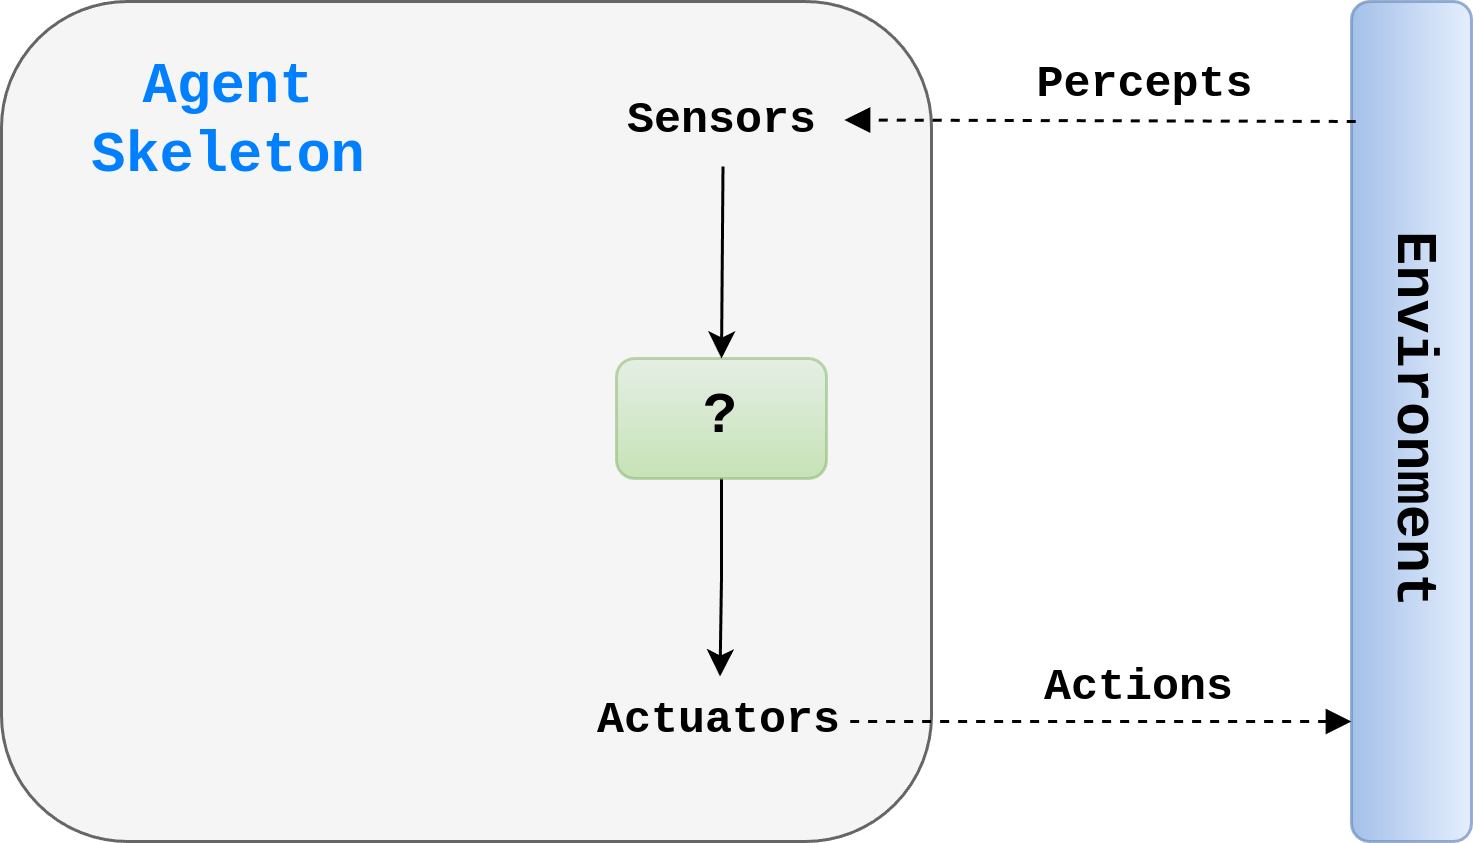
\includegraphics[
        width=0.5\linewidth,
        height=4cm,
        keepaspectratio
    ]{images/artificial-intelligence/ai-agents/agents-skeleton.png}
    \caption*{Agents interact with environments through sensors and actuators. \cite{common/online/tools/draw.io}}
\end{figure}


\begin{enumerate}
    \item \textbf{Agent}: An agent is anything that can be viewed as perceiving its environment through sensors and acting upon that environment through actuators.
    \hfill \cite{ai/book/Artificial-Intelligence-A-Modern-Approach/Russell-Norvig}
    \\
    \verb|agent = architecture + (agent) program|
    \hfill \cite{ai/book/Artificial-Intelligence-A-Modern-Approach/Russell-Norvig}

    \item \textbf{Environment}: environment refers to everything outside the agent that it interacts with.
    \hfill \cite{common/online/chatgpt}
    \\
    The “geography” of the environment is known \textbf{a priori}.
    \hfill \cite{ai/book/Artificial-Intelligence-A-Modern-Approach/Russell-Norvig}
    \\
    "A priori" : Knowledge or assumptions made before data is observed (e.g., predefined rules, constraints).
    \hfill \cite{common/online/chatgpt}

    \item \textbf{Sensors}: A sensor is any mechanism that allows an AI agent to perceive its environment by gathering information. This can be physical (hardware) or virtual (software).
    \hfill \cite{common/online/chatgpt}

    \item \textbf{Actuators}: An actuator is any mechanism that allows an AI agent to affect or change its environment by performing actions.
    \hfill \cite{common/online/chatgpt}

    \item \textbf{Percept}: agent’s perceptual inputs at any given instant
    \hfill \cite{ai/book/Artificial-Intelligence-A-Modern-Approach/Russell-Norvig}

    \item \textbf{Percept Sequence}: it is the complete history of everything the agent has ever perceived. In general, an agent’s choice of action at any given instant can depend on the entire percept sequence observed to date, but \textbf{not} on anything it hasn’t perceived.
    \hfill \cite{ai/book/Artificial-Intelligence-A-Modern-Approach/Russell-Norvig}

    \item \textbf{Agent Function}: maps any given percept sequence to an action; describes agent’s behavior; an external characterization of the agent; The agent function is an abstract mathematical description; takes the entire percept history
    \hfill \cite{ai/book/Artificial-Intelligence-A-Modern-Approach/Russell-Norvig}

    \item \textbf{Agent Program}: internal implementation of the agent function for an artificial agent; the agent program is a concrete implementation, running within some physical system. The agent program takes just the current percept as input because nothing more is available from the environment; if the agent’s actions need to depend on the entire percept sequence, the agent will have to remember the percepts.
    \hfill \cite{ai/book/Artificial-Intelligence-A-Modern-Approach/Russell-Norvig}

    \item \textbf{Architecture}: computing device with physical sensors and actuators on which the agent program is running.
    \hfill \cite{ai/book/Artificial-Intelligence-A-Modern-Approach/Russell-Norvig}

    \item \textbf{Performance Measure}: It evaluates any given sequence of environment states.
    \hfill \cite{ai/book/Artificial-Intelligence-A-Modern-Approach/Russell-Norvig}

    \item \textbf{Rational Agent}: A rational agent is one that does the right thing
    \hfill \cite{ai/book/Artificial-Intelligence-A-Modern-Approach/Russell-Norvig}
    \\
    For each possible percept sequence, a rational agent should select an action that is expected to maximize its performance measure, given the evidence provided by the percept sequence and whatever built-in knowledge the agent has.
    \hfill \cite{ai/book/Artificial-Intelligence-A-Modern-Approach/Russell-Norvig}
    \\
    Rationality is not the same as perfection.
    \hfill \cite{ai/book/Artificial-Intelligence-A-Modern-Approach/Russell-Norvig}
    \\
    Rationality maximizes \textbf{expected} performance, while perfection maximizes \textbf{actual} performance.
    \hfill \cite{ai/book/Artificial-Intelligence-A-Modern-Approach/Russell-Norvig}
    \\
    Our definition of rationality does not require omniscience, then, because the rational choice depends only on the percept sequence to date
    \hfill \cite{ai/book/Artificial-Intelligence-A-Modern-Approach/Russell-Norvig}


    \item \textbf{Omniscient Agent}: An omniscient agent knows the actual outcome of its actions and can act accordingly; but omniscience is impossible in reality.
    \hfill \cite{ai/book/Artificial-Intelligence-A-Modern-Approach/Russell-Norvig}


    \item \textbf{Information Gathering}: It is doing actions in order to modify future percepts.
    \hfill \cite{ai/book/Artificial-Intelligence-A-Modern-Approach/Russell-Norvig}



    \item When an agent is plunked down in an environment, it generates a sequence of actions according to the percepts it receives. This sequence of actions causes the environment to go through a sequence of states. If the sequence is desirable, then the agent has performed well.
    \hfill \cite{ai/book/Artificial-Intelligence-A-Modern-Approach/Russell-Norvig}

    \item  If we define success in terms of agent’s opinion of its own performance, an agent could achieve perfect rationality simply by deluding itself that its performance was perfect.
    \hfill \cite{ai/book/Artificial-Intelligence-A-Modern-Approach/Russell-Norvig}

    \item Human agents in particular are notorious for “sour grapes” - believing they did not really want something (e.g., a Nobel Prize) after not getting it.
    \hfill \cite{ai/book/Artificial-Intelligence-A-Modern-Approach/Russell-Norvig}

    \item As a general rule, it is better to design performance measures according to what one actually wants in the environment, rather than according to how one thinks the agent should behave.
    \hfill \cite{ai/book/Artificial-Intelligence-A-Modern-Approach/Russell-Norvig}

    \item The agent’s initial configuration could reflect some prior knowledge of the environment, but as the agent gains experience this may be modified and augmented. There are extreme cases in which the environment is completely known \textbf{a priori}. In such cases, the agent need not perceive or learn; it simply acts correctly. Such agents are fragile.
    \hfill \cite{ai/book/Artificial-Intelligence-A-Modern-Approach/Russell-Norvig}

    \item To the extent that an agent relies on the prior knowledge of its designer rather than on its own percepts, we say that the agent \textbf{lacks autonomy}.
    \hfill \cite{ai/book/Artificial-Intelligence-A-Modern-Approach/Russell-Norvig}
    \\
    A rational agent should be \textbf{autonomous} - it should learn what it can to compensate for partial or incorrect prior knowledge.
    \hfill \cite{ai/book/Artificial-Intelligence-A-Modern-Approach/Russell-Norvig}

    \item After sufficient experience of its environment, the behavior of a rational agent can become effectively \textbf{independent} of its prior knowledge. Hence, the incorporation of learning allows one to design a single rational agent that will succeed in a vast variety of environments.
    \hfill \cite{ai/book/Artificial-Intelligence-A-Modern-Approach/Russell-Norvig}


\end{enumerate}




\section{Task Environment/ Problem \cite{ai/book/Artificial-Intelligence-A-Modern-Approach/Russell-Norvig}}\label{AI: Agents/Task Environment or Problem}


\begin{enumerate}
    \item Task environments are essentially the “problems” to which rational agents are the “solutions.”
    \hfill \cite{ai/book/Artificial-Intelligence-A-Modern-Approach/Russell-Norvig}


\end{enumerate}

\subsection{PEAS: Defining Problem}

\begin{enumerate}
    \item \textbf{Performance}:
    \begin{enumerate}
        \item Desirable qualities
        \hfill \cite{ai/book/Artificial-Intelligence-A-Modern-Approach/Russell-Norvig}

        \item Defines how the success of the agent is evaluated.
        \hfill \cite{common/online/chatgpt}

        \item[] \textbf{Example}: In a self-driving car, performance can be measured by safety, fuel efficiency, and reaching the destination on time.
        \hfill \cite{common/online/chatgpt}
    \end{enumerate}

    \item \textbf{Environment}:
    \begin{enumerate}
        \item The surroundings in which the agent operates.
        \hfill \cite{common/online/chatgpt}

        \item[] \textbf{Example}: For a self-driving car, the environment includes roads, traffic, pedestrians, and weather conditions.
        \hfill \cite{common/online/chatgpt}
    \end{enumerate}

    \item \textbf{Actuators}:
    \begin{enumerate}
        \item The mechanisms that allow the agent to take action.
        \hfill \cite{common/online/chatgpt}

        \hfill Can be hardware or software.

        \item[] \textbf{Example}: A self-driving car uses its steering wheel, accelerator, and brakes as actuators.
        \hfill \cite{common/online/chatgpt}
    \end{enumerate}

    \item \textbf{Sensors}:
    \begin{enumerate}
        \item The components that allow the agent to perceive its environment.
        \hfill \cite{common/online/chatgpt}

        \hfill Can be hardware or software.

        \item[] \textbf{Example}: A self-driving car has cameras, LiDAR, GPS, and speed sensors.
        \hfill \cite{common/online/chatgpt}
    \end{enumerate}

\end{enumerate}


\vspace{0.3cm}

\textbf{Note}:
\begin{enumerate}
    \item some \textbf{software agents} (or \textbf{software robots} or \textbf{softbots}) exist in rich, unlimited domains.
    \hfill \cite{ai/book/Artificial-Intelligence-A-Modern-Approach/Russell-Norvig}


\end{enumerate}


\clearpage
\subsection{Properties of Task Environments \cite{ai/book/Artificial-Intelligence-A-Modern-Approach/Russell-Norvig}}

\subsubsection{Fully observable, partially observable, unobservable}
\begin{enumerate}
    \item \textbf{fully observable}: If an agent’s sensors give it access to the complete state of the environment at each point in time, then we say that the task environment is fully observable.
    A task environment is effectively fully observable if the sensors detect all aspects that are \textbf{relevant} to the choice of action; relevance, in turn, depends on the performance measure.
    Fully observable environments are convenient because the agent need not maintain any internal state to keep track of the world.
    \hfill \cite{ai/book/Artificial-Intelligence-A-Modern-Approach/Russell-Norvig}

    \vspace{0.2cm}

    \item \textbf{partially observable}: An environment might be partially observable because of noisy and inaccurate sensors or because parts of the state are simply missing from the sensor data.
    \hfill \cite{ai/book/Artificial-Intelligence-A-Modern-Approach/Russell-Norvig}

    \vspace{0.2cm}

    \item \textbf{unobservable}: If the agent has no sensors at all then the environment is unobservable.
    The agent’s goals may still be achievable, sometimes with certainty.
    \hfill \cite{ai/book/Artificial-Intelligence-A-Modern-Approach/Russell-Norvig}
\end{enumerate}

\subsubsection{Single agent, multi-agent}
\begin{enumerate}
    \item \textbf{Single agent}:  Only 1 agent is interacting in the given environment.

    \item \textbf{Multi-agent}: More than 1 agent (of same type or different types) interact in the given environment.
    \begin{enumerate}
        \item \textbf{Competitive Multi-agent}: Agents maximize their own performance at cost of other agents' performance.
        \\
        Examples: 2 agents playing Chess against each other; taxi-driving (competing for parking space)

        \item \textbf{Cooperative Multi-agent}: Agents take actions to maximize collective performance.
        \\
        Example: taxi-driving (avoiding collisions)

        \vspace{0.3cm}

        \item \textbf{communication} often emerges as a rational behavior in multiagent environments; in some competitive environments, \textbf{randomized behavior} is rational because it avoids the pitfalls of predictability.
        \hfill \cite{ai/book/Artificial-Intelligence-A-Modern-Approach/Russell-Norvig}
    \end{enumerate}

\end{enumerate}


\subsubsection{Deterministic, stochastic, uncertain, nondeterministic}
\begin{enumerate}
    \item If the next state of the environment is completely determined by the current state and the action executed by the agent, then we say the environment is \textbf{deterministic}; otherwise, it is \textbf{stochastic}.
    \hfill \cite{ai/book/Artificial-Intelligence-A-Modern-Approach/Russell-Norvig}

    \item In principle, an agent need not worry about uncertainty in a fully observable, deterministic environment.
    \hfill \cite{ai/book/Artificial-Intelligence-A-Modern-Approach/Russell-Norvig}

    \item  If the environment is partially observable, however, then it could appear to be stochastic. Most real situations are so complex that it is impossible to keep track of all the unobserved aspects; for practical purposes, they must be treated as \textbf{stochastic}.
    \hfill \cite{ai/book/Artificial-Intelligence-A-Modern-Approach/Russell-Norvig}
    \\
    It implies that uncertainty about outcomes is quantified in terms of \textit{probabilities}.
    \hfill \cite{ai/book/Artificial-Intelligence-A-Modern-Approach/Russell-Norvig}

    \item  We say an environment is \textbf{uncertain} if it is not fully observable or not deterministic.
    \hfill \cite{ai/book/Artificial-Intelligence-A-Modern-Approach/Russell-Norvig}

    \item A \textbf{nondeterministic} environment is one in which actions are characterized by their possible outcomes, but no probabilities are attached to them. Non-deterministic environment descriptions are usually associated with performance measures that require the agent to succeed for all possible outcomes of its actions.
    \hfill \cite{ai/book/Artificial-Intelligence-A-Modern-Approach/Russell-Norvig}
\end{enumerate}


\subsubsection{Episodic, sequential}
\begin{enumerate}
    \item In an \textbf{episodic} task environment, the agent’s experience is divided into atomic episodes. In each episode the agent receives a percept and then performs a single action. Crucially, the next episode does not depend on the actions taken in previous episodes. Episodic environments are much simpler than sequential environments because the agent does not need to think ahead.
    \hfill \cite{ai/book/Artificial-Intelligence-A-Modern-Approach/Russell-Norvig}

    \item In \textbf{sequential} environments, on the other hand, the current decision could affect all future decisions.
    \hfill \cite{ai/book/Artificial-Intelligence-A-Modern-Approach/Russell-Norvig}
\end{enumerate}


\subsubsection{Static, dynamic, semidynamic}
\begin{enumerate}
    \item If the environment can change while an agent is deliberating, then we say the environment is \textbf{dynamic} for that agent; otherwise, it is \textbf{static}.
    \hfill \cite{ai/book/Artificial-Intelligence-A-Modern-Approach/Russell-Norvig}

    \item Static environments are easy to deal with because the agent need not keep looking at the world while it is deciding on an action, nor need it worry about the passage of time.
    \hfill \cite{ai/book/Artificial-Intelligence-A-Modern-Approach/Russell-Norvig}

    \item  Dynamic environments, on the other hand, are continuously asking the agent what it wants to do; if it hasn’t decided yet, that counts as deciding to do nothing.
    \hfill \cite{ai/book/Artificial-Intelligence-A-Modern-Approach/Russell-Norvig}

    \item If the environment itself does not change with the passage of time but the agent’s performance score does, then we say the environment is \textbf{semidynamic}.
    \hfill \cite{ai/book/Artificial-Intelligence-A-Modern-Approach/Russell-Norvig}
\end{enumerate}


\subsubsection{Discrete, continuous}
\begin{enumerate}
    \item The discrete/continuous distinction applies to the state of the environment, to the way \textit{time} is handled, and to the percepts and actions of the agent.
    \hfill \cite{ai/book/Artificial-Intelligence-A-Modern-Approach/Russell-Norvig}


\end{enumerate}



\subsubsection{Known, unknown}
\begin{enumerate}
    \item Strictly speaking, this distinction refers not to the environment itself but to the agent’s (or designer’s) state of knowledge about the “laws of physics” of the environment.
    \hfill \cite{ai/book/Artificial-Intelligence-A-Modern-Approach/Russell-Norvig}

    \item In a \textbf{known} environment, the outcomes (or outcome probabilities if the environment is stochastic) for all actions are given.
    \hfill \cite{ai/book/Artificial-Intelligence-A-Modern-Approach/Russell-Norvig}

    \item  if the environment is \textbf{unknown}, the agent will have to learn how it works in order to make good decisions.
    \hfill \cite{ai/book/Artificial-Intelligence-A-Modern-Approach/Russell-Norvig}


\end{enumerate}



\subsubsection*{Examples \cite{ai/book/Artificial-Intelligence-A-Modern-Approach/Russell-Norvig}}

\begin{customArrayStretch}{1.3}
\begin{tabular}{ | >{\fontsize{10}{10}\arraybackslash}l | l l l l l l | }
    \hline

    \textbf{Task Environment} & \textbf{Observable} & \textbf{Agents} &
        \textbf{Deterministic} & \textbf{Episodic} &
        \textbf{Static} & \textbf{Discrete} \\

    \hline\hline

    \textbf{Crossword puzzle} & Fully & Single & Deterministic & Sequential & Static & Discrete \\

    \textbf{Chess with a clock} & Fully & Multi & Deterministic & Sequential & Semi & Discrete \\

    \hline

    \textbf{Poker} & Partially & Multi & Stochastic & Sequential & Static & Discrete \\

    \textbf{Backgammon} & Fully & Multi & Stochastic & Sequential & Static & Discrete \\

    \hline

    \textbf{Taxi driving} & Partially & Multi & Stochastic & Sequential & Dynamic & Continuous \\

    \textbf{Medical diagnosis} & Partially & Single & Stochastic & Sequential & Dynamic & Continuous \\

    \hline

    \textbf{Image analysis} & Fully & Single & Deterministic & Episodic & Semi & Continuous \\

    \textbf{Part-picking robot} & Partially & Single & Stochastic & Episodic & Dynamic & Continuous \\

    \hline

    \textbf{Refinery controller} & Partially & Single & Stochastic & Sequential & Dynamic & Continuous \\

    \textbf{Interactive English tutor} & Partially & Multi & Stochastic & Sequential & Dynamic & Discrete \\

    \hline
\end{tabular}
\end{customArrayStretch}



\subsubsection*{Note}
\begin{enumerate}
    \item  the distinction between known and unknown environments is not the same as the one between fully and partially observable environments.
    \hfill \cite{ai/book/Artificial-Intelligence-A-Modern-Approach/Russell-Norvig}

    \item It is quite possible for a \textbf{known} environment to be \textbf{partially observable}—for example, in solitaire card games, I know the rules but am still unable to see the cards that have not yet been turned over.
    \hfill \cite{ai/book/Artificial-Intelligence-A-Modern-Approach/Russell-Norvig}

    \item an \textbf{unknown} environment can be \textbf{fully observable}—in a new video game, the screen may show the entire game state but I still don’t know what the buttons do until I try them.
    \hfill \cite{ai/book/Artificial-Intelligence-A-Modern-Approach/Russell-Norvig}

    \item \textbf{environment class}: A category or set of related environments from which specific environments are drawn for testing or training agents.
    \hfill \cite{ai/book/Artificial-Intelligence-A-Modern-Approach/Russell-Norvig, common/online/chatgpt}

    \item \textbf{environment generator}: An environment generator is a tool or function that creates individual environments sampled from an environment class. It automates the creation of diverse scenarios for training or evaluating agents.
    \hfill \cite{ai/book/Artificial-Intelligence-A-Modern-Approach/Russell-Norvig, common/online/chatgpt}


\end{enumerate}



\section{Agent State Representations}\label{AI: Agents/Agent State Representations}

\begin{figure}[H]
    \centering
    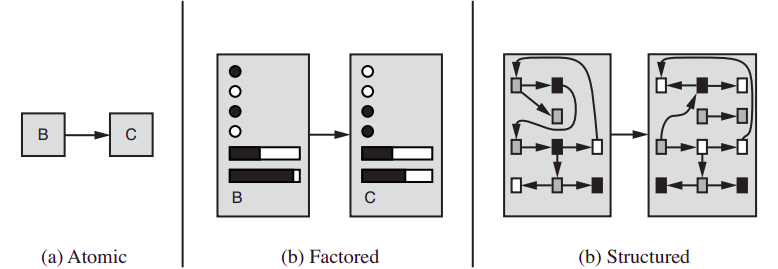
\includegraphics[
        width=\linewidth,
        height=6cm,
        keepaspectratio,
    ]{images/artificial-intelligence/ai-agents/state-representations.png}
    \caption*{
    Three ways to represent states and the transitions between them.
    \\
    \textbf{(a)} Atomic representation: a state (such as B or C) is a black box with no internal structure;  
    \hfill \cite{ai/book/Artificial-Intelligence-A-Modern-Approach/Russell-Norvig}
    \\
    \textbf{(b)} Factored representation: a state consists of a vector of attribute values; values can be Boolean, realvalued, or one of a fixed set of symbols.
    \hfill \cite{ai/book/Artificial-Intelligence-A-Modern-Approach/Russell-Norvig}
    \\
    \textbf{(c)} Structured representation: a state includes objects, each of which may have attributes of its own as well as relationships to other objects.
    \hfill \cite{ai/book/Artificial-Intelligence-A-Modern-Approach/Russell-Norvig}
}
\end{figure}



\begin{enumerate}[itemsep=0.2cm]
    \item Roughly speaking, a more expressive representation can capture, at least as concisely, everything a less expressive one can capture, plus some more. 
    \hfill \cite{ai/book/Artificial-Intelligence-A-Modern-Approach/Russell-Norvig}

    \item Often, the more expressive language is much more concise; for example, the rules of chess can be written in a page or two of a structured-representation language such as first-order logic but require thousands of pages when written in a factored-representation language such as propositional logic.
    \hfill \cite{ai/book/Artificial-Intelligence-A-Modern-Approach/Russell-Norvig}

    \item reasoning and learning become more complex as the expressive power of the representation increases.
    \hfill \cite{ai/book/Artificial-Intelligence-A-Modern-Approach/Russell-Norvig}

    \item To gain the benefits of expressive representations while avoiding their drawbacks, intelligent systems for the real world may need to operate at all points along the axis simultaneously.
    \hfill \cite{ai/book/Artificial-Intelligence-A-Modern-Approach/Russell-Norvig}
\end{enumerate}






\subsection{Atomic representation}

\begin{enumerate}[itemsep=0.2cm]
    \item each state of the world is indivisible - it has no internal structure. 
    \hfill \cite{ai/book/Artificial-Intelligence-A-Modern-Approach/Russell-Norvig}

    \item two different atomic states have nothing in common—they are just different black boxes
    \hfill \cite{ai/book/Artificial-Intelligence-A-Modern-Approach/Russell-Norvig}

    \item Algorithms/ areas that work with atomic representations - or, at least, they treat representations as if they were atomic:
    \begin{enumerate}
        \item Search and game-playing
        \hfill \cite{ai/book/Artificial-Intelligence-A-Modern-Approach/Russell-Norvig}

        \item Hidden Markov models
        \hfill \cite{ai/book/Artificial-Intelligence-A-Modern-Approach/Russell-Norvig}

        \item Markov decision processes
        \hfill \cite{ai/book/Artificial-Intelligence-A-Modern-Approach/Russell-Norvig}
    \end{enumerate}
\end{enumerate}



\subsection{Factored representation}

\begin{enumerate}[itemsep=0.2cm]
    \item A factored representation splits up each state into a fixed set of \textbf{variables} or \textbf{attributes}, each of which can have a \textbf{value}.
    \hfill \cite{ai/book/Artificial-Intelligence-A-Modern-Approach/Russell-Norvig}

    \item two different factored states can \textbf{share} some attributes (such as being at some particular GPS location) and not others (such as having lots of gas or having no gas)
    \\
    this makes it much easier to work out how to turn one state into another
    \hfill \cite{ai/book/Artificial-Intelligence-A-Modern-Approach/Russell-Norvig}

    \item With factored representations, we can also represent uncertainty - for example, ignorance about the amount of gas in the tank can be represented by leaving that attribute blank.
    \hfill \cite{ai/book/Artificial-Intelligence-A-Modern-Approach/Russell-Norvig}

    \item Algorithms/ areas based on factored representations:
    \begin{enumerate}
        \item constraint satisfaction algorithms
        \hfill \cite{ai/book/Artificial-Intelligence-A-Modern-Approach/Russell-Norvig}

        \item propositional logic
        \hfill \cite{ai/book/Artificial-Intelligence-A-Modern-Approach/Russell-Norvig}

        \item planning
        \hfill \cite{ai/book/Artificial-Intelligence-A-Modern-Approach/Russell-Norvig}

        \item Bayesian networks
        \hfill \cite{ai/book/Artificial-Intelligence-A-Modern-Approach/Russell-Norvig}

    \end{enumerate}
\end{enumerate}








\subsection{Structured representation}


\begin{enumerate}[itemsep=0.2cm]
    \item the world as having things in it that are related to each other, not just variables with values.
    \hfill \cite{ai/book/Artificial-Intelligence-A-Modern-Approach/Russell-Norvig}

    \item almost everything that humans express in natural language concerns objects and their relationships
    \hfill \cite{ai/book/Artificial-Intelligence-A-Modern-Approach/Russell-Norvig}

    \item Algorithms/ areas based on factored representations:
    \begin{enumerate}
        \item relational databases
        \hfill \cite{ai/book/Artificial-Intelligence-A-Modern-Approach/Russell-Norvig}

        \item first-order logic
        \hfill \cite{ai/book/Artificial-Intelligence-A-Modern-Approach/Russell-Norvig}

        \item first-order probability models 
        \hfill \cite{ai/book/Artificial-Intelligence-A-Modern-Approach/Russell-Norvig}

        \item knowledge-based learning
        \hfill \cite{ai/book/Artificial-Intelligence-A-Modern-Approach/Russell-Norvig}

        \item natural language understanding
        \hfill \cite{ai/book/Artificial-Intelligence-A-Modern-Approach/Russell-Norvig}
    \end{enumerate}
\end{enumerate}






\chapter{AI: Agent Programs}


\section{Table Driven Agent}\label{AI: Agent Programs/Table Driven Agent}


\begin{figure}[H]
    \centering
    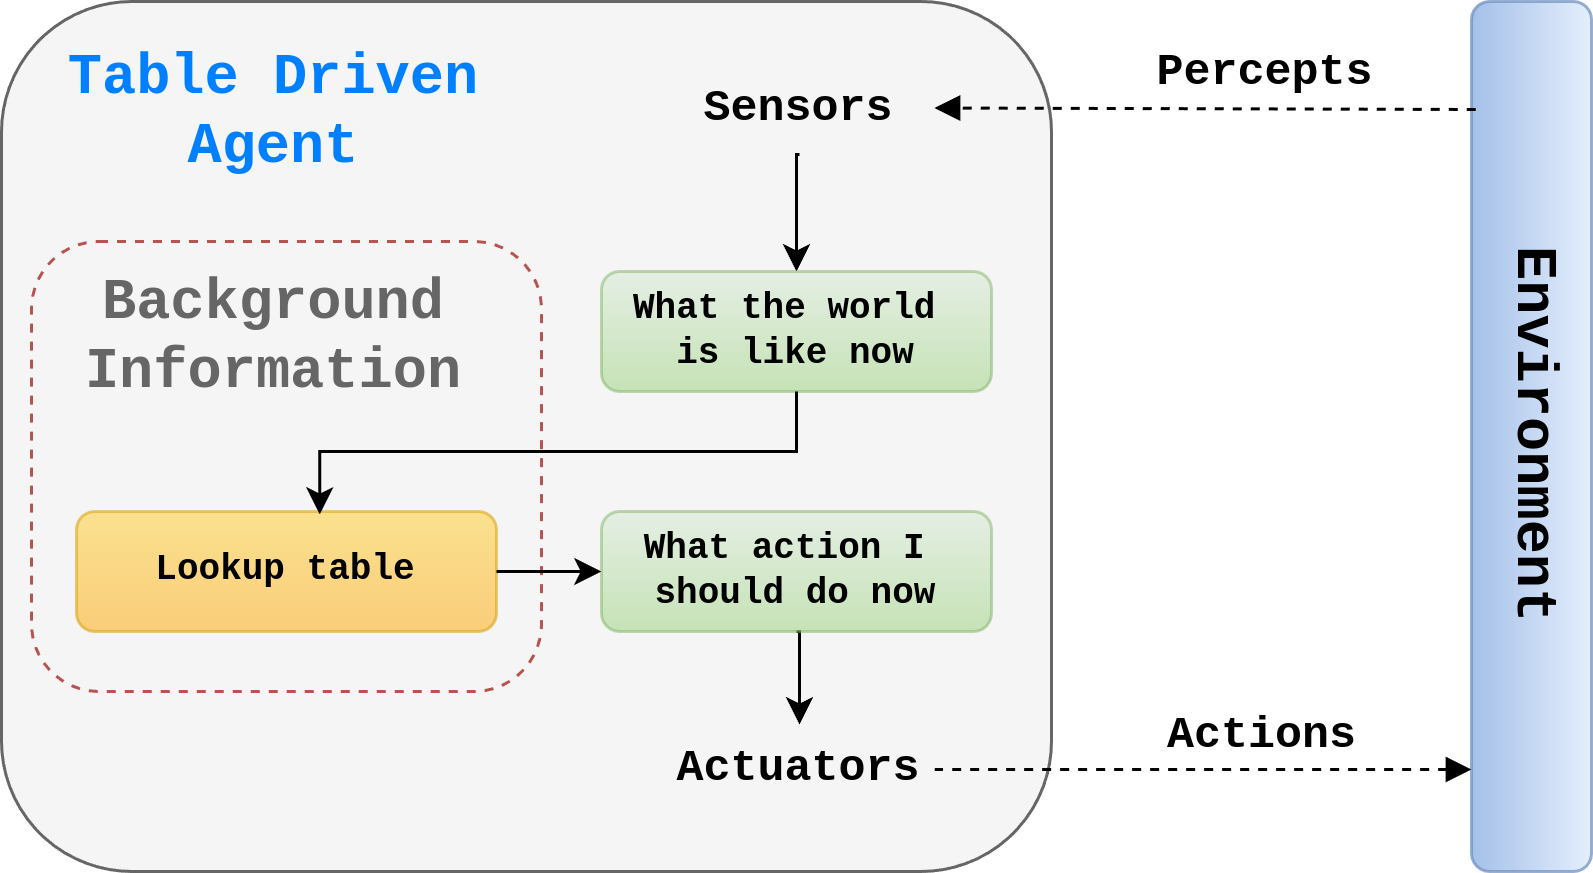
\includegraphics[
        width=0.5\linewidth,
        height=4cm,
        keepaspectratio
    ]{images/artificial-intelligence/ai-agents/agents-table-driven-agent.png}
    \caption*{Schematic diagram of a table driven agent. \cite{common/online/tools/draw.io}}
\end{figure}

\begin{longtable}{l l}

$\mathcal{P}$ & set of possible percepts \\

$T$ & lifetime of agent (total number of percepts) \\

\end{longtable}


\vspace{0.5cm}

\begin{enumerate}
    \item Number of entries in table: $
        \dsum_{t=1}^T \dabs{\mathcal{P}}^t
    $
    \hfill \cite{ai/book/Artificial-Intelligence-A-Modern-Approach/Russell-Norvig}

    \item Sometimes the number of entries can be ridiculously large number due to the combinations of percepts and length of percept sequence.\\
    \textbf{Example}: Consider the \textit{automated taxi}: the visual input from a single camera comes in at the rate of roughly $27$ megabytes per second ($30$ frames per second, $640 \times 480$ pixels with $24$ bits of color information). This gives a lookup table with over $10^{250,000,000,000}$ entries for an hour’s driving.
    \hfill \cite{ai/book/Artificial-Intelligence-A-Modern-Approach/Russell-Norvig}
    \\
    It means:
    \begin{enumerate}
        \item no physical agent in this universe will have the space to store the table
        \hfill \cite{ai/book/Artificial-Intelligence-A-Modern-Approach/Russell-Norvig}

        \item the designer would not have time to create the table
        \hfill \cite{ai/book/Artificial-Intelligence-A-Modern-Approach/Russell-Norvig}

        \item no agent could ever learn all the right table entries from its experience
        \hfill \cite{ai/book/Artificial-Intelligence-A-Modern-Approach/Russell-Norvig}

        \item even if the environment is simple enough to yield a feasible table size, the designer still has no guidance about how to fill in the table entries
        \hfill \cite{ai/book/Artificial-Intelligence-A-Modern-Approach/Russell-Norvig}

    \end{enumerate}
\end{enumerate}

\vspace{0.5cm}

\begin{algorithm}[H]
    \caption{The \textsc{Table-Driven-Agent} program is invoked for each new percept and returns an action each time. It retains the complete percept sequence in memory. \cite{ai/book/Artificial-Intelligence-A-Modern-Approach/Russell-Norvig}}

    \SetKwFunction{FUNCTION}{\textsc{Table-Driven-Agent}}
    \SetKwProg{Fn}{function}{ returns \normalfont an action}{end}
    \Fn{\FUNCTION{ percept }}{
        \textbf{persistent}:\\

        \hspace{0.4cm} $percepts$, a sequence, initially empty\\

        \hspace{0.4cm} $table$, a table of actions, indexed by percept sequences, initially fully specified \\

        \ \\

        append $percept$ to the end of $percepts$ \\

        $action$ $\gets$ \textsc{Lookup}($\ percepts,\ table\ $) \\

        \Return $action$
    }
\end{algorithm}





\section{Simple Reflex Agent}\label{AI: Agent Programs/Simple Reflex Agent}


\begin{figure}[H]
    \centering
    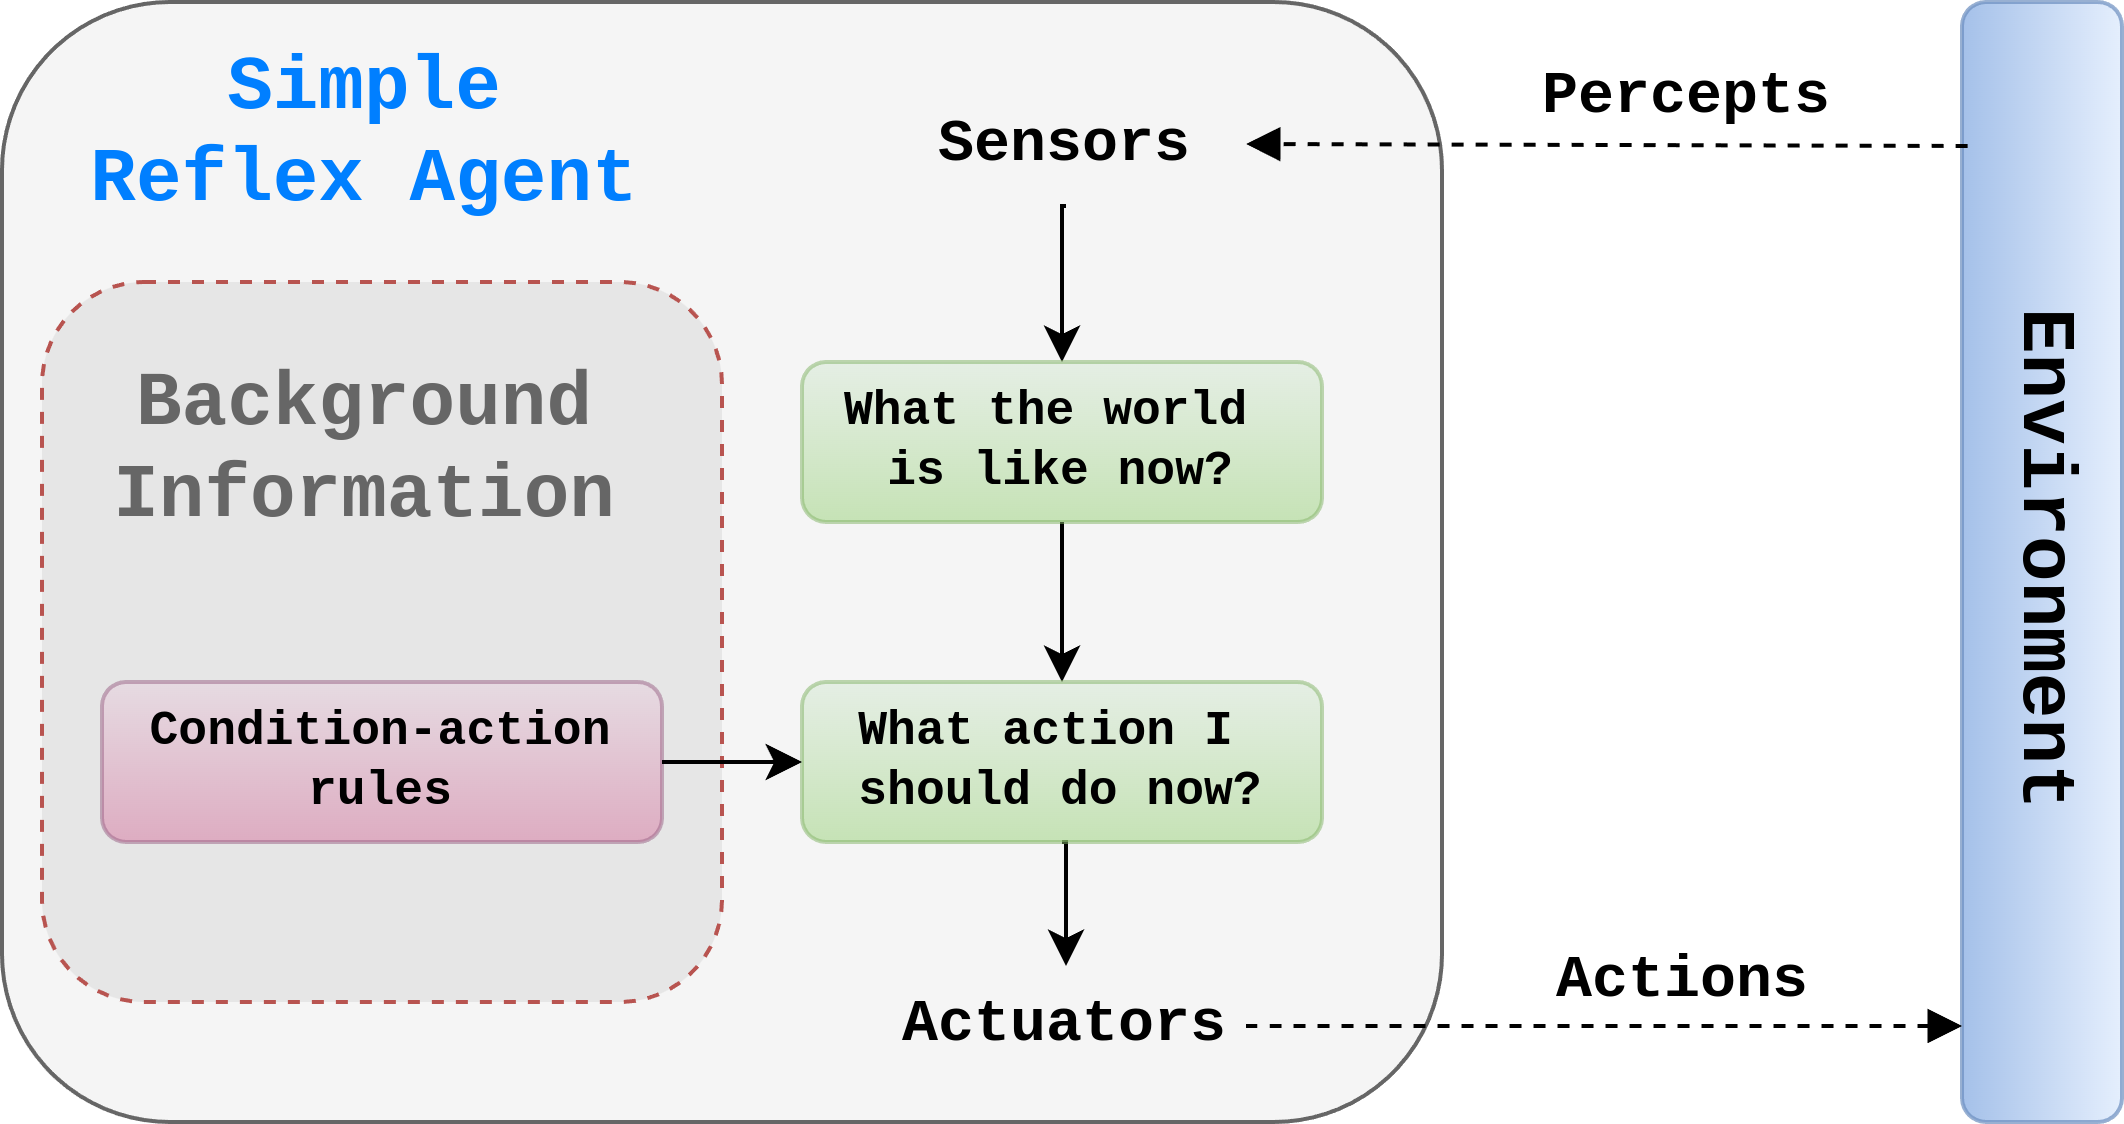
\includegraphics[
        width=0.5\linewidth, 
        height=4cm, 
        keepaspectratio
    ]{images/artificial-intelligence/ai-agents/agents-Simple-reflex-agent.png}
    \caption*{Schematic diagram of a simple reflex agent. \cite{common/online/tools/draw.io}}
\end{figure}

\begin{enumerate}
    \item simplest kind of agent
    \hfill \cite{ai/book/Artificial-Intelligence-A-Modern-Approach/Russell-Norvig}

    \item These agents select actions on the basis of the \textit{current} percept, ignoring the rest of the percept history.
    \hfill \cite{ai/book/Artificial-Intelligence-A-Modern-Approach/Russell-Norvig}

    \item \textbf{condition-action rule/ situation-action rules/ productions/ if-then rules}:\\
    A condition-action rule is a basic decision-making structure used in reflex agents and rule-based systems.
    \hfill \cite{ai/book/Artificial-Intelligence-A-Modern-Approach/Russell-Norvig, common/online/chatgpt}

    \item the description in terms of “rules” and “matching” is purely conceptual; actual implementations can be as simple as a collection of logic gates implementing a Boolean circuit.
    \hfill \cite{ai/book/Artificial-Intelligence-A-Modern-Approach/Russell-Norvig}

    \item Escape from infinite loops is possible if the agent can \textbf{randomize} its actions.  
    A randomized simple reflex agent \textit{might outperform} a deterministic simple reflex agent.
    Randomized behavior of the right kind can be rational in some multi-agent environments. 
    In single-agent environments, randomization is usually \textbf{not} rational. 
    \hfill \cite{ai/book/Artificial-Intelligence-A-Modern-Approach/Russell-Norvig}
    

    \item \textbf{Disadvantage}: limited intelligence
    \hfill \cite{ai/book/Artificial-Intelligence-A-Modern-Approach/Russell-Norvig}

    \item \textbf{Disadvantage}: will work only if the correct decision can be made on the basis of only the current percept—that is, only if the environment is fully observable. Even a little bit of un-observability can cause serious trouble.
    \hfill \cite{ai/book/Artificial-Intelligence-A-Modern-Approach/Russell-Norvig}

    \item \textbf{Disadvantage}: we would have to rewrite many condition–action rules for supporting more situations/ scenarios. 

\end{enumerate}


\vspace{0.5cm}


\begin{algorithm}[H]
    \caption{\textsc{Simple-Reflex-Agent}: It acts according to a rule whose condition matches the current state, as defined by the percept. \cite{ai/book/Artificial-Intelligence-A-Modern-Approach/Russell-Norvig}}

    \SetKwFunction{FUNCTION}{\textsc{Simple-Reflex-Agent}}
    \SetKwProg{Fn}{function}{ returns \normalfont an action}{end}
    \Fn{\FUNCTION{ percept }}{
        \textbf{persistent}: $rules$, a set of condition-action rules \\
        \ \\
        $state$ $\gets$ \textsc{Interpret-Input}( $percept$ )\\
        $rule$ $\gets$ \textsc{Rule-Match}( $state,\ rules$ ) \\
        $action$ $\gets$ $rule$.\textsc{Action} \\
        \Return $action$
    }
\end{algorithm}

\vspace{0.3cm}

\begin{customArrayStretch}{1.2}
\begin{longtable}{l p{12cm} l}

\textsc{Interpret-Input} & 
    generates an abstracted description of the current state from the percept &
    \cite{ai/book/Artificial-Intelligence-A-Modern-Approach/Russell-Norvig} \\

\textsc{Rule-Match} & 
    returns the first rule in the set of rules that matches the given state description &
    \cite{ai/book/Artificial-Intelligence-A-Modern-Approach/Russell-Norvig} \\

\end{longtable}
\end{customArrayStretch}










\section{Model-based reflex agents}\label{AI: Agent Programs/Model-based reflex agents}


\begin{figure}[H]
    \centering
    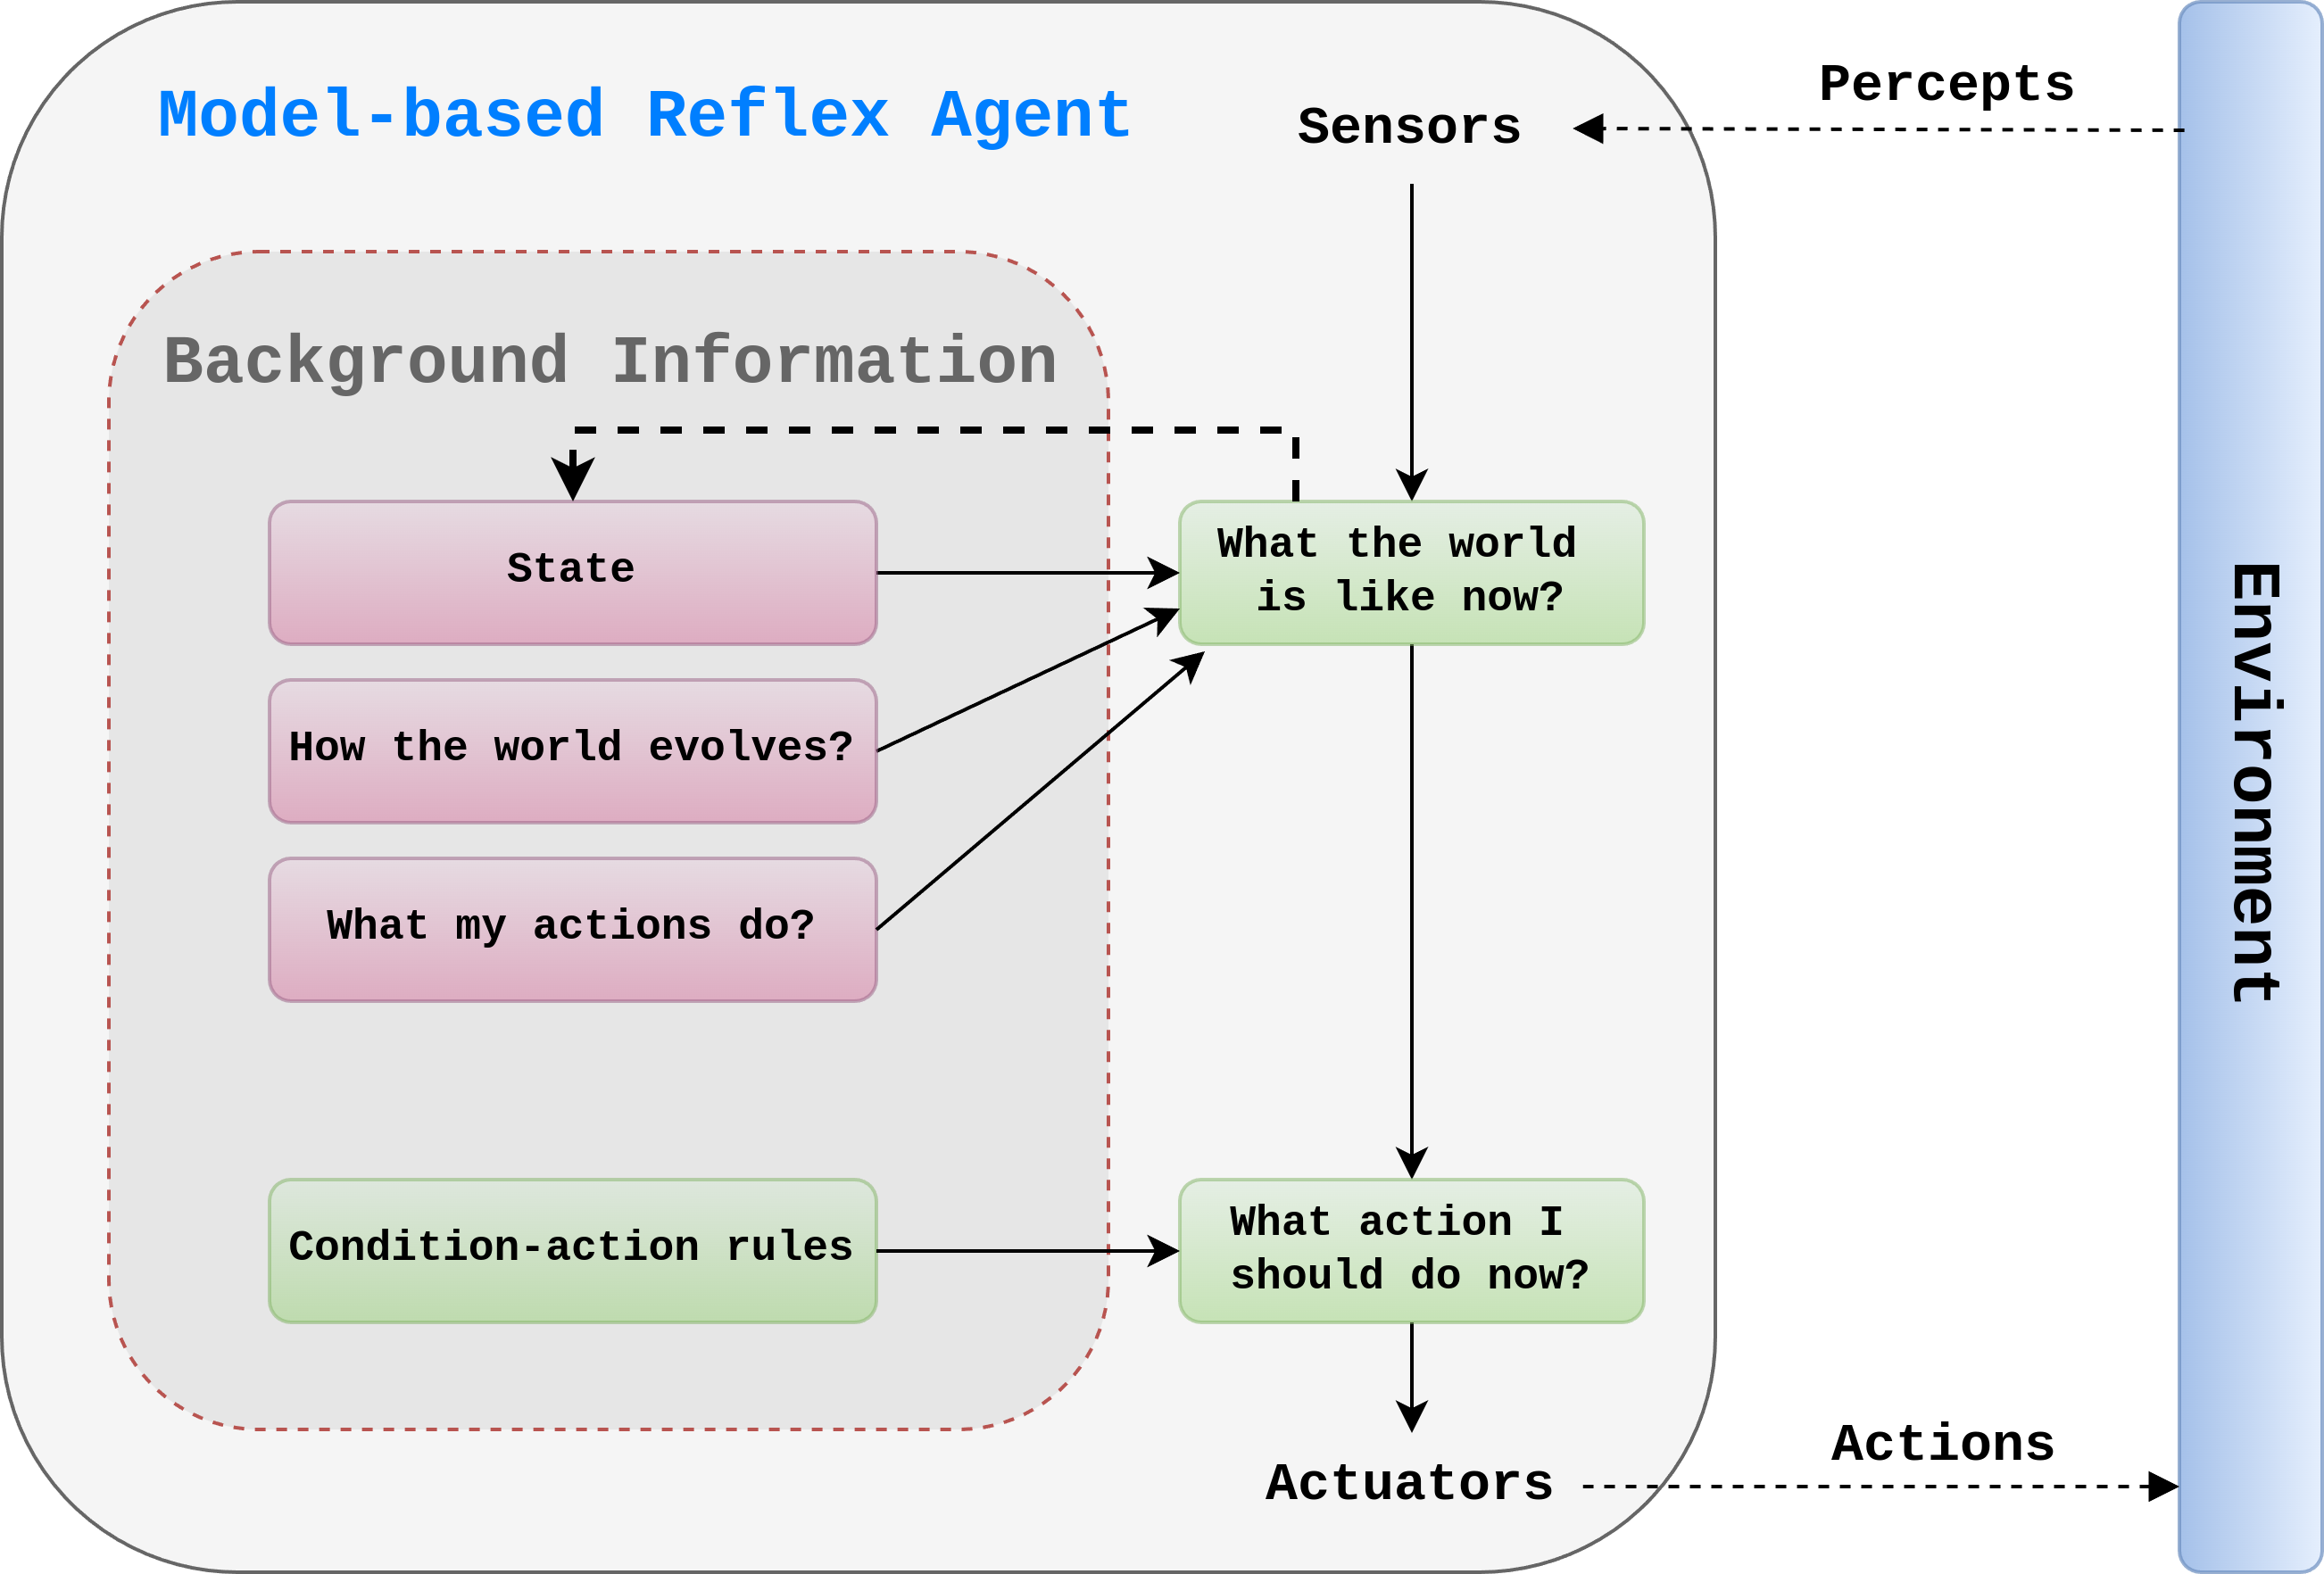
\includegraphics[
        width=0.5\linewidth, 
        height=6cm, 
        keepaspectratio
    ]{images/artificial-intelligence/ai-agents/agents-Model-based-reflex-agent.png}
    \caption*{A model-based reflex agent. \cite{common/online/tools/draw.io}}
\end{figure}


\vspace{0.2cm}

\begin{enumerate}
    \item The most effective way to handle partial observability is for the agent to keep track of the part of the world it can’t see now.
    \hfill \cite{ai/book/Artificial-Intelligence-A-Modern-Approach/Russell-Norvig}

    \item the agent should maintain some sort of internal state that depends on the percept history and thereby reflects at least some of the unobserved aspects of the current state. 
    \hfill \cite{ai/book/Artificial-Intelligence-A-Modern-Approach/Russell-Norvig}

    \item Updating this internal state information as time goes by requires two kinds of knowledge to be encoded in the agent program.
    \begin{enumerate}
        \item we need some information about how the world evolves independently of the agent
        \hfill \cite{ai/book/Artificial-Intelligence-A-Modern-Approach/Russell-Norvig}

        \item we need some information about how the agent’s own actions affect the world
        \hfill \cite{ai/book/Artificial-Intelligence-A-Modern-Approach/Russell-Norvig}
    \end{enumerate}

    \item knowledge about “how the world works” - whether implemented in simple Boolean circuits or in complete scientific theories - is called a model of the world. 
    \hfill \cite{ai/book/Artificial-Intelligence-A-Modern-Approach/Russell-Norvig}

    \item An agent that uses such a model is called a model-based agent.
    \hfill \cite{ai/book/Artificial-Intelligence-A-Modern-Approach/Russell-Norvig}

    \item Regardless of the kind of representation used, it is \textbf{seldom} possible for the agent to determine the current state of a partially observable environment \textit{exactly}.
    \hfill \cite{ai/book/Artificial-Intelligence-A-Modern-Approach/Russell-Norvig}

    \item internal “state” maintained by a model-based agent \textbf{does not} have to describe “what the world is like now” in a literal sense.
    \hfill \cite{ai/book/Artificial-Intelligence-A-Modern-Approach/Russell-Norvig}

    \item \textbf{Disadvantage}: Knowing something about the current state of the environment is \textbf{not always enough} to decide what to do.
    \hfill \cite{ai/book/Artificial-Intelligence-A-Modern-Approach/Russell-Norvig}

    \item \textbf{Disadvantage}: we would have to rewrite many condition–action rules for supporting more situations/ scenarios.     
\end{enumerate}


\vspace{0.2cm}

\begin{algorithm}[H]
    \caption{\textsc{Model-Based-Reflex-Agent}: A model-based reflex agent. It keeps track of the current state of the world, using an internal model. It then chooses an action in the same way as the reflex agent. \cite{ai/book/Artificial-Intelligence-A-Modern-Approach/Russell-Norvig}}

    \SetKwFunction{FUNCTION}{\textsc{Model-Based-Reflex-Agent}}
    \SetKwProg{Fn}{function}{ returns \normalfont an action}{end}
    \Fn{\FUNCTION{ percept }}{
        \textbf{persistent}:\\ 
            \hspace{1cm} $state$, the agent’s current conception of the world state \\
            \hspace{1cm} $model$, a description of how the next state depends on current state and action \\
            \hspace{1cm} $rules$, a set of condition-action rules \\
            \hspace{1cm} $action$, the most recent action, initially none\\
        \ \\
        $state$ $\gets$ \textsc{Update-State}( $state,\ action,\ percept,\ model$ )\\
        $rule$ $\gets$ \textsc{Rule-Match}( $state,\ rules$ ) \\
        $action$ $\gets$ $rule$.\textsc{Action} \\
        \Return $action$
    }
\end{algorithm}

\vspace{0.2cm}

\begin{enumerate}
    \item \textsc{Update-State}: responsible for creating the new internal state description. The details of how models and states are represented vary widely depending on the type of environment and the particular technology used in the agent design.
    \hfill \cite{ai/book/Artificial-Intelligence-A-Modern-Approach/Russell-Norvig}
    
\end{enumerate}














\section{(Model-based) Goal-based Agents}


\begin{figure}[H]
    \centering
    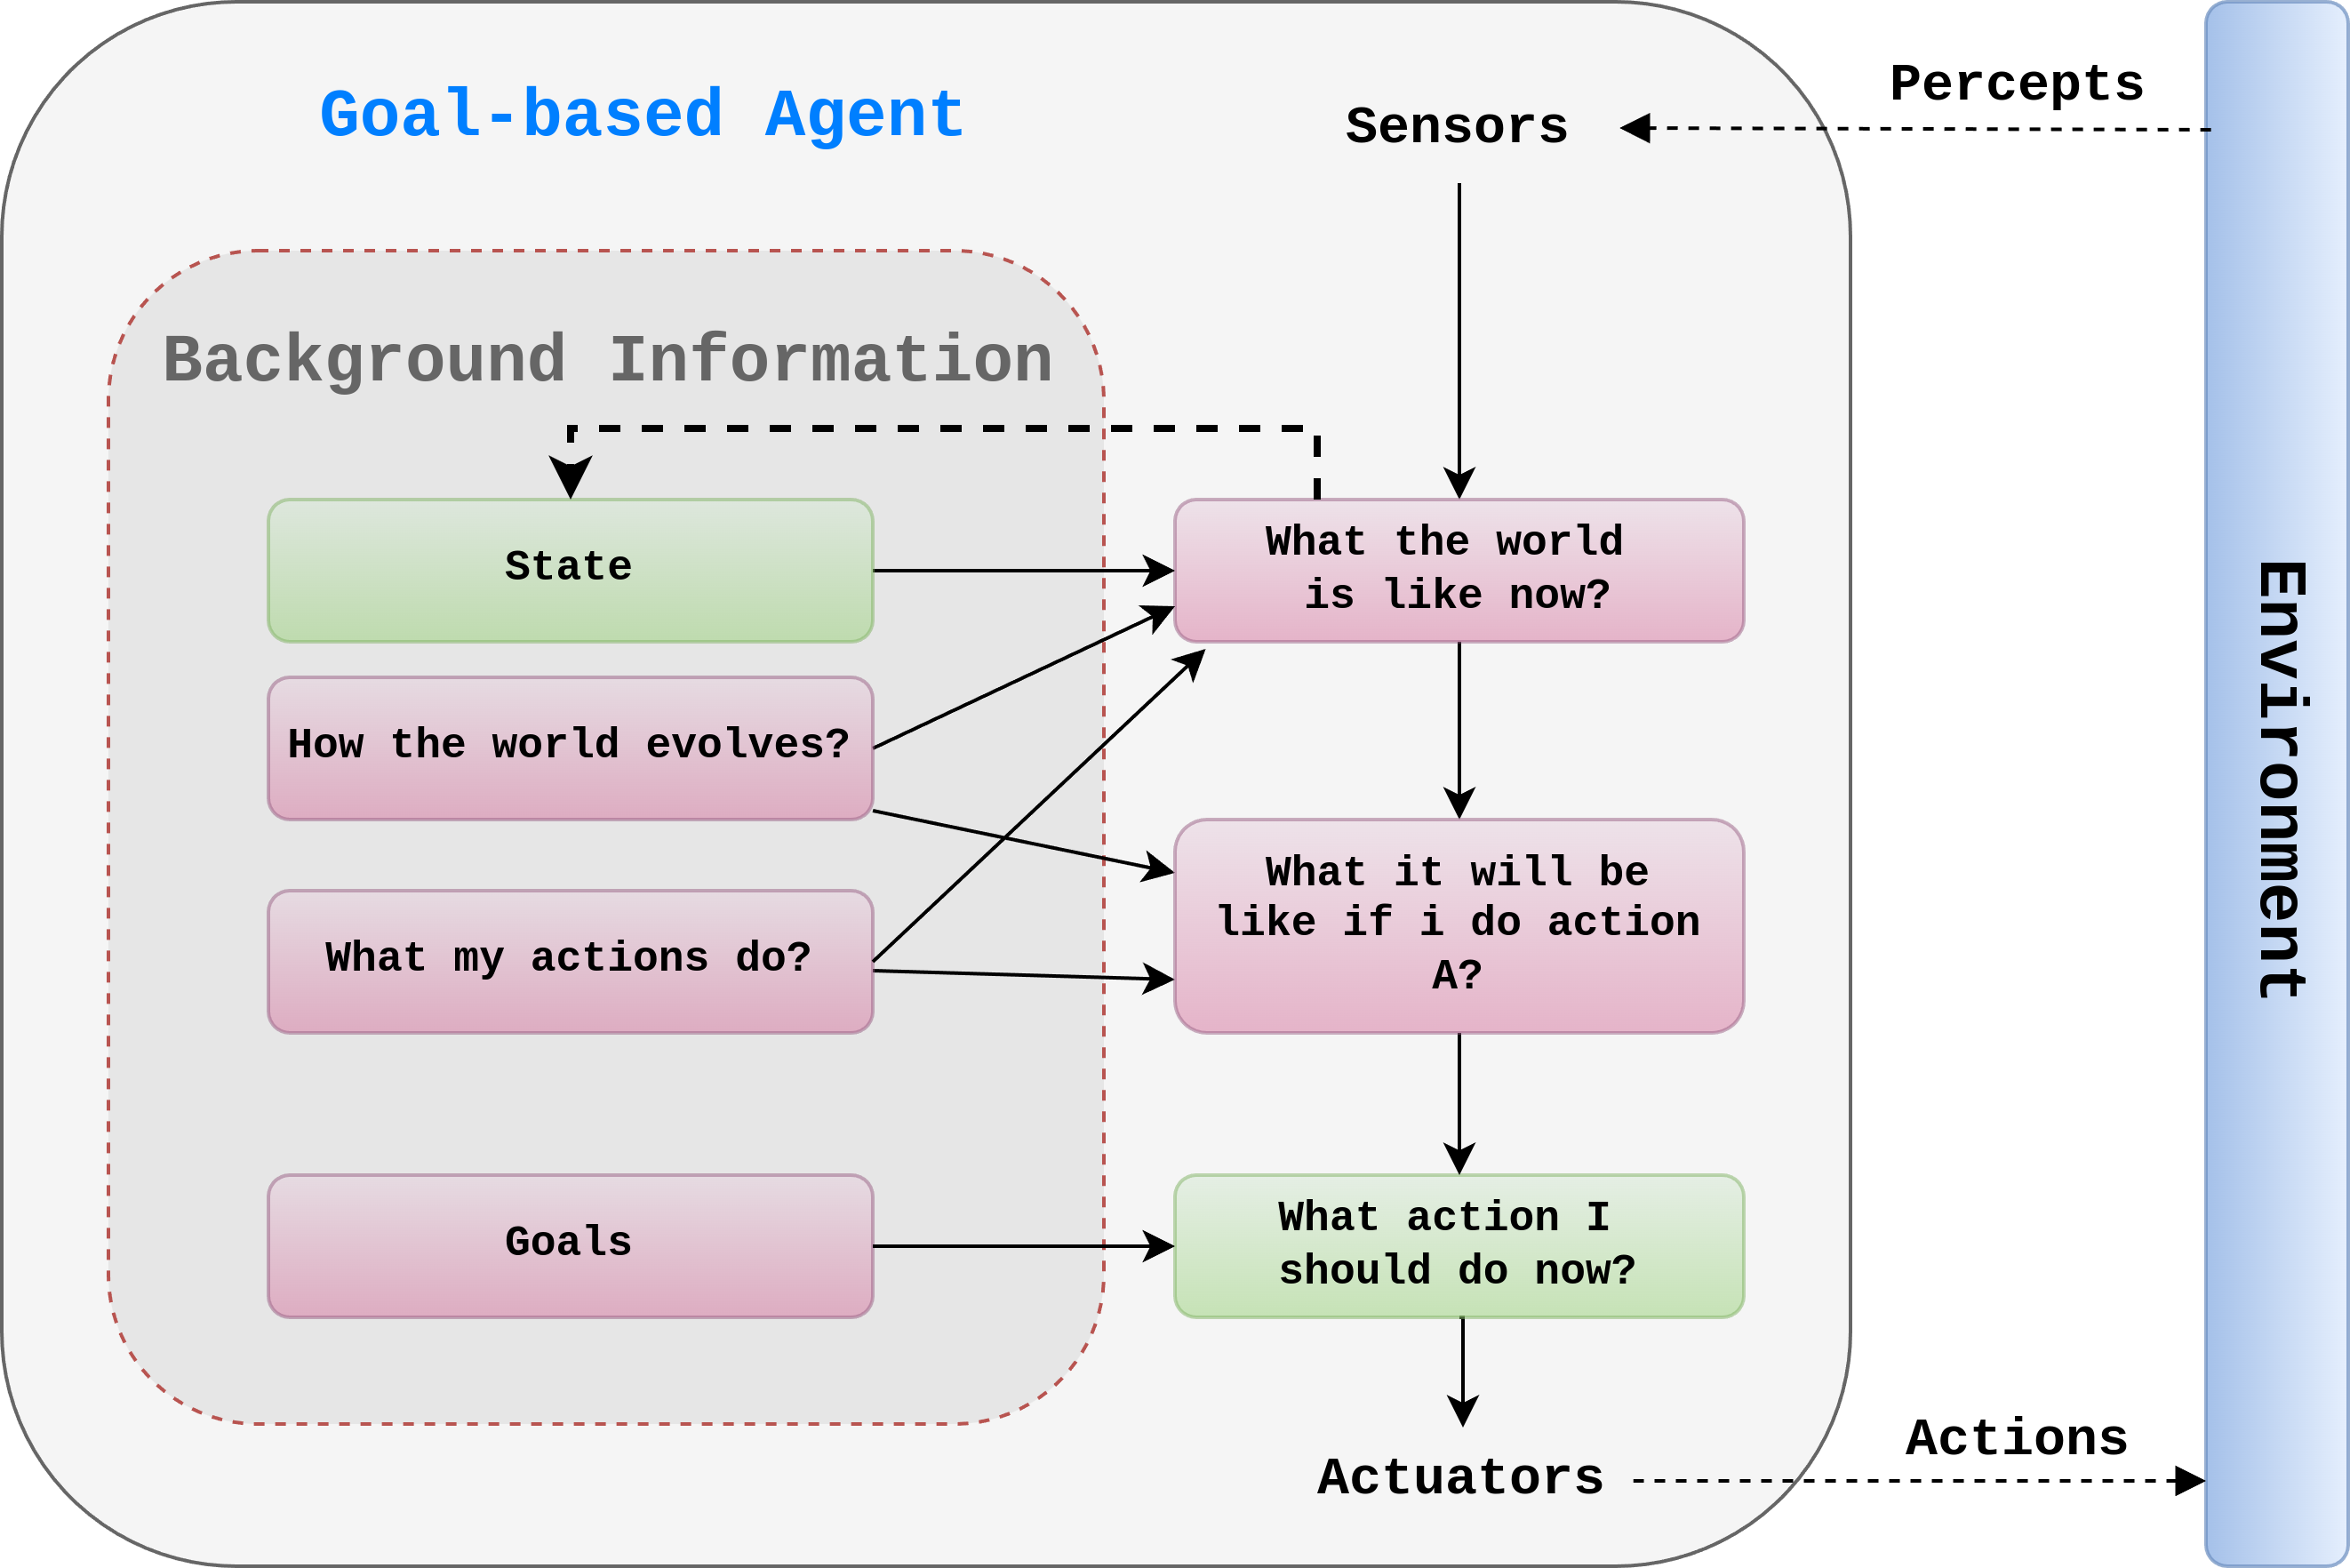
\includegraphics[
        width=0.5\linewidth, 
        height=6cm, 
        keepaspectratio
    ]{images/artificial-intelligence/ai-agents/agents-Goal-based-agent.png}
    \caption*{A model-based, goal-based agent. \cite{common/online/tools/draw.io}}
\end{figure}



\begin{enumerate}[itemsep=0.2cm]
    \item As well as a current state description, the agent needs some sort of \textbf{goal} information that describes situations that are desirable.
    \hfill \cite{ai/book/Artificial-Intelligence-A-Modern-Approach/Russell-Norvig}

    \item  The agent program can combine this with the model (the same information as was used in the modelbased reflex agent) to choose actions that achieve the goal.
    \hfill \cite{ai/book/Artificial-Intelligence-A-Modern-Approach/Russell-Norvig}

    \item Sometimes goal-based action selection is straightforward - for example, when goal satisfaction results immediately from a single action. Sometimes it will be more tricky - for example, when the agent has to consider long sequences of twists and turns in order to find a way to achieve the goal.
    \hfill \cite{ai/book/Artificial-Intelligence-A-Modern-Approach/Russell-Norvig}

    \item decision making of this kind is fundamentally different from the condition–action rules \\
    decision making involves consideration of the future - both \textit{“What will happen if I do such-and-such?”} and \textit{“Will that make me happy?”}.
    \hfill \cite{ai/book/Artificial-Intelligence-A-Modern-Approach/Russell-Norvig}

    \item It is \textbf{not reflexive}. It takes calculated decisions.

    \item Although the goal-based agent appears less efficient, it is more flexible because the knowledge that supports its decisions is represented explicitly and can be modified.
    \hfill \cite{ai/book/Artificial-Intelligence-A-Modern-Approach/Russell-Norvig}

    \item Goals just provide a crude binary distinction between “happy” and “unhappy” states.
    \hfill \cite{ai/book/Artificial-Intelligence-A-Modern-Approach/Russell-Norvig}

    \item SEE: subfields of AI devoted to finding action sequences that achieve the agent’s goals: (TODO)
    \begin{enumerate}
        \item Search
        \item Planning
    \end{enumerate}
\end{enumerate}


\section{(Model-based Goal-based) Utility-based Agents}\label{AI: Agent Programs/(Model-based Goal-based) Utility-based Agents}


\begin{figure}[H]
    \centering
    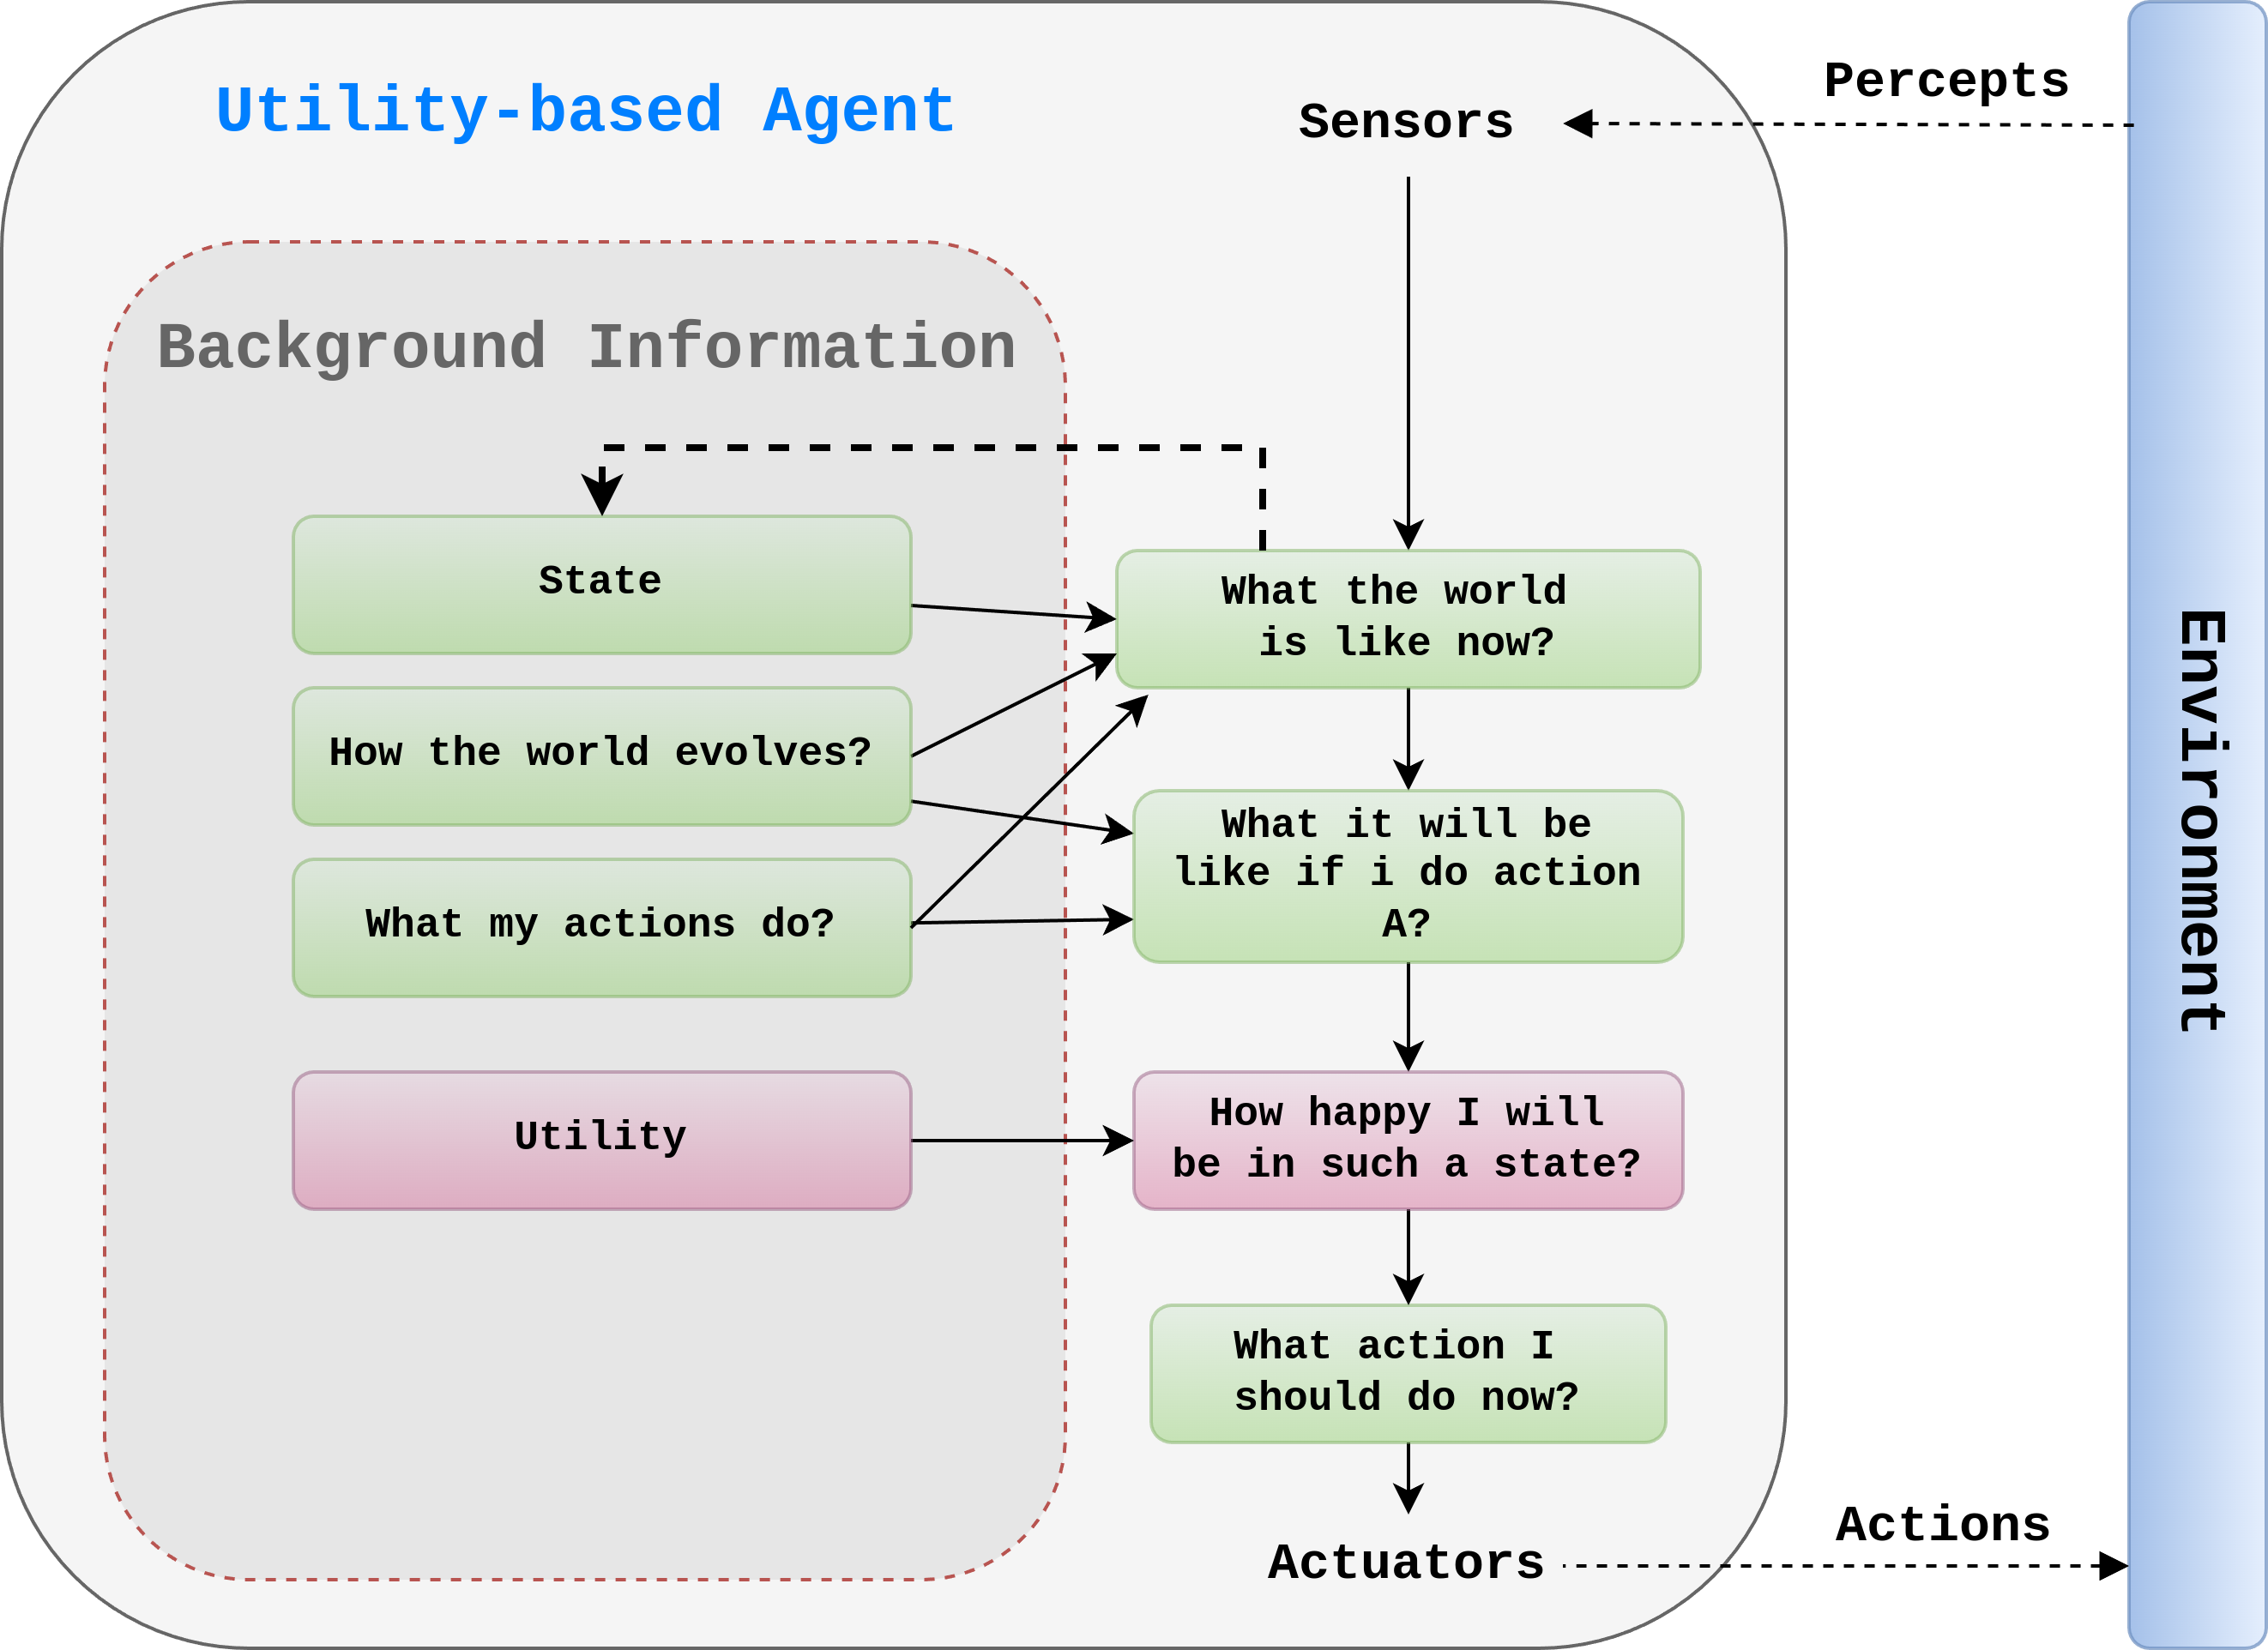
\includegraphics[
        width=0.5\linewidth,
        height=6cm,
        keepaspectratio
    ]{images/artificial-intelligence/ai-agents/agents-utility-based-agent.png}
    \caption*{A model-based, goal-based, utility-based agent. \cite{common/online/tools/draw.io}}
\end{figure}

\hspace{0.5cm}

\begin{enumerate}
    \item A more general performance measure than Goal (happy/ unhappy) should allow a comparison of different world states according to exactly how happy they would make the agent.
    \hfill \cite{ai/book/Artificial-Intelligence-A-Modern-Approach/Russell-Norvig}

    \item An agent’s \textbf{utility function} is essentially an internalization of the performance measure.
    \hfill \cite{ai/book/Artificial-Intelligence-A-Modern-Approach/Russell-Norvig}
    \\
    (The word “utility” here refers to “\textit{the quality of being useful}”)

    \item  If the internal utility function and the external performance measure are in agreement, then an agent that chooses actions to maximize its utility will be rational according to the external performance measure.
    \hfill \cite{ai/book/Artificial-Intelligence-A-Modern-Approach/Russell-Norvig}

    \item this is \textbf{not the only} way to be rational but, like goal-based agents, a utility-based agent has many advantages in terms of flexibility and learning
    \hfill \cite{ai/book/Artificial-Intelligence-A-Modern-Approach/Russell-Norvig}

    \item (\textbf{Advantage}) in two kinds of cases, goals are inadequate but a utility-based agent can still make rational decisions:
    \begin{enumerate}
        \item when there are conflicting goals, only some of which can be achieved (for example, speed and safety), the utility function specifies the appropriate tradeoff
        \hfill \cite{ai/book/Artificial-Intelligence-A-Modern-Approach/Russell-Norvig}

        \item when there are several goals that the agent can aim for, none of which can be achieved with certainty, utility provides a way in which the likelihood of success can be weighed against the importance of the goals.
        \hfill \cite{ai/book/Artificial-Intelligence-A-Modern-Approach/Russell-Norvig}
    \end{enumerate}

    \item Partial observability and stochasticity are ubiquitous in the real world, and so, therefore, is decision making under uncertainty.
    \hfill \cite{ai/book/Artificial-Intelligence-A-Modern-Approach/Russell-Norvig}

    \item a rational utility-based agent chooses the action that maximizes the expected utility of the action outcomes - that is, the utility the agent expects to derive, on average, given the probabilities and utilities of each outcome.
    \hfill \cite{ai/book/Artificial-Intelligence-A-Modern-Approach/Russell-Norvig}

    \item An agent that possesses an explicit utility function can make rational decisions with a general-purpose algorithm that does not depend on the specific utility function being maximized. In this way, the “global” definition of rationality - designating as rational those agent functions that have the highest performance - is turned into a “local” constraint on rational-agent designs that can be expressed in a simple program.
    \hfill \cite{ai/book/Artificial-Intelligence-A-Modern-Approach/Russell-Norvig}

    \item A utility-based agent has to model and keep track of its environment, tasks that have involved a great deal of research on perception, representation, reasoning, and learning.
    \hfill \cite{ai/book/Artificial-Intelligence-A-Modern-Approach/Russell-Norvig}

    \item Choosing the utility-maximizing course of action is also a difficult task, requiring ingenious algorithms.
    \hfill \cite{ai/book/Artificial-Intelligence-A-Modern-Approach/Russell-Norvig}
\end{enumerate}



\vspace{0.5cm}


\begin{customArrayStretch}{1.3}
\begin{table}[H]
\centering

\begin{tabular}{| l | l | l |}

\hline

\textbf{Aspect} &
    \textbf{Utility Function} &
    \textbf{Performance Measure} \\ \hline

\textbf{Perspective} &
    From the agent’s point of view &
    From the external evaluator’s point of view \\ \hline

\textbf{Goal} &
    Maximize expected utility &
    Maximize measurable performance \\ \hline

\textbf{Usage} &
    Guides decision-making &
    Evaluates overall system success \\ \hline

\end{tabular}

\caption*{Utility Function VS Performance Measure}
\end{table}
\end{customArrayStretch}















\section{Learning agents}\label{AI: Agent Programs/Learning agents}

\begin{figure}[H]
    \centering
    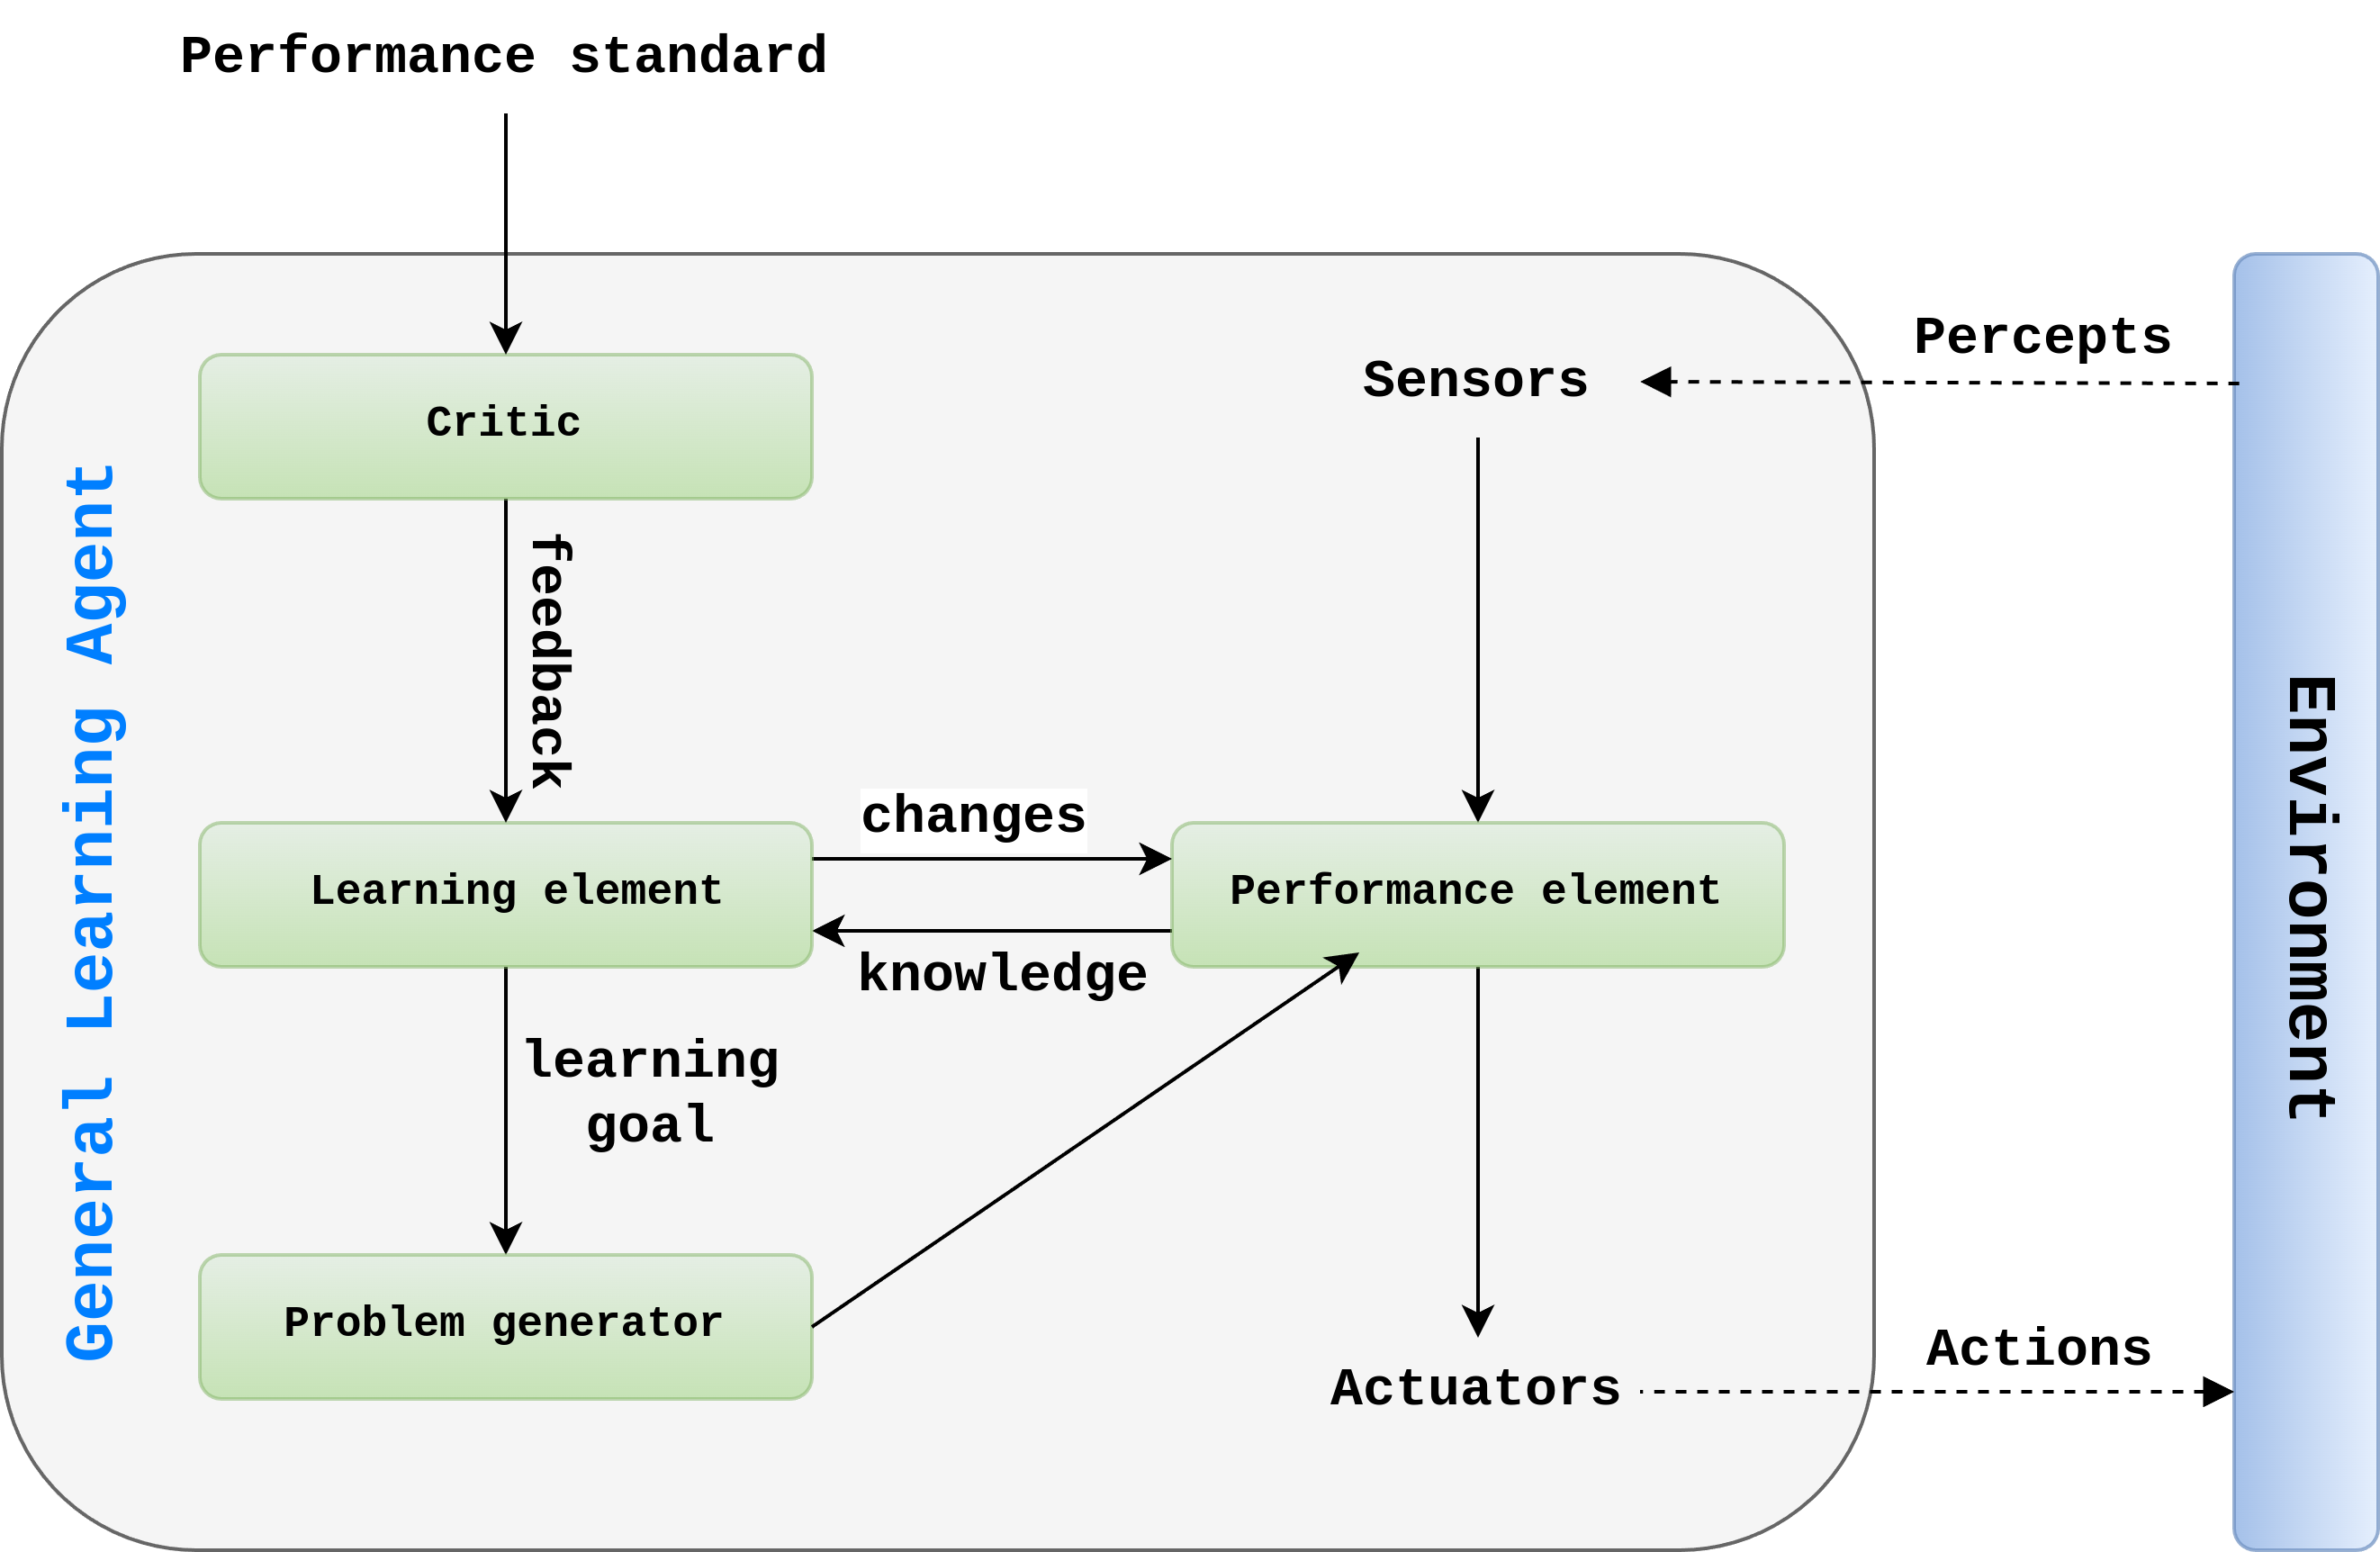
\includegraphics[
        width=0.5\linewidth, 
        height=6cm, 
        keepaspectratio
    ]{images/artificial-intelligence/ai-agents/agents-general-learning-agent.png}
    \caption*{A general learning agent. \cite{common/online/tools/draw.io}}
\end{figure}


\vspace{0.5cm}


\begin{enumerate}[itemsep=0.2cm]
    \item In his famous early paper, \textbf{Turing} (1950) considers the idea of actually programming his intelligent machines by hand.
    \hfill \cite{ai/book/Artificial-Intelligence-A-Modern-Approach/Russell-Norvig}

    \item  \textbf{advantage}: it allows the agent to operate in initially unknown environments and to become more competent than its initial knowledge alone might allow.
    \hfill \cite{ai/book/Artificial-Intelligence-A-Modern-Approach/Russell-Norvig}

    \item \textbf{conceptual components}:
    \begin{enumerate}[itemsep=0.1cm]
        \item \textbf{learning element}: responsible for making improvements
        \hfill \cite{ai/book/Artificial-Intelligence-A-Modern-Approach/Russell-Norvig}

        \item \textbf{performance element}: responsible for selecting external actions. it takes in percepts and decides on actions.
        \hfill \cite{ai/book/Artificial-Intelligence-A-Modern-Approach/Russell-Norvig}
        \\
        The design of the learning element depends very much on the design of the performance element. When trying to design an agent that learns a certain capability, the first question is \textbf{not} “\textit{How am I going to get it to learn this?}” \textbf{but} “\textit{What kind of performance element will my agent need to do this once it has learned how?}”
        \hfill \cite{ai/book/Artificial-Intelligence-A-Modern-Approach/Russell-Norvig}
        \\
        It is important that the performance standard be fixed. Conceptually, one should think of it as being outside the agent altogether because the agent \textbf{must not} modify it to fit its own behavior.
        \hfill \cite{ai/book/Artificial-Intelligence-A-Modern-Approach/Russell-Norvig}

        \item \textbf{critic}: The learning element uses feedback from the critic on how the agent is doing and determines how the performance element should be modified to do better in the future. 
        \hfill \cite{ai/book/Artificial-Intelligence-A-Modern-Approach/Russell-Norvig}
        \\
        The critic tells the learning element how well the agent is doing with respect to a fixed performance standard. The critic is necessary because the percepts themselves provide \textbf{no} indication of the agent’s success.
        \hfill \cite{ai/book/Artificial-Intelligence-A-Modern-Approach/Russell-Norvig}

        \item \textbf{problem generator}: It is responsible for suggesting actions that will lead to new and informative experiences. The point is that if the performance element had its way, it would keep doing the actions that are best, given what it knows. But if the agent is willing to explore a little and do some perhaps suboptimal actions in the short run, it might discover much better actions for the long run. 
        \hfill \cite{ai/book/Artificial-Intelligence-A-Modern-Approach/Russell-Norvig}
        \\
        The problem generator might identify certain areas of behavior in need of improvement and suggest experiments.
        \hfill \cite{ai/book/Artificial-Intelligence-A-Modern-Approach/Russell-Norvig}
         
    \end{enumerate}

    \item The learning element can make changes to any of the “\textit{knowledge}” components in the previous agents(simple reflex, model based, goal based, utility based). The simplest cases involve learning directly from the percept sequence. Observation of pairs of successive states of the environment can allow the agent to learn “How the world evolves,” and observation of the results of its actions can allow the agent to learn “What my actions do.”.
    The forms of learning do not need to access the external performance standard.
    \hfill \cite{ai/book/Artificial-Intelligence-A-Modern-Approach/Russell-Norvig}


    \item In a sense, the \textbf{external performance standard} is the \textit{universal} one of making predictions that agree with experiment.
    \hfill \cite{ai/book/Artificial-Intelligence-A-Modern-Approach/Russell-Norvig}

    \item  In a sense, the performance standard distinguishes part of the incoming percept as a \textbf{reward} (or \textbf{penalty}) that provides direct feedback on the quality of the agent’s behavior. Hard-wired performance standards such as pain and hunger in animals can be understood in this way.
    \hfill \cite{ai/book/Artificial-Intelligence-A-Modern-Approach/Russell-Norvig}

    \item Learning in intelligent agents can be summarized as a process of modification of each component of the agent to bring the components into closer agreement with the available feedback information, thereby improving the overall performance of the agent.
    \hfill \cite{ai/book/Artificial-Intelligence-A-Modern-Approach/Russell-Norvig}

    \item Intelligent agents are supposed to maximize their performance measure.
    \hfill \cite{ai/book/Artificial-Intelligence-A-Modern-Approach/Russell-Norvig}
\end{enumerate}



\section{Problem-Solving Agent}\label{AI: Agent Programs/Problem-Solving Agent}



\begin{enumerate}
    \item one kind of \textit{goal-based agent} that use \textbf{atomic} representations
    \hfill \cite{ai/book/Artificial-Intelligence-A-Modern-Approach/Russell-Norvig}

    \item \textbf{uninformed search algorithms}: algorithms that are given \textbf{no information} about the problem other than its definition
    \hfill \cite{ai/book/Artificial-Intelligence-A-Modern-Approach/Russell-Norvig}
    \\
    some of these algorithms can solve any solvable problem, none of them can do so efficiently
    \hfill \cite{ai/book/Artificial-Intelligence-A-Modern-Approach/Russell-Norvig}

    \item \textbf{Informed search algorithms}: can do quite well given some guidance on where to look for solutions.
    \hfill \cite{ai/book/Artificial-Intelligence-A-Modern-Approach/Russell-Norvig}

    \item \textbf{Goal formulation}, based on the current situation and the agent’s performance measure, is the first step in problem solving.
    \hfill \cite{ai/book/Artificial-Intelligence-A-Modern-Approach/Russell-Norvig}

    \item We consider a goal to be a set of world states—exactly those states in which the goal is satisfied.
    The agent’s task is to find out how to act, now and in the future, so that it reaches a goal state.
    \hfill \cite{ai/book/Artificial-Intelligence-A-Modern-Approach/Russell-Norvig}

\subsection*{Simple “formulate, search, execute” design}

    \item \textbf{Problem formulation} is the process of deciding what actions and states to consider, given a goal.
    \hfill \cite{ai/book/Artificial-Intelligence-A-Modern-Approach/Russell-Norvig}

    \item An agent with several immediate options of unknown value can decide what to do by first examining future actions that eventually lead to states of known value.
    \hfill \cite{ai/book/Artificial-Intelligence-A-Modern-Approach/Russell-Norvig}

    \item The process of looking for a sequence of actions that reaches the goal is called \textbf{search}.
    \hfill \cite{ai/book/Artificial-Intelligence-A-Modern-Approach/Russell-Norvig}

    \item A \textit{search algorithm} takes a problem as input and returns a \textbf{solution} in the form of an action sequence.
    \hfill \cite{ai/book/Artificial-Intelligence-A-Modern-Approach/Russell-Norvig}

    \item Once a solution is found, the actions it recommends can be carried out. This is called the \textbf{execution} phase.
    While the agent is executing the solution sequence it \textit{ignores} its percepts when choosing an action because it knows in advance what they will be.
    \hfill \cite{ai/book/Artificial-Intelligence-A-Modern-Approach/Russell-Norvig}

    \item Once the solution has been executed, the agent will formulate a new goal.
    \hfill \cite{ai/book/Artificial-Intelligence-A-Modern-Approach/Russell-Norvig}

    \item An agent that carries out its plans with its eyes closed, so to speak, must be quite certain of what is going on. Control theorists call this an \textbf{open-loop system}, because ignoring the percepts breaks the loop between agent and environment.
    \hfill \cite{ai/book/Artificial-Intelligence-A-Modern-Approach/Russell-Norvig}
\end{enumerate}








\vspace{0.5cm}


\begin{algorithm}[H]
    \caption{A simple problem-solving agent. It first formulates a goal and a problem, searches for a sequence of actions that would solve the problem, and then executes the actions one at a time. When this is complete, it formulates another goal and starts over \cite{ai/book/Artificial-Intelligence-A-Modern-Approach/Russell-Norvig}}

    \SetKwFunction{FUNCTION}{\textsc{Simple-Problem-Solving-Agent}}
    \SetKwProg{Fn}{function}{ returns \normalfont an action}{end}
    \Fn{\FUNCTION{ percept }}{
        \textbf{persistent}:\\
            \hspace{1cm} $seq$, an action sequence, initially empty \\
            \hspace{1cm} $state$, some description of the current world state \\
            \hspace{1cm} $goal$, a goal, initially null \\
            \hspace{1cm} $problem$, a problem formulation \\
        \ \\
        $state$ $\gets$ \textsc{Update-State}( $state,\ percept$ )

        \If{$seq$ \normalfont is empty}{
            $goal$ $\gets$ \textsc{Formulate-Goal}( $state$ ) \\
            $problem$ $\gets$ \textsc{Formulate-Problem}( $state,\ goal$ )\\
            $seq$ $\gets$ \textsc{Search}( $prolem$ ) \\

            \If{$seq\ = \ failure$ }{
                \Return a null action
            }
        }

        $action$ $\gets$ \textsc{First}( $seq$ )\\
        $seq$ $\gets$ \textsc{Rest}( $seq$ )

        \Return $action$
    }
\end{algorithm}



\subsection{Defining \& Formulating Problem}

\begin{enumerate}
    \item The \textbf{initial state} that the agent starts in.
    \hfill \cite{ai/book/Artificial-Intelligence-A-Modern-Approach/Russell-Norvig}

    \item A description of the possible \textbf{actions} available to the agent. Given a particular state $s$, \textsc{Actions}($s$) returns the set of actions that can be executed in $s$. We say that each of these actions is \textit{applicable} in $s$.
    \hfill \cite{ai/book/Artificial-Intelligence-A-Modern-Approach/Russell-Norvig}

    \item A description of what each action does; the formal name for this is the \textbf{transition model}, specified by a function \textsc{Result}($s,\ a$) that returns the state that results from  doing action $a$ in state $s$.
    We also use the term \textbf{successor} to refer to any state reachable from a given state by a single action.
    \hfill \cite{ai/book/Artificial-Intelligence-A-Modern-Approach/Russell-Norvig}

    \item The \textbf{goal test}, which determines whether a given state is a goal state.
    Sometimes there is an \textit{explicit} set of possible goal states, and the test simply checks whether the given state is one of them.
    Sometimes the goal is specified by an \textit{abstract property} rather than an explicitly enumerated set of states.
    \hfill \cite{ai/book/Artificial-Intelligence-A-Modern-Approach/Russell-Norvig}

    \item A \textbf{path cost} function that assigns a numeric cost to each path. The problem-solving agent chooses a cost function that reflects its own performance measure.
    We assume that the cost of a path can be described as the \textit{sum} of the costs of the individual actions along the path.
    \hfill \cite{ai/book/Artificial-Intelligence-A-Modern-Approach/Russell-Norvig}
\end{enumerate}

\vspace{0.5cm}

\textbf{Note}:

\begin{enumerate}
    \item Together, the initial state, actions, and transition model implicitly define the \textbf{state space} of the problem—the set of all states reachable from the initial state by any sequence of actions. The state space forms a directed network or \textbf{graph} in which the nodes are states and the links between nodes are actions.
    \hfill \cite{ai/book/Artificial-Intelligence-A-Modern-Approach/Russell-Norvig}

    \item \textbf{diameter of the state space}: The maximum number of steps (or actions) required to go from any one state to any other reachable state in the state space.
    \hfill \cite{ai/book/Artificial-Intelligence-A-Modern-Approach/Russell-Norvig}

    \item A \textbf{path} in the state space is a sequence of states connected by a sequence of actions.
    \hfill \cite{ai/book/Artificial-Intelligence-A-Modern-Approach/Russell-Norvig}

    \item The \textbf{step cost} of taking action $a$ in state $s$ to reach state $s^\prime$ is denoted by $c(s,\ a,\ s^\prime)$.
    \hfill \cite{ai/book/Artificial-Intelligence-A-Modern-Approach/Russell-Norvig}

    \item A \textbf{solution} to a problem is an \textit{action sequence} that leads from the initial state to a goal state.
    \hfill \cite{ai/book/Artificial-Intelligence-A-Modern-Approach/Russell-Norvig}

    \item Solution quality is measured by the path cost function, and an \textbf{optimal solution} has the lowest path cost among all solutions.
    \hfill \cite{ai/book/Artificial-Intelligence-A-Modern-Approach/Russell-Norvig}

    \item In addition to abstracting the state description, we must abstract the actions themselves.
    \hfill \cite{ai/book/Artificial-Intelligence-A-Modern-Approach/Russell-Norvig}

    \item The abstraction is \textbf{valid} if we can expand any abstract solution into a solution in the more detailed world
    \hfill \cite{ai/book/Artificial-Intelligence-A-Modern-Approach/Russell-Norvig}

    \item The abstraction is \textbf{useful} if carrying out each of the actions in the solution is easier than the original problem
    \hfill \cite{ai/book/Artificial-Intelligence-A-Modern-Approach/Russell-Norvig}

    \item \textbf{meta-level state space}: Each \textbfit{state} in a meta-level state space captures the internal (computational) state of a program that is searching in an \textbf{object-level state space}.
    Each \textbfit{action} in the meta-level state space is a computation step that alters the internal state.
    A sequence of larger and larger search trees, can be seen as depicting a path in the meta-level state space where each state on the path is an object-level search tree
    \hfill \cite{ai/book/Artificial-Intelligence-A-Modern-Approach/Russell-Norvig}
    \\
    \textbf{Example}: the internal state of the A$^\ast$ algorithm consists of the current search tree.
    each computation step in A$^\ast$ expands a leaf node and adds its successors to the tree
    \hfill \cite{ai/book/Artificial-Intelligence-A-Modern-Approach/Russell-Norvig}

    \item \textbf{meta-level learning algorithm} can learn from experiences (missteps in harder problems) to avoid exploring unpromising sub-trees.
    The goal of learning is to \textit{minimize} the \textbf{total cost} of problem solving, trading off computational expense and path cost.
    \hfill \cite{ai/book/Artificial-Intelligence-A-Modern-Approach/Russell-Norvig}

    \item \textbf{relaxed problem}: A problem with \textit{fewer restrictions} on the actions
    \hfill \cite{ai/book/Artificial-Intelligence-A-Modern-Approach/Russell-Norvig}
    \\
    The state-space graph of the relaxed problem is a \textbf{super-graph} of the original state space because the removal of restrictions creates added edges in the graph.
    \hfill \cite{ai/book/Artificial-Intelligence-A-Modern-Approach/Russell-Norvig}
    \\
    Because the relaxed problem adds edges to the state space, any optimal solution in the original problem is, by definition, also a solution in the relaxed problem; but the relaxed problem may have \textbf{better solutions} if the added edges provide \textbf{short cuts}. Hence, \textbfit{the cost of an optimal solution to a relaxed problem is an admissible heuristic for the original problem}.
    \hfill \cite{ai/book/Artificial-Intelligence-A-Modern-Approach/Russell-Norvig}
    \\
    because the derived heuristic is an exact cost for the relaxed problem, it must obey the triangle inequality and is therefore \textbf{consistent}
    \hfill \cite{ai/book/Artificial-Intelligence-A-Modern-Approach/Russell-Norvig}

    \item  it is crucial that the relaxed problems generated by this technique can be solved essentially \textbf{without search}, because the relaxed rules allow the problem to be decomposed into some independent subproblems.
    If the relaxed problem is hard to solve, then the values of the corresponding heuristic will be \textbf{expensive} to obtain.
    \hfill \cite{ai/book/Artificial-Intelligence-A-Modern-Approach/Russell-Norvig}
\end{enumerate}

\vspace{0.2cm}

\begin{lstlisting}[
    language=Python,
    caption=Problem Solving Agent - Problem Skeleton
]
class Problem:
    def __init__(self, initial_state: State):
        self.initial_state = initial_state
        # 1. initial_state: The initial state that the agent starts in.

    def actions(self, state: State):
        """
            2. A description of the possible actions available to the agent.
            Given a particular state s, ACTIONS(s) returns the set of actions
            that can be executed in s.
        """
        raise NotImplementedError()

    def result(self, state: State, action):
        """
            3. A description of what each action does; the formal name for this
            is the transition model, specified by a function RESULT(s, a) that
            returns the state that results from doing action a in state s.
        """
        raise NotImplementedError()

    def goal_test(self, state: State):
        # 4. The goal test, which determines whether a given state is a goal state.
        raise NotImplementedError()

    def step_cost(self, state: State, action, new_state: State):
        """
            5. The step cost of taking action
            a in state s to reach state s' is denoted by c(s, a, s').
        """
        raise NotImplementedError()

    def heuristic(self, state: State):
        """
            Returns estimated cost from state to goal.
        """
        raise NotImplementedError()
\end{lstlisting}



\subsection{Measuring problem-solving performance}

\begin{enumerate}
    \item \textbf{Completeness}: Is the algorithm guaranteed to find a solution when there is one?
    \hfill \cite{ai/book/Artificial-Intelligence-A-Modern-Approach/Russell-Norvig}

    \item \textbf{Optimality}: Does the strategy find the optimal solution?
    \hfill \cite{ai/book/Artificial-Intelligence-A-Modern-Approach/Russell-Norvig}

    \item \textbf{Time complexity}: How long does it take to find a solution?
    \hfill \cite{ai/book/Artificial-Intelligence-A-Modern-Approach/Russell-Norvig}

    \item \textbf{Space complexity}: How much memory is needed to perform the search?
    \hfill \cite{ai/book/Artificial-Intelligence-A-Modern-Approach/Russell-Norvig}
\end{enumerate}


\vspace{0.5cm}

\begin{customArrayStretch}{1.3}
\begin{table}[H]
\centering
\begin{tabular}{l l p{12cm}}

$V$ & set & set of vertices (nodes) of the graph \\

$E$ & set & set of edges (links) of the graph \\

$b$ & $\in \mbbR$ & \textbf{branching factor} or maximum number of successors of any node \\

$d$ & $\in \mbbR$ & \textbf{depth} of the \textbf{shallowest goal} node (i.e., the number of steps along the path from the root) \\

$m$ & $\in \mbbR$ & maximum length of any path in the state space \\

\end{tabular}
\caption*{Notations}
\end{table}
\end{customArrayStretch}


\textbf{Note}:
\begin{enumerate}
    \item the typical measure is the \textbf{size} of the \textbf{state space graph}: $|V| + |E|$
    \hfill \cite{ai/book/Artificial-Intelligence-A-Modern-Approach/Russell-Norvig}

    \item Time is often measured in terms of the number of nodes generated during the search, and space in terms of the maximum number of nodes stored in memory.
    \hfill \cite{ai/book/Artificial-Intelligence-A-Modern-Approach/Russell-Norvig}

    \item \textbf{effectiveness of a search algorithm}:
    \begin{enumerate}
        \item \textbf{search cost}: depends on the time complexity but can also include a term for memory usage
        \hfill \cite{ai/book/Artificial-Intelligence-A-Modern-Approach/Russell-Norvig}

        \item \textbf{total cost}: combines the search cost and the path cost of the solution found
        \hfill \cite{ai/book/Artificial-Intelligence-A-Modern-Approach/Russell-Norvig}
    \end{enumerate}

    \item In general, exponential-complexity search problems \textbf{cannot be solved} by uninformed methods for any but the smallest instances.
\end{enumerate}







\section{Planning Agents}\label{AI: Agent Programs/Planning Agents}


\begin{enumerate}[itemsep=0.2cm]
    \item One kind of \textit{goal-based agents} that use more advanced \textbf{factored} or \textbf{structured} representations
    \hfill \cite{ai/book/Artificial-Intelligence-A-Modern-Approach/Russell-Norvig}



\end{enumerate}

















\section{Examples}
\subsection{Vacuum Cleaner \cite{ai/book/Artificial-Intelligence-A-Modern-Approach/Russell-Norvig}}


\begin{figure}[H]
    \centering
    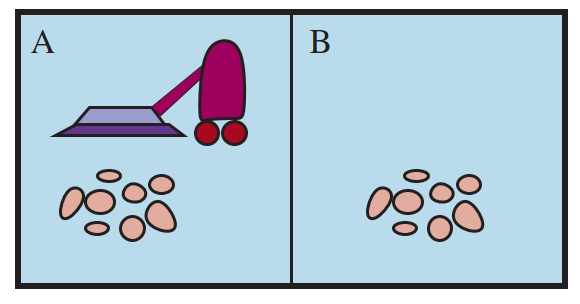
\includegraphics[
        width=0.5\linewidth
    ]{images/artificial-intelligence/examples/example-vacuum-cleaner-world.png}
    \caption*{A vacuum-cleaner world with just two locations}
\end{figure}


\vspace{0.5cm}

\begin{enumerate}[itemsep=0.2cm]
    \item it’s a made-up world

    \item This particular world has just two locations: squares A and B. 
    
    \item The vacuum agent perceives which square it is in and whether there is dirt in the square. 
    
    \item It can choose to \textbf{move left}, \textbf{move right}, \textbf{suck up the dirt}, or \textbf{do nothing}.

    \item One very simple agent function is the following: if the current square is dirty, then suck; otherwise, move to the other square.

    
\end{enumerate}



\subsubsection{As a table driven agent}

\begin{customArrayStretch}{1.3}
\begin{longtable}{|l|l|}

\hline
\textbf{Percept sequence} & \textbf{Action} \\ \hline
\endhead

\hline
\textbf{Percept sequence} & \textbf{Action} \\ \hline
\endfirsthead

\hline\endfoot
\hline\endlastfoot


$[A, \ Clean]$ & $Right$ \\ 
$[A, \ Dirty]$ & $Suck$ \\ 
$[B, \ Clean]$ & $Left$ \\ 
$[B, \ Dirty]$ & $Suck$ \\ 

\vdots & \vdots \\

$[A, \ Clean],\ [A, \ Clean]$ & $Right$ \\ 
$[A, \ Clean],\ [A, \ Dirty]$ & $Suck$ \\ 

\vdots & \vdots \\

$[A, \ Clean],\ [A, \ Clean],\ [A, \ Clean]$ & $Right$ \\ 
$[A, \ Clean],\ [A, \ Clean],\ [A, \ Dirty]$ & $Suck$ \\ 

\vdots & \vdots \\

\end{longtable}
\end{customArrayStretch}





\subsubsection{As a simple reflex agent}

\begin{algorithm}[H]
    \caption{The agent program for a simple reflex agent in the two-state vacuum environment.  \cite{ai/book/Artificial-Intelligence-A-Modern-Approach/Russell-Norvig}}

    \SetKwFunction{FUNCTION}{\textsc{Reflex-Vacuum-Agent}}
    \SetKwProg{Fn}{function}{ returns \normalfont{an action}}{end}
    \Fn{\FUNCTION{[location, status]}}{
        \textbf{if} $status \ = \ Dirty$ \textbf{then return} $Suck$ \\

        \textbf{else if} $location \ = \ A$ \textbf{then return} $Right$ \\

        \textbf{else if} $location \ = \ B$ \textbf{then return} $Left$ \\
    }
\end{algorithm}
















\subsection{Automated Taxi Driver \cite{ai/book/Artificial-Intelligence-A-Modern-Approach/Russell-Norvig}}

\begin{enumerate}[itemsep=0.2cm]
    \item \textbf{Performance Measure}: Safe, fast, legal, comfortable trip, maximize profits
    \hfill \cite{ai/book/Artificial-Intelligence-A-Modern-Approach/Russell-Norvig}

    \item \textbf{Environment}: Roads, other traffic, pedestrians, customers
    \hfill \cite{ai/book/Artificial-Intelligence-A-Modern-Approach/Russell-Norvig}

    \item \textbf{Actuators}: Steering, accelerator, brake, signal, horn, display
    \hfill \cite{ai/book/Artificial-Intelligence-A-Modern-Approach/Russell-Norvig}

    \item \textbf{Sensors}: Cameras, sonar, speedometer, GPS, odometer, accelerometer, engine sensors, keyboard
    \hfill \cite{ai/book/Artificial-Intelligence-A-Modern-Approach/Russell-Norvig}

    \item an automated taxi cannot see what other drivers are thinking.
    \hfill \cite{ai/book/Artificial-Intelligence-A-Modern-Approach/Russell-Norvig}

    \item partially cooperative multiagent environment: avoiding collisions maximizes the performance measure of all agents
    \hfill \cite{ai/book/Artificial-Intelligence-A-Modern-Approach/Russell-Norvig}

    \item \textbf{Task Environment}: partially observable, multiagent, stochastic, sequential, dynamic, continuous, and unknown
    \hfill \cite{ai/book/Artificial-Intelligence-A-Modern-Approach/Russell-Norvig}
    
\end{enumerate}



\subsubsection{As a table driven reflex agent}

\begin{enumerate}[itemsep=0.2cm]
    \item the visual input from a single camera comes in at the rate of roughly $27$ megabytes per second ($30$ frames per second, $640 \times 480$ pixels with $24$-bits of color information). 
    \hfill \cite{ai/book/Artificial-Intelligence-A-Modern-Approach/Russell-Norvig}
    
    \item This gives a lookup table with over $10^{250,000,000,000}$ entries for \textbf{an hour}’s driving.
    \hfill \cite{ai/book/Artificial-Intelligence-A-Modern-Approach/Russell-Norvig}

    \item \textbf{Not possible} to construct the table
    \hfill \cite{ai/book/Artificial-Intelligence-A-Modern-Approach/Russell-Norvig}
\end{enumerate}



\subsubsection{As model-based reflex agents}

\begin{enumerate}[itemsep=0.2cm]
    \item the taxi may be driving back home, and it may have a rule telling it to fill up with gas on the way home unless it has at least half a tank. 
    \hfill \cite{ai/book/Artificial-Intelligence-A-Modern-Approach/Russell-Norvig}
    
    \item Although “driving back home” may seem to an aspect of the world state, the fact of the taxi’s destination is actually an aspect of the agent’s internal state. 
    \hfill \cite{ai/book/Artificial-Intelligence-A-Modern-Approach/Russell-Norvig}
    
    \item If you find this puzzling, consider that the taxi could be in exactly the same place at the same time, but intending to reach a different destination.
    \hfill \cite{ai/book/Artificial-Intelligence-A-Modern-Approach/Russell-Norvig}
    
\end{enumerate}


\subsubsection{As utility-based agents}

\begin{enumerate}[itemsep=0.2cm]
    \item \textbf{utility measures}: quicker, safer, more reliable, or cheaper 
    \hfill \cite{ai/book/Artificial-Intelligence-A-Modern-Approach/Russell-Norvig}
\end{enumerate}


\subsubsection{As Learning Agent}

\begin{enumerate}[itemsep=0.2cm]
    \item The performance element consists of whatever collection of knowledge and procedures the taxi has for selecting its driving actions.
    \hfill \cite{ai/book/Artificial-Intelligence-A-Modern-Approach/Russell-Norvig}

    \item  after the taxi makes a quick left turn across three lanes of traffic, the critic observes the shocking language used by other drivers.
    \hfill \cite{ai/book/Artificial-Intelligence-A-Modern-Approach/Russell-Norvig}

    \item From this experience, the learning element is able to formulate a rule saying this was a bad action, and the performance element is modified by installation of the new rule. 
    \hfill \cite{ai/book/Artificial-Intelligence-A-Modern-Approach/Russell-Norvig}

    
\end{enumerate}










\subsection{Road trip in Romania \cite{ai/book/Artificial-Intelligence-A-Modern-Approach/Russell-Norvig}}


\begin{figure}[H]
    \centering
    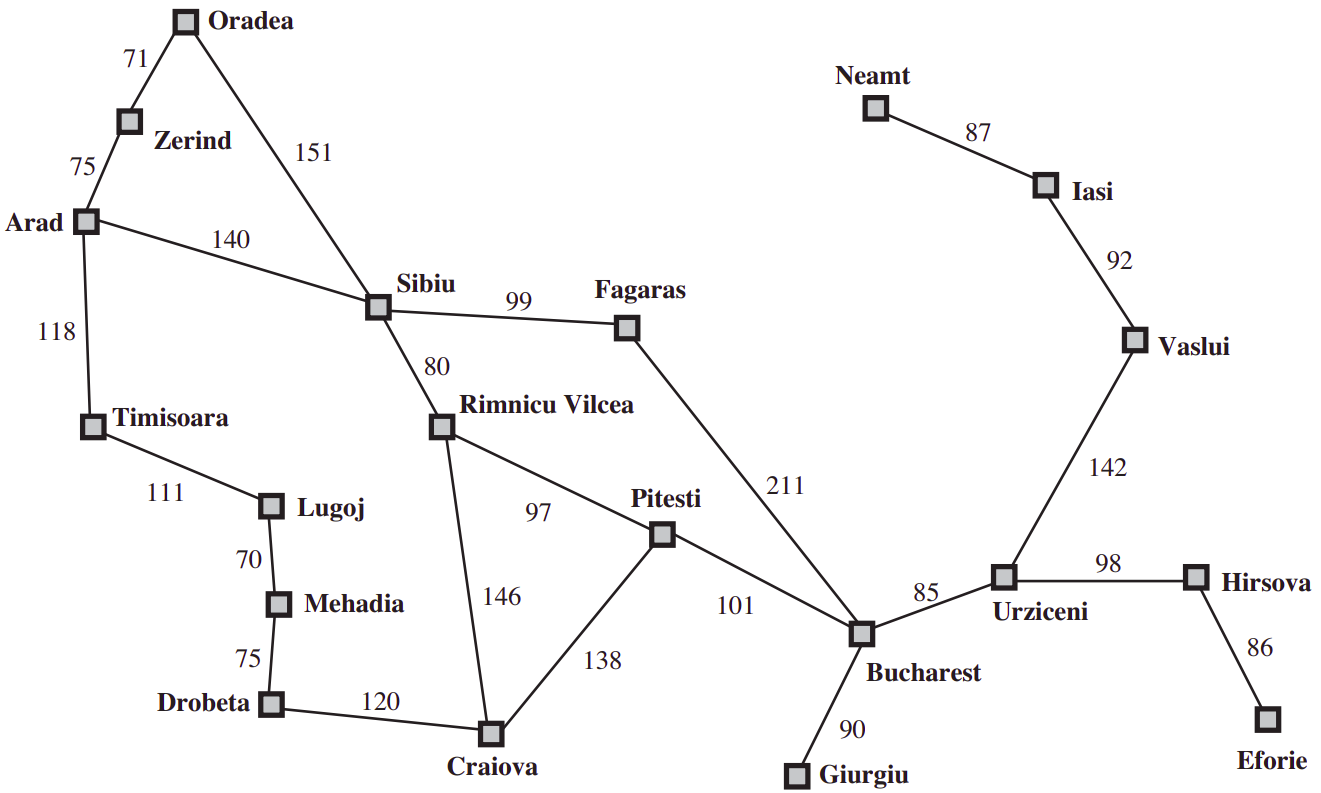
\includegraphics[
        width=\linewidth,
        height=6cm,
        keepaspectratio,
    ]{images/artificial-intelligence/examples/example-romania.png}
    \caption*{A simplified road map of part of Romania. \cite{ai/book/Artificial-Intelligence-A-Modern-Approach/Russell-Norvig}}
\end{figure}



































\chapter{AI: Searching Solutions}


\begin{enumerate}
    \item A solution is an action sequence, so search algorithms work by considering various possible action sequences.
    \hfill \cite{ai/book/Artificial-Intelligence-A-Modern-Approach/Russell-Norvig}

    \item The possible action sequences starting at the initial state form a \textbf{search tree} with the initial state at the root; the branches are actions and the \textbf{nodes} correspond to states in the state space of the problem.
    \hfill \cite{ai/book/Artificial-Intelligence-A-Modern-Approach/Russell-Norvig}

    \item We consider taking various actions by \textbf{expanding} the current state; that is, applying each legal action to the current state, thereby \textbf{generating} a new set of states.
    The process of expanding nodes on the frontier continues until either a solution is found or there are no more states to expand.
    \hfill \cite{ai/book/Artificial-Intelligence-A-Modern-Approach/Russell-Norvig}

    \item \textbf{leaf node}: a node with \textbf{no} children in the tree.
    \hfill \cite{ai/book/Artificial-Intelligence-A-Modern-Approach/Russell-Norvig}

    \item \textbf{frontier/ open list}: set of all leaf nodes available for expansion at any given point
    \hfill \cite{ai/book/Artificial-Intelligence-A-Modern-Approach/Russell-Norvig}

    \item Search algorithms all share this basic structure; they vary primarily according to how they choose which state to expand next - the so-called \textbf{search strategy}.
    \hfill \cite{ai/book/Artificial-Intelligence-A-Modern-Approach/Russell-Norvig}

    \item Considering \textbf{loopy paths} means that the complete search tree is \textbf{infinite} because there is no limit to how often one can traverse a loop.
    loops can cause certain algorithms to fail, making otherwise solvable problems \textbf{unsolvable}.
    \hfill \cite{ai/book/Artificial-Intelligence-A-Modern-Approach/Russell-Norvig}

    \item In some cases, \textbf{redundant paths} are \textit{unavoidable}. This includes all problems where the actions are reversible, such as route-finding problems and sliding-block puzzles.
    Following redundant paths can cause a tractable problem to become \textbf{intractable}. This is true even for algorithms that know how to avoid infinite loops.
    \hfill \cite{ai/book/Artificial-Intelligence-A-Modern-Approach/Russell-Norvig}
\end{enumerate}



\section{Designing Search Node}

\begin{figure}[H]
    \centering
    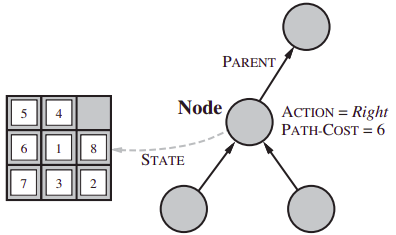
\includegraphics[
        width=0.5\linewidth,
        height=4cm,
        keepaspectratio,
    ]{images/artificial-intelligence/searching/search-node-sample.png}
    \caption*{Nodes are the data structures from which the search tree is constructed. Each has a parent, a state, and various bookkeeping fields. Arrows point from child to parent. \cite{ai/book/Artificial-Intelligence-A-Modern-Approach/Russell-Norvig}}
\end{figure}


\noindent
For each \textsc{Node} $n$ of the tree, we have a structure that contains four components:
\begin{enumerate}
    \item $n$.\textsc{State}: the state in the state space to which the node corresponds
    \hfill \cite{ai/book/Artificial-Intelligence-A-Modern-Approach/Russell-Norvig}

    \item $n$.\textsc{Parent}: the node in the search tree that generated this node
    \hfill \cite{ai/book/Artificial-Intelligence-A-Modern-Approach/Russell-Norvig}

    \item $n$.\textsc{Action}: the action that was applied to the parent to generate the node
    \hfill \cite{ai/book/Artificial-Intelligence-A-Modern-Approach/Russell-Norvig}

    \item $n$.\textsc{Path-Cost}: the cost, traditionally denoted by $g(n)$, of the path from the initial state to the node, as indicated by the parent pointers
    \hfill \cite{ai/book/Artificial-Intelligence-A-Modern-Approach/Russell-Norvig}
\end{enumerate}


\vspace{0.3cm}


\textbf{Note}:
\begin{enumerate}
    \item A node is a bookkeeping data structure used to represent the search tree.
    A state corresponds to a configuration of the world.
    Thus, nodes are on particular paths, as defined by \textsc{Parent} pointers, whereas states are not.
    Furthermore, two different nodes can contain the same world state if that state is generated via two different search paths.
    \hfill \cite{ai/book/Artificial-Intelligence-A-Modern-Approach/Russell-Norvig}

    \item The \textsc{Parent} pointers string the nodes together into a tree structure. These pointers also allow the solution path to be extracted when a goal node is found.
    \hfill \cite{ai/book/Artificial-Intelligence-A-Modern-Approach/Russell-Norvig}

    \item \textsc{Solution} function is used to return the sequence of actions obtained by following parent pointers back to the root.
    \hfill \cite{ai/book/Artificial-Intelligence-A-Modern-Approach/Russell-Norvig}
\end{enumerate}

\vspace{0.5cm}

\begin{lstlisting}[
    language=Python,
    caption=Problem Solving Agent - Search Node
]
class Node:
    def __init__(self, state, parent, action, path_cost):
        # the state in the state space to which the node corresponds
        self.state = state

        # the node in the search tree that generated this node
        self.parent = parent

        # the action that was applied to the parent to generate the node
        self.action = action

        """
            the cost, traditionally denoted by g(n), of the path
            from the initial state to the node, as indicated
            by the parent pointers
        """
        self.path_cost = path_cost

    def __lt__(self, __o):
        return self.path_cost < __o.path_cost

    def __str__(self):
        return (
            "<Node "
            + f"state: {self.state} "
            + f"parent: {self.parent} "
            + f"action: {self.action} "
            + f"path_cost: {self.path_cost} "
            + ">"
        )

    def __repr__(self) -> str:
        return str(self)
\end{lstlisting}



\begin{lstlisting}[
    language=Python,
    caption=Problem Solving Agent - solution
]
def solution(node: Node):
    path = []

    while node.parent is not None:
        path.insert(0, node.action)
        node = node.parent

    return path
\end{lstlisting}






\section{General Algorithms \& Implementations}

\subsection{Child-node}

\vspace{0.2cm}

\begin{algorithm}[H]
    \caption{The function \textsc{Child-Node} takes a parent node and an action and returns the resulting child node \cite{ai/book/Artificial-Intelligence-A-Modern-Approach/Russell-Norvig}}

    \SetKwFunction{FUNCTION}{\textsc{Child-Node}}
    \SetKwProg{Fn}{function}{ returns \normalfont{a \textsc{Node}}}{end}
    \Fn{\FUNCTION{problem}}{
        \Return a node with\\
            \hspace{1cm} \textsc{State} = $problem$.\textsc{Result}($parent$.\textsc{State}, $action$),\\
            \hspace{1cm} \textsc{Parent} = $parent$,\\
            \hspace{1cm} \textsc{Action} = $action$, \\
            \hspace{1cm} \textsc{Path-Cost} = $parent$.\textsc{Path-Cost} +
                $problem$.\textsc{Step-Cost}($parent$.\textsc{State}, $action$)
    }
\end{algorithm}


\begin{lstlisting}[
    language=Python,
    caption=Problem Solving Agents - child\_node
]
def child_node(problem: Problem, parent: Node, action):
    new_state = problem.result(parent.state, action)

    return Node(
        state=new_state,
        parent=parent,
        action=action,
        path_cost=(parent.path_cost
            + problem.step_cost(parent.state, action, new_state))
    )
\end{lstlisting}



\subsection{Tree Search}
\vspace{0.2cm}

\begin{algorithm}[H]
    \caption{An informal description of the general tree-search algorithm. \cite{ai/book/Artificial-Intelligence-A-Modern-Approach/Russell-Norvig}}

    \SetKwFunction{FUNCTION}{\textsc{Tree-Search}}
    \SetKwProg{Fn}{function}{ returns \normalfont{a solution, or failure}}{end}
    \Fn{\FUNCTION{problem}}{
        initialize the frontier using the initial state of problem\\
        \ \\
        \While{}{
            \If{the frontier is empty}{
                \Return failure
            }
            choose a leaf node and remove it from the frontier\\
            \If{the node contains a goal state}{
                \Return the corresponding solution
            }
            expand the chosen node, adding the resulting nodes to the frontier
        }
    }
\end{algorithm}


\begin{lstlisting}[
    language=Python,
    caption=Problem Solving Agents - tree\_search
]
def tree_search(problem: Problem):
    frontier = [Node(problem.initial_state, None, None, 0)]

    while True:
        if len(frontier) == 0:
            return None

        node: Node = frontier.pop()

        if problem.goal_test(node.state):
            return solution(node)

        for action in problem.actions(node.state):
            new_state = problem.result(node.state, action)
            path_cost = (node.path_cost
                + problem.step_cost(node.state, action, new_state))
            new_node = Node(new_state, node, action, path_cost)
            frontier.append(new_node)
\end{lstlisting}




\subsection{Graph search}
\vspace{0.2cm}

\begin{algorithm}[H]
    \caption{An informal description of the general graph-search algorithm. The parts of \textsc{Graph-Search} marked in bold italic are the additions needed to handle repeated states. \cite{ai/book/Artificial-Intelligence-A-Modern-Approach/Russell-Norvig}}

    \SetKwFunction{FUNCTION}{\textsc{Graph-Search}}
    \SetKwProg{Fn}{function}{ returns \normalfont{a solution, or failure}}{end}
    \Fn{\FUNCTION{problem}}{
        initialize the frontier using the initial state of problem \\
        \textbfit{initialize the explored set to be empty} \\
        \ \\
        \While{}{
            \If{the frontier is empty}{
                \Return failure
            }
            choose a leaf node and remove it from the frontier\\
            \If{the node contains a goal state}{
                \Return the corresponding solution
            }
            \textbfit{add the node to the explored set} \\
            \If{\bfseries chosen node not in the frontier or explored set}{
                expand the chosen node, adding the resulting nodes to the frontier
            }
        }
    }
\end{algorithm}

\begin{lstlisting}[
    language=Python,
    caption=Problem Solving Agents - graph\_search
]
def graph_search(problem: Problem):
    frontier = [Node(problem.initial_state, None, None, 0)]
    explored = set()

    while True:
        if len(frontier) == 0:
            return None

        node: Node = frontier.pop()

        if problem.goal_test(node.state):
            return solution(node)

        explored.add(node)

        for action in problem.actions(node.state):
            new_state = problem.result(node.state, action)
            path_cost = (node.path_cost
                + problem.step_cost(node.state, action, new_state))
            new_node = Node(new_state, node, action, path_cost)

            if new_node not in frontier and new_node not in explored:
                frontier.append(new_node)
\end{lstlisting}


\begin{enumerate}
    \item \textbf{explored set/ closed list}: remembers every expanded node
    \hfill \cite{ai/book/Artificial-Intelligence-A-Modern-Approach/Russell-Norvig}

    \item Newly generated nodes that match previously generated nodes - ones in the explored set or the frontier - can be discarded instead of being added to the frontier.
    \hfill \cite{ai/book/Artificial-Intelligence-A-Modern-Approach/Russell-Norvig}

    \item the search tree constructed by the \textsc{Graph-Search} algorithm contains \textbf{at most one copy} of each state, so we can think of it as growing a tree directly on the state-space graph.
    \hfill \cite{ai/book/Artificial-Intelligence-A-Modern-Approach/Russell-Norvig}

    \item The explored set can be implemented with a \textbf{hash table} to allow efficient checking for repeated states.
    \hfill \cite{ai/book/Artificial-Intelligence-A-Modern-Approach/Russell-Norvig}


\end{enumerate}



\section{Search Strategies/ Search Algorithms}

\subsection{Uninformed Search/ Blind Search}

\begin{enumerate}
    \item strategies have \textbf{no} additional information about states beyond that provided in the problem definition.
    \hfill \cite{ai/book/Artificial-Intelligence-A-Modern-Approach/Russell-Norvig}

    \item All they can do is generate successors and distinguish a goal state from a non-goal state. All search strategies are distinguished by the order in which nodes are expanded.
    \hfill \cite{ai/book/Artificial-Intelligence-A-Modern-Approach/Russell-Norvig}
\end{enumerate}


\vspace{0.3cm}
\textbf{SEE}:
\begin{enumerate}
    \item[] \fullref{AI: Algorithms/Breadth-first search (BFS)}
    \item[] \fullref{AI: Algorithms/Uniform-cost search (UCS)}
    \item[] \fullref{AI: Algorithms/Depth-first search (DFS)}
    \item[] \fullref{AI: Algorithms/Backtracking Search}
    \item[] \fullref{AI: Algorithms/Depth-limited search (DLS)}
    \item[] \fullref{AI: Algorithms/Iterative Deepening Search (IDS)}
    \item[] \fullref{AI: Algorithms/Iterative Lengthening Search (ILS)}
    \item[] \fullref{AI: Algorithms/Bidirectional search}
\end{enumerate}




\subsection{Informed Search/ Heuristic Search}

\begin{enumerate}
    \item Strategies that know whether one non-goal state is “\textit{more promising}” than another
    \hfill \cite{ai/book/Artificial-Intelligence-A-Modern-Approach/Russell-Norvig}

    \item uses problem-specific knowledge beyond the definition of the problem itself - can find solutions more efficiently than can an uninformed strategy.
    \hfill \cite{ai/book/Artificial-Intelligence-A-Modern-Approach/Russell-Norvig}


\end{enumerate}


\vspace{0.3cm}
\textbf{SEE}:
\begin{enumerate}
    \item[] \fullref{AI: Algorithms/Best-first search (BestFS)}
    \item[] \fullref{AI: Algorithms/Greedy best-first search (GBFS)}
    \item[] \fullref{AI: Algorithms/A* Search}
    \item[] \fullref{AI: Algorithms/Iterative-Deepening A* search}
    \item[] \fullref{AI: Algorithms/Recursive best-first search (RBFS)}
    \item[] \fullref{AI: Algorithms/Memory-Bounded A* (MA*) Search}
    \item[] \fullref{AI: Algorithms/Simplified Memory-Bounded A* (SMA*) Search}
\end{enumerate}


\subsection{Local Search}


\begin{table}[H]

\begin{minipage}[t]{0.55\linewidth}
\begin{figure}[H]
    \centering
    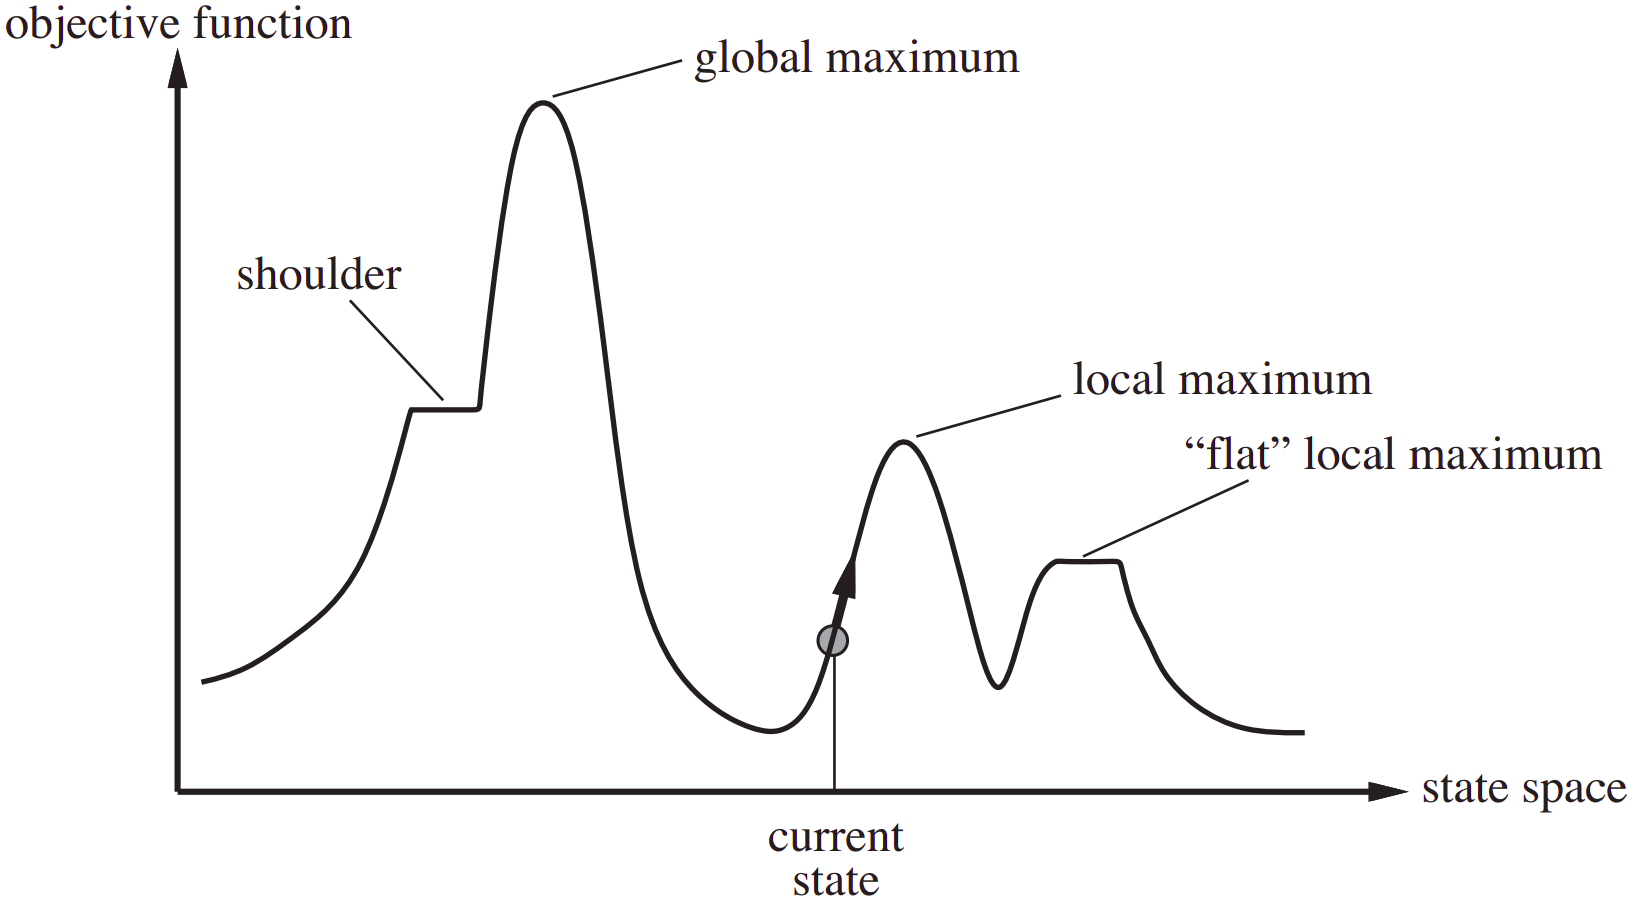
\includegraphics[
        width=\linewidth,
        height=6cm,
        keepaspectratio,
    ]{images/artificial-intelligence/searching/state-space-landscape--objective-function.png}
    \caption*{
        A one-dimensional \textbf{state-space landscape} in which elevation corresponds to the objective function. The aim is to find the global maximum.
        \cite{ai/book/Artificial-Intelligence-A-Modern-Approach/Russell-Norvig}
    }
\end{figure}
\end{minipage}
\hfill
\vrule
\hfill
\begin{minipage}[t]{0.40\linewidth}
\begin{figure}[H]
    \centering
    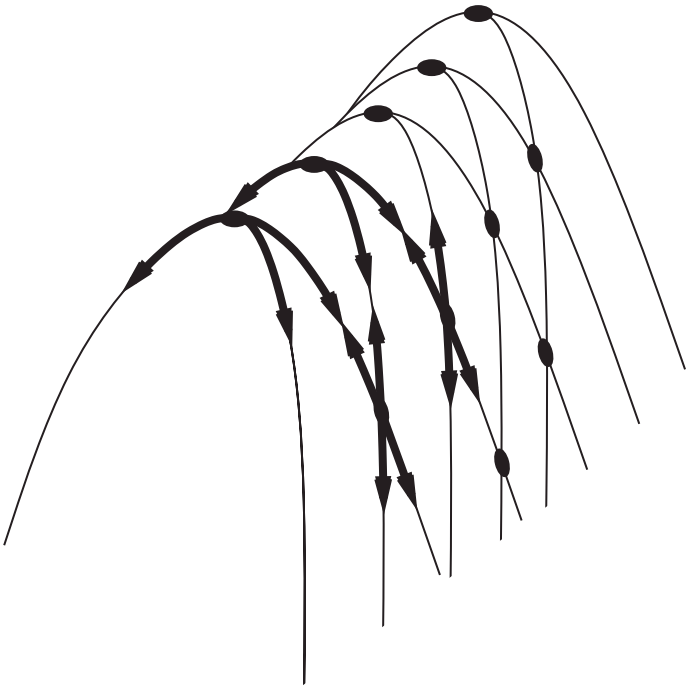
\includegraphics[
        width=\linewidth,
        height=5cm,
        keepaspectratio,
    ]{images/artificial-intelligence/searching/local-search-ridges.png}
    \caption*{
        The grid of states (dark circles) is superimposed on a ridge rising from left to right, creating a sequence of local maxima that are not directly connected to each other. From each local maximum, all the available actions point downhill.
        \cite{ai/book/Artificial-Intelligence-A-Modern-Approach/Russell-Norvig}
    }
\end{figure}
\end{minipage}


\end{table}




\begin{enumerate}
    \item[] {\fontsize{18}{18} \textbf{State-space landscape}}:

    \item A landscape has both “location” (defined by the state) and “elevation” (defined by the value of the heuristic cost function or objective function).
    \hfill \cite{ai/book/Artificial-Intelligence-A-Modern-Approach/Russell-Norvig}

    \item if elevation corresponds to cost, then the aim is to find the lowest valley (\textbf{global minimum})
    \hfill \cite{ai/book/Artificial-Intelligence-A-Modern-Approach/Russell-Norvig}

    \item if elevation corresponds to an objective function, then the aim is to find the highest peak (\textbf{global maximum})
    \hfill \cite{ai/book/Artificial-Intelligence-A-Modern-Approach/Russell-Norvig}

    \item These can convert from one to the other just by inserting a minus sign.
    \hfill \cite{ai/book/Artificial-Intelligence-A-Modern-Approach/Russell-Norvig}


    \item \textbf{Local maxima}: a local maximum is a peak that is higher than each of its neighboring states but lower than the global maximum.
    \hfill \cite{ai/book/Artificial-Intelligence-A-Modern-Approach/Russell-Norvig}

    \item \textbf{Ridges}:  Ridges result in a sequence of local maxima
    \hfill \cite{ai/book/Artificial-Intelligence-A-Modern-Approach/Russell-Norvig}

    \item \textbf{Plateaux}: a plateau is a flat area of the state-space landscape. It can be a \textbf{flat local maximum}, from which no uphill exit exists, or a \textbf{shoulder}, from which progress is possible.
    \hfill \cite{ai/book/Artificial-Intelligence-A-Modern-Approach/Russell-Norvig}







    \vspace{1cm}
    \item[] {\fontsize{18}{18} \textbf{Local Search}}:

    \item evaluates and modifies one or more current states rather than systematically exploring paths from an initial state.
    \hfill \cite{ai/book/Artificial-Intelligence-A-Modern-Approach/Russell-Norvig}

    \item These algorithms are suitable for problems in which all that matters is the solution state, not the path cost to reach it.
    these do not worry about paths at all.
    \hfill \cite{ai/book/Artificial-Intelligence-A-Modern-Approach/Russell-Norvig}

    \item The family of local search algorithms includes methods inspired by statistical physics (simulated annealing) and evolutionary biology (genetic algorithms).
    \hfill \cite{ai/book/Artificial-Intelligence-A-Modern-Approach/Russell-Norvig}

    \item Local search algorithms operate using a \textbf{single current node} (rather than multiple paths) and generally move only to neighbors of that node.
    Typically, the paths followed by the search are \textbf{not retained}.
    \hfill \cite{ai/book/Artificial-Intelligence-A-Modern-Approach/Russell-Norvig}

    \item local search algorithms are useful for solving \textbf{pure optimization problems}, in which the aim is to find the best state according to an \textbf{objective function}.
    \hfill \cite{ai/book/Artificial-Intelligence-A-Modern-Approach/Russell-Norvig}

    \item Many optimization problems do not fit the “standard” search models.
    \textbf{For example}: nature provides an objective function—reproductive fitness—that Darwinian evolution could be seen as attempting to optimize, but there is no “goal test” and no “path cost” for this problem.
    \hfill \cite{ai/book/Artificial-Intelligence-A-Modern-Approach/Russell-Norvig}

    \item  Local search algorithms explore this state-space landscape.
    \hfill \cite{ai/book/Artificial-Intelligence-A-Modern-Approach/Russell-Norvig}

    \item A complete local search algorithm always finds a goal if one exists.
    \hfill \cite{ai/book/Artificial-Intelligence-A-Modern-Approach/Russell-Norvig}

    \item An optimal algorithm always finds a global minimum/ maximum.
    \hfill \cite{ai/book/Artificial-Intelligence-A-Modern-Approach/Russell-Norvig}

    \item Local search algorithms typically use a \textbf{complete-state formulation}.
    \hfill  \cite{ai/book/Artificial-Intelligence-A-Modern-Approach/Russell-Norvig}

    \item \textbf{Advantages}:
    \begin{enumerate}
        \item they use very little memory—usually a constant amount
        \hfill \cite{ai/book/Artificial-Intelligence-A-Modern-Approach/Russell-Norvig}

        \item they can often find reasonable solutions in large or infinite (continuous) state spaces for which systematic algorithms are unsuitable
        \hfill \cite{ai/book/Artificial-Intelligence-A-Modern-Approach/Russell-Norvig}
    \end{enumerate}
\end{enumerate}





\subsection{Online Search}

\begin{enumerate}
    \item agent is faced with a state space that is initially unknown and must be explored.
    \hfill \cite{ai/book/Artificial-Intelligence-A-Modern-Approach/Russell-Norvig}



\end{enumerate}















\chapter{AI: Algorithms}\label{AI: Algorithms}

\begin{customArrayStretch}{1.3}
\begin{table}[H]
\centering
\begin{tabular}{r c p{12cm}}

$V$ & set & set of vertices (nodes) of the graph \\

$E$ & set  & set of edges (links) of the graph \\

$b$ & $\in \mathbb{R}$ & \textbf{branching factor} or maximum number of successors of any node \\

$d$ & $\in \mathbb{R}$ & \textbf{depth} of the \textbf{shallowest goal} node (i.e., the number of steps along the path from the root) \\

$m$ & $\in \mathbb{R}$ & maximum length of any path in the state space \\

$\varepsilon$ & $\in \mathbb{R}$ & minimum step cost (small positive constant) \\

$C$ & $\in \mathbb{R}$ & cost of the solution \\

$C^\ast$ & $\in \mathbb{R}$ & cost of the optimal solution \\

$\ell$ & $\in \mathbb{R}$ & predetermined depth limit \\

$G_n$ & node & goal node closest to $n$ \\

$M$ & $\in \mathbb{R}$ & memory bound \\

$N$ & $\in \mathbb{R}$ & total number of nodes generated \\





\hline





$g(n)$ & $\in \mathbb{R}$ & Path Cost (The \textbf{actual cost} from the \textbfit{start node} to the current node $n$) (Eg: UCS) \\

$h(n)$ & $\in \mathbb{R}$ & Heuristic Estimate (The \textbf{estimated cost} from node $n$ to the \textbfit{goal}) (Eg: GBFS, A*) \\

$f(n)$ & $\in \mathbb{R}$ & Evaluation Function (The \textbf{total estimated cost} of the \textbfit{cheapest solution} through $n$) (Eg: A*) \\

$h^\ast(n)$ & $\in \mathbb{R}$ & actual cost of getting from the root to the goal \\




\hline




$\Delta$ & $\in \mathbb{R}$ & \textbf{absolute error}: $\Delta \equiv h^\ast - h$  \\

$\epsilon$ \textbf{OR} $\Delta_r$ & 
$\in \mathbb{R}$ & 
\textbf{relative error}: $\epsilon \equiv \Delta_r \equiv (h^\ast - h)/h^\ast$ \\


$b^{\Delta_r}$ \textbf{OR} $b^\epsilon$ &
$\in \mathbb{R}$ & 
effective branching factor \\






\end{tabular}
\caption*{Notations}
\end{table}
\end{customArrayStretch}


\begin{enumerate}[itemsep=0.2cm]
    \item \textbf{heuristic function}
    \begin{enumerate}[itemsep=0.2cm]
        \item $h(n)$ = estimated cost of the cheapest path from the state at node $n$ to a goal state
        \hfill \cite{ai/book/Artificial-Intelligence-A-Modern-Approach/Russell-Norvig}

        \item Heuristic functions are the most common form in which additional knowledge of the problem is imparted to the search algorithm. 
        \hfill \cite{ai/book/Artificial-Intelligence-A-Modern-Approach/Russell-Norvig}
        
        \item if $n$ is a goal node, then $h(n)=0$
        \hfill \cite{ai/book/Artificial-Intelligence-A-Modern-Approach/Russell-Norvig}

        \item it depends only on the \textbfit{state} at that node.
        \hfill \cite{ai/book/Artificial-Intelligence-A-Modern-Approach/Russell-Norvig}

        \item the values of heuristic (eg: $h_{SLD}$) \textbf{may not} be computed from the problem description itself. Moreover, it takes a certain amount of experience to know that $h_{SLD}$ is correlated with actual road distances and is, therefore, a useful heuristic.
        \hfill \cite{ai/book/Artificial-Intelligence-A-Modern-Approach/Russell-Norvig}

        \item With a good heuristic function, however, the complexity can be reduced substantially. 
        The amount of the reduction depends on the particular problem and on the quality of the heuristic.
        \hfill \cite{ai/book/Artificial-Intelligence-A-Modern-Approach/Russell-Norvig}

        \item \textbf{admissible heuristic}: An admissible heuristic is one that \textbf{never overestimates} the cost to reach the goal. 
        Admissible heuristics are by nature optimistic because they think the cost of solving the problem is less than it actually is.
        \hfill \cite{ai/book/Artificial-Intelligence-A-Modern-Approach/Russell-Norvig}

        \item \textbf{consistency/ monotonicity}: A heuristic $h(n)$ is consistent if, for every node $n$ and every successor $n^\prime$ of $n$ generated by any action $a$, the estimated cost of reaching the goal from $n$ is no greater than the step cost of getting to $n^\prime$ plus the estimated cost of reaching the goal from $n$:
        \hfill \cite{ai/book/Artificial-Intelligence-A-Modern-Approach/Russell-Norvig}
        \\
        .\hfill $h(n) \leq c(n,\ a,\ n^\prime) + h(n^\prime)$
        \hfill \cite{ai/book/Artificial-Intelligence-A-Modern-Approach/Russell-Norvig}
        \\
        \textbf{every} consistent heuristic is also admissible
        \hfill \cite{ai/book/Artificial-Intelligence-A-Modern-Approach/Russell-Norvig}

        \item Consistency is a stricter requirement than admissibility, but one has to work quite hard to concoct heuristics that are admissible but not consistent.
        \hfill \cite{ai/book/Artificial-Intelligence-A-Modern-Approach/Russell-Norvig}

        \item if $h(n)$ is consistent, then the values of $f(n)$ along any path are non-decreasing
        \hfill \cite{ai/book/Artificial-Intelligence-A-Modern-Approach/Russell-Norvig}

        \item For almost all heuristics in practical use, the absolute error is at least proportional to the path cost $h^\ast$, so $\epsilon$ is constant or growing and the time complexity is exponential in $d$.
        \hfill \cite{ai/book/Artificial-Intelligence-A-Modern-Approach/Russell-Norvig}

        \item When the state space has many goal states - particularly \textbf{near-optimal goal} states - the search process can be led astray from the optimal path and there is an extra cost proportional to the number of goals whose cost is within a factor  of the optimal cost.
        \hfill \cite{ai/book/Artificial-Intelligence-A-Modern-Approach/Russell-Norvig}

        \item experimental measurements of b$^\ast$ on a small set of problems can provide a good guide to the heuristic’s overall usefulness. 
        A well-designed heuristic would have a value of b$^\ast$ close to $1$, allowing fairly large problems to be solved at reasonable computational cost.
        \hfill \cite{ai/book/Artificial-Intelligence-A-Modern-Approach/Russell-Norvig}

        \item \textbf{Dominating heuristic}: if for any node $n$, $h_2(n) \geq h_1(n)$, $h_2$ \textbf{dominates} $h_1$.
        Domination translates directly into efficiency: algorithm using $h_2$ will \textbf{never} expand more nodes than same algorithm using $h_1$ 
        (except possibly for some nodes with $f(n) = C^\ast$).
        \hfill \cite{ai/book/Artificial-Intelligence-A-Modern-Approach/Russell-Norvig}
        \\
        For A$^\ast$ search, every node with $f(n) < C^\ast$ will surely be expanded.
        This is the same as saying that every node with $h(n) < C^\ast - g(n)$ will surely be expanded.
        \hfill \cite{ai/book/Artificial-Intelligence-A-Modern-Approach/Russell-Norvig}
    \end{enumerate}

    \item \textbf{evaluation function}:
    \begin{enumerate}[itemsep=0.2cm]
        \item The evaluation function $f$ is construed/ interpreted as a cost estimate, so the node with the lowest evaluation is expanded first.
        \hfill \cite{ai/book/Artificial-Intelligence-A-Modern-Approach/Russell-Norvig}
        
        \item The choice of $f$ determines the search strategy.
        \hfill \cite{ai/book/Artificial-Intelligence-A-Modern-Approach/Russell-Norvig}

        \item $f(n) = g(n)$ or $h(n)$ or $g(n)+h(n)$ or something else depending on the algorithm

        \item The fact that $f$-costs are \textit{non-decreasing} along any path also means that we can draw \textbf{contours} in the state space, just like the contours in a topographic map. 
        With more accurate heuristics, the bands will stretch toward the goal state and become more narrowly focused around the optimal path.
        \hfill \cite{ai/book/Artificial-Intelligence-A-Modern-Approach/Russell-Norvig}

        \item There can be exponentially many states with $f(n) < C^\ast$ even if the absolute error is bounded by a constant.
        \hfill \cite{ai/book/Artificial-Intelligence-A-Modern-Approach/Russell-Norvig}

        
    \end{enumerate}

    \item memory limitations can make a problem intractable from the point of view of computation time
    \hfill \cite{ai/book/Artificial-Intelligence-A-Modern-Approach/Russell-Norvig}

    \item The effective branching factor can vary across problem instances, but usually it is fairly constant for sufficiently hard problems.
    \hfill \cite{ai/book/Artificial-Intelligence-A-Modern-Approach/Russell-Norvig}
\end{enumerate}





\section{Breadth-first search (BFS) \cite{ai/book/Artificial-Intelligence-A-Modern-Approach/Russell-Norvig}}
\label{AI: Algorithms/Breadth-first search (BFS)}


\begin{figure}[H]
    \centering
    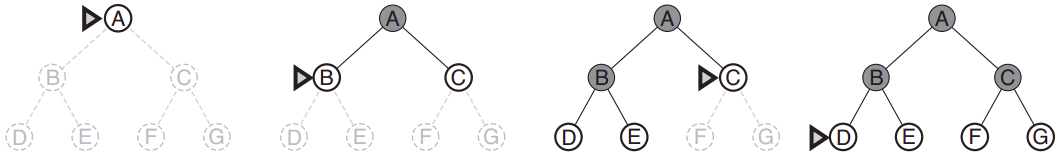
\includegraphics[
        width=\linewidth,
        height=4cm,
        keepaspectratio,
    ]{images/algorithms/Breadth-first-search-BT.png}
    \caption*{
        Breadth-first search on a simple binary tree. At each stage, the node to be expanded next is indicated by a marker.
        \cite{ai/book/Artificial-Intelligence-A-Modern-Approach/Russell-Norvig}
    }
\end{figure}


\begin{enumerate}[itemsep=0.2cm]
    \item Breadth-first search is a simple strategy in which the root node is expanded first, then all the successors of the root node are expanded next, then their successors, and so on. 
    \hfill \cite{ai/book/Artificial-Intelligence-A-Modern-Approach/Russell-Norvig}

    \item In general, all the nodes are expanded at a given depth in the search tree before any nodes at the next level are expanded.
    \hfill \cite{ai/book/Artificial-Intelligence-A-Modern-Approach/Russell-Norvig}

    \item Breadth-first search is an instance of the general graph-search algorithm in which the \textit{shallowest unexpanded node} is chosen for expansion.
    \hfill \cite{ai/book/Artificial-Intelligence-A-Modern-Approach/Russell-Norvig}

    \item new nodes (which are always deeper than their parents) go to the back of the queue, and old nodes, which are shallower than the new nodes, get expanded first. 
    \hfill \cite{ai/book/Artificial-Intelligence-A-Modern-Approach/Russell-Norvig}

    \item There is one slight tweak on the general graph-search algorithm, which is that the goal test is applied to each node when it is generated rather than when it is selected for expansion.
    \hfill \cite{ai/book/Artificial-Intelligence-A-Modern-Approach/Russell-Norvig}
    \\
    If the algorithm were to apply the goal test to nodes when selected for expansion, rather than when generated, the whole layer of nodes at depth d would be expanded before the goal was detected and the time complexity would be $\mathcal{O}(b\ ^{d+1})$.
    \hfill \cite{ai/book/Artificial-Intelligence-A-Modern-Approach/Russell-Norvig}

    \item the algorithm, following the general template for graph search, discards any new path to a state already in the frontier or explored set; it is easy to see that any such path must be at least as deep as the one already found. 
    \hfill \cite{ai/book/Artificial-Intelligence-A-Modern-Approach/Russell-Norvig}

    \item breadth-first search \textbf{always} has the \textit{shallowest path} to every node on the frontier. 
    As soon as a goal node is generated, we know it is the shallowest goal node because all shallower nodes must have been generated already and failed the goal test. 
    \hfill \cite{ai/book/Artificial-Intelligence-A-Modern-Approach/Russell-Norvig}

    \item \textbf{performance}:
    \begin{enumerate}[itemsep=0.2cm]
        \item \textbf{complete}: if the shallowest goal node is at some finite depth $d$, breadth-first search will eventually find it after generating all shallower nodes (provided the branching factor $b$ is finite). 
        \hfill \cite{ai/book/Artificial-Intelligence-A-Modern-Approach/Russell-Norvig}

        \item  the shallowest goal node is \textbf{not necessarily} the \textit{optimal} one. 
        breadth-first search is optimal if the path cost is a non-decreasing function of the depth of the node.
        The most common such scenario is that all actions have the same cost.
        the algorithm is optimal if step costs are all identical.
        \hfill \cite{ai/book/Artificial-Intelligence-A-Modern-Approach/Russell-Norvig}

        \item \textbf{Space Complexity}:
        \begin{enumerate}[itemsep=0.1cm]
            \item explored set: $\mathcal{O}(b\ ^{d-1})$
            \hfill \cite{ai/book/Artificial-Intelligence-A-Modern-Approach/Russell-Norvig}

            \item frontier: $\mathcal{O}(b\ ^{d})$
            \hfill \cite{ai/book/Artificial-Intelligence-A-Modern-Approach/Russell-Norvig}

            \item overall: $\mathcal{O}(b\ ^{d})$
            \hfill \cite{ai/book/Artificial-Intelligence-A-Modern-Approach/Russell-Norvig}
        \end{enumerate}

        \item \textbf{Time Complexity}: 
        $\mathcal{O}(b\ ^{d})$
        \hfill \cite{ai/book/Artificial-Intelligence-A-Modern-Approach/Russell-Norvig}

    \end{enumerate}

    \item \textbf{Disadvantages}:
    \begin{enumerate}[itemsep=0.1cm]
        \item the memory requirements are a bigger problem for breadth-first search than is the execution time.
        \hfill \cite{ai/book/Artificial-Intelligence-A-Modern-Approach/Russell-Norvig}

        
    \end{enumerate}

\end{enumerate}


\subsection*{Implementation}

\begin{enumerate}
    \item \textbf{frontier}: FIFO queue
\end{enumerate}


\vspace{0.5cm}


\begin{algorithm}[H]
    \caption{Breadth-first search on a graph. \cite{ai/book/Artificial-Intelligence-A-Modern-Approach/Russell-Norvig}}

    \SetKwFunction{FUNCTION}{\textsc{Breadth-First-Search}}
    \SetKwProg{Fn}{function}{ returns \normalfont{a solution, or failure}}{end}
    \Fn{\FUNCTION{problem}}{
        $node \ \gets$ a node with \textsc{State} = $problem$.\textsc{Initial-State}, \textsc{Path-Cost} = $0$ \\
        \ \\
        \If{$problem$.\textsc{Goal-Test}($node$.\textsc{State})}{
            \Return \textsc{Solution}($node$)
        }
        \ \\
        $frontier \ \gets$ a FIFO queue with node as the only element \\
        $explored \ \gets$ an empty set \\
        \ \\
        \While{}{
            \If{\textsc{Empty?}($frontier$)}{
                \Return failure
            }
            \ \\
            \Comment{chooses the shallowest node in $frontier$}
            $node \ \gets$ \textsc{Pop}($frontier$) \\ 
            add $node$.\textsc{State} to $explored$ \\
            \ \\
            \ForEach{$action$ \textbf{in} $problem$.\textsc{Actions}($node$.\textsc{State})}{
                $child \gets$ \textsc{Child-Node}($problem,\ node,\ action$) \\
                \If{$child$.\textsc{State} is \textbf{not in} $explored$ or $frontier$}{
                    \If{$problem$.\textsc{Goal-Test}($child$.\textsc{State})}{
                        \Return \textsc{Solution}($child$)
                    }
                    $frontier \gets$ \textsc{Insert}($child,\ frontier$)
                }
            }
        }
    }
\end{algorithm}


\begin{lstlisting}[
    language=Python,
    caption=Problem Solving Agent - Breadth-first search on a graph
]
from queue import Queue

def breadth_first_search(problem: Problem):
    node = Node(problem.initial_state, None, None, 0)

    if problem.goal_test(node.state):
        return solution(node)
    
    frontier = Queue()
    explored = set()

    frontier.put(node)

    while True:
        if frontier.empty():
            return None
        
        node = frontier.get()
        explored.add(node)

        for action in problem.actions(node.state):
            child = child_node(problem, node, action)
            
            if (not any([n.state == child.state for n in frontier.queue]) and 
                not any([n.state == child.state for n in explored])):
                if problem.goal_test(child.state):            
                    return solution(child)

                frontier.put(child)
\end{lstlisting}












\section{Uniform-cost search (UCS) \cite{ai/book/Artificial-Intelligence-A-Modern-Approach/Russell-Norvig}}
\label{AI: Algorithms/Uniform-cost search (UCS)}


\begin{enumerate}[itemsep=0.2cm]
    \item Instead of expanding the shallowest node (as in BFS), uniform-cost search expands the node $n$ with the \textbfit{lowest path cost} $g(n)$.
    \hfill \cite{ai/book/Artificial-Intelligence-A-Modern-Approach/Russell-Norvig}

    \item \textbf{Performance}:
    \begin{enumerate}[itemsep=0.2cm]
        \item uniform-cost search is \textbf{optimal} in general. 
        uniform-cost search expands nodes in order of their optimal path cost.
        \hfill \cite{ai/book/Artificial-Intelligence-A-Modern-Approach/Russell-Norvig}

        \item \textbf{Completeness is guaranteed} provided the cost of every step exceeds some small positive constant $\varepsilon$ and $b$ is finite
        \hfill \cite{ai/book/Artificial-Intelligence-A-Modern-Approach/Russell-Norvig}

        \item \textbf{Space Complexity}:
        \begin{enumerate}[itemsep=0.2cm]
            \item worst: $\mathcal{O}(b^{1 + \dfloor{C^\ast / \varepsilon}})$
            \hfill (can be much greater than $b^d$)
            \hfill \cite{ai/book/Artificial-Intelligence-A-Modern-Approach/Russell-Norvig}

            \item When all step costs are equal: $\mathcal{O}(b^{\ d+1})$
            \hfill \cite{ai/book/Artificial-Intelligence-A-Modern-Approach/Russell-Norvig}
        \end{enumerate}

        \item \textbf{Time Complexity}:
        \begin{enumerate}[itemsep=0.2cm]
            \item worst: $\mathcal{O}(b^{1 + \dfloor{C^\ast / \varepsilon}})$
            \hfill (can be much greater than $b^d$)
            \hfill \cite{ai/book/Artificial-Intelligence-A-Modern-Approach/Russell-Norvig}

            \item When all step costs are equal: $\mathcal{O}(b^{\ d+1})$
            \hfill \cite{ai/book/Artificial-Intelligence-A-Modern-Approach/Russell-Norvig}
        \end{enumerate}
    \end{enumerate}

    \item \textbf{Disadvantages}:
    \begin{enumerate}[itemsep=0.2cm]
        \item it will get stuck in an \textbf{infinite loop} if there is a path with an infinite sequence of \textit{zero-cost actions} - for example, a sequence of $NoOp$ actions.
        \hfill \cite{ai/book/Artificial-Intelligence-A-Modern-Approach/Russell-Norvig}

        \item  it suffers from the same difficulties with realvalued costs
        \hfill \cite{ai/book/Artificial-Intelligence-A-Modern-Approach/Russell-Norvig}
    \end{enumerate}

    \item When all step costs are the same, uniform-cost search is similar to breadth-first search, except that the latter stops as soon as it generates a goal, whereas uniform-cost search examines all the nodes at the goal’s depth to see if one has a lower cost; thus uniform-cost search does strictly more work by expanding nodes at depth $d$ unnecessarily.
    \hfill \cite{ai/book/Artificial-Intelligence-A-Modern-Approach/Russell-Norvig}
\end{enumerate}




\subsection*{Implementation}

\begin{enumerate}
    \item  This is done by storing the frontier as a \textbf{priority queue} ordered by $g(n)$. 
    \hfill \cite{ai/book/Artificial-Intelligence-A-Modern-Approach/Russell-Norvig}

    \item In addition to the ordering of the queue by path cost, there are two other significant differences from breadth-first search.
    \hfill \cite{ai/book/Artificial-Intelligence-A-Modern-Approach/Russell-Norvig}
    \begin{enumerate}
        \item  goal test is applied to a node when it is \textit{selected for expansion} rather than when it is first generated.
        The reason is that the first goal node that is \textit{generated} may be on a suboptimal path.
        \hfill \cite{ai/book/Artificial-Intelligence-A-Modern-Approach/Russell-Norvig}

        \item a test is added in case a better path is found to a node currently on the frontier.
        \hfill \cite{ai/book/Artificial-Intelligence-A-Modern-Approach/Russell-Norvig}
    \end{enumerate}

\end{enumerate}

\vspace{0.5cm}


\begin{algorithm}[H]
    \caption{\textsc{Uniform-Cost} search on a graph. \cite{ai/book/Artificial-Intelligence-A-Modern-Approach/Russell-Norvig}}

    \SetKwFunction{FUNCTION}{\textsc{Uniform-Cost-Search}}
    \SetKwProg{Fn}{function}{ returns \normalfont{a solution, or failure}}{end}
    \Fn{\FUNCTION{problem}}{
        $node \ \gets$ a node with \textsc{State} = $problem$.\textsc{Initial-State}, \textsc{Path-Cost} = $0$ \\
        $frontier \ \gets$ a \textbfit{priority queue} ordered by \textsc{Path-Cost}, with $node$ as the only element \\
        $explored \ \gets$ an empty set \\
        \ \\
        \While{}{
            \lIf{\textsc{Empty?}($frontier$)}{
                \Return failure
            }
            \Comment{chooses the lowest-cost node in $frontier$}
            $node \ \gets$ \textsc{Pop}($frontier$) \\ 
            \lIf{$problem$.\textsc{Goal-Test}($node$.\textsc{State})}{
                \Return \textsc{Solution}($node$)
            }
            add $node$.\textsc{State} to $explored$ \\
            \ \\
            \ForEach{$action$ \textbf{in} $problem$.\textsc{Actions}($node$.\textsc{State})}{
                $child \gets$ \textsc{Child-Node}($problem,\ node,\ action$) \\
                \If{\normalfont $child$.\textsc{State} is not in $explored$ or $frontier$}{
                    $frontier \gets$ \textsc{Insert}($child,\ frontier$)
                }
                \ElseIf{\normalfont $child$.\textsc{State} is in $frontier$ with higher \textsc{Path-Cost}}{
                    replace that $frontier$ node with $child$
                }
            }
        }
    }
\end{algorithm}


\begin{lstlisting}[
    language=Python,
    caption=Problem Solving Agent - Uniform cost search on a graph
]
import heapq

def uniform_cost_search(problem: Problem):
    node = Node(problem.initial_state, None, None, 0)

    if problem.goal_test(node.state):
        return solution(node)
    
    frontier = [(node.path_cost, node)]
    explored = set()

    heapq.heapify(frontier)

    while True:
        if len(frontier) == 0:
            return None
        
        path_cost, node = frontier.pop(0)

        if problem.goal_test(node.state):
            return solution(node)

        explored.add(node)
        for action in problem.actions(node.state):
            child = child_node(problem, node, action)

            if (not any([n.state == child.state for (path_cost, n) in frontier])
                and not any([n.state == child.state for n in explored])):
                frontier.append((child.path_cost, child))
                heapq.heapify(frontier)
            else:
                for idx, (path_cost, n) in enumerate(frontier):
                    if n.state == child.state and path_cost > child.path_cost:
                        frontier[idx] = (child.path_cost, child)
                        heapq.heapify(frontier)
\end{lstlisting}






\section{Depth-first search (DFS) \cite{ai/book/Artificial-Intelligence-A-Modern-Approach/Russell-Norvig}}


\begin{figure}[H]
\centering
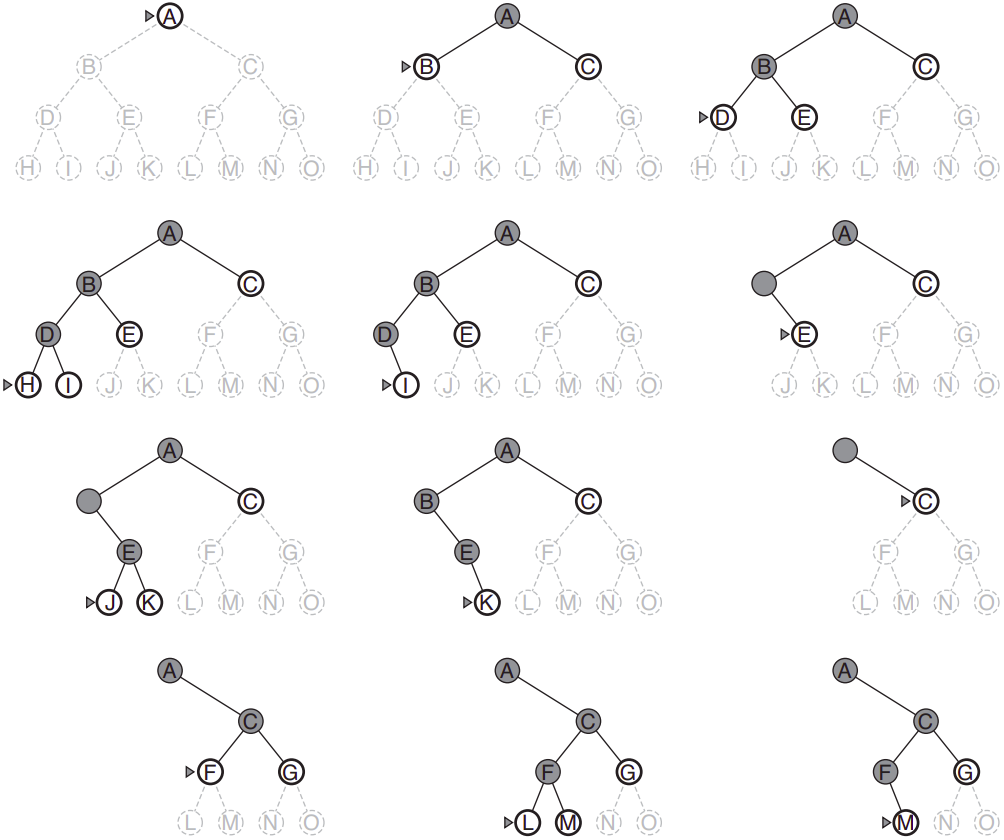
\includegraphics[
    width=\linewidth,
    height=7cm,
    keepaspectratio,
]{images/algorithms/Depth-first-search-illustration.png}
\caption*{
    Depth-first search on a binary tree. The unexplored region is shown in light gray. Explored nodes with no descendants in the frontier are removed from memory. Nodes at depth $3$ have no successors and $M$ is the only goal node. 
    \cite{ai/book/Artificial-Intelligence-A-Modern-Approach/Russell-Norvig}
}
\end{figure}


\begin{enumerate}[itemsep=0.2cm]
    \item Depth-first search always expands the \textbf{deepest node} in the current frontier of the search tree.
    \hfill \cite{ai/book/Artificial-Intelligence-A-Modern-Approach/Russell-Norvig}

    \item The search proceeds immediately to the deepest level of the search tree, where the nodes have no successors. As those nodes are expanded, they are dropped from the frontier, so then the search “backs up” to the next deepest node that still has unexplored successors.
    \hfill \cite{ai/book/Artificial-Intelligence-A-Modern-Approach/Russell-Norvig}

    \item \textbf{Performance}:
    \begin{enumerate}[itemsep=0.2cm]
        \item \textbf{graph-search version}:
        \begin{enumerate}[itemsep=0.2cm]
            \item \textbf{complete} in finite state spaces because it will eventually expand every node
            \hfill \cite{ai/book/Artificial-Intelligence-A-Modern-Approach/Russell-Norvig}

            \item \textbf{not optimal}
            \hfill \cite{ai/book/Artificial-Intelligence-A-Modern-Approach/Russell-Norvig}

            \item \textbf{time complexity}: $\mathcal{O}(b^d)$
            \hfill \cite{ai/book/Artificial-Intelligence-A-Modern-Approach/Russell-Norvig}

            \item \textbf{space complexity}: $\mathcal{O}(b^d)$
            \hfill \cite{ai/book/Artificial-Intelligence-A-Modern-Approach/Russell-Norvig}
        \end{enumerate}

        \item \textbf{tree-search version}:
        \begin{enumerate}[itemsep=0.2cm]
            \item \textbf{not complete}, as it can fall in \textit{infinite loop}
            \hfill \cite{ai/book/Artificial-Intelligence-A-Modern-Approach/Russell-Norvig}

            \item \textbf{not optimal}
            \hfill \cite{ai/book/Artificial-Intelligence-A-Modern-Approach/Russell-Norvig}

            \item \textbf{time complexity}: $\mathcal{O}(b^m)$
            \hfill \cite{ai/book/Artificial-Intelligence-A-Modern-Approach/Russell-Norvig}

            \item \textbf{space complexity}: $\mathcal{O}(b\ m)$
            \hfill \cite{ai/book/Artificial-Intelligence-A-Modern-Approach/Russell-Norvig}
        \end{enumerate}
    \end{enumerate}
\end{enumerate}


\subsection{Implementation}

\begin{enumerate}[itemsep=0.2cm]
    \item The depth-first search algorithm is an instance of the graph-search algorithm that uses a LIFO queue.
    \hfill \cite{ai/book/Artificial-Intelligence-A-Modern-Approach/Russell-Norvig}

    \item  it is common to implement depth-first search with a recursive function that calls itself  on each of its children in turn. 
    \hfill \cite{ai/book/Artificial-Intelligence-A-Modern-Approach/Russell-Norvig}
\end{enumerate}

\begin{lstlisting}[
    language=Python,
    caption=Problem Solving Agent - Depth first search on a graph
]
from queue import LifoQueue

def depth_first_search(problem: Problem):
    node = Node(problem.initial_state, None, None, 0)

    if problem.goal_test(node.state):
        return solution(node)
    
    frontier = LifoQueue()
    explored = set()

    frontier.put(node)

    while True:
        if frontier.empty():
            return None
        
        node = frontier.get()
        explored.add(node)

        for action in problem.actions(node.state):
            child = child_node(problem, node, action)

            if (not any([n.state == child.state for n in frontier.queue]) and 
                not any([n.state == child.state for n in explored])):
                if problem.goal_test(child.state):
                    return solution(child)

                frontier.put(child)
\end{lstlisting}















\section{Backtracking Search \cite{ai/book/Artificial-Intelligence-A-Modern-Approach/Russell-Norvig}}
\label{AI: Algorithms/Backtracking Search}


\begin{enumerate}
    \item A variant of depth-first search that uses still less memory.
    \hfill \cite{ai/book/Artificial-Intelligence-A-Modern-Approach/Russell-Norvig}

    \item \textbf{only one successor} is generated at a time rather than all successors; each partially expanded node remembers which successor to generate next.
    \hfill \cite{ai/book/Artificial-Intelligence-A-Modern-Approach/Russell-Norvig}

    \item \textbf{Performance}:
    \begin{enumerate}
        \item \textbf{Space Complexity}: $\mathcal{O}(m)$
        \hfill \cite{ai/book/Artificial-Intelligence-A-Modern-Approach/Russell-Norvig}
    \end{enumerate}

    \item \textbf{Advantages}:
    \begin{enumerate}
        \item  Backtracking search facilitates memory-saving (and time-saving) trick: the idea of generating a successor by \textbf{modifying} the current state description directly rather than copying it first.
        For this to work, we must be able to \textbf{undo} each modification when we go back to generate the next successor.
        \hfill \cite{ai/book/Artificial-Intelligence-A-Modern-Approach/Russell-Norvig}

        \item For problems with large state descriptions, such as robotic assembly, these techniques are critical to success.
        \hfill \cite{ai/book/Artificial-Intelligence-A-Modern-Approach/Russell-Norvig}
    \end{enumerate}
\end{enumerate}



\begin{lstlisting}[
    language=Python,
    caption=Problem Solving Agent - Backtracking using recursion \cite{common/online/chatgpt}
]
def backtrack(node: Node, explored: set):
    if problem.goal_test(node.state):
        return solution(node)

    explored.add(node)

    for action in problem.actions(node.state):
        child = child_node(problem, node, action)
        if not any([child.state == n.state for n in explored]):
            result = backtrack(child, explored)
            if result is not None:
                return result

    # Optional: allow revisiting for other paths (depends on problem)
    explored.remove(node)
    return None

def backtracking_search(problem: Problem):
    root = Node(problem.initial_state, None, None, 0)
    return backtrack(root, set())
\end{lstlisting}















\section{Depth-limited search \cite{ai/book/Artificial-Intelligence-A-Modern-Approach/Russell-Norvig}}

\begin{enumerate}[itemsep=0.2cm]
    \item The embarrassing failure of depth-first search in infinite state spaces can be alleviated by supplying depth-first search with a predetermined depth limit $\ell$. That is, nodes at depth  $\ell$ are treated as if they have no successors. 
    \hfill \cite{ai/book/Artificial-Intelligence-A-Modern-Approach/Russell-Norvig}

    \item \textbf{Performance}:
    \begin{enumerate}
        \item \textbf{Completeness}: NO \textbf{if} $\ell < d$ \textbf{else} YES
        \hfill \cite{ai/book/Artificial-Intelligence-A-Modern-Approach/Russell-Norvig}

        \item \textbf{Optimal}: NO \textbf{if} $\ell > d$ \textbf{else} YES
        \hfill \cite{ai/book/Artificial-Intelligence-A-Modern-Approach/Russell-Norvig}

        \item \textbf{time complexity}: $\mathcal{O}(b^\ell)$
        \hfill \cite{ai/book/Artificial-Intelligence-A-Modern-Approach/Russell-Norvig}

        \item \textbf{space complexity}: $\mathcal{O}(b\ell)$
        \hfill \cite{ai/book/Artificial-Intelligence-A-Modern-Approach/Russell-Norvig}
    \end{enumerate}

    \item Depth-first search can be viewed as a special case of depth-limited search with $\ell = \infty$.
    \hfill \cite{ai/book/Artificial-Intelligence-A-Modern-Approach/Russell-Norvig}

    \item diameter of the state space can be a better limit for efficiency
    \hfill \cite{ai/book/Artificial-Intelligence-A-Modern-Approach/Russell-Norvig}

    
\end{enumerate}


\vspace{0.5cm}

\begin{algorithm}[H]
    \caption{A recursive implementation of depth-limited tree search. \cite{ai/book/Artificial-Intelligence-A-Modern-Approach/Russell-Norvig}}


    \SetKwFunction{FUNCTION}{\textsc{Depth-Limited-Search}}
    \SetKwProg{Fn}{function}{ returns \normalfont{a solution, or failure/cutoff}}{end}
    \Fn{\FUNCTION{problem, limit}}{
        \Return \textsc{Recursive-DLS}( \\
            \hspace{0.5cm}  \textsc{Make-Node}($problem$.\textsc{Initial-State}), \\
            \hspace{0.5cm}  $problem$, \\
            \hspace{0.5cm}  $limit$, \\
        )
    }
    
    \ \\
    
    \SetKwFunction{FUNCTION}{\textsc{Recursive-DLS}}
    \SetKwProg{Fn}{function}{ returns \normalfont{a solution, or failure/cutoff}}{end}
    \Fn{\FUNCTION{node, problem, limit}}{
        \If{\normalfont $problem$.\textsc{Goal-Test}($node$.\textsc{State})}{
            \Return \textsc{Solution}($node$) 
        }
        \ElseIf{limit = 0}{
            \Return $cutoff$
        }
        \Else{
            $cutoff\_occurred? \ \gets$ false\\
            \ \\
            \ForEach{\normalfont $action$ \textbf{in} $problem$.\textsc{Actions}($node$.\textsc{State})}{
                $child \gets$ \textsc{Child-Node}($problem,\ node,\ action$)\\
                $result \gets$ \textsc{Recursive-DLS}($child,\ problem,\ limit-1$)\\
                \If{result = cutoff}{
                    $cutoff\_occurred? \ \gets$ true
                }
                \ElseIf{result $\neq$ failure}{
                    \Return $result$
                }
            }
            \ \\
            \If{$cutoff\_occurred?$}{
                \Return $cutoff$
            }
            \Else{
                \Return $failure$
            }
        }
    }
\end{algorithm}


\begin{lstlisting}[
    language=Python,
    caption=Problem Solving Agent - Depth limited search (recursive)
]
CUTOFF = "CUT-OFF"

def depth_limited_search(problem: Problem, limit: int):
    return recursive_dls(
        Node(problem.initial_state, None, None, 0),
        problem,
        limit,
    )

def recursive_dls(node: Node, problem: Problem, limit: int):
    if problem.goal_test(node.state):
        return solution(node)
    
    elif limit == 0:
        return CUTOFF
    
    else:
        cutoff_occurred = False
        for action in problem.actions(node.state):
            child = child_node(problem, node, action)
            result = recursive_dls(child, problem, limit-1)
            if result == CUTOFF:
                cutoff_occurred = True
            elif result is not None:
                return result
        if cutoff_occurred:
            return CUTOFF
        else:
            return
\end{lstlisting}


\vspace{0.5cm}

\begin{enumerate}[itemsep=0.2cm]
    \item $failure$ value indicates no solution
    \hfill \cite{ai/book/Artificial-Intelligence-A-Modern-Approach/Russell-Norvig}

    \item $cutoff$ value indicates no solution within the depth limit
    \hfill \cite{ai/book/Artificial-Intelligence-A-Modern-Approach/Russell-Norvig}
\end{enumerate}








\section{Iterative Deepening Search (IDS) \cite{ai/book/Artificial-Intelligence-A-Modern-Approach/Russell-Norvig}}
\label{AI: Algorithms/Iterative Deepening Search (IDS)}


\begin{figure}[h!]
    \centering
    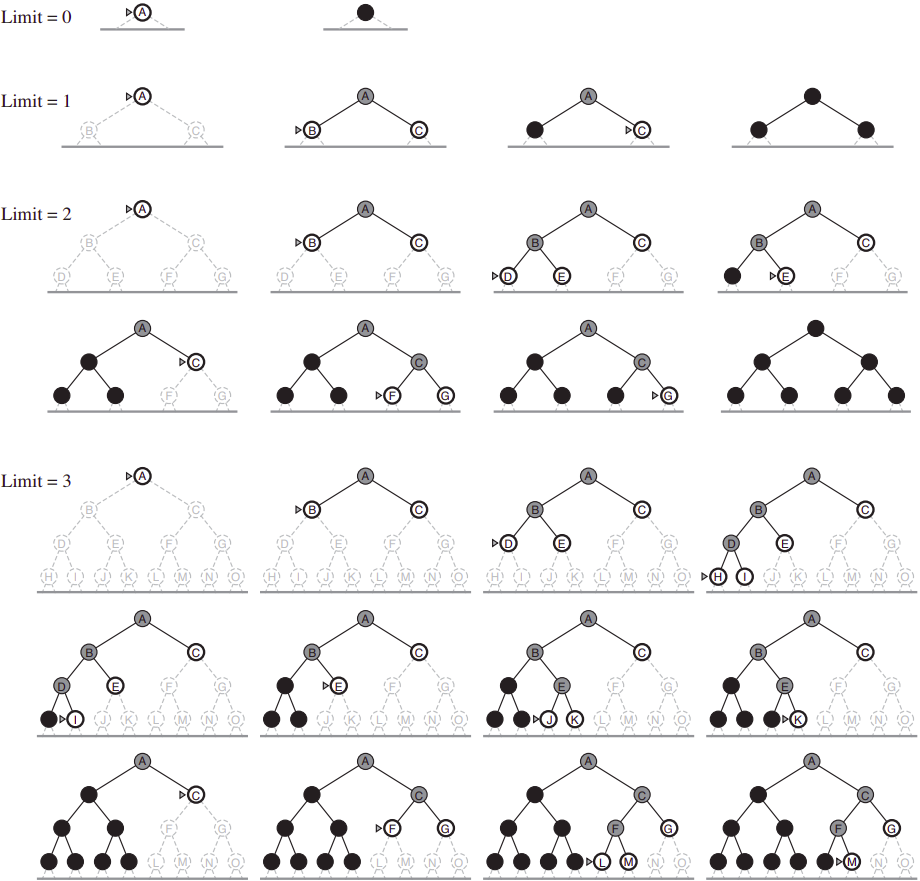
\includegraphics[
        width=\linewidth,
        height=14cm,
        keepaspectratio,
    ]{images/algorithms/iterative-deepening-search-BT.png}
    \caption*{Four iterations of iterative deepening search on a binary tree \cite{ai/book/Artificial-Intelligence-A-Modern-Approach/Russell-Norvig}}
\end{figure}


\begin{enumerate}
    \item \textbf{Iterative deepening search} (or \textbf{iterative deepening depth-first search}) is a general strategy, often used in combination with depth-first tree search, that finds the best depth limit.
    \hfill \cite{ai/book/Artificial-Intelligence-A-Modern-Approach/Russell-Norvig}

    \item It gradually increases the depth limit $\ell \in \dCurlyBrac{0,1,2,\cdots,\infty}$ till a goal is found, which occurs when $\ell = d$ ($d$ is unknown in reality)
    \hfill \cite{ai/book/Artificial-Intelligence-A-Modern-Approach/Russell-Norvig}

    \item Iterative deepening combines the benefits of depth-first and breadth-first search.
    \hfill \cite{ai/book/Artificial-Intelligence-A-Modern-Approach/Russell-Norvig}
    \begin{enumerate}
        \item Like depth-first search, its memory requirements are modest: $\mathcal{O}(b d)$ to be precise. 
        \hfill \cite{ai/book/Artificial-Intelligence-A-Modern-Approach/Russell-Norvig}

        \item Like breadth-first search, it is complete when the branching factor is finite and optimal when the path cost is a non-decreasing function of the depth of the node.
        \hfill \cite{ai/book/Artificial-Intelligence-A-Modern-Approach/Russell-Norvig}
    \end{enumerate}

    \item total number of nodes generated in the worst case is
    \\
    $N(\text{IDS})=(d)b + (d - 1)b^2 + \cdots + (1)b^d$
    \hfill \cite{ai/book/Artificial-Intelligence-A-Modern-Approach/Russell-Norvig}

    \item you can use a hybrid approach that runs breadth-first search until almost all the available memory is consumed, and then runs iterative deepening from all the nodes in the frontier.
    \hfill \cite{ai/book/Artificial-Intelligence-A-Modern-Approach/Russell-Norvig}

    \item iterative deepening is the \textit{preferred uninformed search} method when the search space is large and the depth of the solution is not known.
    \hfill \cite{ai/book/Artificial-Intelligence-A-Modern-Approach/Russell-Norvig}

    \item \textbf{Performance}:
    \begin{enumerate}
        \item \textbf{completeness}: YES \textbf{if} $b$ is finite \textbf{else} NO
        \hfill \cite{ai/book/Artificial-Intelligence-A-Modern-Approach/Russell-Norvig}

        \item \textbf{optimal}: YES \textbf{if} path cost is a non-deceasing function of depth of the node \textbf{else} NO
        \hfill \cite{ai/book/Artificial-Intelligence-A-Modern-Approach/Russell-Norvig}
        
        \item \textbf{space complexity}: $\mathcal{O}(b d)$
        \hfill \cite{ai/book/Artificial-Intelligence-A-Modern-Approach/Russell-Norvig}

        \item \textbf{time complexity}: $\mathcal{O}(b^d)$
        \hfill \cite{ai/book/Artificial-Intelligence-A-Modern-Approach/Russell-Norvig}
    \end{enumerate}
\end{enumerate}

\vspace{0.5cm}

\begin{algorithm}[H]
    \caption{The iterative deepening search algorithm, which repeatedly applies depth-limited search with increasing limits. It terminates when a solution is found or if the depth-limited search returns failure, meaning that no solution exists. \cite{ai/book/Artificial-Intelligence-A-Modern-Approach/Russell-Norvig}}

    \SetKwFunction{FUNCTION}{\textsc{Iterative-Deepening-Search}}
    \SetKwProg{Fn}{function}{ returns \normalfont{a solution, or failure}}{end}
    \Fn{\FUNCTION{problem}}{
        \For{\normalfont $depth = 0$ \textbf{to} $\infty$}{
            $result \gets$ \textsc{Depth-Limited-Search}($problem,\ depth$)\\
            \lIf{$result \neq cutoff$}{
                \Return $result$
            }
        }
    }
\end{algorithm}


\begin{lstlisting}[
    language=Python,
    caption=Problem Solving Agent - Iterative Deepening Search 
]
def iterative_deepening_search(problem: Problem, limit=1000000):
    for i in range(limit):
        result = depth_limited_search(problem, i)
        if result != CUTOFF:
            return result
\end{lstlisting}







\section{Iterative Lengthening Search (ILS) \cite{ai/book/Artificial-Intelligence-A-Modern-Approach/Russell-Norvig}}
\label{AI: Algorithms/Iterative Lengthening Search (ILS)}


\begin{enumerate}
    \item an iterative analog to uniform-cost search, inheriting the Iterative deepening search algorithm’s optimality guarantees while avoiding its memory requirements. The idea is to use increasing path-cost limits instead of increasing depth limits.
    \hfill \cite{ai/book/Artificial-Intelligence-A-Modern-Approach/Russell-Norvig}

    \item \textbf{Disadvantage}: It turns out that iterative lengthening incurs substantial overhead compared to uniform-cost search.
    \hfill \cite{ai/book/Artificial-Intelligence-A-Modern-Approach/Russell-Norvig}
\end{enumerate}


\vspace{0.5cm}


\begin{lstlisting}[
    language=Python,
    caption=Problem Solving Agent - Iterative Lengthening Search \cite{common/online/chatgpt}
]
def iterative_lengthening_search(problem: Problem):
    cost_limit = 0

    while True:
        result, new_cost_limit = uniform_cost_search_with_cost_limit(
            problem,
            cost_limit,
        )

        if result is not None:
            return result

        if new_cost_limit == float('inf'):
            return None

        cost_limit = new_cost_limit


def uniform_cost_search_with_cost_limit(problem: Problem, cost_limit: int):
    node = Node(problem.initial_state, None, None, 0)

    if problem.goal_test(node.state):
        return solution(node), cost_limit

    frontier = [(node.path_cost, node)]
    explored = set()
    heapq.heapify(frontier)
    next_cost_limit = float('inf')

    while frontier:
        path_cost, node = heapq.heappop(frontier)

        if path_cost > cost_limit:
            next_cost_limit = min(next_cost_limit, path_cost)
            continue

        if problem.goal_test(node.state):
            return solution(node), cost_limit

        explored.add(node)

        for action in problem.actions(node.state):
            child = child_node(problem, node, action)

            if (not any(child.state == n.state for n in explored) and
                not any(n.state == child.state for _, n in frontier)):
                heapq.heappush(frontier, (child.path_cost, child))

    return None, next_cost_limit
\end{lstlisting}







\section{Bidirectional search \cite{ai/book/Artificial-Intelligence-A-Modern-Approach/Russell-Norvig}}
\label{AI: Algorithms/Bidirectional search}

\begin{figure}[h!]
    \centering
    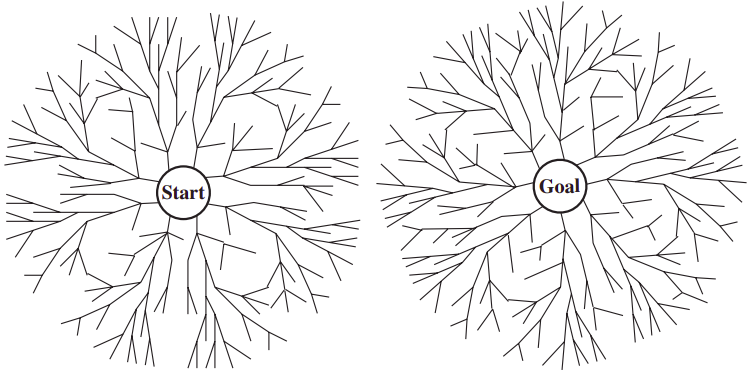
\includegraphics[
        width=\linewidth,
        height=4cm,
        keepaspectratio,
    ]{images/algorithms/bidirectional-search-illustration.png}
    \caption*{A schematic view of a bidirectional search that is about to succeed when a branch from the start node meets a branch from the goal node. \cite{ai/book/Artificial-Intelligence-A-Modern-Approach/Russell-Norvig}}
\end{figure}


\begin{enumerate}[itemsep=0.2cm]
    \item The idea behind bidirectional search is to run two simultaneous searches - one forward from the initial state and the other backward from the goal - hoping that the two searches meet in the middle
    \hfill \cite{ai/book/Artificial-Intelligence-A-Modern-Approach/Russell-Norvig}

    \item The motivation is that $b^{d/2} + b^{d/2}$ is much less than $b^d$
    \hfill \cite{ai/book/Artificial-Intelligence-A-Modern-Approach/Russell-Norvig}

    \item Bidirectional search is implemented by replacing the goal test with a check to see whether the frontiers of the two searches intersect; if they do, a solution has been found.
    \hfill \cite{ai/book/Artificial-Intelligence-A-Modern-Approach/Russell-Norvig}

    \item The check can be done when each node is generated or selected for expansion and, with a hash table, will take constant time.
    \hfill \cite{ai/book/Artificial-Intelligence-A-Modern-Approach/Russell-Norvig}

    \item \textbf{predecessors} of a state $x$ be all those states that have $x$ as a successor. Bidirectional search requires a method for computing predecessors. When all the actions in the state space are reversible, the predecessors of $x$ are just its successors. 
    \hfill \cite{ai/book/Artificial-Intelligence-A-Modern-Approach/Russell-Norvig}

    \item \textbf{Performance}:
    \begin{enumerate}
        \item \textbf{optimality}: 
        \begin{enumerate}
            \item YES \textbf{if} additional search is used to make sure the path isn’t another short-cut across the gap \textbf{else} NO
            \hfill \cite{ai/book/Artificial-Intelligence-A-Modern-Approach/Russell-Norvig}

            \item YES \textbf{if}  step costs are all identical \textbfit{and} both directions use breadth-first search \textbf{else} NO
            \hfill \cite{ai/book/Artificial-Intelligence-A-Modern-Approach/Russell-Norvig}
        \end{enumerate}

        \item \textbf{completeness}: YES \textbf{if} $b$ is finite \textbfit{and} both directions use breadth-first search \textbf{else} NO
        \hfill \cite{ai/book/Artificial-Intelligence-A-Modern-Approach/Russell-Norvig}

        \item \textbf{space complexity}:
        \begin{enumerate}
            \item using breadth-first searches in both directions: $\mathcal{O}(b^{d/2})$
            \hfill \cite{ai/book/Artificial-Intelligence-A-Modern-Approach/Russell-Norvig}
        \end{enumerate}

        \item \textbf{time complexity}:
        \begin{enumerate}
            \item using breadth-first searches in both directions: $\mathcal{O}(b^{d/2})$
            \hfill \cite{ai/book/Artificial-Intelligence-A-Modern-Approach/Russell-Norvig}
        \end{enumerate}
    \end{enumerate}
\end{enumerate}

























\section{Best-first search (BestFS) \cite{ai/book/Artificial-Intelligence-A-Modern-Approach/Russell-Norvig}}
\label{AI: Algorithms/Best-first search (BestFS)}


\begin{enumerate}
    \item Best-first search is an instance of the general \textsc{Tree-Search} or \textsc{Graph-Search} algorithm in which a node is selected for expansion based on an \textbf{evaluation function}, $f(n)$. $f(n)$ can be any function that returns a value for a given node.
    \hfill \cite{ai/book/Artificial-Intelligence-A-Modern-Approach/Russell-Norvig}

    \item The implementation of best-first graph search is identical to that for uniform-cost search, except for the use of $f$ instead of $g$ to order the priority queue.
    \hfill \cite{ai/book/Artificial-Intelligence-A-Modern-Approach/Russell-Norvig}

    \item Most best-first algorithms include $h$ as a component of $f$
    \hfill \cite{ai/book/Artificial-Intelligence-A-Modern-Approach/Russell-Norvig}
\end{enumerate}


\begin{lstlisting}[
    language=Python,
    caption=Problem Solving Agent - (General) Best-first search (BestFS) on a graph
]
def best_first_search(problem: Problem, f):
    node = Node(problem.initial_state, None, None, 0)

    if problem.goal_test(node.state):
        return solution(node)

    frontier = [(f(node), node)]
    heapq.heapify(frontier)
    explored = set()

    while frontier:
        _, node = heapq.heappop(frontier)

        if problem.goal_test(node.state):
            return solution(node)

        explored.add(node)

        for action in problem.actions(node.state):
            child = child_node(problem, node, action)
            if (all(n.state != child.state for n in explored) 
                and all(n.state != child.state for _, n in frontier)):
                heapq.heappush(frontier, (f(child), child))
            else:
                # Optional: Replace in frontier if better
                for i, (old_f, old_node) in enumerate(frontier):
                    if old_node.state == child.state and f(child) < old_f:
                        frontier[i] = (f(child), child)
                        heapq.heapify(frontier)
                        break

    return None
\end{lstlisting}





\section{Greedy best-first search (GBFS) \cite{ai/book/Artificial-Intelligence-A-Modern-Approach/Russell-Norvig}}
\label{AI: Algorithms/Greedy best-first search (GBFS)}

.\hfill
$f(n) = h(n)$
\hfill \cite{ai/book/Artificial-Intelligence-A-Modern-Approach/Russell-Norvig}

\ \\

\begin{enumerate}
    \item Greedy best-first search tries to expand the node that is \textbf{closest} to the goal, on the grounds that this is likely to lead to a solution quickly.
    \hfill \cite{ai/book/Artificial-Intelligence-A-Modern-Approach/Russell-Norvig}

    \item at each step it tries to get as close to the goal as it can
    \hfill \cite{ai/book/Artificial-Intelligence-A-Modern-Approach/Russell-Norvig}

    \item \textbf{Performance}:
    \begin{enumerate}
        \item \textbf{Completeness}: YES \textbf{if} graph version is used \textbf{and} states are finite \textbf{else} NO
        \hfill \cite{ai/book/Artificial-Intelligence-A-Modern-Approach/Russell-Norvig}

        \item \textbf{time complexity}
        \begin{enumerate}
            \item worst case: $\mathcal{O}(b^m)$
            \hfill \cite{ai/book/Artificial-Intelligence-A-Modern-Approach/Russell-Norvig}
        \end{enumerate}

        \item \textbf{space complexity}
        \begin{enumerate}
            \item worst case: $\mathcal{O}(b^m)$
            \hfill \cite{ai/book/Artificial-Intelligence-A-Modern-Approach/Russell-Norvig}
        \end{enumerate}
    \end{enumerate}
\end{enumerate}




\begin{lstlisting}[
    language=Python,
    caption=Problem Solving Agent - Greedy Best-first search (GBFS) on a graph
]
import heapq

def greedy_best_first_search(problem: Problem):
    node = Node(problem.initial_state, None, None, 0)

    if problem.goal_test(node.state):
        return solution(node)

    # Priority queue ordered by heuristic cost
    frontier = [(problem.heuristic(node.state), node)]
    heapq.heapify(frontier)

    explored = set()

    while len(frontier) > 0:
        _, node = heapq.heappop(frontier)

        if problem.goal_test(node.state):
            return solution(node)

        explored.add(node)

        for action in problem.actions(node.state):
            child = child_node(problem, node, action)
            h_cost = problem.heuristic(child.state)

            # Add child only if it's not in frontier or explored
            in_frontier = any(n.state == child.state for _, n in frontier)
            in_explored = any(n.state == child.state for n in explored)

            if not in_frontier and not in_explored:
                heapq.heappush(frontier, (h_cost, child))
            else:
                # Optional: If it's in the frontier but has a
                # better heuristic, replace it
                for idx, (old_cost, old_node) in enumerate(frontier):
                    if old_node.state == child.state and h_cost < old_cost:
                        frontier[idx] = (h_cost, child)
                        heapq.heapify(frontier)
                        break

    return None  # No solution found

# Greedy Best-First Search using general best first search
greedy_best_first_search_alt = lambda problem: best_first_search(
    problem,
    f=lambda n: problem.heuristic(n.state)
)
\end{lstlisting}











\section{A$^\ast$ Search \cite{ai/book/Artificial-Intelligence-A-Modern-Approach/Russell-Norvig}}
\label{AI: Algorithms/A* Search}

.\hfill
$f(n) = g(n) + h(n)$
\hfill \cite{ai/book/Artificial-Intelligence-A-Modern-Approach/Russell-Norvig}

\ \\

\begin{enumerate}[itemsep=0.2cm]
    \item It evaluates nodes by combining $g(n)$, the cost to reach the node, and $h(n)$, the cost to get from the node to the goal ($f(n)$ = estimated cost of the cheapest solution through $n$)
    \hfill \cite{ai/book/Artificial-Intelligence-A-Modern-Approach/Russell-Norvig}

    \item A$^\ast$ selects a node $n$ for expansion, the optimal path to that node has been found
    \hfill \cite{ai/book/Artificial-Intelligence-A-Modern-Approach/Russell-Norvig}

    \item Because A$^\ast$ expands the frontier node of lowest $f$-cost, we can see that an A$^\ast$ search fans out from the start node, adding nodes in \textbf{concentric bands} of increasing $f$-cost.
    \hfill \cite{ai/book/Artificial-Intelligence-A-Modern-Approach/Russell-Norvig}

    \item If $C^\ast$ is the cost of the optimal solution path, then we can say the following:
    \begin{enumerate}[itemsep=0.2cm]
        \item A$^\ast$ expands all nodes with $f(n) < C^\ast$
        \hfill \cite{ai/book/Artificial-Intelligence-A-Modern-Approach/Russell-Norvig}

        \item A$^\ast$ might then expand some of the nodes right on the “goal contour” (where $f(n) = C^\ast$) before selecting a goal node.
        \hfill \cite{ai/book/Artificial-Intelligence-A-Modern-Approach/Russell-Norvig}
    \end{enumerate}

    \item if $h(n)$ is admissible, the algorithm can safely \textbf{ignore/ prune} this sub-tree while still guaranteeing optimality
    \hfill \cite{ai/book/Artificial-Intelligence-A-Modern-Approach/Russell-Norvig}

    \item  among optimal algorithms of this type - algorithms that extend search paths from the root and use the same heuristic information - A$^\ast$ is \textbf{optimally efficient} for any given consistent heuristic.
    \hfill \cite{ai/book/Artificial-Intelligence-A-Modern-Approach/Russell-Norvig}

    \item best results follow the 3 assumptions:
    \begin{enumerate}
        \item Single goal state
        \hfill \cite{ai/book/Artificial-Intelligence-A-Modern-Approach/Russell-Norvig}
        
        \item Tree structure
        \hfill \cite{ai/book/Artificial-Intelligence-A-Modern-Approach/Russell-Norvig}
        
        \item Reversible actions
        \hfill \cite{ai/book/Artificial-Intelligence-A-Modern-Approach/Russell-Norvig}
    \end{enumerate}

    \item \textbf{Performance}:
    \begin{enumerate}[itemsep=0.2cm]
        \item the \textit{tree-search} version of A$^\ast$ is \textbf{optimal} if $h(n)$ is admissible, 
        while the \textit{graph-search} version is \textbf{optimal} if $h(n)$ is consistent
        \hfill \cite{ai/book/Artificial-Intelligence-A-Modern-Approach/Russell-Norvig}

        \item \textbf{Completeness} requires that there be only finitely many nodes with cost less than or equal to $C^\ast$, a condition that is true if all step costs exceed some finite  and if $b$ is finite.
        \hfill \cite{ai/book/Artificial-Intelligence-A-Modern-Approach/Russell-Norvig}

        \item \textbf{time complexity}:
        \begin{enumerate}
            \item in maximum absolute error: $\mathcal{O}(b^\Delta)$
            \hfill \cite{ai/book/Artificial-Intelligence-A-Modern-Approach/Russell-Norvig}
            
            \item constant step costs: $\mathcal{O}(b^{\Delta_rd})$ or $\mathcal{O}(b^{\epsilon d})$
            \hfill \cite{ai/book/Artificial-Intelligence-A-Modern-Approach/Russell-Norvig}
        \end{enumerate}
    \end{enumerate}

    \item \textbf{Disadvantages}
    \begin{enumerate}
        \item for most problems, the number of states within the goal contour search space is still \textbf{exponential} in the length of the solution
        \hfill \cite{ai/book/Artificial-Intelligence-A-Modern-Approach/Russell-Norvig}

        \item Because it keeps all generated nodes in memory (as do all \textsc{Graph-Search} algorithms), A$^\ast$ usually runs out of space long before it runs out of time.
        \hfill \cite{ai/book/Artificial-Intelligence-A-Modern-Approach/Russell-Norvig}

        \item A$^\ast$ is not practical for many large-scale problems. 
        \hfill \cite{ai/book/Artificial-Intelligence-A-Modern-Approach/Russell-Norvig}

        \item The existence of an effective branching factor follows from the result that the number of nodes expanded by A$^\ast$ grows exponentially with solution depth.
        \hfill \cite{ai/book/Artificial-Intelligence-A-Modern-Approach/Russell-Norvig}
    \end{enumerate}
\end{enumerate}


\vspace{0.5cm}

\begin{lstlisting}[
    language=Python,
    caption=Problem Solving Agent - A* search \cite{common/online/chatgpt}
]
def a_star_search(problem: Problem):
    start_node = Node(problem.initial_state, None, None, 0)

    if problem.goal_test(start_node.state):
        return solution(start_node)

    # Priority queue ordered by f(n) = g(n) + h(n)
    frontier = [(problem.heuristic(start_node.state), start_node)]
    heapq.heapify(frontier)

    explored = dict()  # {state: path_cost}

    while len(frontier)> 0:
        f, current = heapq.heappop(frontier)

        if problem.goal_test(current.state):
            return solution(current)

        # If this state has already been explored with a lower cost, skip
        if any(n.state == current.state for n in explored) and explored[current] <= current.path_cost:
            continue

        explored[current] = current.path_cost

        for action in problem.actions(current.state):
            child = child_node(problem, current, action)
            f_child = child.path_cost + problem.heuristic(child.state)

            # Check if child.state was already explored with a lower path_cost
            if (any(n.state == child.state for n in explored) or 
                explored[child] > child.path_cost):
                heapq.heappush(frontier, (f_child, child))

    return None  # No solution found

# A* Search using general best first search
a_star_search_alt = lambda problem: best_first_search(
    problem, 
    f=lambda n: n.path_cost + problem.heuristic(n.state)
)
\end{lstlisting}












\section{Iterative-Deepening A$^\ast$ (IDA$^\ast$) search \cite{ai/book/Artificial-Intelligence-A-Modern-Approach/Russell-Norvig}}
\label{AI: Algorithms/Iterative-Deepening A* search}


\begin{enumerate}

\item adapt the idea of iterative deepening to the heuristic search context
\hfill \cite{ai/book/Artificial-Intelligence-A-Modern-Approach/Russell-Norvig}

\item The main difference between IDA$^\ast$ and standard iterative deepening is that the cutoff used is the $f$-cost ($g + h$) rather than the depth
\hfill \cite{ai/book/Artificial-Intelligence-A-Modern-Approach/Russell-Norvig}

\item at each iteration, the cutoff value is the smallest $f$-cost of any node that exceeded the cutoff on the previous iteration
\hfill \cite{ai/book/Artificial-Intelligence-A-Modern-Approach/Russell-Norvig}

\item IDA$^\ast$ is practical for many problems with unit step costs and avoids the substantial overhead associated with keeping a sorted queue of nodes. 
\hfill \cite{ai/book/Artificial-Intelligence-A-Modern-Approach/Russell-Norvig}

\item \textbf{Disadvantages}:
\begin{enumerate}
    \item  it suffers from the same difficulties with real-valued costs
    \hfill \cite{ai/book/Artificial-Intelligence-A-Modern-Approach/Russell-Norvig}

    \item suffer from using too little memory.
    \hfill \cite{ai/book/Artificial-Intelligence-A-Modern-Approach/Russell-Norvig}

    \item may end up re-expanding the same states many times over
    \hfill \cite{ai/book/Artificial-Intelligence-A-Modern-Approach/Russell-Norvig}

    \item suffer the potentially exponential increase in complexity associated with redundant paths in graphs
    \hfill \cite{ai/book/Artificial-Intelligence-A-Modern-Approach/Russell-Norvig}
\end{enumerate}

\end{enumerate}




\begin{lstlisting}[
    language=Python,
    caption=Problem Solving Agent - Iterative-Deepening A$^\ast$ (IDA$^\ast$)
]
def ida_star_search(problem: Problem):
    """
    Performs Iterative Deepening A* Search.
    Returns the solution as a list of actions, or None if no solution is found.
    """

    start_node = Node(problem.initial_state, None, None, 0)
    bound = problem.heuristic(start_node.state)

    while True:
        result = _ida_search(start_node, problem, bound)

        if isinstance(result, list):  # Found a solution
            return result

        if result == float('inf'):
            return None  # No solution

        bound = result  # Increase bound and try again


def _ida_search(node: Node, problem: Problem, bound: float):
    """
    Helper function for IDA* search.
    Returns either:
    - A solution path (list of actions), or
    - The next bound (float) to use in the next iteration
    """
    f = node.path_cost + problem.heuristic(node.state)

    if f > bound:
        return f

    if problem.goal_test(node.state):
        return solution(node)

    min_threshold = float('inf')
    for action in problem.actions(node.state):
        child = child_node(problem, node, action)
        result = _ida_search(child, problem, bound)

        if isinstance(result, list):
            return result  # Solution found

        if result < min_threshold:
            min_threshold = result

    return min_threshold
\end{lstlisting}












\section{Recursive best-first search (RBFS) \cite{ai/book/Artificial-Intelligence-A-Modern-Approach/Russell-Norvig}}
\label{AI: Algorithms/Recursive best-first search (RBFS)}


\begin{enumerate}[itemsep=0.2cm]
    \item simple recursive algorithm that attempts to mimic the operation of standard best-first search, but using only \textbf{linear space}
    \hfill \cite{ai/book/Artificial-Intelligence-A-Modern-Approach/Russell-Norvig}

    \item Its structure is similar to that of a recursive depth-first search, but rather than continuing indefinitely down the current path, it uses the $f\_limit$ variable to keep track of the $f$-value of the best \textbf{alternative} path available from any ancestor of the current node. 
    If the current node exceeds this limit, the recursion unwinds back to the alternative path.
    \hfill \cite{ai/book/Artificial-Intelligence-A-Modern-Approach/Russell-Norvig}

    \item As the recursion unwinds, RBFS replaces the f-value of each node along the path with a \textbf{backed-up value} - the best f-value of its children. 
    In this way, RBFS remembers the $f$-value of the best leaf in the forgotten sub-tree and can therefore decide whether it’s worth re-expanding the sub-tree at some later time.
    \hfill \cite{ai/book/Artificial-Intelligence-A-Modern-Approach/Russell-Norvig}

    \item RBFS is somewhat more \textbf{efficient} than IDA$^\ast$
    \hfill \cite{ai/book/Artificial-Intelligence-A-Modern-Approach/Russell-Norvig}

    \item \textbf{Disadvantages}:
    \begin{enumerate}
        \item suffers from excessive node regeneration
        \hfill \cite{ai/book/Artificial-Intelligence-A-Modern-Approach/Russell-Norvig}
    \end{enumerate}
\end{enumerate}


\vspace{0.5cm}

\begin{algorithm}[H]
    \caption{The algorithm for recursive best-first search. \cite{ai/book/Artificial-Intelligence-A-Modern-Approach/Russell-Norvig}}


    \SetKwFunction{FUNCTION}{\textsc{Recursive-Best-First-Search}}
    \SetKwProg{Fn}{function}{ returns \normalfont{a solution, or failure}}{end}
    \Fn{\FUNCTION{problem}}{
        \Return \textsc{RBFS}(\\
            \hspace{0.5cm} $problem$, \\
            \hspace{0.5cm} \textsc{Make-Node}($problem$.\textsc{Initial-State}), \\
            \hspace{0.5cm} $\infty$, \\
        )
    }
    
    \ \\
    
    \SetKwFunction{FUNCTION}{\textsc{RBFS}}
    \SetKwProg{Fn}{function}{ returns \normalfont{a solution, or failure and a new f-cost limit}}{end}
    \Fn{\FUNCTION{problem}}{
        \lIf{$problem$.\textsc{Goal-Test}($node$.\textsc{State})}{
            \Return \textsc{Solution}($node$)
        }
        $successors$ $\gets$ [] \\
        \ForEach{\normalfont $action$ \textbf{in} $problem$.\textsc{Actions}($node$.\textsc{State})}{
            add \textsc{Child-Node}($problem,\ node,\ action$) \textbf{into} $successors$
        }
        \lIf{\normalfont $successors$ is empty}{
            \Return $failure,\ \infty$
        }
        \Comment{update $f$ with value from previous search, if any}
        \lForEach{\normalfont $s$ \textbf{in} $successors$}{
            $s.f$ $\gets$ max($s.g + s.h$, $node.f$)
        }
        \ \\
        \While{}{
            $best$ $\gets$ the lowest $f$-value node in $successors$ \\
            \lIf{$best.f > f\_limit$}{
                \Return $failure$, $best.f$
            }
            $alternative$ $\gets$ the second-lowest $f$-value among \textbf{successors} \\
            $result,\ best.f$ $\gets$ \textsc{RBFS}($problem$, $best$, min($f\_limit,\ alternative$)) \\
            \lIf{result $\neq$ failure}{
                \Return $result$
            }
        }
    }
\end{algorithm}










\section{Memory-Bounded A$^\ast$ (MA$^\ast$) Search \cite{ai/book/Artificial-Intelligence-A-Modern-Approach/Russell-Norvig}}
\label{AI: Algorithms/Memory-Bounded A* (MA*) Search}


\begin{enumerate}
    \item 
    \hfill \cite{ai/book/Artificial-Intelligence-A-Modern-Approach/Russell-Norvig}
\end{enumerate}








\section{Simplified Memory-Bounded A$^\ast$ (SMA$^\ast$) Search \cite{ai/book/Artificial-Intelligence-A-Modern-Approach/Russell-Norvig}}
\label{AI: Algorithms/Simplified Memory-Bounded A* (SMA*) Search}


\begin{enumerate}
    \item SMA$^\ast$ proceeds just like A$^\ast$, expanding the best leaf until memory is full.
    At this point, it cannot add a new node to the search tree without dropping an old one.
    SMA$^\ast$ always drops the \textbf{worst leaf node}—the one with the highest $f$-value.
    \hfill \cite{ai/book/Artificial-Intelligence-A-Modern-Approach/Russell-Norvig}

    \item  Like RBFS, SMA$^\ast$ then backs up the value of the forgotten node to its parent.
    In this way, the ancestor of a forgotten sub-tree knows the quality of the best path in that sub-tree.
    SMA$^\ast$ regenerates the sub-tree only when all other paths have been shown to look worse than the path it has forgotten.
    \hfill \cite{ai/book/Artificial-Intelligence-A-Modern-Approach/Russell-Norvig}

    \item  if all the descendants of a node $n$ are forgotten, then we will not know which way to go from $n$, but we will still have an idea of how worthwhile it is to go anywhere from $n$.
    \hfill \cite{ai/book/Artificial-Intelligence-A-Modern-Approach/Russell-Norvig}

    \item if all the leaf nodes have the same f-value, SMA$^\ast$ expands the \textbf{newest best} leaf and deletes the \textbf{oldest worst} leaf to avoid selecting the same node for deletion and expansion
    \hfill \cite{ai/book/Artificial-Intelligence-A-Modern-Approach/Russell-Norvig}

    \item If the leaf is not a goal node, then even if it is on an optimal solution path, that solution is not reachable with the available memory.
    Therefore, the node can be discarded exactly as if it had no successors.
    \hfill \cite{ai/book/Artificial-Intelligence-A-Modern-Approach/Russell-Norvig}

    \item In practical terms, SMA$^\ast$ is a fairly robust choice for finding optimal solutions, particularly when the state space is a graph, step costs are not uniform, and node generation is expensive compared to the overhead of maintaining the frontier and the explored set.
    \hfill \cite{ai/book/Artificial-Intelligence-A-Modern-Approach/Russell-Norvig}

    \item \textbf{Disadvantages}:
    \begin{enumerate}
        \item On very hard problems, it will often be the case that SMA$^\ast$ is forced to switch back and forth continually among many candidate solution paths, only a small subset of which can fit in memory.
        \hfill \cite{ai/book/Artificial-Intelligence-A-Modern-Approach/Russell-Norvig}

        \item the extra time required for repeated regeneration of the same nodes means that problems that would be practically solvable by A$^\ast$, given unlimited memory, become intractable for SMA$^\ast$.
        \hfill \cite{ai/book/Artificial-Intelligence-A-Modern-Approach/Russell-Norvig}
    \end{enumerate}
\end{enumerate}











\clearpage
\section{Summary}


\begin{customArrayStretch}{1.7}
\begin{longtable}{| 
>{\RaggedRight\arraybackslash}p{5cm} | 
>{\RaggedRight\arraybackslash}p{1.5cm} | 
>{\RaggedRight\arraybackslash}p{3cm} | 
>{\centering\arraybackslash}p{1cm} | 
>{\centering\arraybackslash}p{1cm} | 
>{\centering\arraybackslash}p{1cm} | 
>{\centering\arraybackslash}p{0.7cm} |}

\hline
\multirow{2}{*}{\textbf{Algorithm}} & 
\multirow{2}{*}{\textbf{Complete?}} &
\multirow{2}{*}{\textbf{Optimal?}} & 
\multicolumn{2}{c|}{\textbf{Time Complexity}} &
\multicolumn{2}{c|}{\textbf{Space Complexity}}
\\ \cline{4-7}
&&& 
\textbf{Graph} & \textbf{Tree} & 
\textbf{Graph} & \textbf{Tree}
\\ \hline
\endfirsthead

\hline
\multirow{2}{*}{\textbf{Algorithm}} & 
\multirow{2}{*}{\textbf{Complete?}} &
\multirow{2}{*}{\textbf{Optimal?}} & 
\multicolumn{2}{c|}{\textbf{Time Complexity}} &
\multicolumn{2}{c|}{\textbf{Space Complexity}}
\\ \cline{4-7}
&&& 
\textbf{Graph} & \textbf{Tree} & 
\textbf{Graph} & \textbf{Tree}
\\ \hline
\endhead

\hline\endfoot
\hline\endlastfoot


%%%%%%%%%%%%%%%%%%%%%%%%%%%%%%%%%%%%%%%%%%%%%%%%

\multicolumn{7}{|c|}{\fontsize{17}{17}\selectfont \textsc{Uninformed Search/ Blind Search}} \\ \hline

%%%%%%%%%%%%%%%%%%%%%%%%%%%%%%%%%%%%%%%%%%%%%%%%

\hyperref[AI: Algorithms/Breadth-first search (BFS)]{\textbf{Breadth-first search (BFS)}} &
YES$^3$ &
YES$^{1|2}$ &
\multicolumn{2}{c|}{$\mathcal{O}(b^d)$} &
\multicolumn{2}{c|}{$\mathcal{O}(b^d)$}
\\ \hline


\hyperref[AI: Algorithms/Uniform-cost search (UCS)]{\textbf{Uniform-cost search (UCS)}} &
YES$^4$ &
YES &
\multicolumn{2}{c|}{$\mathcal{O}(b^{1+\dfloor{C^\ast/\varepsilon}})$} &
\multicolumn{2}{c|}{$\mathcal{O}(b^{1+\dfloor{C^\ast/\varepsilon}})$}
\\ \hline


\hyperref[AI: Algorithms/Depth-first search (DFS)]{\textbf{Depth-first search (DFS)}} &
YES$^{3\&5}$ &
NO &
$\mathcal{O}(b^d)$ & $\mathcal{O}(b^m)$ &
$\mathcal{O}(bd)$ & $\mathcal{O}(bm)$
\\ \hline


\hyperref[AI: Algorithms/Backtracking Search]{\textbf{Backtracking Search}} &
YES$^{3\&5}$ &
NO &
$\mathcal{O}(b^d)$ & $\mathcal{O}(b^m)$ &
$\mathcal{O}(d)$ & $\mathcal{O}(m)$
\\ \hline


\hyperref[AI: Algorithms/Depth-limited search (DLS)]{\textbf{Depth-limited search (DLS)}} &
NO$^{6}$ &
YES$^{6}$ &
\multicolumn{2}{c|}{$\mathcal{O}(b^\ell)$} &
\multicolumn{2}{c|}{$\mathcal{O}(b\ell)$}
\\ \hline


\hyperref[AI: Algorithms/Iterative Deepening Search (IDS)]{\textbf{Iterative Deepening Search (IDS)}} &
YES$^{3}$ &
YES$^{1|2}$ &
\multicolumn{2}{c|}{$\mathcal{O}(b^d)$} &
\multicolumn{2}{c|}{$\mathcal{O}(bd)$}
\\ \hline


\hyperref[AI: Algorithms/Iterative Lengthening Search (ILS)]{\textbf{Iterative Lengthening Search (ILS)}} &
YES$^{4}$ &
YES &
\multicolumn{2}{c|}{$\mathcal{O}(b^{1+\dfloor{C^\ast/\varepsilon}})$} &
\multicolumn{2}{c|}{$\mathcal{O}(bC^\ast/\varepsilon)$}
\\ \hline


\hyperref[AI: Algorithms/Bidirectional search]{\textbf{Bidirectional search}} &
YES$^{7}$ &
YES$^{2\&8}$ &
\multicolumn{2}{c|}{$\mathcal{O}(b^{d/2})$} &
\multicolumn{2}{c|}{$\mathcal{O}(b^{d/2})$}
\\ \hline


%%%%%%%%%%%%%%%%%%%%%%%%%%%%%%%%%%%%%%%%%%%%%%%%

\multicolumn{7}{|c|}{\fontsize{17}{17}\selectfont \textsc{Informed Search/ Heuristic Search}} 
\\ \hline

%%%%%%%%%%%%%%%%%%%%%%%%%%%%%%%%%%%%%%%%%%%%%%%%


\hyperref[AI: Algorithms/Greedy best-first search (GBFS)]{\textbf{Greedy best-first search (GBFS)}} &
YES$^{3\&5}$ &
NO &
\multicolumn{2}{c|}{$\mathcal{O}(b^m)$} &
\multicolumn{2}{c|}{$\mathcal{O}(b^m)$}
\\ \hline


\hyperref[AI: Algorithms/A* Search]{\textbf{A* Search}} &
YES$^{3\&4}$ &
YES$^{(9\&10)|(5\&11)}$ &
\multicolumn{2}{c|}{$\mathcal{O}(
    b^\Delta)^{12}$ or 
    $\mathcal{O}(b^{\Delta_rd})^{2}$
} &
\multicolumn{2}{c|}{$\mathcal{O}()$}
\\ \hline













\end{longtable}
\end{customArrayStretch}

\vspace{0.5cm}
\textbf{Conditions}:
\vspace{0.2cm}
\begin{enumerate}[itemsep=0.1cm]
% 1
\item path cost is a non-decreasing function of the depth of the node
% 2
\item step costs are all identical
% 3
\item branching factor $b$ is finite (number of states are finite)
% 4
\item every step exceeds some small positive constant $\varepsilon > 0$
% 5
\item graph version is used
% 6
\item $\ell < d$
% 7
\item additional search is used to make sure the path isn’t another short-cut across the gap
% 8
\item both directions use breadth-first search
% 9
\item tree version is used
% 10
\item $h(n)$ is admissible
% 11
\item $h(n)$ is consistent
% 12
\item in the maximum absolute error
\end{enumerate}


\vspace{0.5cm}
\textbf{Notation Interpretation}:
\vspace{0.2cm}
\begin{enumerate}[itemsep=0.2cm]

\item YES$^{a|b}$ = YES \textbf{if} either $a$ \textbf{or} $b$ must satisfy \textbf{else} NO

\item YES$^{a\&b}$ = YES \textbf{if} either $a$ \textbf{and} $b$ must satisfy \textbf{else} NO

\end{enumerate}

















\chapter{AI: Examples}
\section{Vacuum Cleaner (Toy problem) \cite{ai/book/Artificial-Intelligence-A-Modern-Approach/Russell-Norvig}}


\begin{figure}[H]
    \centering
    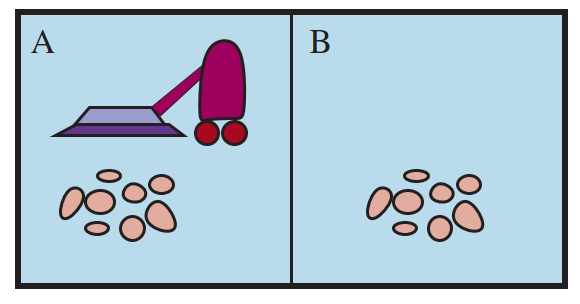
\includegraphics[
        width=0.5\linewidth,
        height=3cm,
        keepaspectratio
    ]{images/artificial-intelligence/examples/vacuum-cleaner-world.png}
    \caption{A vacuum-cleaner world with just two locations}
\end{figure}

\begin{figure}[H]
    \centering
    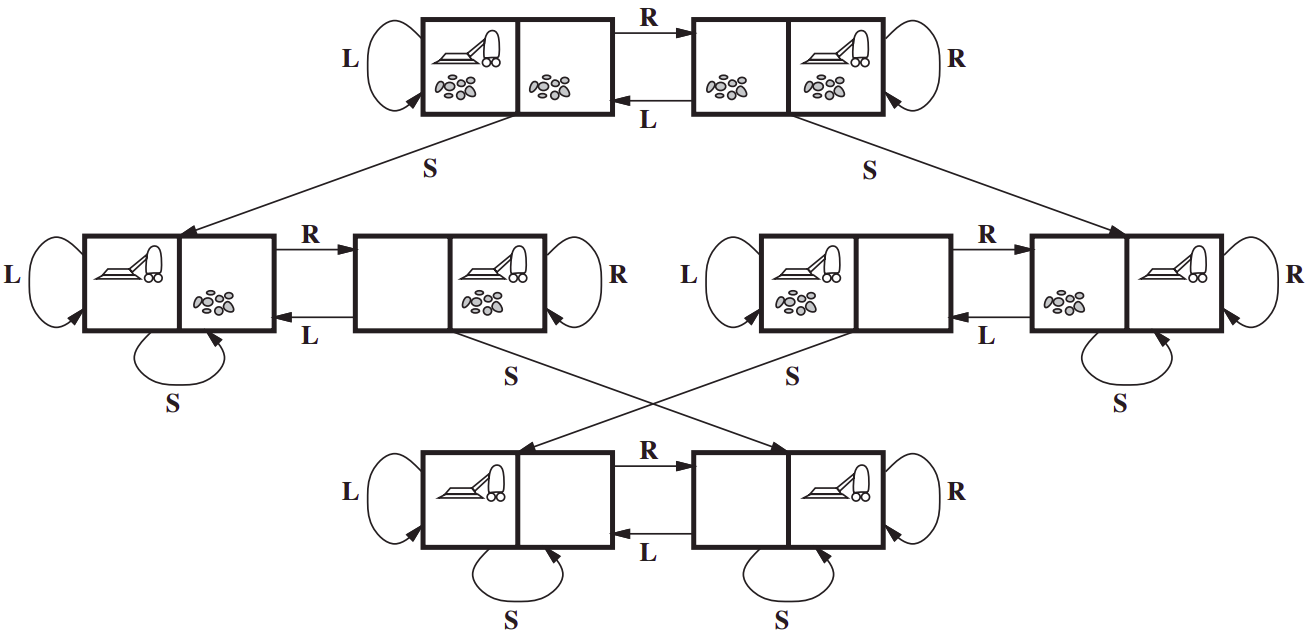
\includegraphics[
        width=\linewidth,
        % height=7cm,
        keepaspectratio
    ]{images/artificial-intelligence/examples/vacuum-state-space.png}
    \caption{The state space for the vacuum world. Links denote actions: L = Left, R = Right, S= Suck. \cite{ai/book/Artificial-Intelligence-A-Modern-Approach/Russell-Norvig}}
\end{figure}



\vspace{0.5cm}

\begin{enumerate}[itemsep=0.2cm]
    \item it’s a made-up world

    \item This particular world has just two locations: squares A and B. 
    
    \item The vacuum agent perceives which square it is in and whether there is dirt in the square. 
    
    \item It can choose to \textbf{move left}, \textbf{move right}, \textbf{suck up the dirt}, or \textbf{do nothing}.

    \item One very simple agent function is the following: if the current square is dirty, then suck; otherwise, move to the other square.

    
\end{enumerate}



\subsection{As a table driven agent}

\begin{customArrayStretch}{1.3}
\begin{longtable}{|l|l|}

\hline
\textbf{Percept sequence} & \textbf{Action} \\ \hline
\endhead

\hline
\textbf{Percept sequence} & \textbf{Action} \\ \hline
\endfirsthead

\hline\endfoot
\hline\endlastfoot


$[A, \ Clean]$ & $Right$ \\ 
$[A, \ Dirty]$ & $Suck$ \\ 
$[B, \ Clean]$ & $Left$ \\ 
$[B, \ Dirty]$ & $Suck$ \\ 

\vdots & \vdots \\

$[A, \ Clean],\ [A, \ Clean]$ & $Right$ \\ 
$[A, \ Clean],\ [A, \ Dirty]$ & $Suck$ \\ 

\vdots & \vdots \\

$[A, \ Clean],\ [A, \ Clean],\ [A, \ Clean]$ & $Right$ \\ 
$[A, \ Clean],\ [A, \ Clean],\ [A, \ Dirty]$ & $Suck$ \\ 

\vdots & \vdots \\

\end{longtable}
\end{customArrayStretch}





\subsection{As a simple reflex agent}

\begin{algorithm}[H]
    \caption{The agent program for a simple reflex agent in the two-state vacuum environment.  \cite{ai/book/Artificial-Intelligence-A-Modern-Approach/Russell-Norvig}}

    \SetKwFunction{FUNCTION}{\textsc{Reflex-Vacuum-Agent}}
    \SetKwProg{Fn}{function}{ returns \normalfont{an action}}{end}
    \Fn{\FUNCTION{[location, status]}}{
        \textbf{if} $status \ = \ Dirty$ \textbf{then return} $Suck$ \\

        \textbf{else if} $location \ = \ A$ \textbf{then return} $Right$ \\

        \textbf{else if} $location \ = \ B$ \textbf{then return} $Left$ \\
    }
\end{algorithm}







\subsection{As a problem solving agent}

\begin{enumerate}[itemsep=0.2cm]
    \item \textbf{States}: The state is determined by both the agent location and the dirt locations. The agent is in one of two locations, each of which might or might not contain dirt. Thus, there are $2 \times 2^2\ =\ 8$ possible world states. A larger environment with $n$ locations has $n \cdot 2^n$ states.

    \item \textbf{Initial state}: Any state can be designated as the initial state.

    \item \textbf{Actions}: In this simple environment, each state has just three actions: Left, Right, and Suck. Larger environments might also include Up and Down.

    \item \textbf{Transition model}: The actions have their expected effects, except that moving Left in the leftmost square, moving Right in the rightmost square, and Sucking in a clean square have no effect.

    \item \textbf{Goal test}: This checks whether all the squares are clean.

    \item \textbf{Path cost}: Each step costs $1$, so the path cost is the number of steps in the path.
\end{enumerate}

\vspace{0.5cm}

{\centering \textbf{Defining Problem \& State} \par}

\begin{lstlisting}[language=Python]
vacuumActions = ["L", "R", "S"] # L: Left, R: Right, S: Suck
vacuumSquareState = ["D", "C"] # D: Dirty, C: Clean

class VacuumState(State):
    def __init__(self, squareA, squareB, currLoc):
        self.squares = {}
        self.squares["A"] = squareA
        self.squares["B"] = squareB
        self.currLoc = currLoc

    def __str__(self):
        return (
            "<VacuumState " +
            f"squares={self.squares} "+
            f"currLoc={self.currLoc}>"
        )

    def __repr__(self) -> str:
        return str(self)

    def __eq__(self, __o: object) -> bool:
        return str(self) == str(__o)

    def copy(self):
        return VacuumState(
            self.squares["A"],
            self.squares["B"],
            self.currLoc,
        )

class VacuumProblem(Problem):
    def __init__(self, initial_state: VacuumState):
        self.initial_state = initial_state

    def step_cost(self, state: VacuumState, action: str, new_state: VacuumState):
        return (int(state.squares[state.currLoc] == "D" and action == "S")
            + int(state.currLoc == "A" and action == "R")
            + int(state.currLoc == "B" and action == "L"))

    def result(self, state: VacuumState, action: str):
        state = state.copy()

        state.currLoc = {
            "L": "A",
            "R": "B",
        }.get(action, state.currLoc)
        state.squares[state.currLoc] = {
            "S": "C"
        }.get(action, state.squares[state.currLoc])
        return state

    def actions(self, state: VacuumState):
        actions = []

        if state.squares[state.currLoc] == "D":
            actions.append("S")

        if state.currLoc == "A":
            actions.append("R")

        if state.currLoc == "B":
            actions.append("L")

        return actions

    def goal_test(self, state: VacuumState):
        return all([v == "C" for v in state.squares.values()])

init_state = VacuumState("D", "D", "A")
\end{lstlisting}



{\centering \textbf{Solution using breadth\_first\_search} \par}

\begin{lstlisting}[language=Python]
problem = VacuumProblem(init_state)
path = breadth_first_search(problem)
print(path)

node = Node(init_state, None, None, 0)
print(node)
for a in path:
    new_node = child_node(problem, node, a)
    print(a, new_node.state, new_node.path_cost, new_node)
    node = new_node
\end{lstlisting}



{\centering \textbf{Solution using uniform\_cost\_search} \par}

\begin{lstlisting}[language=Python]
problem = VacuumProblem(init_state)
path = uniform_cost_search(problem)
print(path)

node = Node(init_state, None, None, 0)
print(node)
for a in path:
    new_node = child_node(problem, node, a)
    print(a, new_node.state, new_node.path_cost, new_node)
    node = new_node
\end{lstlisting}



{\centering \textbf{Solution using depth\_first\_search} \par}

\begin{lstlisting}[language=Python]
problem = VacuumProblem(init_state)
path = depth_first_search(problem)
print(path)

node = Node(init_state, None, None, 0)
print(node)
for a in path:
    new_node = child_node(problem, node, a)
    print(a, new_node.state, new_node.path_cost, new_node)
    node = new_node
\end{lstlisting}



{\centering \textbf{Solution using backtracking\_search} \par}

\begin{lstlisting}[language=Python]
problem = VacuumProblem(init_state)
path = backtracking_search(problem)
print(path)

node = Node(init_state, None, None, 0)
print(node)
for a in path:
    new_node = child_node(problem, node, a)
    print(a, new_node.state, new_node.path_cost, new_node)
    node = new_node
\end{lstlisting}



{\centering \textbf{Solution using depth\_limited\_search} \par}

\begin{lstlisting}[language=Python]
problem = VacuumProblem(init_state)
path = depth_limited_search(problem, 5)
print(path)

node = Node(init_state, None, None, 0)
print(node)
for a in path:
    new_node = child_node(problem, node, a)
    print(a, new_node.state, new_node.path_cost, new_node)
    node = new_node

print("\n\n")

problem = VacuumProblem(init_state)
path = depth_limited_search(problem, 2)
print(path)

if isinstance(path, list):
    node = Node(init_state, None, None, 0)
    print(node)
    for a in path:
        new_node = child_node(problem, node, a)
        print(a, new_node.state, new_node.path_cost, new_node)
        node = new_node
\end{lstlisting}



{\centering \textbf{Solution using iterative\_deepening\_search} \par}

\begin{lstlisting}[language=Python]
problem = VacuumProblem(init_state)
path = iterative_deepening_search(problem)
print(path)

node = Node(init_state, None, None, 0)
print(node)
for a in path:
    new_node = child_node(problem, node, a)
    print(a, new_node.state, new_node.path_cost, new_node)
    node = new_node
\end{lstlisting}



{\centering \textbf{Solution using iterative\_lengthening\_search} \par}

\begin{lstlisting}[language=Python]
problem = VacuumProblem(init_state)
path = iterative_lengthening_search(problem)
print(path)

node = Node(init_state, None, None, 0)
print(node)
for a in path:
    new_node = child_node(problem, node, a)
    print(a, new_node.state, new_node.path_cost, new_node)
    node = new_node
\end{lstlisting}




\clearpage
\subsection{Automated Taxi Driver \cite{ai/book/Artificial-Intelligence-A-Modern-Approach/Russell-Norvig}}

\begin{enumerate}[itemsep=0.2cm]
    \item \textbf{Performance Measure}: Safe, fast, legal, comfortable trip, maximize profits
    \hfill \cite{ai/book/Artificial-Intelligence-A-Modern-Approach/Russell-Norvig}

    \item \textbf{Environment}: Roads, other traffic, pedestrians, customers
    \hfill \cite{ai/book/Artificial-Intelligence-A-Modern-Approach/Russell-Norvig}

    \item \textbf{Actuators}: Steering, accelerator, brake, signal, horn, display
    \hfill \cite{ai/book/Artificial-Intelligence-A-Modern-Approach/Russell-Norvig}

    \item \textbf{Sensors}: Cameras, sonar, speedometer, GPS, odometer, accelerometer, engine sensors, keyboard
    \hfill \cite{ai/book/Artificial-Intelligence-A-Modern-Approach/Russell-Norvig}

    \item an automated taxi cannot see what other drivers are thinking.
    \hfill \cite{ai/book/Artificial-Intelligence-A-Modern-Approach/Russell-Norvig}

    \item partially cooperative multiagent environment: avoiding collisions maximizes the performance measure of all agents
    \hfill \cite{ai/book/Artificial-Intelligence-A-Modern-Approach/Russell-Norvig}

    \item \textbf{Task Environment}: partially observable, multiagent, stochastic, sequential, dynamic, continuous, and unknown
    \hfill \cite{ai/book/Artificial-Intelligence-A-Modern-Approach/Russell-Norvig}
    
\end{enumerate}



\subsubsection{As a table driven reflex agent}

\begin{enumerate}[itemsep=0.2cm]
    \item the visual input from a single camera comes in at the rate of roughly $27$ megabytes per second ($30$ frames per second, $640 \times 480$ pixels with $24$-bits of color information). 
    \hfill \cite{ai/book/Artificial-Intelligence-A-Modern-Approach/Russell-Norvig}
    
    \item This gives a lookup table with over $10^{250,000,000,000}$ entries for \textbf{an hour}’s driving.
    \hfill \cite{ai/book/Artificial-Intelligence-A-Modern-Approach/Russell-Norvig}

    \item \textbf{Not possible} to construct the table
    \hfill \cite{ai/book/Artificial-Intelligence-A-Modern-Approach/Russell-Norvig}
\end{enumerate}



\subsubsection{As model-based reflex agents}

\begin{enumerate}[itemsep=0.2cm]
    \item the taxi may be driving back home, and it may have a rule telling it to fill up with gas on the way home unless it has at least half a tank. 
    \hfill \cite{ai/book/Artificial-Intelligence-A-Modern-Approach/Russell-Norvig}
    
    \item Although “driving back home” may seem to an aspect of the world state, the fact of the taxi’s destination is actually an aspect of the agent’s internal state. 
    \hfill \cite{ai/book/Artificial-Intelligence-A-Modern-Approach/Russell-Norvig}
    
    \item If you find this puzzling, consider that the taxi could be in exactly the same place at the same time, but intending to reach a different destination.
    \hfill \cite{ai/book/Artificial-Intelligence-A-Modern-Approach/Russell-Norvig}
    
\end{enumerate}


\subsubsection{As utility-based agents}

\begin{enumerate}[itemsep=0.2cm]
    \item \textbf{utility measures}: quicker, safer, more reliable, or cheaper 
    \hfill \cite{ai/book/Artificial-Intelligence-A-Modern-Approach/Russell-Norvig}
\end{enumerate}


\subsubsection{As Learning Agent}

\begin{enumerate}[itemsep=0.2cm]
    \item The performance element consists of whatever collection of knowledge and procedures the taxi has for selecting its driving actions.
    \hfill \cite{ai/book/Artificial-Intelligence-A-Modern-Approach/Russell-Norvig}

    \item  after the taxi makes a quick left turn across three lanes of traffic, the critic observes the shocking language used by other drivers.
    \hfill \cite{ai/book/Artificial-Intelligence-A-Modern-Approach/Russell-Norvig}

    \item From this experience, the learning element is able to formulate a rule saying this was a bad action, and the performance element is modified by installation of the new rule. 
    \hfill \cite{ai/book/Artificial-Intelligence-A-Modern-Approach/Russell-Norvig}

    
\end{enumerate}











\clearpage
\section{Road trip in Romania \cite{ai/book/Artificial-Intelligence-A-Modern-Approach/Russell-Norvig}}


\begin{figure}[H]
    \centering
    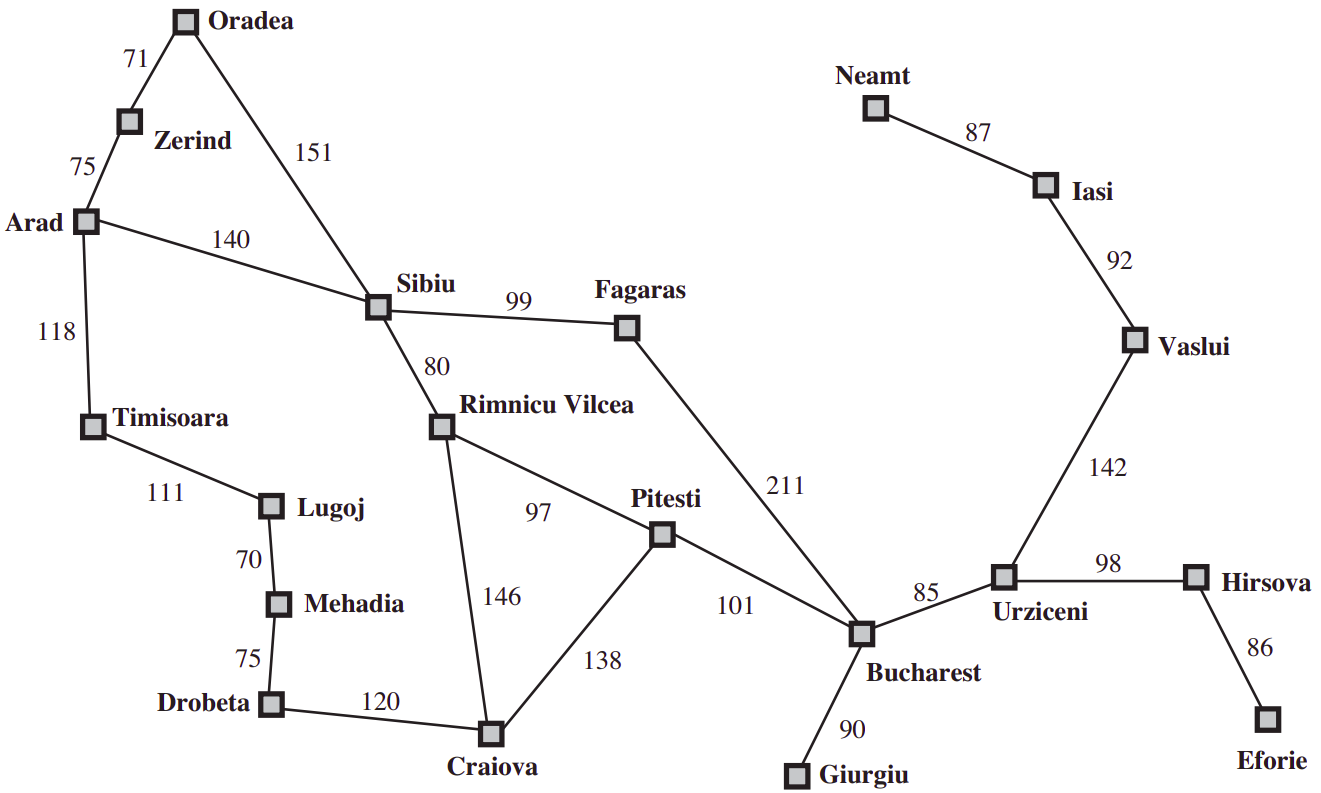
\includegraphics[
        width=\linewidth,
        height=8cm,
        keepaspectratio,
    ]{images/artificial-intelligence/examples/romania-map.png}
    \caption{A simplified road map of part of Romania. \cite{ai/book/Artificial-Intelligence-A-Modern-Approach/Russell-Norvig}}
\end{figure}


\begin{figure}[H]
    \centering
    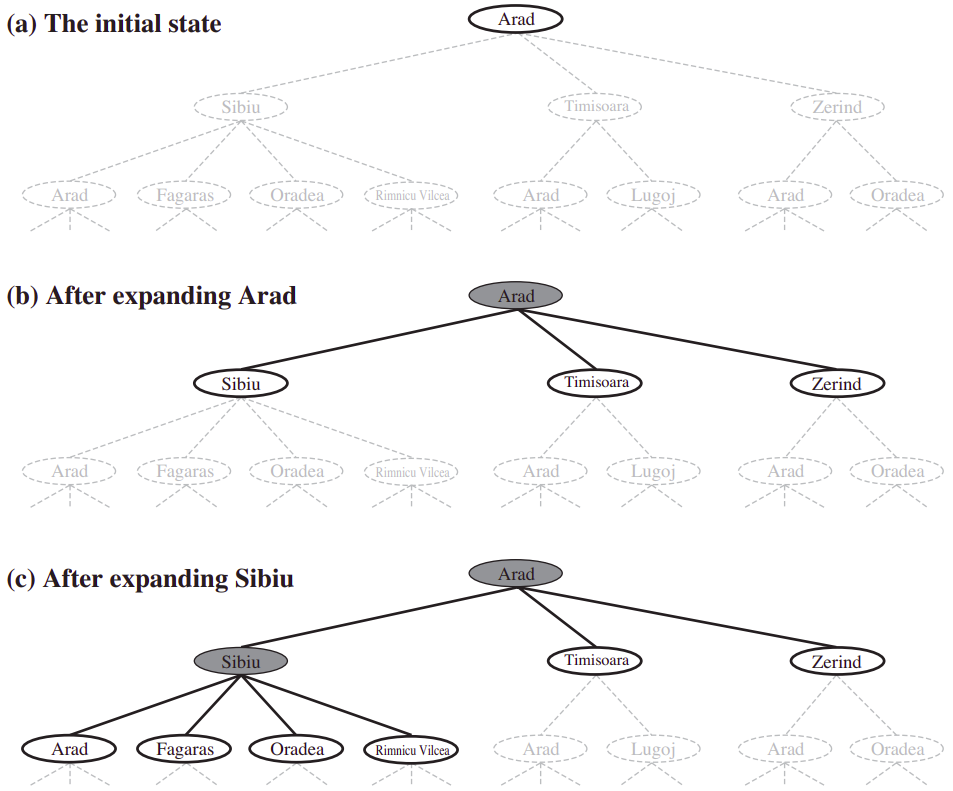
\includegraphics[
        width=\linewidth,
        height=10cm,
        keepaspectratio,
    ]{images/artificial-intelligence/examples/romania-search-tree.png}
    \caption{Partial search trees for finding a route from Arad to Bucharest. Nodes that have been expanded are shaded; nodes that have been generated but not yet expanded are outlined in bold; nodes that have not yet been generated are shown in faint dashed lines. \cite{ai/book/Artificial-Intelligence-A-Modern-Approach/Russell-Norvig}}
\end{figure}



\begin{enumerate}
    \item we use the straight-line distance (SLD) heuristic
    \hfill \cite{ai/book/Artificial-Intelligence-A-Modern-Approach/Russell-Norvig}
\end{enumerate}


\vspace{0.5cm}

{\centering \textbf{Defining Problem \& State} \par}

\begin{lstlisting}[language=Python]
# src: {tgt: path_cost}
romania_map_graph = {
    "Arad": {"Timisoara": 118, "Sibiu": 140, "Zerind": 75},
    "Bucharest": {"Pitesti": 101, "Fagaras": 211, "Giurgiu": 90, "Urziceni": 85},
    "Craiova": {"Drobeta": 120, "Rimnicu Vilcea": 146, "Pitesti": 138},
    "Drobeta": {"Mehadia": 75, "Craiova": 120},
    "Eforie": {"Hirsova": 86},
    "Fagaras": {"Sibiu": 99, "Bucharest": 211},
    "Giurgiu": {"Bucharest": 90},
    "Hirsova": {"Urziceni": 98, "Eforie": 86},
    "Iasi": {"Vaslui": 92, "Neamt": 87},
    "Lugoj": {"Mehadia": 70, "Timisoara": 111},
    "Mehadia": {"Lugoj": 70, "Drobeta": 75},
    "Neamt": {"Iasi": 87},
    "Oradea": {"Zerind": 71, "Sibiu": 151},
    "Pitesti": {"Rimnicu Vilcea": 97, "Craiova": 138, "Bucharest": 101},
    "Rimnicu Vilcea": {"Sibiu": 80, "Pitesti": 97, "Craiova": 146},
    "Sibiu": {"Fagaras": 99, "Rimnicu Vilcea": 80, "Arad": 140, "Oradea": 151},
    "Timisoara": {"Arad": 118, "Lugoj": 111},
    "Urziceni": {"Bucharest": 85, "Vaslui": 142, "Hirsova": 98},
    "Vaslui": {"Urziceni": 142, "Iasi": 92},
    "Zerind": {"Arad": 75, "Oradea": 71},
}

heuristic_Bucharest = {
    "Arad": 366,
    "Bucharest": 0,
    "Craiova": 160,
    "Drobeta": 242,
    "Eforie": 161,
    "Fagaras": 176,
    "Giurgiu": 77,
    "Hirsova": 151,
    "Iasi": 226,
    "Lugoj": 244,
    "Mehadia": 241,
    "Neamt": 234,
    "Oradea": 380,
    "Pitesti": 100,
    "Rimnicu Vilcea": 193,
    "Sibiu": 253,
    "Timisoara": 329,
    "Urziceni": 80,
    "Vaslui": 199,
    "Zerind": 374,
}


class RomaniaState(State):
    def __init__(self, city: str) -> None:
        self.city = city

    def copy(self):
        return RomaniaState(self.city)
    
    def __str__(self):
        return f"<RomaniaState city={self.city}>"

    def __repr__(self):
        return str(self)
    
    def __eq__(self, __o):
        return self.city == __o.city

class RomaniaProblem(Problem):
    def __init__(self, initial_state: RomaniaState):
        super().__init__(initial_state)
    
    def goal_test(self, state: RomaniaState):
        return state.city == "Bucharest"
    
    def step_cost(self, state: RomaniaState, action: str, new_state: RomaniaState):
        return romania_map_graph[state.city][new_state.city]
    
    def heuristic(self, state: RomaniaState):
        return heuristic_Bucharest[state.city]
    
    def actions(self, state: RomaniaState):
        return sorted(romania_map_graph[state.city].keys())
    
    def result(self, state: RomaniaState, action: str):
        return RomaniaState(action)


initial_state = RomaniaState("Arad")
problem = RomaniaProblem(initial_state=initial_state)
\end{lstlisting}



{\centering \textbf{Solution using breadth\_first\_search} \par}

\begin{lstlisting}[language=Python]
path = breadth_first_search(problem)
print(path)

node = Node(initial_state, None, None, 0)
for e in path:
    new_node = child_node(problem, node, e)
    print(
        node.state.city.ljust(20), 
        new_node.state.city.ljust(20), 
        str(new_node.path_cost - node.path_cost).rjust(5), 
        str(new_node.path_cost).rjust(5)
    )
    node = new_node
\end{lstlisting}


{\centering \textbf{Solution using uniform\_cost\_search} \par}

\begin{lstlisting}[language=Python]
path = uniform_cost_search(problem)
print(path)

node = Node(initial_state, None, None, 0)
for e in path:
    new_node = child_node(problem, node, e)
    print(
        node.state.city.ljust(20), 
        new_node.state.city.ljust(20), 
        str(new_node.path_cost - node.path_cost).rjust(5), 
        str(new_node.path_cost).rjust(5)
    )
    node = new_node
\end{lstlisting}



{\centering \textbf{Solution using depth\_first\_search} \par}

\begin{lstlisting}[language=Python]
path = depth_first_search(problem)
print(path)

node = Node(initial_state, None, None, 0)
for e in path:
    new_node = child_node(problem, node, e)
    print(
        node.state.city.ljust(20), 
        new_node.state.city.ljust(20), 
        str(new_node.path_cost - node.path_cost).rjust(5), 
        str(new_node.path_cost).rjust(5)
    )
    node = new_node
\end{lstlisting}


{\centering \textbf{Solution using backtracking\_search} \par}

\begin{lstlisting}[language=Python]
path = backtracking_search(problem)
print(path)

node = Node(initial_state, None, None, 0)
for e in path:
    new_node = child_node(problem, node, e)
    print(
        node.state.city.ljust(20), 
        new_node.state.city.ljust(20), 
        str(new_node.path_cost - node.path_cost).rjust(5), 
        str(new_node.path_cost).rjust(5)
    )
    node = new_node
\end{lstlisting}



{\centering \textbf{Solution using depth\_limited\_search} \par}

\begin{lstlisting}[language=Python]
path = depth_limited_search(problem, 4)
print(path)

node = Node(initial_state, None, None, 0)
for e in path:
    new_node = child_node(problem, node, e)
    print(
        node.state.city.ljust(20), 
        new_node.state.city.ljust(20), 
        str(new_node.path_cost - node.path_cost).rjust(5), 
        str(new_node.path_cost).rjust(5)
    )
    node = new_node

print("\n")

path = depth_limited_search(problem, 2)
print(path)

if isinstance(path, list):
    node = Node(initial_state, None, None, 0)
    for e in path:
        new_node = child_node(problem, node, e)
        print(
            node.state.city.ljust(20), 
            new_node.state.city.ljust(20), 
            str(new_node.path_cost - node.path_cost).rjust(5), 
            str(new_node.path_cost).rjust(5)
        )
        node = new_node
\end{lstlisting}


{\centering \textbf{Solution using iterative\_deepening\_search} \par}

\begin{lstlisting}[language=Python]
path = iterative_deepening_search(problem)
print(path)

node = Node(initial_state, None, None, 0)
for e in path:
    new_node = child_node(problem, node, e)
    print(
        node.state.city.ljust(20), 
        new_node.state.city.ljust(20), 
        str(new_node.path_cost - node.path_cost).rjust(5), 
        str(new_node.path_cost).rjust(5)
    )
    node = new_node
\end{lstlisting}


{\centering \textbf{Solution using iterative\_lengthening\_search} \par}

\begin{lstlisting}[language=Python]
path = iterative_lengthening_search(problem)
print(path)

node = Node(initial_state, None, None, 0)
for e in path:
    new_node = child_node(problem, node, e)
    print(
        node.state.city.ljust(20), 
        new_node.state.city.ljust(20), 
        str(new_node.path_cost - node.path_cost).rjust(5), 
        str(new_node.path_cost).rjust(5)
    )
    node = new_node
\end{lstlisting}


{\centering \textbf{Solution using A* search} \par}

\begin{figure}[H]
    \centering
    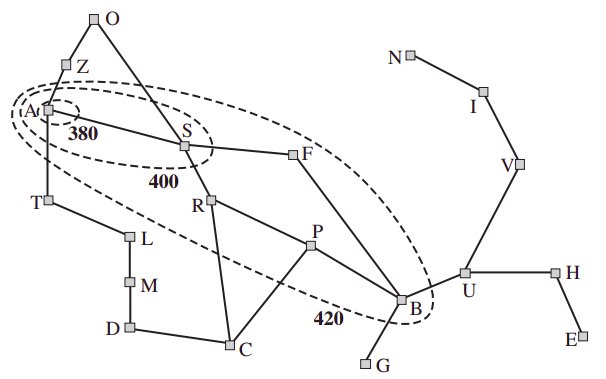
\includegraphics[
        width=\linewidth,
        height=5cm,
        keepaspectratio,
    ]{images/artificial-intelligence/examples/romania-a-star-contours.png}
    \caption{Nodes inside a given contour have f-costs less than or equal to the contour value. \cite{ai/book/Artificial-Intelligence-A-Modern-Approach/Russell-Norvig}}
\end{figure}



















\clearpage
\section{8-Puzzle \cite{ai/book/Artificial-Intelligence-A-Modern-Approach/Russell-Norvig}}

\begin{table}[H]
\begin{minipage}[t]{0.45\linewidth}
\begin{figure}[H]
    \centering
    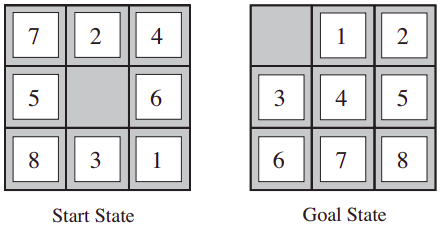
\includegraphics[
        width=\linewidth,
        height=4cm,
        keepaspectratio,
    ]{images/artificial-intelligence/examples/8-puzzle-instance-26steps.png}
    \caption{A typical instance of the 8-puzzle. The solution is 26 steps long. 
    \cite{ai/book/Artificial-Intelligence-A-Modern-Approach/Russell-Norvig}}
    \label{fig:images/artificial-intelligence/examples/8-puzzle-instance-26steps.png}
\end{figure}
\end{minipage}
\hfill
\vrule
\hfill
\begin{minipage}[t]{0.45\linewidth}
\begin{figure}[H]
    \centering
    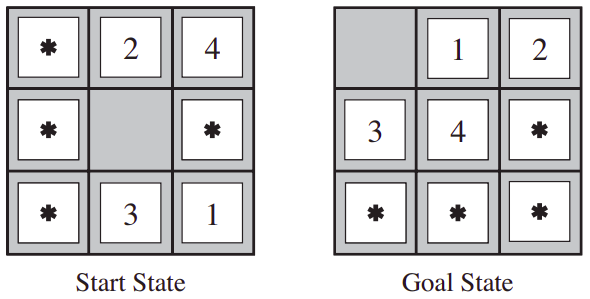
\includegraphics[
        width=\linewidth,
        height=4cm,
        keepaspectratio,
    ]{images/artificial-intelligence/examples/8-puzzle-instance-subprob-1234.png}
    \caption{A subproblem of the 8-puzzle instance. 
    The task is to get tiles 1, 2, 3, and 4 into their correct positions, without worrying about what happens to the other tiles.
    \cite{ai/book/Artificial-Intelligence-A-Modern-Approach/Russell-Norvig}}
\end{figure}
\end{minipage}
\end{table}

\begin{enumerate}[itemsep=0.2cm]
    \item the objective of the puzzle is to slide the tiles horizontally or vertically into the empty space until the configuration matches the goal configuration
    \hfill \cite{ai/book/Artificial-Intelligence-A-Modern-Approach/Russell-Norvig}

    \item The average solution cost for a randomly generated 8-puzzle instance is about $22$ steps.
    The branching factor is about $3$. 
    (When the empty tile is in the middle, four moves are possible; when it is in a corner, two; and when it is along an edge, three.) 
    This means that an exhaustive tree search to depth $22$ would look at about $3^{22} \approx 3.1 \times 10^{10}$ states.
    A \textit{graph search} would cut this down by a factor of about $170,000$ because only $9!/2$ = $181, 440$ distinct states are reachable.
    \hfill \cite{ai/book/Artificial-Intelligence-A-Modern-Approach/Russell-Norvig}

    \item if the 8-puzzle actions are described as:
    \begin{enumerate}[itemsep=0.2cm]
        \item A tile can move from square A to square B \textbf{if} A is horizontally or vertically \textit{adjacent} to B \textbf{and} B is \textit{blank}
        \hfill \cite{ai/book/Artificial-Intelligence-A-Modern-Approach/Russell-Norvig}

        \item we can generate three relaxed problems by removing one or both of the conditions:
        \begin{enumerate}
            \item A tile can move from square A to square B if A is adjacent to B.
            \hfill \cite{ai/book/Artificial-Intelligence-A-Modern-Approach/Russell-Norvig}
            
            \item A tile can move from square A to square B if B is blank.
            \hfill \cite{ai/book/Artificial-Intelligence-A-Modern-Approach/Russell-Norvig}
            
            \item A tile can move from square A to square B.
            \hfill \cite{ai/book/Artificial-Intelligence-A-Modern-Approach/Russell-Norvig}
        \end{enumerate}
    \end{enumerate}
\end{enumerate}


\subsection{Comparing heuristic functions}

two commonly used candidates:
\begin{enumerate}[itemsep=0.2cm]
    \item $h_1$: the number of misplaced tiles. 
    It is an \textbf{admissible} heuristic because it is clear that any tile that is out of place must be moved at least once.
    \hfill \cite{ai/book/Artificial-Intelligence-A-Modern-Approach/Russell-Norvig}
    \\
    All of the eight tiles are out of position, so the start state would have $h_1 = 8$.
    \hfill \cite{ai/book/Artificial-Intelligence-A-Modern-Approach/Russell-Norvig}

    \item $h_2$ = the sum of the distances of the tiles from their goal positions. 
    (city block distance or Manhattan distance)
    h2 is \textbf{admissible} because all any move can do is move one tile one step closer to the goal.
    \hfill \cite{ai/book/Artificial-Intelligence-A-Modern-Approach/Russell-Norvig}
    \\
    $h_2 = 3 + 1 + 2 + 2 + 2 + 3 + 3 + 2 = 18$
    \hfill \cite{ai/book/Artificial-Intelligence-A-Modern-Approach/Russell-Norvig}
\end{enumerate}


\subsubsection{A$^\ast$ \cite{ai/book/Artificial-Intelligence-A-Modern-Approach/Russell-Norvig}}

\begin{enumerate}[itemsep=0.2cm]
    \item $N +1=1+ b^\ast + (b^\ast)^2 + \cdots + (b^\ast)^d$
    \hfill \cite{ai/book/Artificial-Intelligence-A-Modern-Approach/Russell-Norvig}

    \item if A$^\ast$ finds a solution at depth $5$ using $52$ nodes, then the effective branching factor is $1.92$
    \hfill \cite{ai/book/Artificial-Intelligence-A-Modern-Approach/Russell-Norvig}
\end{enumerate}



\subsubsection{Comparison \cite{ai/book/Artificial-Intelligence-A-Modern-Approach/Russell-Norvig}}

\begin{customArrayStretch}{1.3}
\begin{table}[h!]
\centering
\begin{tabular}{
|
>{\RaggedLeft\arraybackslash}p{1cm}||
>{\RaggedLeft\arraybackslash}p{1.7cm}|
>{\RaggedLeft\arraybackslash}p{1.7cm}|
>{\RaggedLeft\arraybackslash}p{1.7cm}||
>{\RaggedLeft\arraybackslash}p{1.7cm}|
>{\RaggedLeft\arraybackslash}p{1.7cm}|
>{\RaggedLeft\arraybackslash}p{1.7cm}|
}


\hline


\multirow{2}{*}{$d$} & 
\multicolumn{3}{p{5.1cm}||}{\centering \textbf{Search Cost (nodes generated)}} &
\multicolumn{3}{p{5.1cm}|}{\centering \textbf{Effective Branching Factor}} \\ 

\cline{2-7}

& 
IDS & A$^\ast$($h_1$) & A$^\ast$($h_2$) & 
IDS & A$^\ast$($h_1$) & A$^\ast$($h_2$) \\ 

\hline \hline


$2$  & $10$      & $6$     & $6$     & $2.45$ & $1.79$ & $1.79$ \\ \hline
$4$  & $112$     & $13$    & $12$    & $2.87$ & $1.48$ & $1.45$ \\ \hline
$6$  & $680$     & $20$    & $18$    & $2.73$ & $1.34$ & $1.30$ \\ \hline
$8$  & $6384$    & $39$    & $25$    & $2.80$ & $1.33$ & $1.24$ \\ \hline
$10$ & $47127$   & $93$    & $39$    & $2.79$ & $1.38$ & $1.22$ \\ \hline
$12$ & $3644035$ & $227$   & $73$    & $2.78$ & $1.42$ & $1.24$ \\ \hline
$14$ & $-$       & $539$   & $113$   & $-$    & $1.44$ & $1.23$ \\ \hline
$16$ & $-$       & $1301$  & $211$   & $-$    & $1.45$ & $1.25$ \\ \hline
$18$ & $-$       & $3056$  & $363$   & $-$    & $1.46$ & $1.26$ \\ \hline
$20$ & $-$       & $7276$  & $676$   & $-$    & $1.47$ & $1.27$ \\ \hline
$22$ & $-$       & $18094$ & $1219$  & $-$    & $1.48$ & $1.28$ \\ \hline
$24$ & $-$       & $39135$ & $1641$  & $-$    & $1.48$ & $1.26$ \\ \hline


\end{tabular}
\caption{
Comparison of the search costs and effective branching factors for the \textsc{Iterative-Deepening-Search} and A$^\ast$ algorithms with $h_1$, $h_2$. 
\\
Data are averaged over $100$ instances of the $8$-puzzle for each of various solution lengths $d$.
\cite{ai/book/Artificial-Intelligence-A-Modern-Approach/Russell-Norvig}
}
\end{table}
\end{customArrayStretch}


\begin{enumerate}[itemsep=0.2cm]
    \item $h_2$ is always better than $h_1$.
    for any node $n$, $h_2(n) \geq h_1(n)$.
    \hfill \cite{ai/book/Artificial-Intelligence-A-Modern-Approach/Russell-Norvig}

    \item $h_1$ and $h_2$ are \textbf{estimates} of the remaining path length for the $8$-puzzle, but they are also \textbf{perfectly accurate} path lengths for \textbf{simplified versions} of the puzzle.
    \hfill \cite{ai/book/Artificial-Intelligence-A-Modern-Approach/Russell-Norvig}

    
\end{enumerate}




\subsubsection{Generating admissible heuristics from subproblems: Pattern databases}

\begin{enumerate}[itemsep=0.2cm]
    \item[] \textbf{Relaxed Sub-problem method}
    
    \item The choice of 1-2-3-4 is fairly arbitrary; we could also construct databases for 5-6-7-8, for 2-4-6-8, and so on.
    \hfill \cite{ai/book/Artificial-Intelligence-A-Modern-Approach/Russell-Norvig}

    \item the heuristics obtained from the 1-2-3-4 database and the 5-6-7-8 \textbf{cannot} be added
     because the solutions of the 1-2-3-4 subproblem and the 5-6-7-8 subproblem for a given state will almost certainly share some moves—it is unlikely that 1-2-3-4 can be moved into place without touching 5-6-7-8, and vice versa. 
    \hfill \cite{ai/book/Artificial-Intelligence-A-Modern-Approach/Russell-Norvig}

    \item[] \textbf{Experience method}

    \item “Experience” here means solving lots of $8$-puzzles. 
    Each optimal solution to an 8-puzzle problem provides examples from which $h(n)$ can be learned. 
    Each example consists of a state from the solution path and the actual cost of the solution from that point.
    \hfill \cite{ai/book/Artificial-Intelligence-A-Modern-Approach/Russell-Norvig}

    \item From these examples, a learning algorithm can be used to construct a function $h(n)$ that can (with luck) predict solution costs for other states that arise during search. 
    Techniques for doing this use neural nets, decision trees, and other methods or reinforcement learning.
    \hfill \cite{ai/book/Artificial-Intelligence-A-Modern-Approach/Russell-Norvig}
\end{enumerate}


























\partition{Machine Learning (ML)}
\chapter{ \emojistar Machine Learning Paradigms \cite{common/online/chatgpt}}

\begin{enumerate}
    \item Supervised Learning
    \begin{enumerate}
      \item Fully Supervised Learning
      \item Weakly Supervised Learning
      \begin{enumerate}
        \item Incomplete Supervision (e.g., partial labels)
        \item Inexact Supervision (e.g., coarse labels)
        \item Inaccurate Supervision (e.g., noisy labels)
      \end{enumerate}
    \end{enumerate}

    \item Unsupervised Learning
    \begin{enumerate}
      \item Clustering
      \item Dimensionality Reduction
      \item Density Estimation
      \item Representation Learning
    \end{enumerate}

    \item Semi-Supervised Learning
    \begin{enumerate}
      \item Transductive (train/test on same data pool)
      \item Inductive (learn general function from few labels)
    \end{enumerate}

    \item Self-Supervised Learning
    \begin{enumerate}
      \item Contrastive Learning
      \item Predictive Tasks (e.g., next token)
      \item Masked Modeling
      \item Pretext Tasks (general)
    \end{enumerate}

    \item Reinforcement Learning
    \begin{enumerate}
      \item Model-Free
      \item Model-Based \\
      \textit{(Supervision from reward signals)}
    \end{enumerate}

    \item Active Learning
    \begin{enumerate}
      \item Pool-based Sampling
      \item Stream-based Sampling
      \item Query Synthesis
    \end{enumerate}

    \item Online Learning
    \begin{enumerate}
      \item Full Information
      \item Bandit Feedback (partial feedback)
    \end{enumerate}

    \item Few-shot / One-shot / Zero-shot Learning
    \begin{enumerate}
      \item Meta-Learning
      \item Prompt-based / Embedding-based methods
    \end{enumerate}

    \item Multi-Task Learning
    \begin{enumerate}
      \item Hard Parameter Sharing
      \item Soft Parameter Sharing
    \end{enumerate}

    \item Multi-Instance Learning \\
    \textit{(Labels associated with bags of instances)}

    \item Continual / Lifelong Learning
    \begin{enumerate}
      \item Task-Incremental
      \item Domain-Incremental
      \item Class-Incremental
    \end{enumerate}

    \item Transfer Learning
    \begin{enumerate}
      \item Inductive
      \item Transductive
      \item Unsupervised Transfer
    \end{enumerate}

    \item Curriculum Learning
    \begin{enumerate}
      \item Data is presented in increasing difficulty
    \end{enumerate}
\end{enumerate}




\chapter{Machine Learning: Introduction}

\begin{enumerate}
    \item The field of machine learning is concerned with the question of how to construct computer programs that automatically improve with experience.
    \hfill \cite{ml/book/Machine-Learning/Tom-M-Mitchell}

    \item A computer program is said to \textbf{learn} from experience $E$ with respect to some class of tasks $T$ and performance measure $P$, if its performance at tasks in $T$, as measured by $P$, improves with experience $E$.
    \hfill \cite{ml/book/Machine-Learning/Tom-M-Mitchell}
    \\
    \textbf{Example}: A checkers learning problem
    \begin{enumerate}
        \item Task $T$: playing checkers
        \hfill \cite{ml/book/Machine-Learning/Tom-M-Mitchell}
        
        \item Performance measure $P$: percent of games won against opponents
        \hfill \cite{ml/book/Machine-Learning/Tom-M-Mitchell}
        
        \item Training experience $E$: playing practice games against itself 
        \hfill \cite{ml/book/Machine-Learning/Tom-M-Mitchell}
    \end{enumerate}
    
    \item \textbf{learning}: class of programs that improve through experience, not other ways like Database updates, etc
    \hfill \cite{ml/book/Machine-Learning/Tom-M-Mitchell}

    \item 
\end{enumerate}



\section{Designing A Learning System}

\subsection{Choosing the Training Experience \cite{ml/book/Machine-Learning/Tom-M-Mitchell}}

\begin{enumerate}
    \item The type of training experience available can have a \textbf{significant impact} on success or failure of the learner.
    \hfill \cite{ml/book/Machine-Learning/Tom-M-Mitchell}

    \item One key attribute is whether the training experience provides direct or indirect feedback regarding the choices made by the performance system.
    \hfill \cite{ml/book/Machine-Learning/Tom-M-Mitchell}
    \begin{enumerate}
        \item For example, in learning to play checkers, the system might learn from \textbf{direct} training examples consisting of individual checkers board states and the correct move for each.
        \hfill \cite{ml/book/Machine-Learning/Tom-M-Mitchell}

        \item it might have available only \textbf{indirect} information consisting of the move sequences and final outcomes of various games played. In this later case, information about the correctness of specific moves early in the game must be inferred indirectly from the fact that the game was eventually won or lost.
        \hfill \cite{ml/book/Machine-Learning/Tom-M-Mitchell}
    \end{enumerate}

    \item learning from direct training feedback is typically easier than learning from indirect feedback.
    \hfill \cite{ml/book/Machine-Learning/Tom-M-Mitchell}

    \item \textbf{credit assignment}: determining the degree to which each move in the sequence deserves credit or blame for the final outcome. Credit assignment can be a particularly difficult problem because the game can be lost even when early moves are optimal, if these are followed later by poor moves.
    \hfill \cite{ml/book/Machine-Learning/Tom-M-Mitchell}

    \item A second important attribute of the training experience is the \textit{degree to which the learner controls the sequence of training examples}. 
    \begin{enumerate}
        \item For example, the learner might \textbf{rely on the teacher} to select informative board states and to provide the correct move for each. 
        \hfill \cite{ml/book/Machine-Learning/Tom-M-Mitchell}

        \item Alternatively, the learner might \textbf{itself} propose board states that it finds particularly confusing and ask the teacher for the correct move.
        \hfill \cite{ml/book/Machine-Learning/Tom-M-Mitchell}

        \item Or the learner may have complete control over \textbf{both} the board states and (indirect) training classifications, as it does when it learns by playing against itself with no teacher present.
        \hfill \cite{ml/book/Machine-Learning/Tom-M-Mitchell}
        \\
        learner may choose between experimenting with novel board states that it has not yet considered, or honing its skill by playing minor variations of lines of play it currently finds most promising.
        \hfill \cite{ml/book/Machine-Learning/Tom-M-Mitchell}
    \end{enumerate}

    \item A third important attribute of the training experience is how well it represents the distribution of examples over which the final system performance $P$ must be measured.
    \hfill \cite{ml/book/Machine-Learning/Tom-M-Mitchell}
    \begin{enumerate}
        \item learning is most reliable when the training examples follow a distribution similar to that of future test examples.
        \hfill \cite{ml/book/Machine-Learning/Tom-M-Mitchell}

        \item 
        \hfill \cite{ml/book/Machine-Learning/Tom-M-Mitchell}
    \end{enumerate}
\end{enumerate}




\subsection{Choosing the Target Function ( $V$ ) }

\begin{enumerate}
    \item determine exactly what type of knowledge will be learned and how this will be used by the performance program.
    \hfill \cite{ml/book/Machine-Learning/Tom-M-Mitchell}

    \item Let us begin with a checkers-playing program that can generate the \textbf{legal moves} from any board state. The program needs only to learn how to choose the \textbf{best move} from among these legal moves.
    \hfill \cite{ml/book/Machine-Learning/Tom-M-Mitchell}

    \item function $ChooseMove$ chooses the best move for any given board state
    \hfill \cite{ml/book/Machine-Learning/Tom-M-Mitchell}

    \item it is useful to reduce the problem of improving performance $P$ at task $T$ to the problem of learning some particular target function.
    \hfill \cite{ml/book/Machine-Learning/Tom-M-Mitchell}

    \item $ChooseMove : B \to M$ indicates that this function accepts as input any board from the set of legal board states $B$ and produces as output some move from the set of legal moves $M$.
    \hfill \cite{ml/book/Machine-Learning/Tom-M-Mitchell}

    \item let \textbf{evaluation function}: $V$
    \hfill \cite{ml/book/Machine-Learning/Tom-M-Mitchell}

    \item notation $V : B \to \mbbR$ denote that $V$ maps any legal board state from the set $B$ to some real value (we use $\mbbR$ to denote the set of real numbers). We intend for this target function $V$ to assign higher scores to better board states. If the system can successfully learn such a target function $V$, then it can easily use it to select the best move from any current board position.
    \hfill \cite{ml/book/Machine-Learning/Tom-M-Mitchell}

    \item This can be accomplished by generating the successor board state produced by every legal move, then using $V$ to choose the best successor state and therefore the best legal move. 
    \hfill \cite{ml/book/Machine-Learning/Tom-M-Mitchell}

    \item \textbf{operational description of $V$}: description that can be used by the checkers-playing program to evaluate states and select moves within realistic time bounds
    \hfill \cite{ml/book/Machine-Learning/Tom-M-Mitchell}
    \\
    \textbf{nonoperational definition}: definition is not efficiently computable
    \hfill \cite{ml/book/Machine-Learning/Tom-M-Mitchell}

    \item It may be very difficult in general to learn such an operational form of $V$ perfectly. In fact, we often expect learning algorithms to acquire only some approximation to the target function, and for this reason the process of learning the target function is often called \textbf{function approximation} ( $\hat{V}$ ).
    \hfill \cite{ml/book/Machine-Learning/Tom-M-Mitchell}

    \item In general, this choice of representation ( $\hat{V}$ ) involves a crucial tradeoff.
    \\
    On one hand, we wish to pick a very expressive representation to allow representing as close an approximation as possible to the ideal target function $V$.
    \\
    On the other hand, the more expressive the representation, the more training data the program will require in order to choose among the alternative hypotheses it can represent.
    \hfill \cite{ml/book/Machine-Learning/Tom-M-Mitchell}



    \item[] \textbf{example}: Let:
    \\
    $x_1$: the number of black pieces on the board 
    \\
    $x_2$: the number of red pieces on the board 
    \\
    $x_3$: the number of black kings on the board 
    \\
    $x_4$: the number of red kings on the board 
    \\
    $x_5$: the number of black pieces threatened by red (i.e., which can be captured on red's next turn) 
    \\
    $x_6$: the number of red pieces threatened by black 
    \vspace{0.3cm} \noindent
    \\
    Then: 
    \\
    Partial design of a checkers learning program: 
    \\ \\
    .\hfill \textbf{(specification of the learning task)} \hfill.
    \\ \\
    Task $T$: playing checkers 
    \\
    Performance measure $P$: percent of games won in the world tournament 
    \\
    Training experience $E$: games played against itself 
    \\ \\
    .\hfill \textbf{(design choices for the implementation of the learning program)} \hfill.
    \\ \\
    Target function: $V: Board \to \mbbR$ 
    \\
    Target function representation: $\hat{V}(b) = w_0 + w_1x_1 + w_2x_2 + w_3x_3 + w_4x_4 + w_5x_5 + w_6x_6$ 
    \\
    where $w_0$ through $w_6$ are numerical coefficients, or weights, to be chosen by the learning algorithm. Learned values for the weights $w_1$ through $w_6$ will determine the relative importance of the various board features in determining the value of the board, whereas the weight $w_0$ will provide an additive constant to the board value. 
    
    \item each training example: $\dAngleBrac{b, V_{train}(b)}$
        \hfill (board state $b$; training value $V_{train}(b)$ for $b$)

    \item the fact that the game was eventually won or lost does not necessarily indicate that every board state along the game path was necessarily good or bad.
    \hfill \cite{ml/book/Machine-Learning/Tom-M-Mitchell}
    \\
    For example, even if the program loses the game, it may still be the case that board states occurring early in the game should be rated very highly and that the cause of the loss was a subsequent poor move. 
    \hfill \cite{ml/book/Machine-Learning/Tom-M-Mitchell}

    \item Despite the ambiguity inherent in estimating training values for intermediate board states, one simple approach has been found to be surprisingly successful.
    This approach is to assign the training value of $V_{train}(b)$ for any intermediate board state $b$ to be $\hat{V}(Successor(b))$, where $\hat{V}$ is the learner's current approximation to $V$ and where $Successor(b)$ denotes the next board state following $b$ for which it is again the program's turn to move.
    \hfill \cite{ml/book/Machine-Learning/Tom-M-Mitchell}

    \item 
    \textbf{Rule for estimating training values}: $V_{train}(b) \gets \hat{V}(Successor(b))$
    \hfill \cite{ml/book/Machine-Learning/Tom-M-Mitchell}
    
    \item 
    $\hat{V}(Successor(b))$ = training value of $V_{train}(b)$ for any intermediate board state $b$
    \\
    .\hspace{1cm} $\hat{V}$ is the learner's current approximation to $V$
    \\
    .\hspace{1cm} $Successor(b)$ denotes the next board state following $b$
    \vspace{0.3cm} \noindent
    
\end{enumerate}





































\partition{Recurrent Neural Networks (RNNs)}
\chapter{Recurrent Neural Networks (RNN)}




















\chapter{Bi-directional RNN}














\chapter{Long Short-Term Memory (LSTM)}













\partition{Advanced ML Techniques}
\chapter{Encoder-Decoder Architecture}

AKA Sequence-to-Sequence (seq2seq)

\begin{enumerate}
    \item An \textbf{encoder} neural network reads and encodes an input sequence into a \textbf{fixed-length vector}. 
    \hfill \cite{adv-ml-tech/paper/arxiv.org/1409.0473}
    
    \item A \textbf{decoder} then outputs from the encoded vector.
    \hfill \cite{adv-ml-tech/paper/arxiv.org/1409.0473}
\end{enumerate}


\section{Disadvantages}
\begin{enumerate}
    \item A potential issue with this encoder–decoder approach is that a neural network needs to be able to compress all the necessary information of a source sentence into a fixed-length vector.
    \hfill \cite{adv-ml-tech/paper/arxiv.org/1409.0473}

    \item This may make it difficult for the neural network to cope with long sequences, especially those that are longer than the sequences in the training corpus. 
    \hfill \cite{adv-ml-tech/paper/arxiv.org/1409.0473}

    \item  performance of a basic encoder–decoder deteriorates rapidly as the length of an input sequence increases.
    \hfill \cite{adv-ml-tech/paper/arxiv.org/1409.0473}
\end{enumerate}













\chapter{Attention Mechanism (2014)}

\begin{center}
    \textbf{Source}: \cite{adv-ml-tech/paper/arxiv.org/1409.0473},
    \textbf{General Context Extracted Using}: \cite{common/online/chatgpt}
\end{center}


\begin{enumerate}
    \item allows the model to dynamically and softly focus on different parts of the input when generating each part of the output, without needing to explicitly isolate those parts in advance.
    \hfill \cite{adv-ml-tech/paper/arxiv.org/1409.0473, common/online/chatgpt}

    \item This approach leads to improved results and produces attention patterns that align with human intuition about which input elements are most relevant at each step.
    \hfill \cite{adv-ml-tech/paper/arxiv.org/1409.0473, common/online/chatgpt}

    \item an extension to the sequence model that learns to align relevant parts of the input while generating the output.
    \hfill \cite{adv-ml-tech/paper/arxiv.org/1409.0473, common/online/chatgpt}

    \item At each step of output generation, the model softly identifies positions in the input sequence that contain the most relevant information.
    It then uses this focused context, along with all previously generated outputs, to predict the next output element.
    \hfill \cite{adv-ml-tech/paper/arxiv.org/1409.0473, common/online/chatgpt}

    \item it avoids compressing the entire input into a single fixed-length vector. Instead, it encodes the input sequence into a sequence of vectors and adaptively selects a subset of these vectors during output generation.
    This removes the burden of forcing all input information—regardless of length—into one compact representation, enabling the model to handle longer inputs more effectively.
    \hfill \cite{adv-ml-tech/paper/arxiv.org/1409.0473, common/online/chatgpt}


\end{enumerate}


\section{Architecture}


\begin{enumerate}
    \item input: $x = (x_1, \cdots, x_{T_x})$
    \hfill \cite{adv-ml-tech/paper/arxiv.org/1409.0473}
\end{enumerate}

\subsection{Encoder: a Bi-directional RNN}

\begin{enumerate}
    \item hidden states/ \textbf{annotations}: $(h_1, \cdots, h_{T_x})$
    \hfill \cite{adv-ml-tech/paper/arxiv.org/1409.0473}
    \begin{enumerate}
        \item  Each annotation $h_i$ contains information about the whole input sequence with a strong focus on the parts surrounding the $i$-th word of the input sequence.
        \hfill \cite{adv-ml-tech/paper/arxiv.org/1409.0473}
    \end{enumerate}


    \item Forward RNN ($\overset{\rightarrow}{f}$) reads the input sequence as it is ordered (from $x_1$ to $x_{T_x}$ ) and calculates a sequence of forward hidden states ( $\overset{\rightarrow}{h}_1, \cdots , \overset{\rightarrow}{h}_{T_x}$ ).
    \hfill \cite{adv-ml-tech/paper/arxiv.org/1409.0473}

    \item backward RNN ($\overset{\leftarrow}{f}$) reads the sequence in the reverse order (from $x_{T_x}$ to $x_1$), resulting in a sequence of backward hidden states ( $\overset{\leftarrow}{h}_1, \cdots , \overset{\leftarrow}{h}_{T_x}$ ).
    \hfill \cite{adv-ml-tech/paper/arxiv.org/1409.0473}

    \item  annotation for each word $x_j$ by concatenating the forward hidden state $\overset{\rightarrow}{h} _j$ and the backward one $\overset{\leftarrow}{h} _j$
    \hfill \cite{adv-ml-tech/paper/arxiv.org/1409.0473}
    \\
    .\hfill
    $
        h_j = \dSquareBrac{
            \overset{\rightarrow}{h} _j^\top ; \
            \overset{\leftarrow}{h} _j^\top
        }
    $
    \hfill \cite{adv-ml-tech/paper/arxiv.org/1409.0473}
    \\
    In this way, the annotation $h_j$ contains the summaries of both the preceding words and the following words.
    \hfill \cite{adv-ml-tech/paper/arxiv.org/1409.0473}

    \item Due to the tendency of RNNs to better represent recent inputs, the annotation $h_j$ will be focused on the words around $x_j$.
    \hfill \cite{adv-ml-tech/paper/arxiv.org/1409.0473}
\end{enumerate}

\subsection{Decoder}

\begin{enumerate}
    \item emulates searching through source sequence during decoding
    \hfill \cite{adv-ml-tech/paper/arxiv.org/1409.0473}

    \item decoder hidden state: $s_i = f(s_{i-1}, y_{i-1}, c_i)$
    \hfill \cite{adv-ml-tech/paper/arxiv.org/1409.0473}

    \item conditional probability: $P(y_i | y_1, \cdots , y_{i-1}, x) = g(y_{i-1}, s_i, c_i)$
    \hfill \cite{adv-ml-tech/paper/arxiv.org/1409.0473}


    \item context vector: $c_i$ depends on annotations:
    $
        c_i
        = \dsum_{j=1}^{T_x} \alpha_{ij} h_j
    $
    \hfill \cite{adv-ml-tech/paper/arxiv.org/1409.0473}
    \begin{enumerate}
        \item aka expected annotation
        \hfill \cite{adv-ml-tech/paper/arxiv.org/1409.0473}

        \item $\alpha_{ij}$:  probability that the target word $y_i$ is aligned to, or translated from, a source word $x_j$
        \hfill \cite{adv-ml-tech/paper/arxiv.org/1409.0473}

        \item $i$-th context vector $c_i$ is the expected annotation over all the annotations with probabilities $\alpha_{ij}$
        \hfill \cite{adv-ml-tech/paper/arxiv.org/1409.0473}
    \end{enumerate}



    \item weight $\alpha_{ij}$ of each annotation $h_j$:
    $
        \alpha_{ij}
        = \dfrac{exp(e_{ij})}{\tsum_{k=1}^T exp(e_{ik})}
    $
    \hfill \cite{adv-ml-tech/paper/arxiv.org/1409.0473}

    \item alignment model/ energy: $e_{ij} = a(s_{i-1}, h_j)$\\
    scores how well the inputs around position $j$ and the output at position $i$ match.
    \hfill \cite{adv-ml-tech/paper/arxiv.org/1409.0473}

    \item  We parametrize the alignment model a as a feedforward neural network which is jointly trained with all the other components of the proposed system.
    \hfill \cite{adv-ml-tech/paper/arxiv.org/1409.0473}

    \item the alignment is not considered to be a latent variable.
    Instead, the alignment model directly computes a soft alignment, which allows the gradient of the cost function to be backpropagated through.
    This gradient can be used to train the alignment model as well as the whole translation model jointly.
    \hfill \cite{adv-ml-tech/paper/arxiv.org/1409.0473}

    \item The probability $\alpha_{ij}$, or its associated energy $e_{ij}$, reflects the importance of the annotation $h_j$ with respect to the previous hidden state $s_{i-1}$ in deciding the next state $s_i$ and generating $y_i$.
    \hfill \cite{adv-ml-tech/paper/arxiv.org/1409.0473}

    \item This implements a mechanism of attention in the decoder.
    The decoder decides parts of the source sentence to pay attention to.
    By letting the decoder have an attention mechanism, we relieve the encoder from the burden of having to encode all information in the source sentence into a fixed-length vector.
    \hfill \cite{adv-ml-tech/paper/arxiv.org/1409.0473}


\end{enumerate}






























\partition{Applications}
\chapter{Statistical Machine Translation}













\chapter{Neural Machine Translation (NMT)}

\section{Intro}

\begin{enumerate}
    \item Translate sentences from one language to another using Neural Networks (NNs)
\end{enumerate}


\subsection{Probabilistic Perspective}

\begin{enumerate}
    \item translation is equivalent to finding a target sentence $y$ that maximizes the conditional probability of $y$ given a source sentence $x$, i.e., $\arg\max_y p(y | x)$.
    \hfill \cite{adv-ml-tech/paper/arxiv.org/1409.0473}

    \item  we fit a parameterized model to maximize the conditional probability of sentence pairs using a parallel training corpus.
    \hfill \cite{adv-ml-tech/paper/arxiv.org/1409.0473}

    \item Once the conditional distribution is learned by a translation model, given a source sentence a corresponding translation can be generated by searching for the sentence that maximizes the conditional probability.
    \hfill \cite{adv-ml-tech/paper/arxiv.org/1409.0473}
\end{enumerate}


















\section{Encoder-decoder Models}

\begin{enumerate}
    \item An encoder neural network reads and encodes a source sentence into a fixed-length vector.
    \hfill \cite{adv-ml-tech/paper/arxiv.org/1409.0473}
    
    \item A decoder then outputs a translation from the encoded vector. 
    \hfill \cite{adv-ml-tech/paper/arxiv.org/1409.0473}

    \item The whole encoder–decoder system, which consists of the encoder and the decoder for a language pair, is jointly trained to maximize the probability of a correct translation given a source sentence.
    \hfill \cite{adv-ml-tech/paper/arxiv.org/1409.0473}
\end{enumerate}





\subsection{RNN Encoder-Decoder}
\begin{enumerate}
    \item encode a variable-length source sentence into a fixed-length vector and to decode the vector into a variable-length target sentence.
    \hfill \cite{adv-ml-tech/paper/arxiv.org/1409.0473}

    \item Encoder:
    \begin{enumerate}
        \item reads the input sentence: sequence of vectors $x = (x_1, \cdots, x_{T_x})$
        \hfill \cite{adv-ml-tech/paper/arxiv.org/1409.0473}

        \item $h_t = f(x_t, h_{t-1}) \in \mathbb{R}^n$ : hidden state at time $t$
        \hfill \cite{adv-ml-tech/paper/arxiv.org/1409.0473}

        \item $c = q(\dCurlyBrac{h_1, \cdots, h_{T_x}})$ :  vector generated from the sequence of the hidden states
        \hfill \cite{adv-ml-tech/paper/arxiv.org/1409.0473}

        \item $f$ and $q$ are some nonlinear functions
        \hfill \cite{adv-ml-tech/paper/arxiv.org/1409.0473}
    \end{enumerate}

    \item Decoder:
    \begin{enumerate}
        \item trained to predict the next word $y_{t^\prime}$ given the context vector $c$ and all the previously predicted words $\dCurlyBrac{y_1, \cdots , y_{t^\prime-1}}$. 
        \hfill \cite{adv-ml-tech/paper/arxiv.org/1409.0473}

        \item In other words, the decoder defines a probability over the translation $y$ by decomposing the joint probability into the ordered conditionals:\\
        $
            p(y)
            = \dprod_{t=1}^T p(y_t | \dCurlyBrac{y_1, \cdots, y_{t-1}}, c)
        $
        \hfill \cite{adv-ml-tech/paper/arxiv.org/1409.0473}
        \\
        where $y = (y_1, \cdots, y_{T_y})$
        \hfill \cite{adv-ml-tech/paper/arxiv.org/1409.0473}
        \\
        For RNN: 
        $
            p(y_t | \dCurlyBrac{y_1, \cdots, y_{t-1}}, c)
            = g(y_{t-1}, s_t, c)
        $
        \hfill \cite{adv-ml-tech/paper/arxiv.org/1409.0473}
        
        \item $g$ is a nonlinear, potentially multi-layered, function that outputs the probability of $y_t$
        \hfill \cite{adv-ml-tech/paper/arxiv.org/1409.0473}

        \item $s_t$ hidden state of decoder RNN
        \hfill \cite{adv-ml-tech/paper/arxiv.org/1409.0473}
    \end{enumerate}
\end{enumerate}







\subsubsection{LSTM Encoder-Decoder}
\begin{enumerate}
    \item achieves close to the state-of-the-art performance of the conventional phrase-based machine translation system
    \hfill \cite{adv-ml-tech/paper/arxiv.org/1409.0473}

    \item LSTM is used as $f$ and $c = q(\dCurlyBrac{h_1, \cdots, h_{T_x}}) = h_{T_x}$ in encoder part of RNN Encoder-Decoder
    \hfill \cite{adv-ml-tech/paper/arxiv.org/1409.0473}
\end{enumerate}










\subsection{Attention-Based Encoder-Decoder Models}

\begin{enumerate}
    \item learns to align and translate jointly
    \hfill \cite{adv-ml-tech/paper/arxiv.org/1409.0473}

    \item Each time the model generates a word in a translation, it (soft-)searches for a set of positions in a source sentence where the most relevant information is concentrated. 
    The model then predicts a target word based on the context vectors associated with these source positions and all the previous generated target words.
    \hfill \cite{adv-ml-tech/paper/arxiv.org/1409.0473}

    \item it does not attempt to encode a whole input sentence into a single fixed-length vector.
    Instead, it encodes the input sentence into a sequence of vectors and chooses a subset of these vectors adaptively while decoding the translation. 
    This frees a neural translation model from having to squash all the information of a source sentence, regardless of its length, into a fixed-length vector.
    \hfill \cite{adv-ml-tech/paper/arxiv.org/1409.0473}
\end{enumerate}















\partition{Appendix}
\chapter{Datasets}\label{Datasets}



\begin{customArrayStretch}{1.3}
\begin{longtable}{
    |
    >{\RaggedRight\arraybackslash}p{5cm}| % Dataset Name
    >{\hfill}p{2.5cm}| % Size
    >{\hfill}p{3cm}| % Records/ Items
    >{\hfill}p{2cm}| % Remarks
}

\hline
    \textsc{Dataset Name} & 
    \textsc{Size} (\verb|du -sh|) & 
    \textsc{Records/ Items} & 
    \textsc{Source(s)} \\
\hline
\endfirsthead

\hline
    \textsc{Dataset Name} & 
    \textsc{Size} (\verb|du -sh|) & 
    \textsc{Records/ Items} & 
    \textsc{Source(s)} \\
\hline
\endhead

\hline \endfoot
\hline \endlastfoot

%%%%%%%%%%%%%%%%%%%%%%%%%%%%%%%%%%%%%%%%%%%%%%%%%%%%%%%%%%%%%%%%%%%%%%%%%%%%%%%%%%%%%%%%%%



\href{http://www.nth-iteration.com/wp-content/uploads/2018/08/demographics-synthetic.csv}{Demographics Synthetic} \label{Datasets/nth-iteration/demographics-synthetic} & 
$24$K &
$(500, 6)$ & 
\cite{statistics/book/Statistics-for-Data-Scientists/Maurits-Kaptein} \\ \hline

\href{http://www.nth-iteration.com/wp-content/uploads/2018/08/face-data.csv}{Face Data} \label{Datasets/nth-iteration/face-data} & 
$260$K &
$(3628, 7)$ & 
\cite{statistics/book/Statistics-for-Data-Scientists/Maurits-Kaptein} \\ \hline

\href{http://www.nth-iteration.com/wp-content/uploads/2018/08/high-school.csv}{High School} \label{Datasets/nth-iteration/high-school} & 
$2.4$M &
$(50069, 13)$ & 
\cite{statistics/book/Statistics-for-Data-Scientists/Maurits-Kaptein} \\ \hline

\href{http://www.nth-iteration.com/wp-content/uploads/2018/08/houses.csv}{Houses} \label{Datasets/nth-iteration/houses} & 
$32$K &
$(546, 13)$ & 
\cite{statistics/book/Statistics-for-Data-Scientists/Maurits-Kaptein} \\ \hline

\href{https://drive.google.com/file/d/1GYUk0i9penKnSWODDkZfMzNxK2FUxDi8/view?usp=drive_link}{Potatoes} \label{Datasets/nth-iteration/potatoes} & 
$876$K &
$(47582, 7)$ & 
\cite{statistics/book/Statistics-for-Data-Scientists/Maurits-Kaptein} \\ \hline

\href{http://www.nth-iteration.com/wp-content/uploads/2018/08/voting_demo.csv}{Voting Demo} \label{Datasets/nth-iteration/voting_demo} & 
$36$K &
$(750, 7)$ & 
\cite{statistics/book/Statistics-for-Data-Scientists/Maurits-Kaptein} \\ \hline



\href{https://drive.google.com/file/d/1DKQnolgdVxQddQAp1haafo0AqvFVT5yj/view?usp=drive_link}{Sampling Plans - Population}  &
$8.9$M &
$(50000, 25)$ &
\cite{common/online/chatgpt} \\ \hline






%%%%%%%%%%%%%%%%%%%%%%%%%%%%%%%%%%%%%%%%%%%%%%%%%%%%%%%%%%%%%%%%%%%%%%%%%%%%%%%%%%%%%%%%%%

\end{longtable}
\end{customArrayStretch}









\label{MMLastPage}
\cleardoublepage



%-------------------------
%	Additional pages
%-------------------------

\backmatter
\pagestyle{empty}
\cleardoublepage
\pagenumbering{roman}
\pagestyle{extra}


\nocite{*}

\defbibheading{bibempty}{\chapter*{References}}


\clearpage
{
    % Save original geometry and fancyhdr settings
    \newgeometry{left=1cm, right=1cm, top=1cm, bottom=2cm} % Leave bottom margin large enough for footer

    \setlength{\columnsep}{15pt}
    % \begin{multicols}{2}

    \raggedright
    \printbibliography[heading=bibempty]

    % \end{multicols}

    \restoregeometry
    \thispagestyle{fancy} % Restore footer on this page
}

\end{document}
